\documentclass[twoside]{book}

% Packages required by doxygen
\usepackage{fixltx2e}
\usepackage{calc}
\usepackage{doxygen}
\usepackage{graphicx}
\usepackage[utf8]{inputenc}
\usepackage{makeidx}
\usepackage{multicol}
\usepackage{multirow}
\PassOptionsToPackage{warn}{textcomp}
\usepackage{textcomp}
\usepackage[nointegrals]{wasysym}
\usepackage[table]{xcolor}
\usepackage{ifpdf,ifxetex}

% Font selection
\usepackage[T1]{fontenc}
\usepackage[scaled=.90]{helvet}
\usepackage{courier}
\usepackage{amssymb}
\usepackage{sectsty}
\renewcommand{\familydefault}{\sfdefault}
\allsectionsfont{%
  \fontseries{bc}\selectfont%
  \color{darkgray}%
}
\renewcommand{\DoxyLabelFont}{%
  \fontseries{bc}\selectfont%
  \color{darkgray}%
}
\newcommand{\+}{\discretionary{\mbox{\scriptsize$\hookleftarrow$}}{}{}}

% Page & text layout
\usepackage{geometry}
\geometry{%
  a4paper,%
  top=2.5cm,%
  bottom=2.5cm,%
  left=2.5cm,%
  right=2.5cm%
}
\tolerance=750
\hfuzz=15pt
\hbadness=750
\setlength{\emergencystretch}{15pt}
\setlength{\parindent}{0cm}
\setlength{\parskip}{3ex plus 2ex minus 2ex}
\makeatletter
\renewcommand{\paragraph}{%
  \@startsection{paragraph}{4}{0ex}{-1.0ex}{1.0ex}{%
    \normalfont\normalsize\bfseries\SS@parafont%
  }%
}
\renewcommand{\subparagraph}{%
  \@startsection{subparagraph}{5}{0ex}{-1.0ex}{1.0ex}{%
    \normalfont\normalsize\bfseries\SS@subparafont%
  }%
}
\makeatother

% Headers & footers
\usepackage{fancyhdr}
\pagestyle{fancyplain}
\fancyhead[LE]{\fancyplain{}{\bfseries\thepage}}
\fancyhead[CE]{\fancyplain{}{}}
\fancyhead[RE]{\fancyplain{}{\bfseries\leftmark}}
\fancyhead[LO]{\fancyplain{}{\bfseries\rightmark}}
\fancyhead[CO]{\fancyplain{}{}}
\fancyhead[RO]{\fancyplain{}{\bfseries\thepage}}
\fancyfoot[LE]{\fancyplain{}{}}
\fancyfoot[CE]{\fancyplain{}{}}
\fancyfoot[RE]{\fancyplain{}{\bfseries\scriptsize Generated by Doxygen }}
\fancyfoot[LO]{\fancyplain{}{\bfseries\scriptsize Generated by Doxygen }}
\fancyfoot[CO]{\fancyplain{}{}}
\fancyfoot[RO]{\fancyplain{}{}}
\renewcommand{\footrulewidth}{0.4pt}
\renewcommand{\chaptermark}[1]{%
  \markboth{#1}{}%
}
\renewcommand{\sectionmark}[1]{%
  \markright{\thesection\ #1}%
}

% Indices & bibliography
\usepackage{natbib}
\usepackage[titles]{tocloft}
\setcounter{tocdepth}{3}
\setcounter{secnumdepth}{5}
\makeindex

% Hyperlinks (required, but should be loaded last)
\ifpdf
  \usepackage[pdftex,pagebackref=true]{hyperref}
\else
  \ifxetex
    \usepackage[pagebackref=true]{hyperref}
  \else
    \usepackage[ps2pdf,pagebackref=true]{hyperref}
  \fi
\fi
\ifpdf
  \DeclareUnicodeCharacter{207B}{${}^{-}$}% Superscript minus
  \DeclareUnicodeCharacter{C2B2}{${}^{2}$}% Superscript two
  \DeclareUnicodeCharacter{C2B3}{${}^{3}$}% Superscript three
\else
  \catcode`\⁻=13% Superscript minus
  \def⁻{${}^{-}$}
  \catcode`\²=13% Superscript two
  \def²{${}^{2}$}
  \catcode`\³=13% Superscript three
  \def³{${}^{3}$}
\fi

\hypersetup{%
  colorlinks=true,%
  linkcolor=blue,%
  citecolor=blue,%
  unicode%
}

% Custom commands
\newcommand{\clearemptydoublepage}{%
  \newpage{\pagestyle{empty}\cleardoublepage}%
}

\usepackage{caption}
\captionsetup{labelsep=space,justification=centering,font={bf},singlelinecheck=off,skip=4pt,position=top}

\renewcommand{\numberline}[1]{#1~}
%===== C O N T E N T S =====

\begin{document}

% Titlepage & ToC
\hypersetup{pageanchor=false,
             bookmarksnumbered=true,
             pdfencoding=unicode
            }
\pagenumbering{alph}
\begin{titlepage}
\vspace*{7cm}
\begin{center}%
{\Large Mapping Museums webapp }\\
\vspace*{1cm}
{\large Generated by Doxygen 1.8.15}\\
\end{center}
\end{titlepage}
\clearemptydoublepage
\pagenumbering{roman}
\tableofcontents
\clearemptydoublepage
\pagenumbering{arabic}
\hypersetup{pageanchor=true}

%--- Begin generated contents ---
\chapter{Hierarchical Index}
\section{Class Hierarchy}
This inheritance list is sorted roughly, but not completely, alphabetically\+:\begin{DoxyCompactList}
\item \contentsline{section}{app.\+main.\+boksplots.\+bokehcategorybar.\+Bokeh\+Category\+Bar}{\pageref{classapp_1_1main_1_1boksplots_1_1bokehcategorybar_1_1BokehCategoryBar}}{}
\item \contentsline{section}{app.\+main.\+boksplots.\+bokehcategorypie.\+Bokeh\+Category\+Pie}{\pageref{classapp_1_1main_1_1boksplots_1_1bokehcategorypie_1_1BokehCategoryPie}}{}
\item \contentsline{section}{app.\+main.\+boksplots.\+bokehheatmap.\+Bokeh\+Heatmap}{\pageref{classapp_1_1main_1_1boksplots_1_1bokehheatmap_1_1BokehHeatmap}}{}
\item \contentsline{section}{app.\+main.\+boksplots.\+bokehtime.\+Bokeh\+Time}{\pageref{classapp_1_1main_1_1boksplots_1_1bokehtime_1_1BokehTime}}{}
\item \contentsline{section}{app.\+main.\+boksplots.\+bokehtimeandcategory.\+Bokeh\+Time\+And\+Category}{\pageref{classapp_1_1main_1_1boksplots_1_1bokehtimeandcategory_1_1BokehTimeAndCategory}}{}
\item \contentsline{section}{app.\+main.\+boksplots.\+bokehtree.\+Bokeh\+Tree}{\pageref{classapp_1_1main_1_1boksplots_1_1bokehtree_1_1BokehTree}}{}
\item \contentsline{section}{app.\+main.\+boks.\+Boks}{\pageref{classapp_1_1main_1_1boks_1_1Boks}}{}
\item \contentsline{section}{app.\+main.\+chloro.\+Chloro}{\pageref{classapp_1_1main_1_1chloro_1_1Chloro}}{}
\item \contentsline{section}{app.\+main.\+boks.\+Boks.\+closings\+\_\+over\+\_\+time}{\pageref{classapp_1_1main_1_1boks_1_1Boks_1_1closings__over__time}}{}
\item \contentsline{section}{app.\+main.\+Configuration.\+Configuration}{\pageref{classapp_1_1main_1_1Configuration_1_1Configuration}}{}
\item \contentsline{section}{app.\+main.\+boksplots.\+custompie.\+Custom\+Pie\+Builder}{\pageref{classapp_1_1main_1_1boksplots_1_1custompie_1_1CustomPieBuilder}}{}
\item dict\begin{DoxyCompactList}
\item \contentsline{section}{app.\+main.\+P\+Tree\+Node.\+P\+Tree\+Node}{\pageref{classapp_1_1main_1_1PTreeNode_1_1PTreeNode}}{}
\end{DoxyCompactList}
\item Exception\begin{DoxyCompactList}
\item \contentsline{section}{app.\+main.\+treelib.\+exceptions.\+Duplicated\+Node\+Id\+Error}{\pageref{classapp_1_1main_1_1treelib_1_1exceptions_1_1DuplicatedNodeIdError}}{}
\item \contentsline{section}{app.\+main.\+treelib.\+exceptions.\+Invalid\+Level\+Number}{\pageref{classapp_1_1main_1_1treelib_1_1exceptions_1_1InvalidLevelNumber}}{}
\item \contentsline{section}{app.\+main.\+treelib.\+exceptions.\+Link\+Past\+Root\+Node\+Error}{\pageref{classapp_1_1main_1_1treelib_1_1exceptions_1_1LinkPastRootNodeError}}{}
\item \contentsline{section}{app.\+main.\+treelib.\+exceptions.\+Loop\+Error}{\pageref{classapp_1_1main_1_1treelib_1_1exceptions_1_1LoopError}}{}
\item \contentsline{section}{app.\+main.\+treelib.\+exceptions.\+Multiple\+Root\+Error}{\pageref{classapp_1_1main_1_1treelib_1_1exceptions_1_1MultipleRootError}}{}
\item \contentsline{section}{app.\+main.\+treelib.\+exceptions.\+Node\+Property\+Error}{\pageref{classapp_1_1main_1_1treelib_1_1exceptions_1_1NodePropertyError}}{}
\begin{DoxyCompactList}
\item \contentsline{section}{app.\+main.\+treelib.\+exceptions.\+Node\+I\+D\+Absent\+Error}{\pageref{classapp_1_1main_1_1treelib_1_1exceptions_1_1NodeIDAbsentError}}{}
\item \contentsline{section}{app.\+main.\+treelib.\+exceptions.\+Node\+Property\+Absent\+Error}{\pageref{classapp_1_1main_1_1treelib_1_1exceptions_1_1NodePropertyAbsentError}}{}
\end{DoxyCompactList}
\end{DoxyCompactList}
\item \contentsline{section}{app.\+main.\+mapchart.\+Map\+Chart}{\pageref{classapp_1_1main_1_1mapchart_1_1MapChart}}{}
\item \contentsline{section}{app.\+main.\+nakedid.\+Naked\+Id}{\pageref{classapp_1_1main_1_1nakedid_1_1NakedId}}{}
\item object\begin{DoxyCompactList}
\item \contentsline{section}{app.\+main.\+datatypes.\+Admin\+\_\+\+Area.\+Admin\+\_\+\+Area}{\pageref{classapp_1_1main_1_1datatypes_1_1Admin__Area_1_1Admin__Area}}{}
\item \contentsline{section}{app.\+main.\+datatypes.\+Governance\+\_\+\+Change.\+Governance\+\_\+\+Change}{\pageref{classapp_1_1main_1_1datatypes_1_1Governance__Change_1_1Governance__Change}}{}
\item \contentsline{section}{app.\+main.\+datatypes.\+Visitor\+\_\+\+Numbers\+\_\+\+Data.\+Visitor\+\_\+\+Numbers\+\_\+\+Data}{\pageref{classapp_1_1main_1_1datatypes_1_1Visitor__Numbers__Data_1_1Visitor__Numbers__Data}}{}
\item \contentsline{section}{app.\+main.\+model\+\_\+to\+\_\+view.\+Model\+\_\+\+To\+\_\+\+View}{\pageref{classapp_1_1main_1_1model__to__view_1_1Model__To__View}}{}
\item \contentsline{section}{app.\+main.\+tree.\+Tree}{\pageref{classapp_1_1main_1_1tree_1_1Tree}}{}
\item \contentsline{section}{app.\+main.\+treelib.\+node.\+Node}{\pageref{classapp_1_1main_1_1treelib_1_1node_1_1Node}}{}
\item \contentsline{section}{app.\+main.\+treelib.\+tree.\+Tree}{\pageref{classapp_1_1main_1_1treelib_1_1tree_1_1Tree}}{}
\end{DoxyCompactList}
\item \contentsline{section}{app.\+main.\+boks.\+Boks.\+open\+\_\+at\+\_\+a\+\_\+given\+\_\+time}{\pageref{classapp_1_1main_1_1boks_1_1Boks_1_1open__at__a__given__time}}{}
\item \contentsline{section}{app.\+main.\+boks.\+Boks.\+open\+\_\+over\+\_\+time}{\pageref{classapp_1_1main_1_1boks_1_1Boks_1_1open__over__time}}{}
\item \contentsline{section}{app.\+main.\+boks.\+Boks.\+openings\+\_\+and\+\_\+closings\+\_\+over\+\_\+time}{\pageref{classapp_1_1main_1_1boks_1_1Boks_1_1openings__and__closings__over__time}}{}
\item \contentsline{section}{app.\+main.\+boks.\+Boks.\+openings\+\_\+over\+\_\+time}{\pageref{classapp_1_1main_1_1boks_1_1Boks_1_1openings__over__time}}{}
\item \contentsline{section}{app.\+main.\+search.\+Search}{\pageref{classapp_1_1main_1_1search_1_1Search}}{}
\item \contentsline{section}{app.\+main.\+showmuseumtypes.\+Show\+Museum\+Types}{\pageref{classapp_1_1main_1_1showmuseumtypes_1_1ShowMuseumTypes}}{}
\item \contentsline{section}{app.\+main.\+boks.\+Boks.\+test\+\_\+of\+\_\+heatmap}{\pageref{classapp_1_1main_1_1boks_1_1Boks_1_1test__of__heatmap}}{}
\item \contentsline{section}{app.\+main.\+boks.\+Boks.\+that\+\_\+opened\+\_\+up\+\_\+to\+\_\+a\+\_\+given\+\_\+time}{\pageref{classapp_1_1main_1_1boks_1_1Boks_1_1that__opened__up__to__a__given__time}}{}
\item Method\+View\begin{DoxyCompactList}
\item \contentsline{section}{app.\+main.\+admingeoservice.\+Admingeoservice}{\pageref{classapp_1_1main_1_1admingeoservice_1_1Admingeoservice}}{}
\item \contentsline{section}{app.\+main.\+datasetversionservice.\+Datasetversionservice}{\pageref{classapp_1_1main_1_1datasetversionservice_1_1Datasetversionservice}}{}
\end{DoxyCompactList}
\item View\begin{DoxyCompactList}
\item \contentsline{section}{app.\+main.\+views.\+App\+Configuration}{\pageref{classapp_1_1main_1_1views_1_1AppConfiguration}}{}
\end{DoxyCompactList}
\end{DoxyCompactList}

\chapter{Class Index}
\section{Class List}
Here are the classes, structs, unions and interfaces with brief descriptions\+:\begin{DoxyCompactList}
\item\contentsline{section}{\mbox{\hyperlink{classapp_1_1main_1_1datatypes_1_1Admin__Area_1_1Admin__Area}{app.\+main.\+datatypes.\+Admin\+\_\+\+Area.\+Admin\+\_\+\+Area}} }{\pageref{classapp_1_1main_1_1datatypes_1_1Admin__Area_1_1Admin__Area}}{}
\item\contentsline{section}{\mbox{\hyperlink{classapp_1_1main_1_1admingeoservice_1_1Admingeoservice}{app.\+main.\+admingeoservice.\+Admingeoservice}} }{\pageref{classapp_1_1main_1_1admingeoservice_1_1Admingeoservice}}{}
\item\contentsline{section}{\mbox{\hyperlink{classapp_1_1main_1_1views_1_1AppConfiguration}{app.\+main.\+views.\+App\+Configuration}} }{\pageref{classapp_1_1main_1_1views_1_1AppConfiguration}}{}
\item\contentsline{section}{\mbox{\hyperlink{classapp_1_1main_1_1boksplots_1_1bokehcategorybar_1_1BokehCategoryBar}{app.\+main.\+boksplots.\+bokehcategorybar.\+Bokeh\+Category\+Bar}} }{\pageref{classapp_1_1main_1_1boksplots_1_1bokehcategorybar_1_1BokehCategoryBar}}{}
\item\contentsline{section}{\mbox{\hyperlink{classapp_1_1main_1_1boksplots_1_1bokehcategorypie_1_1BokehCategoryPie}{app.\+main.\+boksplots.\+bokehcategorypie.\+Bokeh\+Category\+Pie}} }{\pageref{classapp_1_1main_1_1boksplots_1_1bokehcategorypie_1_1BokehCategoryPie}}{}
\item\contentsline{section}{\mbox{\hyperlink{classapp_1_1main_1_1boksplots_1_1bokehheatmap_1_1BokehHeatmap}{app.\+main.\+boksplots.\+bokehheatmap.\+Bokeh\+Heatmap}} }{\pageref{classapp_1_1main_1_1boksplots_1_1bokehheatmap_1_1BokehHeatmap}}{}
\item\contentsline{section}{\mbox{\hyperlink{classapp_1_1main_1_1boksplots_1_1bokehtime_1_1BokehTime}{app.\+main.\+boksplots.\+bokehtime.\+Bokeh\+Time}} }{\pageref{classapp_1_1main_1_1boksplots_1_1bokehtime_1_1BokehTime}}{}
\item\contentsline{section}{\mbox{\hyperlink{classapp_1_1main_1_1boksplots_1_1bokehtimeandcategory_1_1BokehTimeAndCategory}{app.\+main.\+boksplots.\+bokehtimeandcategory.\+Bokeh\+Time\+And\+Category}} }{\pageref{classapp_1_1main_1_1boksplots_1_1bokehtimeandcategory_1_1BokehTimeAndCategory}}{}
\item\contentsline{section}{\mbox{\hyperlink{classapp_1_1main_1_1boksplots_1_1bokehtree_1_1BokehTree}{app.\+main.\+boksplots.\+bokehtree.\+Bokeh\+Tree}} }{\pageref{classapp_1_1main_1_1boksplots_1_1bokehtree_1_1BokehTree}}{}
\item\contentsline{section}{\mbox{\hyperlink{classapp_1_1main_1_1boks_1_1Boks}{app.\+main.\+boks.\+Boks}} }{\pageref{classapp_1_1main_1_1boks_1_1Boks}}{}
\item\contentsline{section}{\mbox{\hyperlink{classapp_1_1main_1_1chloro_1_1Chloro}{app.\+main.\+chloro.\+Chloro}} }{\pageref{classapp_1_1main_1_1chloro_1_1Chloro}}{}
\item\contentsline{section}{\mbox{\hyperlink{classapp_1_1main_1_1boks_1_1Boks_1_1closings__over__time}{app.\+main.\+boks.\+Boks.\+closings\+\_\+over\+\_\+time}} }{\pageref{classapp_1_1main_1_1boks_1_1Boks_1_1closings__over__time}}{}
\item\contentsline{section}{\mbox{\hyperlink{classapp_1_1main_1_1Configuration_1_1Configuration}{app.\+main.\+Configuration.\+Configuration}} }{\pageref{classapp_1_1main_1_1Configuration_1_1Configuration}}{}
\item\contentsline{section}{\mbox{\hyperlink{classapp_1_1main_1_1boksplots_1_1custompie_1_1CustomPieBuilder}{app.\+main.\+boksplots.\+custompie.\+Custom\+Pie\+Builder}} }{\pageref{classapp_1_1main_1_1boksplots_1_1custompie_1_1CustomPieBuilder}}{}
\item\contentsline{section}{\mbox{\hyperlink{classapp_1_1main_1_1datasetversionservice_1_1Datasetversionservice}{app.\+main.\+datasetversionservice.\+Datasetversionservice}} }{\pageref{classapp_1_1main_1_1datasetversionservice_1_1Datasetversionservice}}{}
\item\contentsline{section}{\mbox{\hyperlink{classapp_1_1main_1_1treelib_1_1exceptions_1_1DuplicatedNodeIdError}{app.\+main.\+treelib.\+exceptions.\+Duplicated\+Node\+Id\+Error}} }{\pageref{classapp_1_1main_1_1treelib_1_1exceptions_1_1DuplicatedNodeIdError}}{}
\item\contentsline{section}{\mbox{\hyperlink{classapp_1_1main_1_1datatypes_1_1Governance__Change_1_1Governance__Change}{app.\+main.\+datatypes.\+Governance\+\_\+\+Change.\+Governance\+\_\+\+Change}} }{\pageref{classapp_1_1main_1_1datatypes_1_1Governance__Change_1_1Governance__Change}}{}
\item\contentsline{section}{\mbox{\hyperlink{classapp_1_1main_1_1treelib_1_1exceptions_1_1InvalidLevelNumber}{app.\+main.\+treelib.\+exceptions.\+Invalid\+Level\+Number}} }{\pageref{classapp_1_1main_1_1treelib_1_1exceptions_1_1InvalidLevelNumber}}{}
\item\contentsline{section}{\mbox{\hyperlink{classapp_1_1main_1_1treelib_1_1exceptions_1_1LinkPastRootNodeError}{app.\+main.\+treelib.\+exceptions.\+Link\+Past\+Root\+Node\+Error}} }{\pageref{classapp_1_1main_1_1treelib_1_1exceptions_1_1LinkPastRootNodeError}}{}
\item\contentsline{section}{\mbox{\hyperlink{classapp_1_1main_1_1treelib_1_1exceptions_1_1LoopError}{app.\+main.\+treelib.\+exceptions.\+Loop\+Error}} }{\pageref{classapp_1_1main_1_1treelib_1_1exceptions_1_1LoopError}}{}
\item\contentsline{section}{\mbox{\hyperlink{classapp_1_1main_1_1mapchart_1_1MapChart}{app.\+main.\+mapchart.\+Map\+Chart}} }{\pageref{classapp_1_1main_1_1mapchart_1_1MapChart}}{}
\item\contentsline{section}{\mbox{\hyperlink{classapp_1_1main_1_1model__to__view_1_1Model__To__View}{app.\+main.\+model\+\_\+to\+\_\+view.\+Model\+\_\+\+To\+\_\+\+View}} \\*Purpose\+:Formats a model representation to a view representation of all datatypes }{\pageref{classapp_1_1main_1_1model__to__view_1_1Model__To__View}}{}
\item\contentsline{section}{\mbox{\hyperlink{classapp_1_1main_1_1treelib_1_1exceptions_1_1MultipleRootError}{app.\+main.\+treelib.\+exceptions.\+Multiple\+Root\+Error}} }{\pageref{classapp_1_1main_1_1treelib_1_1exceptions_1_1MultipleRootError}}{}
\item\contentsline{section}{\mbox{\hyperlink{classapp_1_1main_1_1nakedid_1_1NakedId}{app.\+main.\+nakedid.\+Naked\+Id}} }{\pageref{classapp_1_1main_1_1nakedid_1_1NakedId}}{}
\item\contentsline{section}{\mbox{\hyperlink{classapp_1_1main_1_1treelib_1_1node_1_1Node}{app.\+main.\+treelib.\+node.\+Node}} }{\pageref{classapp_1_1main_1_1treelib_1_1node_1_1Node}}{}
\item\contentsline{section}{\mbox{\hyperlink{classapp_1_1main_1_1treelib_1_1exceptions_1_1NodeIDAbsentError}{app.\+main.\+treelib.\+exceptions.\+Node\+I\+D\+Absent\+Error}} }{\pageref{classapp_1_1main_1_1treelib_1_1exceptions_1_1NodeIDAbsentError}}{}
\item\contentsline{section}{\mbox{\hyperlink{classapp_1_1main_1_1treelib_1_1exceptions_1_1NodePropertyAbsentError}{app.\+main.\+treelib.\+exceptions.\+Node\+Property\+Absent\+Error}} }{\pageref{classapp_1_1main_1_1treelib_1_1exceptions_1_1NodePropertyAbsentError}}{}
\item\contentsline{section}{\mbox{\hyperlink{classapp_1_1main_1_1treelib_1_1exceptions_1_1NodePropertyError}{app.\+main.\+treelib.\+exceptions.\+Node\+Property\+Error}} }{\pageref{classapp_1_1main_1_1treelib_1_1exceptions_1_1NodePropertyError}}{}
\item\contentsline{section}{\mbox{\hyperlink{classapp_1_1main_1_1boks_1_1Boks_1_1open__at__a__given__time}{app.\+main.\+boks.\+Boks.\+open\+\_\+at\+\_\+a\+\_\+given\+\_\+time}} }{\pageref{classapp_1_1main_1_1boks_1_1Boks_1_1open__at__a__given__time}}{}
\item\contentsline{section}{\mbox{\hyperlink{classapp_1_1main_1_1boks_1_1Boks_1_1open__over__time}{app.\+main.\+boks.\+Boks.\+open\+\_\+over\+\_\+time}} }{\pageref{classapp_1_1main_1_1boks_1_1Boks_1_1open__over__time}}{}
\item\contentsline{section}{\mbox{\hyperlink{classapp_1_1main_1_1boks_1_1Boks_1_1openings__and__closings__over__time}{app.\+main.\+boks.\+Boks.\+openings\+\_\+and\+\_\+closings\+\_\+over\+\_\+time}} }{\pageref{classapp_1_1main_1_1boks_1_1Boks_1_1openings__and__closings__over__time}}{}
\item\contentsline{section}{\mbox{\hyperlink{classapp_1_1main_1_1boks_1_1Boks_1_1openings__over__time}{app.\+main.\+boks.\+Boks.\+openings\+\_\+over\+\_\+time}} }{\pageref{classapp_1_1main_1_1boks_1_1Boks_1_1openings__over__time}}{}
\item\contentsline{section}{\mbox{\hyperlink{classapp_1_1main_1_1PTreeNode_1_1PTreeNode}{app.\+main.\+P\+Tree\+Node.\+P\+Tree\+Node}} \\*Purpose\+:Removes type info from name Arguments\+: }{\pageref{classapp_1_1main_1_1PTreeNode_1_1PTreeNode}}{}
\item\contentsline{section}{\mbox{\hyperlink{classapp_1_1main_1_1search_1_1Search}{app.\+main.\+search.\+Search}} }{\pageref{classapp_1_1main_1_1search_1_1Search}}{}
\item\contentsline{section}{\mbox{\hyperlink{classapp_1_1main_1_1showmuseumtypes_1_1ShowMuseumTypes}{app.\+main.\+showmuseumtypes.\+Show\+Museum\+Types}} }{\pageref{classapp_1_1main_1_1showmuseumtypes_1_1ShowMuseumTypes}}{}
\item\contentsline{section}{\mbox{\hyperlink{classapp_1_1main_1_1boks_1_1Boks_1_1test__of__heatmap}{app.\+main.\+boks.\+Boks.\+test\+\_\+of\+\_\+heatmap}} }{\pageref{classapp_1_1main_1_1boks_1_1Boks_1_1test__of__heatmap}}{}
\item\contentsline{section}{\mbox{\hyperlink{classapp_1_1main_1_1boks_1_1Boks_1_1that__opened__up__to__a__given__time}{app.\+main.\+boks.\+Boks.\+that\+\_\+opened\+\_\+up\+\_\+to\+\_\+a\+\_\+given\+\_\+time}} }{\pageref{classapp_1_1main_1_1boks_1_1Boks_1_1that__opened__up__to__a__given__time}}{}
\item\contentsline{section}{\mbox{\hyperlink{classapp_1_1main_1_1treelib_1_1tree_1_1Tree}{app.\+main.\+treelib.\+tree.\+Tree}} }{\pageref{classapp_1_1main_1_1treelib_1_1tree_1_1Tree}}{}
\item\contentsline{section}{\mbox{\hyperlink{classapp_1_1main_1_1tree_1_1Tree}{app.\+main.\+tree.\+Tree}} }{\pageref{classapp_1_1main_1_1tree_1_1Tree}}{}
\item\contentsline{section}{\mbox{\hyperlink{classapp_1_1main_1_1datatypes_1_1Visitor__Numbers__Data_1_1Visitor__Numbers__Data}{app.\+main.\+datatypes.\+Visitor\+\_\+\+Numbers\+\_\+\+Data.\+Visitor\+\_\+\+Numbers\+\_\+\+Data}} }{\pageref{classapp_1_1main_1_1datatypes_1_1Visitor__Numbers__Data_1_1Visitor__Numbers__Data}}{}
\end{DoxyCompactList}

\chapter{File Index}
\section{File List}
Here is a list of all documented files with brief descriptions\+:\begin{DoxyCompactList}
\item\contentsline{section}{/home/nlarsson/bbk/python/webdev/museumflask/app/main/\mbox{\hyperlink{admingeoservice_8py}{admingeoservice.\+py}} \\*~\newline
 This is an A\+PI service for the search front end to provide locations from the geo graph that matches the users characters as they type }{\pageref{admingeoservice_8py}}{}
\item\contentsline{section}{/home/nlarsson/bbk/python/webdev/museumflask/app/main/\mbox{\hyperlink{apputils_8py}{apputils.\+py}} \\*This module implements \+: 1 }{\pageref{apputils_8py}}{}
\item\contentsline{section}{/home/nlarsson/bbk/python/webdev/museumflask/app/main/\mbox{\hyperlink{boks_8py}{boks.\+py}} \\*~\newline
 This class is the entry point for all plots in the visualise page }{\pageref{boks_8py}}{}
\item\contentsline{section}{/home/nlarsson/bbk/python/webdev/museumflask/app/main/\mbox{\hyperlink{chloro_8py}{chloro.\+py}} \\*This class implements the choropleths used for the various regions }{\pageref{chloro_8py}}{}
\item\contentsline{section}{/home/nlarsson/bbk/python/webdev/museumflask/app/main/\mbox{\hyperlink{Configuration_8py}{Configuration.\+py}} \\*~\newline
 Implements a configuration to be stored in the DB }{\pageref{Configuration_8py}}{}
\item\contentsline{section}{/home/nlarsson/bbk/python/webdev/museumflask/app/main/\mbox{\hyperlink{datasetversionservice_8py}{datasetversionservice.\+py}} \\*~\newline
 The api service to return the data set version }{\pageref{datasetversionservice_8py}}{}
\item\contentsline{section}{/home/nlarsson/bbk/python/webdev/museumflask/app/main/\mbox{\hyperlink{definitions_8py}{definitions.\+py}} \\*~\newline
 This module implements all strings used in the code as well as lookup dictionaries,lists and file names }{\pageref{definitions_8py}}{}
\item\contentsline{section}{/home/nlarsson/bbk/python/webdev/museumflask/app/main/\mbox{\hyperlink{errors_8py}{errors.\+py}} \\*~\newline
 F\+L\+A\+SK error handlers }{\pageref{errors_8py}}{}
\item\contentsline{section}{/home/nlarsson/bbk/python/webdev/museumflask/app/main/\mbox{\hyperlink{listman_8py}{listman.\+py}} \\*~\newline
 ~\newline
 ~\newline
 ~\newline
 ~\newline
 ~\newline
 ~\newline
 ~\newline
 ~\newline
 ~\newline
 ~\newline
 More details }{\pageref{listman_8py}}{}
\item\contentsline{section}{/home/nlarsson/bbk/python/webdev/museumflask/app/main/\mbox{\hyperlink{mapchart_8py}{mapchart.\+py}} \\*This class implements the map page view }{\pageref{mapchart_8py}}{}
\item\contentsline{section}{/home/nlarsson/bbk/python/webdev/museumflask/app/main/\mbox{\hyperlink{model__to__view_8py}{model\+\_\+to\+\_\+view.\+py}} \\*~\newline
 This class defines operations that allows to go from model representation of a variable to view representation and this is used mostly in search to format output from the database }{\pageref{model__to__view_8py}}{}
\item\contentsline{section}{/home/nlarsson/bbk/python/webdev/museumflask/app/main/\mbox{\hyperlink{models_8py}{models.\+py}} \\*~\newline
 This module initialises the O\+NS dictionaries,all configuration lists, and builds the datatype dictionary through database introspection }{\pageref{models_8py}}{}
\item\contentsline{section}{/home/nlarsson/bbk/python/webdev/museumflask/app/main/\mbox{\hyperlink{nakedid_8py}{nakedid.\+py}} \\*~\newline
 This class implements the view to show a specific museum with ID ~\newline
 It has two views; view default or view all }{\pageref{nakedid_8py}}{}
\item\contentsline{section}{/home/nlarsson/bbk/python/webdev/museumflask/app/main/\mbox{\hyperlink{PTreeNode_8py}{P\+Tree\+Node.\+py}} \\*Simple tree implementation }{\pageref{PTreeNode_8py}}{}
\item\contentsline{section}{/home/nlarsson/bbk/python/webdev/museumflask/app/main/\mbox{\hyperlink{tree_8py}{tree.\+py}} \\*Builds the menu tree for browse }{\pageref{tree_8py}}{}
\item\contentsline{section}{/home/nlarsson/bbk/python/webdev/museumflask/app/main/\mbox{\hyperlink{views_8py}{views.\+py}} \\*~\newline
 Contains the F\+L\+A\+SK views and their html implementation and routing }{\pageref{views_8py}}{}
\item\contentsline{section}{/home/nlarsson/bbk/python/webdev/museumflask/app/main/datatypes/\mbox{\hyperlink{Admin__Area_8py}{Admin\+\_\+\+Area.\+py}} \\*~\newline
 Implementation of a datatype follows this interface which has to be implemented\+: }{\pageref{Admin__Area_8py}}{}
\item\contentsline{section}{/home/nlarsson/bbk/python/webdev/museumflask/app/main/datatypes/\mbox{\hyperlink{Governance__Change_8py}{Governance\+\_\+\+Change.\+py}} \\*~\newline
 Implementation of a datatype follows this interface which has to be implemented\+: }{\pageref{Governance__Change_8py}}{}
\item\contentsline{section}{/home/nlarsson/bbk/python/webdev/museumflask/app/main/datatypes/\mbox{\hyperlink{Visitor__Numbers__Data_8py}{Visitor\+\_\+\+Numbers\+\_\+\+Data.\+py}} \\*~\newline
 Implementation of a datatype follows this interface which has to be implemented\+: }{\pageref{Visitor__Numbers__Data_8py}}{}
\end{DoxyCompactList}

\chapter{Class Documentation}
\hypertarget{classapp_1_1main_1_1datatypes_1_1Admin__Area_1_1Admin__Area}{}\section{app.\+main.\+datatypes.\+Admin\+\_\+\+Area.\+Admin\+\_\+\+Area Class Reference}
\label{classapp_1_1main_1_1datatypes_1_1Admin__Area_1_1Admin__Area}\index{app.\+main.\+datatypes.\+Admin\+\_\+\+Area.\+Admin\+\_\+\+Area@{app.\+main.\+datatypes.\+Admin\+\_\+\+Area.\+Admin\+\_\+\+Area}}
Inheritance diagram for app.\+main.\+datatypes.\+Admin\+\_\+\+Area.\+Admin\+\_\+\+Area\+:\begin{figure}[H]
\begin{center}
\leavevmode
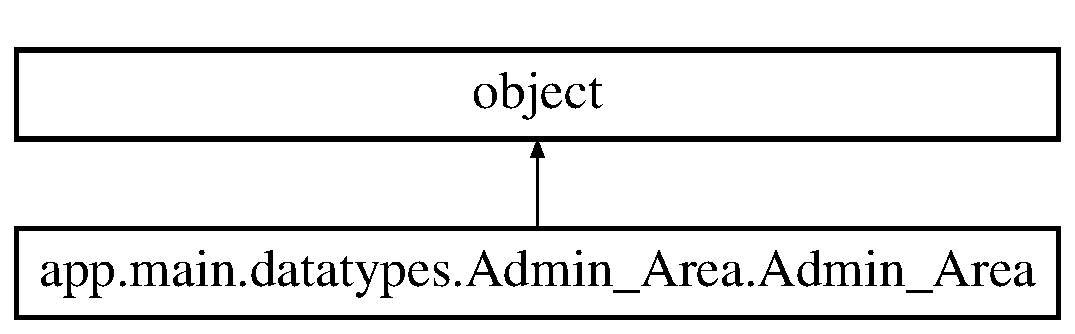
\includegraphics[height=2.000000cm]{classapp_1_1main_1_1datatypes_1_1Admin__Area_1_1Admin__Area}
\end{center}
\end{figure}
\subsection*{Public Member Functions}
\begin{DoxyCompactItemize}
\item 
\mbox{\Hypertarget{classapp_1_1main_1_1datatypes_1_1Admin__Area_1_1Admin__Area_ab1b3d88cfabc030d45e8b5ae6c710a52}\label{classapp_1_1main_1_1datatypes_1_1Admin__Area_1_1Admin__Area_ab1b3d88cfabc030d45e8b5ae6c710a52}} 
def {\bfseries \+\_\+\+\_\+init\+\_\+\+\_\+} (self)
\end{DoxyCompactItemize}


The documentation for this class was generated from the following file\+:\begin{DoxyCompactItemize}
\item 
/home/nlarsson/bbk/python/webdev/museumflask/app/main/datatypes/\mbox{\hyperlink{Admin__Area_8py}{Admin\+\_\+\+Area.\+py}}\end{DoxyCompactItemize}

\hypertarget{classapp_1_1main_1_1admingeoservice_1_1Admingeoservice}{}\section{app.\+main.\+admingeoservice.\+Admingeoservice Class Reference}
\label{classapp_1_1main_1_1admingeoservice_1_1Admingeoservice}\index{app.\+main.\+admingeoservice.\+Admingeoservice@{app.\+main.\+admingeoservice.\+Admingeoservice}}
Inheritance diagram for app.\+main.\+admingeoservice.\+Admingeoservice\+:\begin{figure}[H]
\begin{center}
\leavevmode
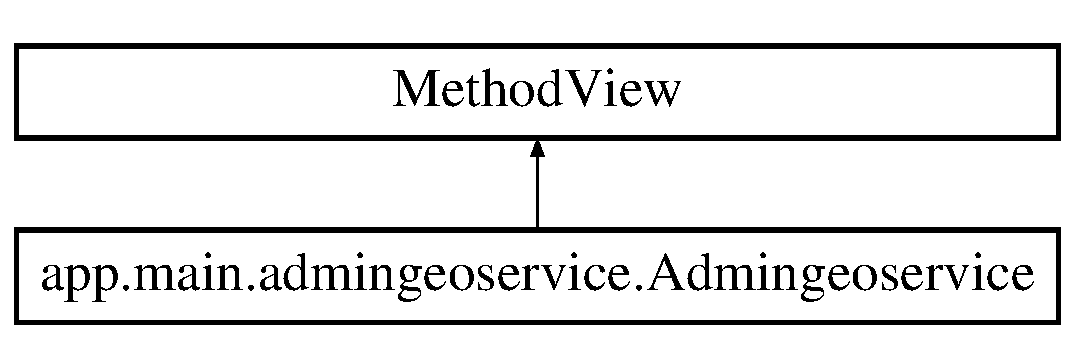
\includegraphics[height=2.000000cm]{classapp_1_1main_1_1admingeoservice_1_1Admingeoservice}
\end{center}
\end{figure}
\subsection*{Static Public Attributes}
\begin{DoxyCompactItemize}
\item 
list {\bfseries yoptlist}
\end{DoxyCompactItemize}


\subsection{Member Data Documentation}
\mbox{\Hypertarget{classapp_1_1main_1_1admingeoservice_1_1Admingeoservice_a7fcc9805c0e5bcbf6306a1db17883264}\label{classapp_1_1main_1_1admingeoservice_1_1Admingeoservice_a7fcc9805c0e5bcbf6306a1db17883264}} 
\index{app\+::main\+::admingeoservice\+::\+Admingeoservice@{app\+::main\+::admingeoservice\+::\+Admingeoservice}!yoptlist@{yoptlist}}
\index{yoptlist@{yoptlist}!app\+::main\+::admingeoservice\+::\+Admingeoservice@{app\+::main\+::admingeoservice\+::\+Admingeoservice}}
\subsubsection{\texorpdfstring{yoptlist}{yoptlist}}
{\footnotesize\ttfamily list app.\+main.\+admingeoservice.\+Admingeoservice.\+yoptlist\hspace{0.3cm}{\ttfamily [static]}}

{\bfseries Initial value\+:}
\begin{DoxyCode}{0}
\DoxyCodeLine{= [}
\DoxyCodeLine{    definitions.SUBJECT\_MATTER,}
\DoxyCodeLine{    definitions.DOMUS\_SUBJECTCLASSIFICATION,}
\DoxyCodeLine{    definitions.GOVERNANCE}
\DoxyCodeLine{    }
\DoxyCodeLine{    ]}
\end{DoxyCode}


The documentation for this class was generated from the following file\+:\begin{DoxyCompactItemize}
\item 
/home/nlarsson/bbk/python/webdev/museumflask/app/main/\mbox{\hyperlink{admingeoservice_8py}{admingeoservice.\+py}}\end{DoxyCompactItemize}

\hypertarget{classapp_1_1main_1_1views_1_1AppConfiguration}{}\section{app.\+main.\+views.\+App\+Configuration Class Reference}
\label{classapp_1_1main_1_1views_1_1AppConfiguration}\index{app.\+main.\+views.\+App\+Configuration@{app.\+main.\+views.\+App\+Configuration}}
Inheritance diagram for app.\+main.\+views.\+App\+Configuration\+:\begin{figure}[H]
\begin{center}
\leavevmode
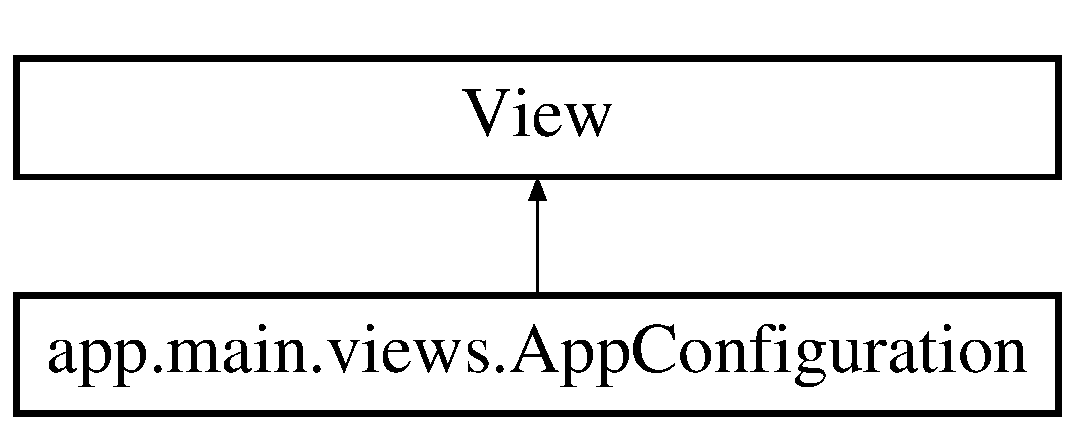
\includegraphics[height=2.000000cm]{classapp_1_1main_1_1views_1_1AppConfiguration}
\end{center}
\end{figure}
\subsection*{Public Member Functions}
\begin{DoxyCompactItemize}
\item 
\mbox{\Hypertarget{classapp_1_1main_1_1views_1_1AppConfiguration_ac382bd938eaeae9ee015eb6db9be4416}\label{classapp_1_1main_1_1views_1_1AppConfiguration_ac382bd938eaeae9ee015eb6db9be4416}} 
def {\bfseries get\+Configuration} (self)
\item 
\mbox{\Hypertarget{classapp_1_1main_1_1views_1_1AppConfiguration_a42b09596ecba29500eba6c491b96e136}\label{classapp_1_1main_1_1views_1_1AppConfiguration_a42b09596ecba29500eba6c491b96e136}} 
def {\bfseries save\+Property} (self, prop, values)
\item 
\mbox{\Hypertarget{classapp_1_1main_1_1views_1_1AppConfiguration_a3bea99e1f7bac0479ab9186252ef3c51}\label{classapp_1_1main_1_1views_1_1AppConfiguration_a3bea99e1f7bac0479ab9186252ef3c51}} 
def {\bfseries reset\+Property} (self, prop)
\item 
\mbox{\Hypertarget{classapp_1_1main_1_1views_1_1AppConfiguration_a614216c4b18ab6556dac3ac23b5f1c75}\label{classapp_1_1main_1_1views_1_1AppConfiguration_a614216c4b18ab6556dac3ac23b5f1c75}} 
def {\bfseries add\+Complementary\+Set\+Non\+Selected} (self, prop, results)
\item 
\mbox{\Hypertarget{classapp_1_1main_1_1views_1_1AppConfiguration_ac1380451be3a057136b4b5fa9ca3b688}\label{classapp_1_1main_1_1views_1_1AppConfiguration_ac1380451be3a057136b4b5fa9ca3b688}} 
def {\bfseries create\+Select\+List} (self, values, reset\+\_\+values)
\item 
\mbox{\Hypertarget{classapp_1_1main_1_1views_1_1AppConfiguration_a8971f657ff05ce067dcbd2bc9b994616}\label{classapp_1_1main_1_1views_1_1AppConfiguration_a8971f657ff05ce067dcbd2bc9b994616}} 
def {\bfseries dispatch\+\_\+request} (self, prop)
\end{DoxyCompactItemize}
\subsection*{Static Public Attributes}
\begin{DoxyCompactItemize}
\item 
\mbox{\Hypertarget{classapp_1_1main_1_1views_1_1AppConfiguration_af16d50d7f35a12e5231e85f3a785301a}\label{classapp_1_1main_1_1views_1_1AppConfiguration_af16d50d7f35a12e5231e85f3a785301a}} 
{\bfseries sel}
\end{DoxyCompactItemize}


The documentation for this class was generated from the following file\+:\begin{DoxyCompactItemize}
\item 
/home/nlarsson/bbk/python/webdev/museumflask/app/main/\mbox{\hyperlink{views_8py}{views.\+py}}\end{DoxyCompactItemize}

\hypertarget{classapp_1_1main_1_1boksplots_1_1bokehcategorybar_1_1BokehCategoryBar}{}\section{app.\+main.\+boksplots.\+bokehcategorybar.\+Bokeh\+Category\+Bar Class Reference}
\label{classapp_1_1main_1_1boksplots_1_1bokehcategorybar_1_1BokehCategoryBar}\index{app.\+main.\+boksplots.\+bokehcategorybar.\+Bokeh\+Category\+Bar@{app.\+main.\+boksplots.\+bokehcategorybar.\+Bokeh\+Category\+Bar}}
\subsection*{Static Public Attributes}
\begin{DoxyCompactItemize}
\item 
\mbox{\Hypertarget{classapp_1_1main_1_1boksplots_1_1bokehcategorybar_1_1BokehCategoryBar_a2cf0f10f86f61e7dd66b1d78f6b209e2}\label{classapp_1_1main_1_1boksplots_1_1bokehcategorybar_1_1BokehCategoryBar_a2cf0f10f86f61e7dd66b1d78f6b209e2}} 
int {\bfseries R\+E\+ST} = 23
\end{DoxyCompactItemize}


The documentation for this class was generated from the following file\+:\begin{DoxyCompactItemize}
\item 
/home/nlarsson/bbk/python/webdev/museumflask/app/main/boksplots/bokehcategorybar.\+py\end{DoxyCompactItemize}

\hypertarget{classapp_1_1main_1_1boksplots_1_1bokehcategorypie_1_1BokehCategoryPie}{}\section{app.\+main.\+boksplots.\+bokehcategorypie.\+Bokeh\+Category\+Pie Class Reference}
\label{classapp_1_1main_1_1boksplots_1_1bokehcategorypie_1_1BokehCategoryPie}\index{app.\+main.\+boksplots.\+bokehcategorypie.\+Bokeh\+Category\+Pie@{app.\+main.\+boksplots.\+bokehcategorypie.\+Bokeh\+Category\+Pie}}
\subsection*{Public Member Functions}
\begin{DoxyCompactItemize}
\item 
\mbox{\Hypertarget{classapp_1_1main_1_1boksplots_1_1bokehcategorypie_1_1BokehCategoryPie_a7086699c3229fd34a3c55ae80896088a}\label{classapp_1_1main_1_1boksplots_1_1bokehcategorypie_1_1BokehCategoryPie_a7086699c3229fd34a3c55ae80896088a}} 
def {\bfseries create\+Plot} (self, me, parameters)
\end{DoxyCompactItemize}
\subsection*{Static Public Member Functions}
\begin{DoxyCompactItemize}
\item 
\mbox{\Hypertarget{classapp_1_1main_1_1boksplots_1_1bokehcategorypie_1_1BokehCategoryPie_a3562537adda021dc755550b2638c3c44}\label{classapp_1_1main_1_1boksplots_1_1bokehcategorypie_1_1BokehCategoryPie_a3562537adda021dc755550b2638c3c44}} 
def {\bfseries get\+Hier\+Data\+Set} (topic, results)
\item 
\mbox{\Hypertarget{classapp_1_1main_1_1boksplots_1_1bokehcategorypie_1_1BokehCategoryPie_a57a3dbe0fd61566f0c64c3201e7cde7e}\label{classapp_1_1main_1_1boksplots_1_1bokehcategorypie_1_1BokehCategoryPie_a57a3dbe0fd61566f0c64c3201e7cde7e}} 
def {\bfseries show\+Pie\+Plot} (topic, results)
\item 
\mbox{\Hypertarget{classapp_1_1main_1_1boksplots_1_1bokehcategorypie_1_1BokehCategoryPie_afc514f480d70bdcc6fa2059ee7550199}\label{classapp_1_1main_1_1boksplots_1_1bokehcategorypie_1_1BokehCategoryPie_afc514f480d70bdcc6fa2059ee7550199}} 
def {\bfseries get\+Pie\+Plot} (score, allscore, classification, counts, rest, tabledict, title, maxval, hovertext)
\end{DoxyCompactItemize}
\subsection*{Static Public Attributes}
\begin{DoxyCompactItemize}
\item 
\mbox{\Hypertarget{classapp_1_1main_1_1boksplots_1_1bokehcategorypie_1_1BokehCategoryPie_ada8481765c445790ca87768097f05895}\label{classapp_1_1main_1_1boksplots_1_1bokehcategorypie_1_1BokehCategoryPie_ada8481765c445790ca87768097f05895}} 
{\bfseries results} = apputils.\+get\+Marker\+Data(props,\mbox{[}bokutils.\+Y\+E\+A\+R\+\_\+\+F\+I\+L\+T\+E\+R3\+\_\+\+O\+P\+EN\mbox{]})
\end{DoxyCompactItemize}


The documentation for this class was generated from the following file\+:\begin{DoxyCompactItemize}
\item 
/home/nlarsson/bbk/python/webdev/museumflask/app/main/boksplots/bokehcategorypie.\+py\end{DoxyCompactItemize}

\hypertarget{classapp_1_1main_1_1boksplots_1_1bokehheatmap_1_1BokehHeatmap}{}\section{app.\+main.\+boksplots.\+bokehheatmap.\+Bokeh\+Heatmap Class Reference}
\label{classapp_1_1main_1_1boksplots_1_1bokehheatmap_1_1BokehHeatmap}\index{app.\+main.\+boksplots.\+bokehheatmap.\+Bokeh\+Heatmap@{app.\+main.\+boksplots.\+bokehheatmap.\+Bokeh\+Heatmap}}
\subsection*{Static Public Attributes}
\begin{DoxyCompactItemize}
\item 
\mbox{\Hypertarget{classapp_1_1main_1_1boksplots_1_1bokehheatmap_1_1BokehHeatmap_a7067a9762c93987006c0cd83ae6636a2}\label{classapp_1_1main_1_1boksplots_1_1bokehheatmap_1_1BokehHeatmap_a7067a9762c93987006c0cd83ae6636a2}} 
string {\bfseries T\+I\+ME} = \char`\"{}Time\char`\"{}
\item 
\mbox{\Hypertarget{classapp_1_1main_1_1boksplots_1_1bokehheatmap_1_1BokehHeatmap_a12c5d9227ec1b35a4d50ed14416f30af}\label{classapp_1_1main_1_1boksplots_1_1bokehheatmap_1_1BokehHeatmap_a12c5d9227ec1b35a4d50ed14416f30af}} 
string {\bfseries Y\+E\+A\+R\+\_\+\+E\+X\+I\+S\+TS} = \textquotesingle{}Year\+\_\+exists\textquotesingle{}
\item 
\mbox{\Hypertarget{classapp_1_1main_1_1boksplots_1_1bokehheatmap_1_1BokehHeatmap_ad5340fe7893e1f24c43afc5008f445db}\label{classapp_1_1main_1_1boksplots_1_1bokehheatmap_1_1BokehHeatmap_ad5340fe7893e1f24c43afc5008f445db}} 
string {\bfseries L\+O\+C\+A\+T\+I\+ON} = \textquotesingle{}Location\textquotesingle{}
\end{DoxyCompactItemize}


The documentation for this class was generated from the following file\+:\begin{DoxyCompactItemize}
\item 
/home/nlarsson/bbk/python/webdev/museumflask/app/main/boksplots/bokehheatmap.\+py\end{DoxyCompactItemize}

\hypertarget{classapp_1_1main_1_1boksplots_1_1bokehtime_1_1BokehTime}{}\section{app.\+main.\+boksplots.\+bokehtime.\+Bokeh\+Time Class Reference}
\label{classapp_1_1main_1_1boksplots_1_1bokehtime_1_1BokehTime}\index{app.\+main.\+boksplots.\+bokehtime.\+Bokeh\+Time@{app.\+main.\+boksplots.\+bokehtime.\+Bokeh\+Time}}
\subsection*{Static Public Attributes}
\begin{DoxyCompactItemize}
\item 
\mbox{\Hypertarget{classapp_1_1main_1_1boksplots_1_1bokehtime_1_1BokehTime_ad7d08589fada4efb5cc216c6d8fa26bc}\label{classapp_1_1main_1_1boksplots_1_1bokehtime_1_1BokehTime_ad7d08589fada4efb5cc216c6d8fa26bc}} 
string {\bfseries T\+I\+ME} = \char`\"{}Time\char`\"{}
\item 
\mbox{\Hypertarget{classapp_1_1main_1_1boksplots_1_1bokehtime_1_1BokehTime_a48ab44982b2cfb074ed10d5410e03ff9}\label{classapp_1_1main_1_1boksplots_1_1bokehtime_1_1BokehTime_a48ab44982b2cfb074ed10d5410e03ff9}} 
string {\bfseries Y\+E\+A\+R\+\_\+\+E\+X\+I\+S\+TS} = \textquotesingle{}Year\+\_\+exists\textquotesingle{}
\end{DoxyCompactItemize}


The documentation for this class was generated from the following file\+:\begin{DoxyCompactItemize}
\item 
/home/nlarsson/bbk/python/webdev/museumflask/app/main/boksplots/bokehtime.\+py\end{DoxyCompactItemize}

\hypertarget{classapp_1_1main_1_1boksplots_1_1bokehtimeandcategory_1_1BokehTimeAndCategory}{}\section{app.\+main.\+boksplots.\+bokehtimeandcategory.\+Bokeh\+Time\+And\+Category Class Reference}
\label{classapp_1_1main_1_1boksplots_1_1bokehtimeandcategory_1_1BokehTimeAndCategory}\index{app.\+main.\+boksplots.\+bokehtimeandcategory.\+Bokeh\+Time\+And\+Category@{app.\+main.\+boksplots.\+bokehtimeandcategory.\+Bokeh\+Time\+And\+Category}}


\subsection{Detailed Description}


 

The documentation for this class was generated from the following file\+:\begin{DoxyCompactItemize}
\item 
/home/nlarsson/bbk/python/webdev/museumflask/app/main/boksplots/bokehtimeandcategory.\+py\end{DoxyCompactItemize}

\hypertarget{classapp_1_1main_1_1boksplots_1_1bokehtree_1_1BokehTree}{}\section{app.\+main.\+boksplots.\+bokehtree.\+Bokeh\+Tree Class Reference}
\label{classapp_1_1main_1_1boksplots_1_1bokehtree_1_1BokehTree}\index{app.\+main.\+boksplots.\+bokehtree.\+Bokeh\+Tree@{app.\+main.\+boksplots.\+bokehtree.\+Bokeh\+Tree}}
\subsection*{Public Member Functions}
\begin{DoxyCompactItemize}
\item 
\mbox{\Hypertarget{classapp_1_1main_1_1boksplots_1_1bokehtree_1_1BokehTree_ab59e84c780a66aea3944cd52b06a527a}\label{classapp_1_1main_1_1boksplots_1_1bokehtree_1_1BokehTree_ab59e84c780a66aea3944cd52b06a527a}} 
def {\bfseries create\+Plot} (self)
\end{DoxyCompactItemize}
\subsection*{Static Public Member Functions}
\begin{DoxyCompactItemize}
\item 
\mbox{\Hypertarget{classapp_1_1main_1_1boksplots_1_1bokehtree_1_1BokehTree_a53243afa451cf8232cdaecb9f50798bc}\label{classapp_1_1main_1_1boksplots_1_1bokehtree_1_1BokehTree_a53243afa451cf8232cdaecb9f50798bc}} 
def {\bfseries normalize\+\_\+sizes} (sizes, dx, dy)
\item 
\mbox{\Hypertarget{classapp_1_1main_1_1boksplots_1_1bokehtree_1_1BokehTree_a3a4378f9e33b16450c274d1b1ab64829}\label{classapp_1_1main_1_1boksplots_1_1bokehtree_1_1BokehTree_a3a4378f9e33b16450c274d1b1ab64829}} 
def {\bfseries layoutrow} (sizes, x, y, dx, dy)
\item 
\mbox{\Hypertarget{classapp_1_1main_1_1boksplots_1_1bokehtree_1_1BokehTree_ae88941c6f46748ab7c1073ae2aa43fe9}\label{classapp_1_1main_1_1boksplots_1_1bokehtree_1_1BokehTree_ae88941c6f46748ab7c1073ae2aa43fe9}} 
def {\bfseries layoutcol} (sizes, x, y, dx, dy)
\item 
\mbox{\Hypertarget{classapp_1_1main_1_1boksplots_1_1bokehtree_1_1BokehTree_a6923d77522db5d51eea89bd4cb810e52}\label{classapp_1_1main_1_1boksplots_1_1bokehtree_1_1BokehTree_a6923d77522db5d51eea89bd4cb810e52}} 
def {\bfseries layout} (sizes, x, y, dx, dy)
\item 
\mbox{\Hypertarget{classapp_1_1main_1_1boksplots_1_1bokehtree_1_1BokehTree_a7fb95025422bc35b8790bf221da4a2c9}\label{classapp_1_1main_1_1boksplots_1_1bokehtree_1_1BokehTree_a7fb95025422bc35b8790bf221da4a2c9}} 
def {\bfseries leftoverrow} (sizes, x, y, dx, dy)
\item 
\mbox{\Hypertarget{classapp_1_1main_1_1boksplots_1_1bokehtree_1_1BokehTree_ad3de5752f26e2349af3322a972a23287}\label{classapp_1_1main_1_1boksplots_1_1bokehtree_1_1BokehTree_ad3de5752f26e2349af3322a972a23287}} 
def {\bfseries leftovercol} (sizes, x, y, dx, dy)
\item 
\mbox{\Hypertarget{classapp_1_1main_1_1boksplots_1_1bokehtree_1_1BokehTree_a8ff1f3a4f7c53b8e79bb3c43ee04dcfd}\label{classapp_1_1main_1_1boksplots_1_1bokehtree_1_1BokehTree_a8ff1f3a4f7c53b8e79bb3c43ee04dcfd}} 
def {\bfseries leftover} (sizes, x, y, dx, dy)
\item 
\mbox{\Hypertarget{classapp_1_1main_1_1boksplots_1_1bokehtree_1_1BokehTree_a9fe84211a581b86dd1e97f122d69d20c}\label{classapp_1_1main_1_1boksplots_1_1bokehtree_1_1BokehTree_a9fe84211a581b86dd1e97f122d69d20c}} 
def {\bfseries worst\+\_\+ratio} (sizes, x, y, dx, dy)
\item 
\mbox{\Hypertarget{classapp_1_1main_1_1boksplots_1_1bokehtree_1_1BokehTree_a221ca3a41008df559308598a4ec2bcd0}\label{classapp_1_1main_1_1boksplots_1_1bokehtree_1_1BokehTree_a221ca3a41008df559308598a4ec2bcd0}} 
def {\bfseries squarify} (sizes, x, y, dx, dy)
\end{DoxyCompactItemize}


The documentation for this class was generated from the following file\+:\begin{DoxyCompactItemize}
\item 
/home/nlarsson/bbk/python/webdev/museumflask/app/main/boksplots/bokehtree.\+py\end{DoxyCompactItemize}

\hypertarget{classapp_1_1main_1_1boks_1_1Boks}{}\section{app.\+main.\+boks.\+Boks Class Reference}
\label{classapp_1_1main_1_1boks_1_1Boks}\index{app.\+main.\+boks.\+Boks@{app.\+main.\+boks.\+Boks}}
\subsection*{Classes}
\begin{DoxyCompactItemize}
\item 
class \mbox{\hyperlink{classapp_1_1main_1_1boks_1_1Boks_1_1closings__over__time}{closings\+\_\+over\+\_\+time}}
\item 
class \mbox{\hyperlink{classapp_1_1main_1_1boks_1_1Boks_1_1open__at__a__given__time}{open\+\_\+at\+\_\+a\+\_\+given\+\_\+time}}
\item 
class \mbox{\hyperlink{classapp_1_1main_1_1boks_1_1Boks_1_1open__over__time}{open\+\_\+over\+\_\+time}}
\item 
class \mbox{\hyperlink{classapp_1_1main_1_1boks_1_1Boks_1_1openings__and__closings__over__time}{openings\+\_\+and\+\_\+closings\+\_\+over\+\_\+time}}
\item 
class \mbox{\hyperlink{classapp_1_1main_1_1boks_1_1Boks_1_1openings__over__time}{openings\+\_\+over\+\_\+time}}
\item 
class \mbox{\hyperlink{classapp_1_1main_1_1boks_1_1Boks_1_1test__of__heatmap}{test\+\_\+of\+\_\+heatmap}}
\item 
class \mbox{\hyperlink{classapp_1_1main_1_1boks_1_1Boks_1_1that__opened__up__to__a__given__time}{that\+\_\+opened\+\_\+up\+\_\+to\+\_\+a\+\_\+given\+\_\+time}}
\end{DoxyCompactItemize}
\subsection*{Static Public Attributes}
\begin{DoxyCompactItemize}
\item 
list \mbox{\hyperlink{classapp_1_1main_1_1boks_1_1Boks_a50e069a721957bccdb1841d00d19d954}{timelist}}
\begin{DoxyCompactList}\small\item\em Menu structure. \end{DoxyCompactList}\item 
list \mbox{\hyperlink{classapp_1_1main_1_1boks_1_1Boks_a9fca61dce81ef716bbe04922482878c8}{heatmapoptions}}
\begin{DoxyCompactList}\small\item\em Query options. \end{DoxyCompactList}\item 
\mbox{\Hypertarget{classapp_1_1main_1_1boks_1_1Boks_a85a671e45aacb497475936c3834ed235}\label{classapp_1_1main_1_1boks_1_1Boks_a85a671e45aacb497475936c3834ed235}} 
string {\bfseries U\+K\+N\+A\+ME} = \char`\"{}UK\char`\"{}
\item 
\mbox{\Hypertarget{classapp_1_1main_1_1boks_1_1Boks_ac8f4e6d848c3cf4f4b8a2f99e08562fc}\label{classapp_1_1main_1_1boks_1_1Boks_ac8f4e6d848c3cf4f4b8a2f99e08562fc}} 
string {\bfseries N\+Ogreeting} = \char`\"{}Hello\char`\"{}
\item 
\mbox{\Hypertarget{classapp_1_1main_1_1boks_1_1Boks_ad67863bfb4abf4cd1cee174560f7a335}\label{classapp_1_1main_1_1boks_1_1Boks_ad67863bfb4abf4cd1cee174560f7a335}} 
{\bfseries greeting} = None
\item 
\mbox{\Hypertarget{classapp_1_1main_1_1boks_1_1Boks_a4d8258f46426c6b9d264e60b7a93fd02}\label{classapp_1_1main_1_1boks_1_1Boks_a4d8258f46426c6b9d264e60b7a93fd02}} 
{\bfseries btree}
\item 
\mbox{\Hypertarget{classapp_1_1main_1_1boks_1_1Boks_aea3f7421879503580c22b8e3e6c40bfe}\label{classapp_1_1main_1_1boks_1_1Boks_aea3f7421879503580c22b8e3e6c40bfe}} 
{\bfseries timeandcategory} = bokehtimeandcategory.\+Bokeh\+Time\+And\+Category()
\item 
\mbox{\Hypertarget{classapp_1_1main_1_1boks_1_1Boks_ada877ef3ee5a0d6f26f30699a594244c}\label{classapp_1_1main_1_1boks_1_1Boks_ada877ef3ee5a0d6f26f30699a594244c}} 
{\bfseries time} = bokehtime.\+Bokeh\+Time()
\item 
\mbox{\Hypertarget{classapp_1_1main_1_1boks_1_1Boks_adb071826a4e1d3632061509c98ecfd4e}\label{classapp_1_1main_1_1boks_1_1Boks_adb071826a4e1d3632061509c98ecfd4e}} 
{\bfseries categorybar} = bokehcategorybar.\+Bokeh\+Category\+Bar()
\item 
\mbox{\Hypertarget{classapp_1_1main_1_1boks_1_1Boks_acf295f36cfe7ceb99a049fd7bbab840d}\label{classapp_1_1main_1_1boks_1_1Boks_acf295f36cfe7ceb99a049fd7bbab840d}} 
{\bfseries heat} = bokehheatmap.\+Bokeh\+Heatmap()
\item 
\mbox{\Hypertarget{classapp_1_1main_1_1boks_1_1Boks_ae1094117f1478a1e543996e04f375784}\label{classapp_1_1main_1_1boks_1_1Boks_ae1094117f1478a1e543996e04f375784}} 
string {\bfseries greeting} = \textquotesingle{}\textquotesingle{}.join(greeting).replace(\char`\"{}\textbackslash{}n\char`\"{},\char`\"{}\char`\"{})
\item 
\mbox{\Hypertarget{classapp_1_1main_1_1boks_1_1Boks_a8245b3488e844577628fd279e1eb83d9}\label{classapp_1_1main_1_1boks_1_1Boks_a8245b3488e844577628fd279e1eb83d9}} 
{\bfseries menucoltree} = None
\item 
\mbox{\Hypertarget{classapp_1_1main_1_1boks_1_1Boks_a583153e3fc5a2e3aa7d8a3a590107b4e}\label{classapp_1_1main_1_1boks_1_1Boks_a583153e3fc5a2e3aa7d8a3a590107b4e}} 
{\bfseries menuxtree} = None
\item 
\mbox{\Hypertarget{classapp_1_1main_1_1boks_1_1Boks_a044312bc393249e64e708c2d8a51adf8}\label{classapp_1_1main_1_1boks_1_1Boks_a044312bc393249e64e708c2d8a51adf8}} 
{\bfseries menuytree} = None
\item 
\mbox{\Hypertarget{classapp_1_1main_1_1boks_1_1Boks_a7a9ef5a0f2412ef57784799f5af2c72f}\label{classapp_1_1main_1_1boks_1_1Boks_a7a9ef5a0f2412ef57784799f5af2c72f}} 
{\bfseries menutree} = None
\item 
\mbox{\Hypertarget{classapp_1_1main_1_1boks_1_1Boks_a8b3e81c3cfae68f3f8fa6dbd134a6829}\label{classapp_1_1main_1_1boks_1_1Boks_a8b3e81c3cfae68f3f8fa6dbd134a6829}} 
{\bfseries locatree} = None
\item 
\mbox{\Hypertarget{classapp_1_1main_1_1boks_1_1Boks_acdc85a52a609e34907e91eab32539af7}\label{classapp_1_1main_1_1boks_1_1Boks_acdc85a52a609e34907e91eab32539af7}} 
{\bfseries locnode} = None
\item 
\mbox{\Hypertarget{classapp_1_1main_1_1boks_1_1Boks_a56f4d3de4ff53aad85dcb9069eb310a9}\label{classapp_1_1main_1_1boks_1_1Boks_a56f4d3de4ff53aad85dcb9069eb310a9}} 
{\bfseries menut} = None
\end{DoxyCompactItemize}


\subsection{Member Data Documentation}
\mbox{\Hypertarget{classapp_1_1main_1_1boks_1_1Boks_a9fca61dce81ef716bbe04922482878c8}\label{classapp_1_1main_1_1boks_1_1Boks_a9fca61dce81ef716bbe04922482878c8}} 
\index{app\+::main\+::boks\+::\+Boks@{app\+::main\+::boks\+::\+Boks}!heatmapoptions@{heatmapoptions}}
\index{heatmapoptions@{heatmapoptions}!app\+::main\+::boks\+::\+Boks@{app\+::main\+::boks\+::\+Boks}}
\subsubsection{\texorpdfstring{heatmapoptions}{heatmapoptions}}
{\footnotesize\ttfamily list app.\+main.\+boks.\+Boks.\+heatmapoptions\hspace{0.3cm}{\ttfamily [static]}}

{\bfseries Initial value\+:}
\begin{DoxyCode}{0}
\DoxyCodeLine{= [}
\DoxyCodeLine{    definitions.GOVERNANCE,}
\DoxyCodeLine{    definitions.SUBJECT\_MATTER,}
\DoxyCodeLine{    definitions.SIZE,}
\DoxyCodeLine{    \textcolor{stringliteral}{"Location"}}
\DoxyCodeLine{    ]}
\end{DoxyCode}


Query options. 

\mbox{\Hypertarget{classapp_1_1main_1_1boks_1_1Boks_a50e069a721957bccdb1841d00d19d954}\label{classapp_1_1main_1_1boks_1_1Boks_a50e069a721957bccdb1841d00d19d954}} 
\index{app\+::main\+::boks\+::\+Boks@{app\+::main\+::boks\+::\+Boks}!timelist@{timelist}}
\index{timelist@{timelist}!app\+::main\+::boks\+::\+Boks@{app\+::main\+::boks\+::\+Boks}}
\subsubsection{\texorpdfstring{timelist}{timelist}}
{\footnotesize\ttfamily list app.\+main.\+boks.\+Boks.\+timelist\hspace{0.3cm}{\ttfamily [static]}}

{\bfseries Initial value\+:}
\begin{DoxyCode}{0}
\DoxyCodeLine{= [}
\DoxyCodeLine{    \textcolor{stringliteral}{"open at a given time"},}
\DoxyCodeLine{    \textcolor{stringliteral}{"that opened up to a given time"},}
\DoxyCodeLine{    \textcolor{stringliteral}{"open over time"},}
\DoxyCodeLine{    \textcolor{stringliteral}{"openings over time"},}
\DoxyCodeLine{    \textcolor{stringliteral}{"closings over time"}}
\DoxyCodeLine{    ]}
\end{DoxyCode}


Menu structure. 



The documentation for this class was generated from the following file\+:\begin{DoxyCompactItemize}
\item 
/home/nlarsson/bbk/python/webdev/museumflask/app/main/\mbox{\hyperlink{boks_8py}{boks.\+py}}\end{DoxyCompactItemize}

\hypertarget{classapp_1_1main_1_1chloro_1_1Chloro}{}\section{app.\+main.\+chloro.\+Chloro Class Reference}
\label{classapp_1_1main_1_1chloro_1_1Chloro}\index{app.\+main.\+chloro.\+Chloro@{app.\+main.\+chloro.\+Chloro}}
\subsection*{Static Public Attributes}
\begin{DoxyCompactItemize}
\item 
\mbox{\Hypertarget{classapp_1_1main_1_1chloro_1_1Chloro_a895a373a54e52b3ebdcfd70ac36a5b17}\label{classapp_1_1main_1_1chloro_1_1Chloro_a895a373a54e52b3ebdcfd70ac36a5b17}} 
{\bfseries mapchart} = \mbox{\hyperlink{classapp_1_1main_1_1mapchart_1_1MapChart}{mapchart.\+Map\+Chart}}()
\end{DoxyCompactItemize}


The documentation for this class was generated from the following file\+:\begin{DoxyCompactItemize}
\item 
/home/nlarsson/bbk/python/webdev/museumflask/app/main/\mbox{\hyperlink{chloro_8py}{chloro.\+py}}\end{DoxyCompactItemize}

\hypertarget{classapp_1_1main_1_1boks_1_1Boks_1_1closings__over__time}{}\section{app.\+main.\+boks.\+Boks.\+closings\+\_\+over\+\_\+time Class Reference}
\label{classapp_1_1main_1_1boks_1_1Boks_1_1closings__over__time}\index{app.\+main.\+boks.\+Boks.\+closings\+\_\+over\+\_\+time@{app.\+main.\+boks.\+Boks.\+closings\+\_\+over\+\_\+time}}
\subsection*{Public Member Functions}
\begin{DoxyCompactItemize}
\item 
\mbox{\Hypertarget{classapp_1_1main_1_1boks_1_1Boks_1_1closings__over__time_a1a99c27f7d0845930fe706ad26cc3fb3}\label{classapp_1_1main_1_1boks_1_1Boks_1_1closings__over__time_a1a99c27f7d0845930fe706ad26cc3fb3}} 
def {\bfseries Governance} (self, me, parameters=None, contextdict=None)
\item 
\mbox{\Hypertarget{classapp_1_1main_1_1boks_1_1Boks_1_1closings__over__time_a359d58dc14b277e2ecf92a17411f3d36}\label{classapp_1_1main_1_1boks_1_1Boks_1_1closings__over__time_a359d58dc14b277e2ecf92a17411f3d36}} 
def {\bfseries Subject\+\_\+\+Matter} (self, me, parameters=None, contextdict=None)
\item 
\mbox{\Hypertarget{classapp_1_1main_1_1boks_1_1Boks_1_1closings__over__time_a2e4912e28a19b26b9cfd28f87f56fcfa}\label{classapp_1_1main_1_1boks_1_1Boks_1_1closings__over__time_a2e4912e28a19b26b9cfd28f87f56fcfa}} 
def {\bfseries Size} (self, me, parameters=None, contextdict=None)
\item 
\mbox{\Hypertarget{classapp_1_1main_1_1boks_1_1Boks_1_1closings__over__time_a25878330624e2b58af9d22b051943739}\label{classapp_1_1main_1_1boks_1_1Boks_1_1closings__over__time_a25878330624e2b58af9d22b051943739}} 
def {\bfseries All} (self, me, parameters=None, contextdict=None)
\item 
\mbox{\Hypertarget{classapp_1_1main_1_1boks_1_1Boks_1_1closings__over__time_aec35ba8ffdcc2bb52986a04012808a07}\label{classapp_1_1main_1_1boks_1_1Boks_1_1closings__over__time_aec35ba8ffdcc2bb52986a04012808a07}} 
def {\bfseries Location} (self, me, parameters=None, contextdict=None)
\end{DoxyCompactItemize}
\subsection*{Static Public Attributes}
\begin{DoxyCompactItemize}
\item 
\mbox{\Hypertarget{classapp_1_1main_1_1boks_1_1Boks_1_1closings__over__time_abcc4150c2384a45d5200e3d529c69da5}\label{classapp_1_1main_1_1boks_1_1Boks_1_1closings__over__time_abcc4150c2384a45d5200e3d529c69da5}} 
{\bfseries plot} = Boks.\+timeandcategory.\+create\+Location\+Plot(\char`\"{}location\char`\"{},newparameters,contextdict)
\end{DoxyCompactItemize}


The documentation for this class was generated from the following file\+:\begin{DoxyCompactItemize}
\item 
/home/nlarsson/bbk/python/webdev/museumflask/app/main/\mbox{\hyperlink{boks_8py}{boks.\+py}}\end{DoxyCompactItemize}

\hypertarget{classapp_1_1main_1_1Configuration_1_1Configuration}{}\section{app.\+main.\+Configuration.\+Configuration Class Reference}
\label{classapp_1_1main_1_1Configuration_1_1Configuration}\index{app.\+main.\+Configuration.\+Configuration@{app.\+main.\+Configuration.\+Configuration}}
\subsection*{Public Member Functions}
\begin{DoxyCompactItemize}
\item 
\mbox{\Hypertarget{classapp_1_1main_1_1Configuration_1_1Configuration_a90448d977ae02bd04ff9402505023379}\label{classapp_1_1main_1_1Configuration_1_1Configuration_a90448d977ae02bd04ff9402505023379}} 
def {\bfseries \+\_\+\+\_\+init\+\_\+\+\_\+} (self, configs=\{\}, name=None)
\item 
\mbox{\Hypertarget{classapp_1_1main_1_1Configuration_1_1Configuration_a75a3867cdeddaeb94aca37c22b8e25a0}\label{classapp_1_1main_1_1Configuration_1_1Configuration_a75a3867cdeddaeb94aca37c22b8e25a0}} 
def {\bfseries set} (self, key, value)
\item 
\mbox{\Hypertarget{classapp_1_1main_1_1Configuration_1_1Configuration_a747bdc4ecfdc71dd7772c5e493781b83}\label{classapp_1_1main_1_1Configuration_1_1Configuration_a747bdc4ecfdc71dd7772c5e493781b83}} 
def {\bfseries get} (self, key)
\item 
\mbox{\Hypertarget{classapp_1_1main_1_1Configuration_1_1Configuration_aa265be67d3514a54b09703dffc2114d2}\label{classapp_1_1main_1_1Configuration_1_1Configuration_aa265be67d3514a54b09703dffc2114d2}} 
def {\bfseries print\+Key} (self, key)
\item 
\mbox{\Hypertarget{classapp_1_1main_1_1Configuration_1_1Configuration_a7bf71df11d28da7f7ce62e9c40f014e9}\label{classapp_1_1main_1_1Configuration_1_1Configuration_a7bf71df11d28da7f7ce62e9c40f014e9}} 
def {\bfseries save} (self)
\item 
\mbox{\Hypertarget{classapp_1_1main_1_1Configuration_1_1Configuration_a79f4a29c1589c00e513ab6dae52363ec}\label{classapp_1_1main_1_1Configuration_1_1Configuration_a79f4a29c1589c00e513ab6dae52363ec}} 
def {\bfseries load} (self)
\end{DoxyCompactItemize}
\subsection*{Public Attributes}
\begin{DoxyCompactItemize}
\item 
\mbox{\Hypertarget{classapp_1_1main_1_1Configuration_1_1Configuration_a3b90253c8b5b66e2060b563cbc60a057}\label{classapp_1_1main_1_1Configuration_1_1Configuration_a3b90253c8b5b66e2060b563cbc60a057}} 
{\bfseries config}
\item 
\mbox{\Hypertarget{classapp_1_1main_1_1Configuration_1_1Configuration_a2b24039b120353f6566b42bdc4d57d43}\label{classapp_1_1main_1_1Configuration_1_1Configuration_a2b24039b120353f6566b42bdc4d57d43}} 
{\bfseries name}
\item 
\mbox{\Hypertarget{classapp_1_1main_1_1Configuration_1_1Configuration_ab3093a6a604a575dd05b49eb067be029}\label{classapp_1_1main_1_1Configuration_1_1Configuration_ab3093a6a604a575dd05b49eb067be029}} 
{\bfseries dict}
\end{DoxyCompactItemize}
\subsection*{Static Public Attributes}
\begin{DoxyCompactItemize}
\item 
\mbox{\Hypertarget{classapp_1_1main_1_1Configuration_1_1Configuration_a18ad426c4d3dba204c19dc70e94a5566}\label{classapp_1_1main_1_1Configuration_1_1Configuration_a18ad426c4d3dba204c19dc70e94a5566}} 
string {\bfseries D\+A\+T\+A\+\_\+\+P\+TR} = \textquotesingle{}D\+A\+TA\textquotesingle{}
\item 
\mbox{\Hypertarget{classapp_1_1main_1_1Configuration_1_1Configuration_a7b2b4dfd578c07ae14e3d5a30f66371a}\label{classapp_1_1main_1_1Configuration_1_1Configuration_a7b2b4dfd578c07ae14e3d5a30f66371a}} 
string {\bfseries T\+Y\+P\+E\+\_\+\+P\+TR} = \textquotesingle{}D\+A\+T\+A\+T\+Y\+PE\textquotesingle{}
\item 
\mbox{\Hypertarget{classapp_1_1main_1_1Configuration_1_1Configuration_a9d35d0bdf2a22fdf4cbf009b593a5699}\label{classapp_1_1main_1_1Configuration_1_1Configuration_a9d35d0bdf2a22fdf4cbf009b593a5699}} 
string {\bfseries O\+P\+T\+I\+O\+N\+S\+\_\+\+P\+TR} = \textquotesingle{}O\+P\+T\+I\+O\+NS\textquotesingle{}
\end{DoxyCompactItemize}


The documentation for this class was generated from the following file\+:\begin{DoxyCompactItemize}
\item 
/home/nlarsson/bbk/python/webdev/museumflask/app/main/\mbox{\hyperlink{Configuration_8py}{Configuration.\+py}}\end{DoxyCompactItemize}

\hypertarget{classapp_1_1main_1_1boksplots_1_1custompie_1_1CustomPieBuilder}{}\section{app.\+main.\+boksplots.\+custompie.\+Custom\+Pie\+Builder Class Reference}
\label{classapp_1_1main_1_1boksplots_1_1custompie_1_1CustomPieBuilder}\index{app.\+main.\+boksplots.\+custompie.\+Custom\+Pie\+Builder@{app.\+main.\+boksplots.\+custompie.\+Custom\+Pie\+Builder}}
\subsection*{Public Member Functions}
\begin{DoxyCompactItemize}
\item 
\mbox{\Hypertarget{classapp_1_1main_1_1boksplots_1_1custompie_1_1CustomPieBuilder_ad2496bea2b724544cc91c3eb08852262}\label{classapp_1_1main_1_1boksplots_1_1custompie_1_1CustomPieBuilder_ad2496bea2b724544cc91c3eb08852262}} 
def {\bfseries \+\_\+\+\_\+init\+\_\+\+\_\+} (self, df, label\+\_\+name, column\+\_\+name, tools=\textquotesingle{}hover\textquotesingle{}, tooltips=None, reverse\+\_\+color=False, colors=None, random\+\_\+color\+\_\+order=False, plot\+\_\+width=bokutils.\+P\+L\+O\+T\+\_\+\+W\+I\+D\+TH, plot\+\_\+height=bokutils.\+P\+L\+O\+T\+\_\+\+H\+E\+I\+G\+HT, title=\textquotesingle{}Untitled\textquotesingle{}, args, kwargs)
\item 
\mbox{\Hypertarget{classapp_1_1main_1_1boksplots_1_1custompie_1_1CustomPieBuilder_abc5606033b421af199fea19d4a587d28}\label{classapp_1_1main_1_1boksplots_1_1custompie_1_1CustomPieBuilder_abc5606033b421af199fea19d4a587d28}} 
def {\bfseries setup\+\_\+figure} (self, tools, plot\+\_\+width, plot\+\_\+height, title)
\end{DoxyCompactItemize}
\subsection*{Static Public Member Functions}
\begin{DoxyCompactItemize}
\item 
\mbox{\Hypertarget{classapp_1_1main_1_1boksplots_1_1custompie_1_1CustomPieBuilder_af0edef2b36a14326bdf87afe5d652035}\label{classapp_1_1main_1_1boksplots_1_1custompie_1_1CustomPieBuilder_af0edef2b36a14326bdf87afe5d652035}} 
def {\bfseries plot\+\_\+pie} (p, df, label\+\_\+name, args, kwargs)
\item 
\mbox{\Hypertarget{classapp_1_1main_1_1boksplots_1_1custompie_1_1CustomPieBuilder_ab710a02880adebb9173a1bb67bc0a5b3}\label{classapp_1_1main_1_1boksplots_1_1custompie_1_1CustomPieBuilder_ab710a02880adebb9173a1bb67bc0a5b3}} 
def {\bfseries set\+\_\+hover\+\_\+tooltip} (p, tooltips)
\item 
\mbox{\Hypertarget{classapp_1_1main_1_1boksplots_1_1custompie_1_1CustomPieBuilder_abc69d564224c99c2c0f66d28d85d66e1}\label{classapp_1_1main_1_1boksplots_1_1custompie_1_1CustomPieBuilder_abc69d564224c99c2c0f66d28d85d66e1}} 
def {\bfseries add\+\_\+columns\+\_\+for\+\_\+pie\+\_\+chart} (df, column\+\_\+name, colors=None, reverse\+\_\+color=False, random\+\_\+color\+\_\+order=False)
\item 
\mbox{\Hypertarget{classapp_1_1main_1_1boksplots_1_1custompie_1_1CustomPieBuilder_a16ec42edb5251960fd6abadd7728f3da}\label{classapp_1_1main_1_1boksplots_1_1custompie_1_1CustomPieBuilder_a16ec42edb5251960fd6abadd7728f3da}} 
def {\bfseries add\+\_\+text\+\_\+label\+\_\+on\+\_\+pie} (p, df, label\+\_\+name)
\end{DoxyCompactItemize}
\subsection*{Public Attributes}
\begin{DoxyCompactItemize}
\item 
\mbox{\Hypertarget{classapp_1_1main_1_1boksplots_1_1custompie_1_1CustomPieBuilder_a794192b13af422ca19c0a017dd308eca}\label{classapp_1_1main_1_1boksplots_1_1custompie_1_1CustomPieBuilder_a794192b13af422ca19c0a017dd308eca}} 
{\bfseries df}
\item 
\mbox{\Hypertarget{classapp_1_1main_1_1boksplots_1_1custompie_1_1CustomPieBuilder_a1dd0197d210d923d64452d885debbce3}\label{classapp_1_1main_1_1boksplots_1_1custompie_1_1CustomPieBuilder_a1dd0197d210d923d64452d885debbce3}} 
{\bfseries plot}
\end{DoxyCompactItemize}
\subsection*{Static Public Attributes}
\begin{DoxyCompactItemize}
\item 
\mbox{\Hypertarget{classapp_1_1main_1_1boksplots_1_1custompie_1_1CustomPieBuilder_a37ff9d2647081d878e0f08febc66b9be}\label{classapp_1_1main_1_1boksplots_1_1custompie_1_1CustomPieBuilder_a37ff9d2647081d878e0f08febc66b9be}} 
string {\bfseries green} = \char`\"{}\#50ee70\char`\"{}
\item 
\mbox{\Hypertarget{classapp_1_1main_1_1boksplots_1_1custompie_1_1CustomPieBuilder_a8014d4ebb12a2c910a7ca9b3cb6aa76b}\label{classapp_1_1main_1_1boksplots_1_1custompie_1_1CustomPieBuilder_a8014d4ebb12a2c910a7ca9b3cb6aa76b}} 
string {\bfseries red} = \char`\"{}\#ff7070\char`\"{}
\item 
\mbox{\Hypertarget{classapp_1_1main_1_1boksplots_1_1custompie_1_1CustomPieBuilder_aa07629eb8f7591d1e06ebd0a1b98ed40}\label{classapp_1_1main_1_1boksplots_1_1custompie_1_1CustomPieBuilder_aa07629eb8f7591d1e06ebd0a1b98ed40}} 
float {\bfseries x\+\_\+range} = 1.\+1
\item 
\mbox{\Hypertarget{classapp_1_1main_1_1boksplots_1_1custompie_1_1CustomPieBuilder_acbab538280eb6d196e63a9ddc7b4daec}\label{classapp_1_1main_1_1boksplots_1_1custompie_1_1CustomPieBuilder_acbab538280eb6d196e63a9ddc7b4daec}} 
float {\bfseries y\+\_\+range} = 1.\+1
\end{DoxyCompactItemize}


The documentation for this class was generated from the following file\+:\begin{DoxyCompactItemize}
\item 
/home/nlarsson/bbk/python/webdev/museumflask/app/main/boksplots/custompie.\+py\end{DoxyCompactItemize}

\hypertarget{classapp_1_1main_1_1datasetversionservice_1_1Datasetversionservice}{}\section{app.\+main.\+datasetversionservice.\+Datasetversionservice Class Reference}
\label{classapp_1_1main_1_1datasetversionservice_1_1Datasetversionservice}\index{app.\+main.\+datasetversionservice.\+Datasetversionservice@{app.\+main.\+datasetversionservice.\+Datasetversionservice}}
Inheritance diagram for app.\+main.\+datasetversionservice.\+Datasetversionservice\+:\begin{figure}[H]
\begin{center}
\leavevmode
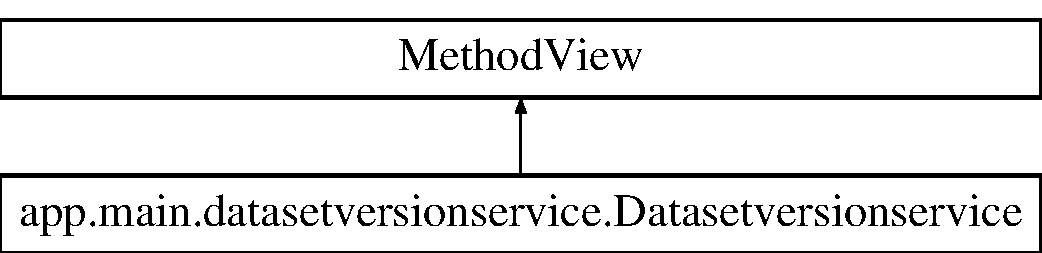
\includegraphics[height=2.000000cm]{classapp_1_1main_1_1datasetversionservice_1_1Datasetversionservice}
\end{center}
\end{figure}
\subsection*{Static Public Attributes}
\begin{DoxyCompactItemize}
\item 
\mbox{\Hypertarget{classapp_1_1main_1_1datasetversionservice_1_1Datasetversionservice_aad5d55559fef770b6bac27042903cff2}\label{classapp_1_1main_1_1datasetversionservice_1_1Datasetversionservice_aad5d55559fef770b6bac27042903cff2}} 
{\bfseries V\+E\+R\+S\+I\+ON} = None
\end{DoxyCompactItemize}


The documentation for this class was generated from the following file\+:\begin{DoxyCompactItemize}
\item 
/home/nlarsson/bbk/python/webdev/museumflask/app/main/\mbox{\hyperlink{datasetversionservice_8py}{datasetversionservice.\+py}}\end{DoxyCompactItemize}

\hypertarget{classapp_1_1main_1_1treelib_1_1exceptions_1_1DuplicatedNodeIdError}{}\section{app.\+main.\+treelib.\+exceptions.\+Duplicated\+Node\+Id\+Error Class Reference}
\label{classapp_1_1main_1_1treelib_1_1exceptions_1_1DuplicatedNodeIdError}\index{app.\+main.\+treelib.\+exceptions.\+Duplicated\+Node\+Id\+Error@{app.\+main.\+treelib.\+exceptions.\+Duplicated\+Node\+Id\+Error}}
Inheritance diagram for app.\+main.\+treelib.\+exceptions.\+Duplicated\+Node\+Id\+Error\+:\begin{figure}[H]
\begin{center}
\leavevmode
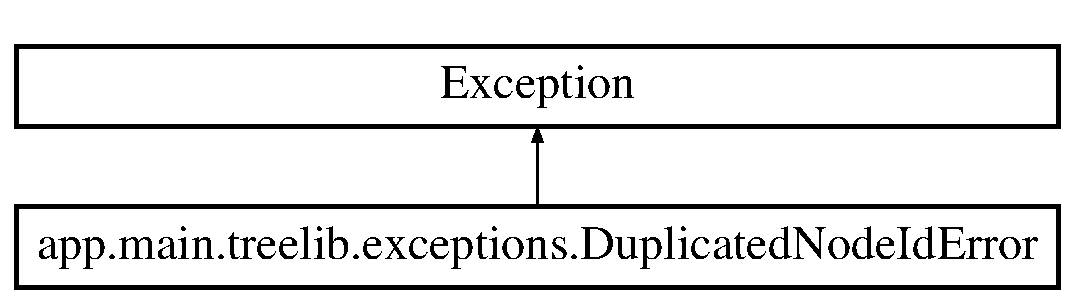
\includegraphics[height=2.000000cm]{classapp_1_1main_1_1treelib_1_1exceptions_1_1DuplicatedNodeIdError}
\end{center}
\end{figure}


\subsection{Detailed Description}
\begin{DoxyVerb}Exception throwed if an identifier already exists in a tree.\end{DoxyVerb}
 

The documentation for this class was generated from the following file\+:\begin{DoxyCompactItemize}
\item 
/home/nlarsson/bbk/python/webdev/museumflask/app/main/treelib/exceptions.\+py\end{DoxyCompactItemize}

\hypertarget{classapp_1_1main_1_1datatypes_1_1Governance__Change_1_1Governance__Change}{}\section{app.\+main.\+datatypes.\+Governance\+\_\+\+Change.\+Governance\+\_\+\+Change Class Reference}
\label{classapp_1_1main_1_1datatypes_1_1Governance__Change_1_1Governance__Change}\index{app.\+main.\+datatypes.\+Governance\+\_\+\+Change.\+Governance\+\_\+\+Change@{app.\+main.\+datatypes.\+Governance\+\_\+\+Change.\+Governance\+\_\+\+Change}}
Inheritance diagram for app.\+main.\+datatypes.\+Governance\+\_\+\+Change.\+Governance\+\_\+\+Change\+:\begin{figure}[H]
\begin{center}
\leavevmode
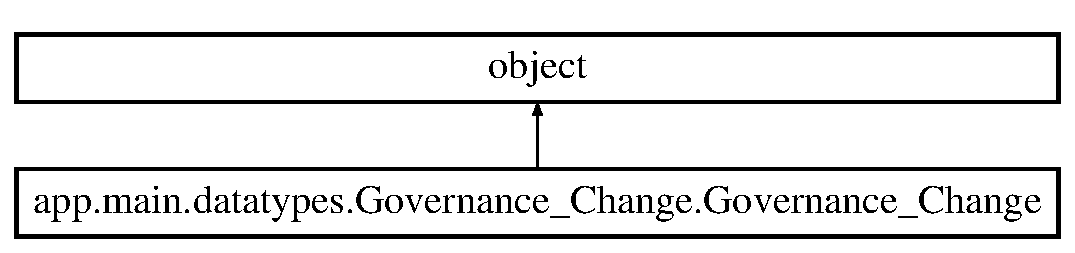
\includegraphics[height=2.000000cm]{classapp_1_1main_1_1datatypes_1_1Governance__Change_1_1Governance__Change}
\end{center}
\end{figure}
\subsection*{Public Member Functions}
\begin{DoxyCompactItemize}
\item 
\mbox{\Hypertarget{classapp_1_1main_1_1datatypes_1_1Governance__Change_1_1Governance__Change_a9ba7afb2644887d7ac3eb49e3a0b8a94}\label{classapp_1_1main_1_1datatypes_1_1Governance__Change_1_1Governance__Change_a9ba7afb2644887d7ac3eb49e3a0b8a94}} 
def {\bfseries \+\_\+\+\_\+init\+\_\+\+\_\+} (self)
\item 
\mbox{\Hypertarget{classapp_1_1main_1_1datatypes_1_1Governance__Change_1_1Governance__Change_a3933ab27c83521ccb7103c1785800abe}\label{classapp_1_1main_1_1datatypes_1_1Governance__Change_1_1Governance__Change_a3933ab27c83521ccb7103c1785800abe}} 
def {\bfseries get\+Match\+Filter} (self, rcount, match, condition)
\item 
\mbox{\Hypertarget{classapp_1_1main_1_1datatypes_1_1Governance__Change_1_1Governance__Change_a85c7dcec827be73d2d1a946df8992d82}\label{classapp_1_1main_1_1datatypes_1_1Governance__Change_1_1Governance__Change_a85c7dcec827be73d2d1a946df8992d82}} 
def {\bfseries get\+Compare\+Filter} (self, rcount, match, condition)
\item 
\mbox{\Hypertarget{classapp_1_1main_1_1datatypes_1_1Governance__Change_1_1Governance__Change_a65cda2045613958068803849697189f2}\label{classapp_1_1main_1_1datatypes_1_1Governance__Change_1_1Governance__Change_a65cda2045613958068803849697189f2}} 
def {\bfseries get\+Query} (self, col, rcount, matchstring, condition, matchcolumn)
\item 
\mbox{\Hypertarget{classapp_1_1main_1_1datatypes_1_1Governance__Change_1_1Governance__Change_a34827a839e393a116ea8e32193b45193}\label{classapp_1_1main_1_1datatypes_1_1Governance__Change_1_1Governance__Change_a34827a839e393a116ea8e32193b45193}} 
def {\bfseries get\+Search\+Type} (self)
\item 
\mbox{\Hypertarget{classapp_1_1main_1_1datatypes_1_1Governance__Change_1_1Governance__Change_a1025a0713329a2e7e12f24f935915c92}\label{classapp_1_1main_1_1datatypes_1_1Governance__Change_1_1Governance__Change_a1025a0713329a2e7e12f24f935915c92}} 
def {\bfseries get\+G\+U\+I\+Conditions} (self)
\item 
\mbox{\Hypertarget{classapp_1_1main_1_1datatypes_1_1Governance__Change_1_1Governance__Change_ad9306a06f912b64577b6887bd0cd4fdb}\label{classapp_1_1main_1_1datatypes_1_1Governance__Change_1_1Governance__Change_ad9306a06f912b64577b6887bd0cd4fdb}} 
def {\bfseries get\+Widget} (self)
\item 
\mbox{\Hypertarget{classapp_1_1main_1_1datatypes_1_1Governance__Change_1_1Governance__Change_a14f9fec3141c0f1971f988b74f09d22e}\label{classapp_1_1main_1_1datatypes_1_1Governance__Change_1_1Governance__Change_a14f9fec3141c0f1971f988b74f09d22e}} 
def {\bfseries get\+Widget\+Code} (self)
\item 
\mbox{\Hypertarget{classapp_1_1main_1_1datatypes_1_1Governance__Change_1_1Governance__Change_a4fb5a040640b65b1da6c192fb1231a06}\label{classapp_1_1main_1_1datatypes_1_1Governance__Change_1_1Governance__Change_a4fb5a040640b65b1da6c192fb1231a06}} 
def {\bfseries get\+Model\+To\+View\+O\+LD} (self, model)
\item 
\mbox{\Hypertarget{classapp_1_1main_1_1datatypes_1_1Governance__Change_1_1Governance__Change_a4a70a4e7d6c3c51215b36dff55cdc8d1}\label{classapp_1_1main_1_1datatypes_1_1Governance__Change_1_1Governance__Change_a4a70a4e7d6c3c51215b36dff55cdc8d1}} 
def {\bfseries get\+Model\+To\+View} (self, model, tup=None)
\item 
\mbox{\Hypertarget{classapp_1_1main_1_1datatypes_1_1Governance__Change_1_1Governance__Change_abdc44d6cadb44c9a8cc557ce1af84a9a}\label{classapp_1_1main_1_1datatypes_1_1Governance__Change_1_1Governance__Change_abdc44d6cadb44c9a8cc557ce1af84a9a}} 
def {\bfseries sort} (self, list)
\end{DoxyCompactItemize}
\subsection*{Static Public Attributes}
\begin{DoxyCompactItemize}
\item 
string {\bfseries O\+L\+D\+\_\+statusquery}
\item 
\mbox{\Hypertarget{classapp_1_1main_1_1datatypes_1_1Governance__Change_1_1Governance__Change_a37f96f3cd8236e0df5b6f943ba31d8c0}\label{classapp_1_1main_1_1datatypes_1_1Governance__Change_1_1Governance__Change_a37f96f3cd8236e0df5b6f943ba31d8c0}} 
{\bfseries query}
\item 
\mbox{\Hypertarget{classapp_1_1main_1_1datatypes_1_1Governance__Change_1_1Governance__Change_a2c22960c4e773d32d20a23c54f7cf7ce}\label{classapp_1_1main_1_1datatypes_1_1Governance__Change_1_1Governance__Change_a2c22960c4e773d32d20a23c54f7cf7ce}} 
{\bfseries parts} = model.\+split(\char`\"{}\+:\char`\"{})
\item 
\mbox{\Hypertarget{classapp_1_1main_1_1datatypes_1_1Governance__Change_1_1Governance__Change_a471cb65e58619410d7d313f4ff71ee6d}\label{classapp_1_1main_1_1datatypes_1_1Governance__Change_1_1Governance__Change_a471cb65e58619410d7d313f4ff71ee6d}} 
{\bfseries starty} = parts\mbox{[}2\mbox{]}
\item 
\mbox{\Hypertarget{classapp_1_1main_1_1datatypes_1_1Governance__Change_1_1Governance__Change_acedbd8e0e8eec9e409b1fc0bbef90511}\label{classapp_1_1main_1_1datatypes_1_1Governance__Change_1_1Governance__Change_acedbd8e0e8eec9e409b1fc0bbef90511}} 
{\bfseries endy} = parts\mbox{[}3\mbox{]}
\item 
\mbox{\Hypertarget{classapp_1_1main_1_1datatypes_1_1Governance__Change_1_1Governance__Change_a4bf54f2ed4abc03def8fd2548944f18a}\label{classapp_1_1main_1_1datatypes_1_1Governance__Change_1_1Governance__Change_a4bf54f2ed4abc03def8fd2548944f18a}} 
{\bfseries status} = parts\mbox{[}1\mbox{]}
\item 
string {\bfseries html}
\item 
\mbox{\Hypertarget{classapp_1_1main_1_1datatypes_1_1Governance__Change_1_1Governance__Change_ab08997971c9cc005a59414fcffe6d989}\label{classapp_1_1main_1_1datatypes_1_1Governance__Change_1_1Governance__Change_ab08997971c9cc005a59414fcffe6d989}} 
string {\bfseries view} = \char`\"{}\$\{status\} from \$\{from\} to \$\{to\}\char`\"{}
\item 
\mbox{\Hypertarget{classapp_1_1main_1_1datatypes_1_1Governance__Change_1_1Governance__Change_a30fc44ff6a51846e41544a770d100232}\label{classapp_1_1main_1_1datatypes_1_1Governance__Change_1_1Governance__Change_a30fc44ff6a51846e41544a770d100232}} 
{\bfseries tuplist} = None
\item 
\mbox{\Hypertarget{classapp_1_1main_1_1datatypes_1_1Governance__Change_1_1Governance__Change_a7e527d34250d9fe3947dbf8868d8ff66}\label{classapp_1_1main_1_1datatypes_1_1Governance__Change_1_1Governance__Change_a7e527d34250d9fe3947dbf8868d8ff66}} 
tuple {\bfseries tup} = (starty,endy,status)
\item 
\mbox{\Hypertarget{classapp_1_1main_1_1datatypes_1_1Governance__Change_1_1Governance__Change_a3e2435282b99dda32cebae1c9306d85c}\label{classapp_1_1main_1_1datatypes_1_1Governance__Change_1_1Governance__Change_a3e2435282b99dda32cebae1c9306d85c}} 
{\bfseries sortedlist} = sorted(tuplist,key=lambda tup\+: tup\mbox{[}0\mbox{]})
\item 
\mbox{\Hypertarget{classapp_1_1main_1_1datatypes_1_1Governance__Change_1_1Governance__Change_a54b60ddea7c2cc3fa4987ad3298566e9}\label{classapp_1_1main_1_1datatypes_1_1Governance__Change_1_1Governance__Change_a54b60ddea7c2cc3fa4987ad3298566e9}} 
list {\bfseries resultlist} = \mbox{[}$\,$\mbox{]}
\end{DoxyCompactItemize}


\subsection{Member Data Documentation}
\mbox{\Hypertarget{classapp_1_1main_1_1datatypes_1_1Governance__Change_1_1Governance__Change_af7ec152f0628c6b8838bd45484bda445}\label{classapp_1_1main_1_1datatypes_1_1Governance__Change_1_1Governance__Change_af7ec152f0628c6b8838bd45484bda445}} 
\index{app\+::main\+::datatypes\+::\+Governance\+\_\+\+Change\+::\+Governance\+\_\+\+Change@{app\+::main\+::datatypes\+::\+Governance\+\_\+\+Change\+::\+Governance\+\_\+\+Change}!html@{html}}
\index{html@{html}!app\+::main\+::datatypes\+::\+Governance\+\_\+\+Change\+::\+Governance\+\_\+\+Change@{app\+::main\+::datatypes\+::\+Governance\+\_\+\+Change\+::\+Governance\+\_\+\+Change}}
\subsubsection{\texorpdfstring{html}{html}}
{\footnotesize\ttfamily string app.\+main.\+datatypes.\+Governance\+\_\+\+Change.\+Governance\+\_\+\+Change.\+html\hspace{0.3cm}{\ttfamily [static]}}

{\bfseries Initial value\+:}
\begin{DoxyCode}{0}
\DoxyCodeLine{= \textcolor{stringliteral}{"""}}
\DoxyCodeLine{\textcolor{stringliteral}{       <table id="governancechange"  class="table table-bordered" border="1"  >}}
\DoxyCodeLine{\textcolor{stringliteral}{   <thead>}}
\DoxyCodeLine{\textcolor{stringliteral}{       <tr>}}
\DoxyCodeLine{\textcolor{stringliteral}{               <th id="gov-heading1" > }}
\DoxyCodeLine{\textcolor{stringliteral}{                   Gov}}
\DoxyCodeLine{\textcolor{stringliteral}{                </th>}}
\DoxyCodeLine{\textcolor{stringliteral}{               <th id="gov-heading2" > }}
\DoxyCodeLine{\textcolor{stringliteral}{                   From}}
\DoxyCodeLine{\textcolor{stringliteral}{                </th>}}
\DoxyCodeLine{\textcolor{stringliteral}{               <th id="gov-heading3" > }}
\DoxyCodeLine{\textcolor{stringliteral}{                   To}}
\DoxyCodeLine{\textcolor{stringliteral}{                </th>}}
\DoxyCodeLine{\textcolor{stringliteral}{       </tr>}}
\DoxyCodeLine{\textcolor{stringliteral}{   </thead>}}
\DoxyCodeLine{\textcolor{stringliteral}{<tbody>}}
\DoxyCodeLine{\textcolor{stringliteral}{      <tr  class="govresult">}}
\DoxyCodeLine{\textcolor{stringliteral}{             <td  class="gov-status"> \$\{status\} </td>}}
\DoxyCodeLine{\textcolor{stringliteral}{             <td  class="gov-from">   \$\{from\} </td>}}
\DoxyCodeLine{\textcolor{stringliteral}{             <td  class="gov-gov2">   \$\{to\}  </td>}}
\DoxyCodeLine{\textcolor{stringliteral}{          </tr>}}
\DoxyCodeLine{\textcolor{stringliteral}{</tbody>}}
\DoxyCodeLine{\textcolor{stringliteral}{       </table>}}
\DoxyCodeLine{\textcolor{stringliteral}{}}
\DoxyCodeLine{\textcolor{stringliteral}{}}
\DoxyCodeLine{\textcolor{stringliteral}{"""}}
\end{DoxyCode}
\mbox{\Hypertarget{classapp_1_1main_1_1datatypes_1_1Governance__Change_1_1Governance__Change_a35f89f2fb887ecbde71bcf1cb5f3fab2}\label{classapp_1_1main_1_1datatypes_1_1Governance__Change_1_1Governance__Change_a35f89f2fb887ecbde71bcf1cb5f3fab2}} 
\index{app\+::main\+::datatypes\+::\+Governance\+\_\+\+Change\+::\+Governance\+\_\+\+Change@{app\+::main\+::datatypes\+::\+Governance\+\_\+\+Change\+::\+Governance\+\_\+\+Change}!O\+L\+D\+\_\+statusquery@{O\+L\+D\+\_\+statusquery}}
\index{O\+L\+D\+\_\+statusquery@{O\+L\+D\+\_\+statusquery}!app\+::main\+::datatypes\+::\+Governance\+\_\+\+Change\+::\+Governance\+\_\+\+Change@{app\+::main\+::datatypes\+::\+Governance\+\_\+\+Change\+::\+Governance\+\_\+\+Change}}
\subsubsection{\texorpdfstring{O\+L\+D\+\_\+statusquery}{OLD\_statusquery}}
{\footnotesize\ttfamily string app.\+main.\+datatypes.\+Governance\+\_\+\+Change.\+Governance\+\_\+\+Change.\+O\+L\+D\+\_\+statusquery\hspace{0.3cm}{\ttfamily [static]}}

{\bfseries Initial value\+:}
\begin{DoxyCode}{0}
\DoxyCodeLine{= \textcolor{stringliteral}{"""}}
\DoxyCodeLine{\textcolor{stringliteral}{OPTIONAL}}
\DoxyCodeLine{\textcolor{stringliteral}{}}
\DoxyCodeLine{\textcolor{stringliteral}{\{}}
\DoxyCodeLine{\textcolor{stringliteral}{?museum bbkmm:hasStatusChange ?sc .}}
\DoxyCodeLine{\textcolor{stringliteral}{?sc bbkmm:hasStatus ?statusval .}}
\DoxyCodeLine{\textcolor{stringliteral}{?sc bbkmm:hasSequenceOrder ?statusseq .}}
\DoxyCodeLine{\textcolor{stringliteral}{?sc  bbkmm:isSubClassInstanceOf ?ch .}}
\DoxyCodeLine{\textcolor{stringliteral}{?ch  bbkmm:hasNotes ?statusnote .}}
\DoxyCodeLine{\textcolor{stringliteral}{?ch bbkmm:isSubClassInstanceOf ?te .}}
\DoxyCodeLine{\textcolor{stringliteral}{}}
\DoxyCodeLine{\textcolor{stringliteral}{?te time:hasBeginning ?bi .}}
\DoxyCodeLine{\textcolor{stringliteral}{?bi  time:inXSDDateTime ?statusbegindate .}}
\DoxyCodeLine{\textcolor{stringliteral}{}}
\DoxyCodeLine{\textcolor{stringliteral}{?te time:hasEnd ?bi2 .}}
\DoxyCodeLine{\textcolor{stringliteral}{?bi2  time:inXSDDateTime ?statusenddate}}
\DoxyCodeLine{\textcolor{stringliteral}{}}
\DoxyCodeLine{\textcolor{stringliteral}{BIND (CONCAT(?statusseq,":",?statusval,":",?statusbegindate,":",?statusenddate)  as ?\$\{column\_name\})}}
\DoxyCodeLine{\textcolor{stringliteral}{}}
\DoxyCodeLine{\textcolor{stringliteral}{\}}}
\DoxyCodeLine{\textcolor{stringliteral}{\(\backslash\)n """}}
\end{DoxyCode}


The documentation for this class was generated from the following file\+:\begin{DoxyCompactItemize}
\item 
/home/nlarsson/bbk/python/webdev/museumflask/app/main/datatypes/\mbox{\hyperlink{Governance__Change_8py}{Governance\+\_\+\+Change.\+py}}\end{DoxyCompactItemize}

\hypertarget{classapp_1_1main_1_1treelib_1_1exceptions_1_1InvalidLevelNumber}{}\section{app.\+main.\+treelib.\+exceptions.\+Invalid\+Level\+Number Class Reference}
\label{classapp_1_1main_1_1treelib_1_1exceptions_1_1InvalidLevelNumber}\index{app.\+main.\+treelib.\+exceptions.\+Invalid\+Level\+Number@{app.\+main.\+treelib.\+exceptions.\+Invalid\+Level\+Number}}
Inheritance diagram for app.\+main.\+treelib.\+exceptions.\+Invalid\+Level\+Number\+:\begin{figure}[H]
\begin{center}
\leavevmode
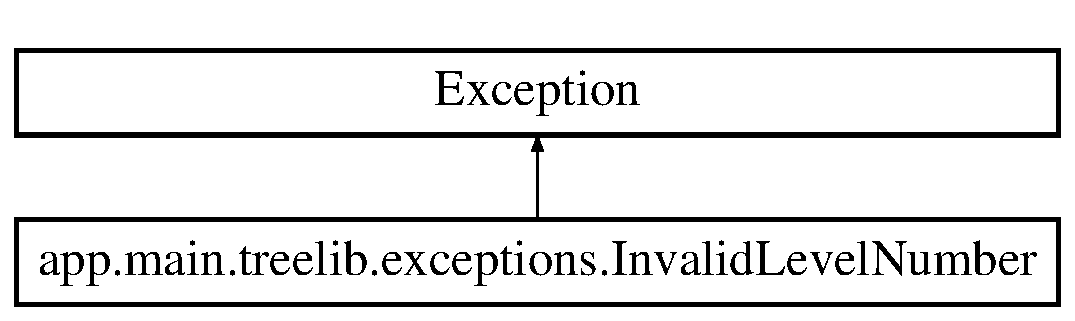
\includegraphics[height=2.000000cm]{classapp_1_1main_1_1treelib_1_1exceptions_1_1InvalidLevelNumber}
\end{center}
\end{figure}


The documentation for this class was generated from the following file\+:\begin{DoxyCompactItemize}
\item 
/home/nlarsson/bbk/python/webdev/museumflask/app/main/treelib/exceptions.\+py\end{DoxyCompactItemize}

\hypertarget{classapp_1_1main_1_1treelib_1_1exceptions_1_1LinkPastRootNodeError}{}\section{app.\+main.\+treelib.\+exceptions.\+Link\+Past\+Root\+Node\+Error Class Reference}
\label{classapp_1_1main_1_1treelib_1_1exceptions_1_1LinkPastRootNodeError}\index{app.\+main.\+treelib.\+exceptions.\+Link\+Past\+Root\+Node\+Error@{app.\+main.\+treelib.\+exceptions.\+Link\+Past\+Root\+Node\+Error}}
Inheritance diagram for app.\+main.\+treelib.\+exceptions.\+Link\+Past\+Root\+Node\+Error\+:\begin{figure}[H]
\begin{center}
\leavevmode
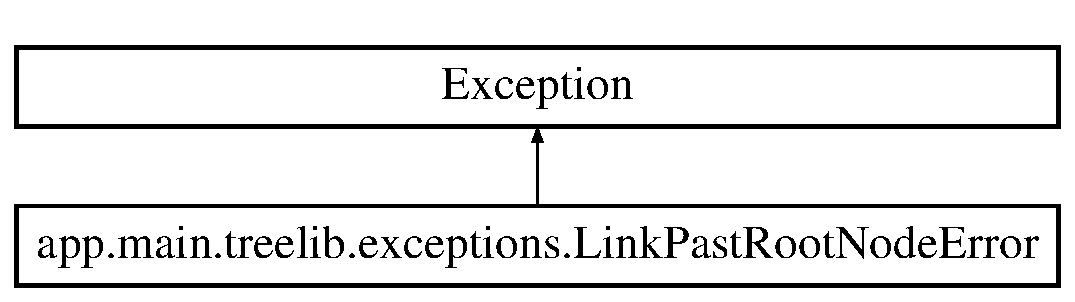
\includegraphics[height=2.000000cm]{classapp_1_1main_1_1treelib_1_1exceptions_1_1LinkPastRootNodeError}
\end{center}
\end{figure}


\subsection{Detailed Description}
\begin{DoxyVerb}Exception throwed in Tree.link_past_node() if one attempts
to "link past" the root node of a tree.
\end{DoxyVerb}
 

The documentation for this class was generated from the following file\+:\begin{DoxyCompactItemize}
\item 
/home/nlarsson/bbk/python/webdev/museumflask/app/main/treelib/exceptions.\+py\end{DoxyCompactItemize}

\hypertarget{classapp_1_1main_1_1treelib_1_1exceptions_1_1LoopError}{}\section{app.\+main.\+treelib.\+exceptions.\+Loop\+Error Class Reference}
\label{classapp_1_1main_1_1treelib_1_1exceptions_1_1LoopError}\index{app.\+main.\+treelib.\+exceptions.\+Loop\+Error@{app.\+main.\+treelib.\+exceptions.\+Loop\+Error}}
Inheritance diagram for app.\+main.\+treelib.\+exceptions.\+Loop\+Error\+:\begin{figure}[H]
\begin{center}
\leavevmode
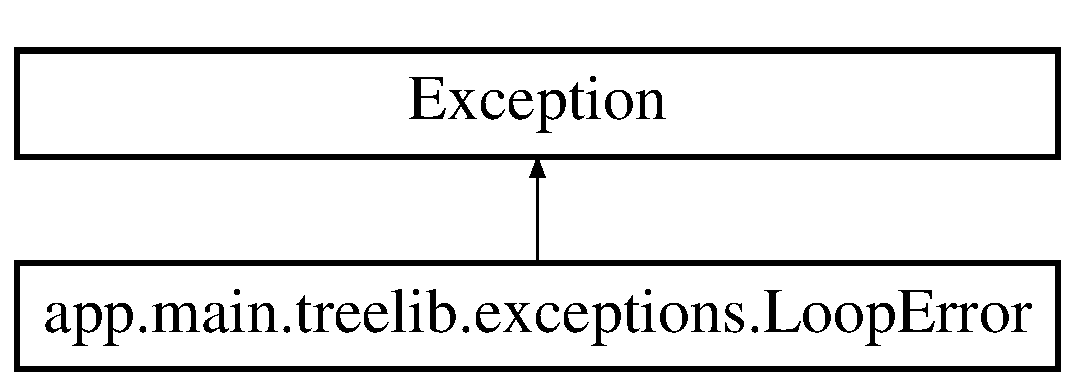
\includegraphics[height=2.000000cm]{classapp_1_1main_1_1treelib_1_1exceptions_1_1LoopError}
\end{center}
\end{figure}


\subsection{Detailed Description}
\begin{DoxyVerb}Exception thrown if trying to move node B to node A's position
while A is B's ancestor.
\end{DoxyVerb}
 

The documentation for this class was generated from the following file\+:\begin{DoxyCompactItemize}
\item 
/home/nlarsson/bbk/python/webdev/museumflask/app/main/treelib/exceptions.\+py\end{DoxyCompactItemize}

\hypertarget{classapp_1_1main_1_1mapchart_1_1MapChart}{}\section{app.\+main.\+mapchart.\+Map\+Chart Class Reference}
\label{classapp_1_1main_1_1mapchart_1_1MapChart}\index{app.\+main.\+mapchart.\+Map\+Chart@{app.\+main.\+mapchart.\+Map\+Chart}}
\subsection*{Static Public Attributes}
\begin{DoxyCompactItemize}
\item 
\mbox{\Hypertarget{classapp_1_1main_1_1mapchart_1_1MapChart_afad3f1dbe0ede0abbae15e8bed0f8e97}\label{classapp_1_1main_1_1mapchart_1_1MapChart_afad3f1dbe0ede0abbae15e8bed0f8e97}} 
{\bfseries t} = None
\item 
\mbox{\Hypertarget{classapp_1_1main_1_1mapchart_1_1MapChart_a89ef2d04ae65bd5b424193083cf91a39}\label{classapp_1_1main_1_1mapchart_1_1MapChart_a89ef2d04ae65bd5b424193083cf91a39}} 
dictionary {\bfseries boundaries} = \{\}
\item 
\mbox{\Hypertarget{classapp_1_1main_1_1mapchart_1_1MapChart_a6deb398c2b5ffa7a3b42fcd8bffaa7dc}\label{classapp_1_1main_1_1mapchart_1_1MapChart_a6deb398c2b5ffa7a3b42fcd8bffaa7dc}} 
list {\bfseries locations} = \mbox{[}\textquotesingle{}Country\textquotesingle{},\textquotesingle{}Region\textquotesingle{},\textquotesingle{}County\textquotesingle{},\textquotesingle{}Comb auth\textquotesingle{},\textquotesingle{}Local auth\textquotesingle{}\mbox{]}
\item 
\mbox{\Hypertarget{classapp_1_1main_1_1mapchart_1_1MapChart_aa53fca5d2afa66ba9b913ac99b3367d5}\label{classapp_1_1main_1_1mapchart_1_1MapChart_aa53fca5d2afa66ba9b913ac99b3367d5}} 
list {\bfseries countries} = \mbox{[}\textquotesingle{}England\textquotesingle{},\textquotesingle{}Scotland\textquotesingle{},\textquotesingle{}Northern Ireland\textquotesingle{},\textquotesingle{}Wales\textquotesingle{}\mbox{]}
\item 
\mbox{\Hypertarget{classapp_1_1main_1_1mapchart_1_1MapChart_af9ddec8e377508dac866c8973415656c}\label{classapp_1_1main_1_1mapchart_1_1MapChart_af9ddec8e377508dac866c8973415656c}} 
list {\bfseries time\+\_\+range} = \mbox{[}definitions.\+Y\+E\+A\+R\+\_\+\+O\+P\+E\+N\+ED,definitions.\+Y\+E\+A\+R\+\_\+\+C\+L\+O\+S\+ED\mbox{]}
\item 
\mbox{\Hypertarget{classapp_1_1main_1_1mapchart_1_1MapChart_acc7b67699c5df8ab1ee7995d116fd372}\label{classapp_1_1main_1_1mapchart_1_1MapChart_acc7b67699c5df8ab1ee7995d116fd372}} 
{\bfseries modeltoview} = \mbox{\hyperlink{classapp_1_1main_1_1model__to__view_1_1Model__To__View}{model\+\_\+to\+\_\+view.\+Model\+\_\+\+To\+\_\+\+View}}()
\end{DoxyCompactItemize}


The documentation for this class was generated from the following file\+:\begin{DoxyCompactItemize}
\item 
/home/nlarsson/bbk/python/webdev/museumflask/app/main/\mbox{\hyperlink{mapchart_8py}{mapchart.\+py}}\end{DoxyCompactItemize}

\hypertarget{classapp_1_1main_1_1model__to__view_1_1Model__To__View}{}\section{app.\+main.\+model\+\_\+to\+\_\+view.\+Model\+\_\+\+To\+\_\+\+View Class Reference}
\label{classapp_1_1main_1_1model__to__view_1_1Model__To__View}\index{app.\+main.\+model\+\_\+to\+\_\+view.\+Model\+\_\+\+To\+\_\+\+View@{app.\+main.\+model\+\_\+to\+\_\+view.\+Model\+\_\+\+To\+\_\+\+View}}


Purpose\+:Formats a model representation to a view representation of all datatypes.  


Inheritance diagram for app.\+main.\+model\+\_\+to\+\_\+view.\+Model\+\_\+\+To\+\_\+\+View\+:\begin{figure}[H]
\begin{center}
\leavevmode
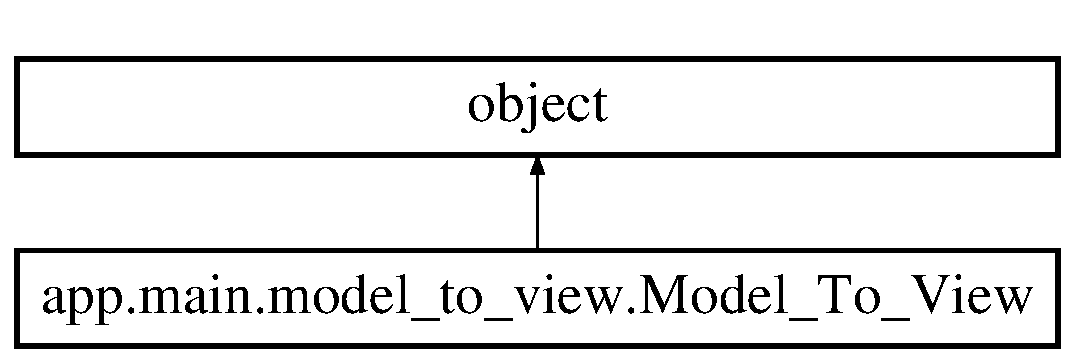
\includegraphics[height=2.000000cm]{classapp_1_1main_1_1model__to__view_1_1Model__To__View}
\end{center}
\end{figure}
\subsection*{Public Member Functions}
\begin{DoxyCompactItemize}
\item 
\mbox{\Hypertarget{classapp_1_1main_1_1model__to__view_1_1Model__To__View_ac63b92ae6be77e991cf490f0683cfd9f}\label{classapp_1_1main_1_1model__to__view_1_1Model__To__View_ac63b92ae6be77e991cf490f0683cfd9f}} 
def {\bfseries get\+View} (self, model, attribute)
\end{DoxyCompactItemize}
\subsection*{Static Public Attributes}
\begin{DoxyCompactItemize}
\item 
\mbox{\Hypertarget{classapp_1_1main_1_1model__to__view_1_1Model__To__View_ad0073ad307c0e193e93933a86bdedde2}\label{classapp_1_1main_1_1model__to__view_1_1Model__To__View_ad0073ad307c0e193e93933a86bdedde2}} 
{\bfseries parts} = attribute.\+split(definitions.\+H\+I\+E\+R\+\_\+\+S\+E\+P\+A\+R\+A\+T\+OR)
\item 
\mbox{\Hypertarget{classapp_1_1main_1_1model__to__view_1_1Model__To__View_a21ce3063ed1c03e10bd09dc2d3018d20}\label{classapp_1_1main_1_1model__to__view_1_1Model__To__View_a21ce3063ed1c03e10bd09dc2d3018d20}} 
{\bfseries lastpart} = parts\mbox{[}len(parts)-\/1\mbox{]}
\item 
\mbox{\Hypertarget{classapp_1_1main_1_1model__to__view_1_1Model__To__View_a94de482d624c64f0d992a51ba7e1ebe2}\label{classapp_1_1main_1_1model__to__view_1_1Model__To__View_a94de482d624c64f0d992a51ba7e1ebe2}} 
{\bfseries vals} = attribute.\+split(definitions.\+R\+A\+N\+G\+E\+\_\+\+S\+E\+P\+A\+R\+A\+T\+OR)
\item 
\mbox{\Hypertarget{classapp_1_1main_1_1model__to__view_1_1Model__To__View_a6df97d85268e379273f38e3e505c0fca}\label{classapp_1_1main_1_1model__to__view_1_1Model__To__View_a6df97d85268e379273f38e3e505c0fca}} 
{\bfseries instance} = apputils.\+get\+Data\+Class\+Instance(definitions.\+S\+T\+A\+T\+U\+S\+C\+H\+A\+N\+GE)
\item 
\mbox{\Hypertarget{classapp_1_1main_1_1model__to__view_1_1Model__To__View_a0eecdb417dbdfd70e65bde6a5cf3dfda}\label{classapp_1_1main_1_1model__to__view_1_1Model__To__View_a0eecdb417dbdfd70e65bde6a5cf3dfda}} 
{\bfseries view} = instance.\+get\+Model\+To\+View(attribute)
\end{DoxyCompactItemize}


\subsection{Detailed Description}
Purpose\+:Formats a model representation to a view representation of all datatypes. 

Arguments\+:

The datatype of the attribute  The model representation 

The documentation for this class was generated from the following file\+:\begin{DoxyCompactItemize}
\item 
/home/nlarsson/bbk/python/webdev/museumflask/app/main/\mbox{\hyperlink{model__to__view_8py}{model\+\_\+to\+\_\+view.\+py}}\end{DoxyCompactItemize}

\hypertarget{classapp_1_1main_1_1treelib_1_1exceptions_1_1MultipleRootError}{}\section{app.\+main.\+treelib.\+exceptions.\+Multiple\+Root\+Error Class Reference}
\label{classapp_1_1main_1_1treelib_1_1exceptions_1_1MultipleRootError}\index{app.\+main.\+treelib.\+exceptions.\+Multiple\+Root\+Error@{app.\+main.\+treelib.\+exceptions.\+Multiple\+Root\+Error}}
Inheritance diagram for app.\+main.\+treelib.\+exceptions.\+Multiple\+Root\+Error\+:\begin{figure}[H]
\begin{center}
\leavevmode
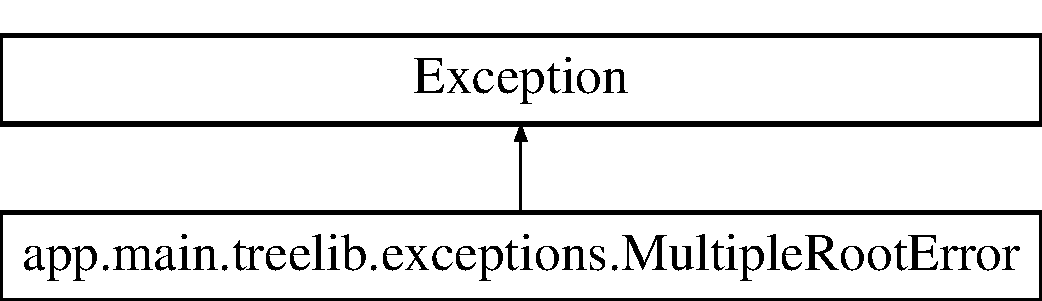
\includegraphics[height=2.000000cm]{classapp_1_1main_1_1treelib_1_1exceptions_1_1MultipleRootError}
\end{center}
\end{figure}


\subsection{Detailed Description}
\begin{DoxyVerb}Exception throwed if more than one root exists in a tree.\end{DoxyVerb}
 

The documentation for this class was generated from the following file\+:\begin{DoxyCompactItemize}
\item 
/home/nlarsson/bbk/python/webdev/museumflask/app/main/treelib/exceptions.\+py\end{DoxyCompactItemize}

\hypertarget{classapp_1_1main_1_1nakedid_1_1NakedId}{}\section{app.\+main.\+nakedid.\+Naked\+Id Class Reference}
\label{classapp_1_1main_1_1nakedid_1_1NakedId}\index{app.\+main.\+nakedid.\+Naked\+Id@{app.\+main.\+nakedid.\+Naked\+Id}}
\subsection*{Static Public Attributes}
\begin{DoxyCompactItemize}
\item 
\mbox{\Hypertarget{classapp_1_1main_1_1nakedid_1_1NakedId_aa100f474e0b55cfd8e2269bc74879fa2}\label{classapp_1_1main_1_1nakedid_1_1NakedId_aa100f474e0b55cfd8e2269bc74879fa2}} 
{\bfseries modeltoview} = \mbox{\hyperlink{classapp_1_1main_1_1model__to__view_1_1Model__To__View}{model\+\_\+to\+\_\+view.\+Model\+\_\+\+To\+\_\+\+View}}()
\end{DoxyCompactItemize}


The documentation for this class was generated from the following file\+:\begin{DoxyCompactItemize}
\item 
/home/nlarsson/bbk/python/webdev/museumflask/app/main/\mbox{\hyperlink{nakedid_8py}{nakedid.\+py}}\end{DoxyCompactItemize}

\hypertarget{classapp_1_1main_1_1treelib_1_1node_1_1Node}{}\section{app.\+main.\+treelib.\+node.\+Node Class Reference}
\label{classapp_1_1main_1_1treelib_1_1node_1_1Node}\index{app.\+main.\+treelib.\+node.\+Node@{app.\+main.\+treelib.\+node.\+Node}}
Inheritance diagram for app.\+main.\+treelib.\+node.\+Node\+:\begin{figure}[H]
\begin{center}
\leavevmode
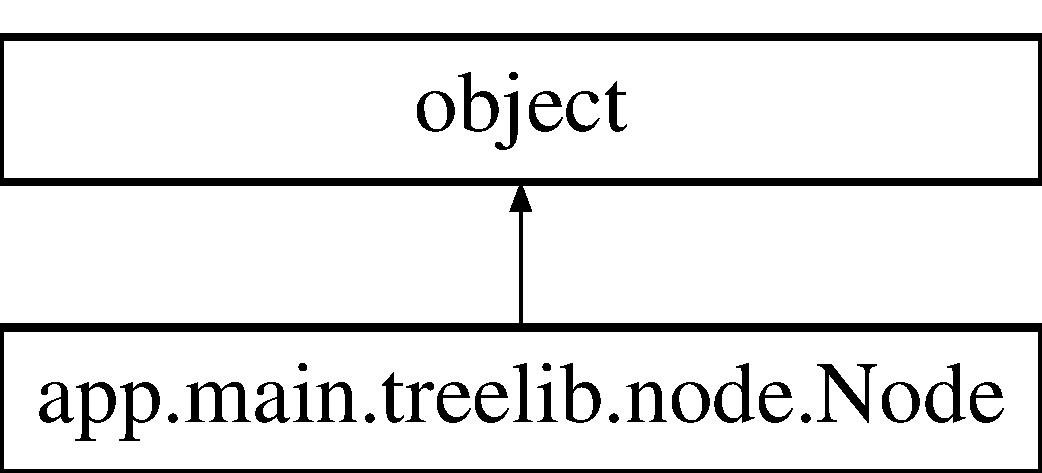
\includegraphics[height=2.000000cm]{classapp_1_1main_1_1treelib_1_1node_1_1Node}
\end{center}
\end{figure}
\subsection*{Public Member Functions}
\begin{DoxyCompactItemize}
\item 
def \mbox{\hyperlink{classapp_1_1main_1_1treelib_1_1node_1_1Node_aac2165277078b78954b973a74fd68ba6}{\+\_\+\+\_\+init\+\_\+\+\_\+}} (self, \mbox{\hyperlink{classapp_1_1main_1_1treelib_1_1node_1_1Node_a5ddde76bda1e158e64eab1dc17712af6}{tag}}=None, \mbox{\hyperlink{classapp_1_1main_1_1treelib_1_1node_1_1Node_a8ef90e787789eb8af60606d46255564f}{identifier}}=None, expanded=True, data=None)
\item 
\mbox{\Hypertarget{classapp_1_1main_1_1treelib_1_1node_1_1Node_a8e57640cfd3cceaf2a435810b907c096}\label{classapp_1_1main_1_1treelib_1_1node_1_1Node_a8e57640cfd3cceaf2a435810b907c096}} 
def {\bfseries \+\_\+\+\_\+lt\+\_\+\+\_\+} (self, other)
\item 
def \mbox{\hyperlink{classapp_1_1main_1_1treelib_1_1node_1_1Node_a55bc875d07efd5ef95890c57882d3578}{bpointer}} (self)
\item 
def \mbox{\hyperlink{classapp_1_1main_1_1treelib_1_1node_1_1Node_a74a05c3d863c43f25536f44b5e392932}{bpointer}} (self, nid)
\item 
def \mbox{\hyperlink{classapp_1_1main_1_1treelib_1_1node_1_1Node_a98442ca873604524b806978aca72addb}{fpointer}} (self)
\item 
def \mbox{\hyperlink{classapp_1_1main_1_1treelib_1_1node_1_1Node_afc312003b4159b00d8ed55fed0680474}{fpointer}} (self, value)
\item 
def \mbox{\hyperlink{classapp_1_1main_1_1treelib_1_1node_1_1Node_a8ef90e787789eb8af60606d46255564f}{identifier}} (self)
\item 
def \mbox{\hyperlink{classapp_1_1main_1_1treelib_1_1node_1_1Node_af0558bf5b5af7eb1b3b2ced14c50e869}{identifier}} (self, value)
\item 
def \mbox{\hyperlink{classapp_1_1main_1_1treelib_1_1node_1_1Node_ada4b689dcebea9b5b1adc7949b40e3d0}{is\+\_\+leaf}} (self)
\item 
def \mbox{\hyperlink{classapp_1_1main_1_1treelib_1_1node_1_1Node_a3e70bbc4a3f2e1642546769b4bc82949}{is\+\_\+root}} (self)
\item 
def \mbox{\hyperlink{classapp_1_1main_1_1treelib_1_1node_1_1Node_a5ddde76bda1e158e64eab1dc17712af6}{tag}} (self)
\item 
def \mbox{\hyperlink{classapp_1_1main_1_1treelib_1_1node_1_1Node_adce76642226ce58f591191ba3314797c}{tag}} (self, value)
\item 
def \mbox{\hyperlink{classapp_1_1main_1_1treelib_1_1node_1_1Node_ad5123f1013b32f2d3fc3c6aa82897a8f}{update\+\_\+bpointer}} (self, nid)
\item 
def \mbox{\hyperlink{classapp_1_1main_1_1treelib_1_1node_1_1Node_a1c2773beab05416bc58d9e5063b58590}{update\+\_\+fpointer}} (self, nid, mode=A\+DD, replace=None)
\item 
\mbox{\Hypertarget{classapp_1_1main_1_1treelib_1_1node_1_1Node_a208ec50bee77d4ff1d920ecd6cfbf0d1}\label{classapp_1_1main_1_1treelib_1_1node_1_1Node_a208ec50bee77d4ff1d920ecd6cfbf0d1}} 
def {\bfseries \+\_\+\+\_\+repr\+\_\+\+\_\+} (self)
\end{DoxyCompactItemize}
\subsection*{Public Attributes}
\begin{DoxyCompactItemize}
\item 
\mbox{\Hypertarget{classapp_1_1main_1_1treelib_1_1node_1_1Node_a6a5c835203738fa4fd7f5fdd7358ebbd}\label{classapp_1_1main_1_1treelib_1_1node_1_1Node_a6a5c835203738fa4fd7f5fdd7358ebbd}} 
{\bfseries expanded}
\item 
\mbox{\Hypertarget{classapp_1_1main_1_1treelib_1_1node_1_1Node_aec761d3090512fa2151eccd678a36e1a}\label{classapp_1_1main_1_1treelib_1_1node_1_1Node_aec761d3090512fa2151eccd678a36e1a}} 
{\bfseries data}
\item 
\mbox{\Hypertarget{classapp_1_1main_1_1treelib_1_1node_1_1Node_abba86dbedcc40b7635bdb1fcee1e7f08}\label{classapp_1_1main_1_1treelib_1_1node_1_1Node_abba86dbedcc40b7635bdb1fcee1e7f08}} 
{\bfseries bpointer}
\end{DoxyCompactItemize}


\subsection{Detailed Description}
\begin{DoxyVerb}Nodes are elementary objects which are stored a `_nodes` dictionary of a Tree.
Use `data` attribute to store node-specific data.
\end{DoxyVerb}
 

\subsection{Constructor \& Destructor Documentation}
\mbox{\Hypertarget{classapp_1_1main_1_1treelib_1_1node_1_1Node_aac2165277078b78954b973a74fd68ba6}\label{classapp_1_1main_1_1treelib_1_1node_1_1Node_aac2165277078b78954b973a74fd68ba6}} 
\index{app\+::main\+::treelib\+::node\+::\+Node@{app\+::main\+::treelib\+::node\+::\+Node}!\+\_\+\+\_\+init\+\_\+\+\_\+@{\+\_\+\+\_\+init\+\_\+\+\_\+}}
\index{\+\_\+\+\_\+init\+\_\+\+\_\+@{\+\_\+\+\_\+init\+\_\+\+\_\+}!app\+::main\+::treelib\+::node\+::\+Node@{app\+::main\+::treelib\+::node\+::\+Node}}
\subsubsection{\texorpdfstring{\+\_\+\+\_\+init\+\_\+\+\_\+()}{\_\_init\_\_()}}
{\footnotesize\ttfamily def app.\+main.\+treelib.\+node.\+Node.\+\_\+\+\_\+init\+\_\+\+\_\+ (\begin{DoxyParamCaption}\item[{}]{self,  }\item[{}]{tag = {\ttfamily None},  }\item[{}]{identifier = {\ttfamily None},  }\item[{}]{expanded = {\ttfamily True},  }\item[{}]{data = {\ttfamily None} }\end{DoxyParamCaption})}

\begin{DoxyVerb}Create a new Node object to be placed inside a Tree object\end{DoxyVerb}
 

\subsection{Member Function Documentation}
\mbox{\Hypertarget{classapp_1_1main_1_1treelib_1_1node_1_1Node_a55bc875d07efd5ef95890c57882d3578}\label{classapp_1_1main_1_1treelib_1_1node_1_1Node_a55bc875d07efd5ef95890c57882d3578}} 
\index{app\+::main\+::treelib\+::node\+::\+Node@{app\+::main\+::treelib\+::node\+::\+Node}!bpointer@{bpointer}}
\index{bpointer@{bpointer}!app\+::main\+::treelib\+::node\+::\+Node@{app\+::main\+::treelib\+::node\+::\+Node}}
\subsubsection{\texorpdfstring{bpointer()}{bpointer()}\hspace{0.1cm}{\footnotesize\ttfamily [1/2]}}
{\footnotesize\ttfamily def app.\+main.\+treelib.\+node.\+Node.\+bpointer (\begin{DoxyParamCaption}\item[{}]{self }\end{DoxyParamCaption})}

\begin{DoxyVerb}Return the value of `_bpointer`.\end{DoxyVerb}
 \mbox{\Hypertarget{classapp_1_1main_1_1treelib_1_1node_1_1Node_a74a05c3d863c43f25536f44b5e392932}\label{classapp_1_1main_1_1treelib_1_1node_1_1Node_a74a05c3d863c43f25536f44b5e392932}} 
\index{app\+::main\+::treelib\+::node\+::\+Node@{app\+::main\+::treelib\+::node\+::\+Node}!bpointer@{bpointer}}
\index{bpointer@{bpointer}!app\+::main\+::treelib\+::node\+::\+Node@{app\+::main\+::treelib\+::node\+::\+Node}}
\subsubsection{\texorpdfstring{bpointer()}{bpointer()}\hspace{0.1cm}{\footnotesize\ttfamily [2/2]}}
{\footnotesize\ttfamily def app.\+main.\+treelib.\+node.\+Node.\+bpointer (\begin{DoxyParamCaption}\item[{}]{self,  }\item[{}]{nid }\end{DoxyParamCaption})}

\begin{DoxyVerb}Set the value of `_bpointer`.\end{DoxyVerb}
 \mbox{\Hypertarget{classapp_1_1main_1_1treelib_1_1node_1_1Node_a98442ca873604524b806978aca72addb}\label{classapp_1_1main_1_1treelib_1_1node_1_1Node_a98442ca873604524b806978aca72addb}} 
\index{app\+::main\+::treelib\+::node\+::\+Node@{app\+::main\+::treelib\+::node\+::\+Node}!fpointer@{fpointer}}
\index{fpointer@{fpointer}!app\+::main\+::treelib\+::node\+::\+Node@{app\+::main\+::treelib\+::node\+::\+Node}}
\subsubsection{\texorpdfstring{fpointer()}{fpointer()}\hspace{0.1cm}{\footnotesize\ttfamily [1/2]}}
{\footnotesize\ttfamily def app.\+main.\+treelib.\+node.\+Node.\+fpointer (\begin{DoxyParamCaption}\item[{}]{self }\end{DoxyParamCaption})}

\begin{DoxyVerb}Return the value of `_fpointer`.\end{DoxyVerb}
 \mbox{\Hypertarget{classapp_1_1main_1_1treelib_1_1node_1_1Node_afc312003b4159b00d8ed55fed0680474}\label{classapp_1_1main_1_1treelib_1_1node_1_1Node_afc312003b4159b00d8ed55fed0680474}} 
\index{app\+::main\+::treelib\+::node\+::\+Node@{app\+::main\+::treelib\+::node\+::\+Node}!fpointer@{fpointer}}
\index{fpointer@{fpointer}!app\+::main\+::treelib\+::node\+::\+Node@{app\+::main\+::treelib\+::node\+::\+Node}}
\subsubsection{\texorpdfstring{fpointer()}{fpointer()}\hspace{0.1cm}{\footnotesize\ttfamily [2/2]}}
{\footnotesize\ttfamily def app.\+main.\+treelib.\+node.\+Node.\+fpointer (\begin{DoxyParamCaption}\item[{}]{self,  }\item[{}]{value }\end{DoxyParamCaption})}

\begin{DoxyVerb}Set the value of `_fpointer`.\end{DoxyVerb}
 \mbox{\Hypertarget{classapp_1_1main_1_1treelib_1_1node_1_1Node_a8ef90e787789eb8af60606d46255564f}\label{classapp_1_1main_1_1treelib_1_1node_1_1Node_a8ef90e787789eb8af60606d46255564f}} 
\index{app\+::main\+::treelib\+::node\+::\+Node@{app\+::main\+::treelib\+::node\+::\+Node}!identifier@{identifier}}
\index{identifier@{identifier}!app\+::main\+::treelib\+::node\+::\+Node@{app\+::main\+::treelib\+::node\+::\+Node}}
\subsubsection{\texorpdfstring{identifier()}{identifier()}\hspace{0.1cm}{\footnotesize\ttfamily [1/2]}}
{\footnotesize\ttfamily def app.\+main.\+treelib.\+node.\+Node.\+identifier (\begin{DoxyParamCaption}\item[{}]{self }\end{DoxyParamCaption})}

\begin{DoxyVerb}Return the value of `_identifier`.\end{DoxyVerb}
 \mbox{\Hypertarget{classapp_1_1main_1_1treelib_1_1node_1_1Node_af0558bf5b5af7eb1b3b2ced14c50e869}\label{classapp_1_1main_1_1treelib_1_1node_1_1Node_af0558bf5b5af7eb1b3b2ced14c50e869}} 
\index{app\+::main\+::treelib\+::node\+::\+Node@{app\+::main\+::treelib\+::node\+::\+Node}!identifier@{identifier}}
\index{identifier@{identifier}!app\+::main\+::treelib\+::node\+::\+Node@{app\+::main\+::treelib\+::node\+::\+Node}}
\subsubsection{\texorpdfstring{identifier()}{identifier()}\hspace{0.1cm}{\footnotesize\ttfamily [2/2]}}
{\footnotesize\ttfamily def app.\+main.\+treelib.\+node.\+Node.\+identifier (\begin{DoxyParamCaption}\item[{}]{self,  }\item[{}]{value }\end{DoxyParamCaption})}

\begin{DoxyVerb}Set the value of `_identifier`.\end{DoxyVerb}
 \mbox{\Hypertarget{classapp_1_1main_1_1treelib_1_1node_1_1Node_ada4b689dcebea9b5b1adc7949b40e3d0}\label{classapp_1_1main_1_1treelib_1_1node_1_1Node_ada4b689dcebea9b5b1adc7949b40e3d0}} 
\index{app\+::main\+::treelib\+::node\+::\+Node@{app\+::main\+::treelib\+::node\+::\+Node}!is\+\_\+leaf@{is\+\_\+leaf}}
\index{is\+\_\+leaf@{is\+\_\+leaf}!app\+::main\+::treelib\+::node\+::\+Node@{app\+::main\+::treelib\+::node\+::\+Node}}
\subsubsection{\texorpdfstring{is\+\_\+leaf()}{is\_leaf()}}
{\footnotesize\ttfamily def app.\+main.\+treelib.\+node.\+Node.\+is\+\_\+leaf (\begin{DoxyParamCaption}\item[{}]{self }\end{DoxyParamCaption})}

\begin{DoxyVerb}Return true if current node has no children.\end{DoxyVerb}
 \mbox{\Hypertarget{classapp_1_1main_1_1treelib_1_1node_1_1Node_a3e70bbc4a3f2e1642546769b4bc82949}\label{classapp_1_1main_1_1treelib_1_1node_1_1Node_a3e70bbc4a3f2e1642546769b4bc82949}} 
\index{app\+::main\+::treelib\+::node\+::\+Node@{app\+::main\+::treelib\+::node\+::\+Node}!is\+\_\+root@{is\+\_\+root}}
\index{is\+\_\+root@{is\+\_\+root}!app\+::main\+::treelib\+::node\+::\+Node@{app\+::main\+::treelib\+::node\+::\+Node}}
\subsubsection{\texorpdfstring{is\+\_\+root()}{is\_root()}}
{\footnotesize\ttfamily def app.\+main.\+treelib.\+node.\+Node.\+is\+\_\+root (\begin{DoxyParamCaption}\item[{}]{self }\end{DoxyParamCaption})}

\begin{DoxyVerb}Return true if self has no parent, i.e. as root.\end{DoxyVerb}
 \mbox{\Hypertarget{classapp_1_1main_1_1treelib_1_1node_1_1Node_a5ddde76bda1e158e64eab1dc17712af6}\label{classapp_1_1main_1_1treelib_1_1node_1_1Node_a5ddde76bda1e158e64eab1dc17712af6}} 
\index{app\+::main\+::treelib\+::node\+::\+Node@{app\+::main\+::treelib\+::node\+::\+Node}!tag@{tag}}
\index{tag@{tag}!app\+::main\+::treelib\+::node\+::\+Node@{app\+::main\+::treelib\+::node\+::\+Node}}
\subsubsection{\texorpdfstring{tag()}{tag()}\hspace{0.1cm}{\footnotesize\ttfamily [1/2]}}
{\footnotesize\ttfamily def app.\+main.\+treelib.\+node.\+Node.\+tag (\begin{DoxyParamCaption}\item[{}]{self }\end{DoxyParamCaption})}

\begin{DoxyVerb}Return the value of `_tag`.\end{DoxyVerb}
 \mbox{\Hypertarget{classapp_1_1main_1_1treelib_1_1node_1_1Node_adce76642226ce58f591191ba3314797c}\label{classapp_1_1main_1_1treelib_1_1node_1_1Node_adce76642226ce58f591191ba3314797c}} 
\index{app\+::main\+::treelib\+::node\+::\+Node@{app\+::main\+::treelib\+::node\+::\+Node}!tag@{tag}}
\index{tag@{tag}!app\+::main\+::treelib\+::node\+::\+Node@{app\+::main\+::treelib\+::node\+::\+Node}}
\subsubsection{\texorpdfstring{tag()}{tag()}\hspace{0.1cm}{\footnotesize\ttfamily [2/2]}}
{\footnotesize\ttfamily def app.\+main.\+treelib.\+node.\+Node.\+tag (\begin{DoxyParamCaption}\item[{}]{self,  }\item[{}]{value }\end{DoxyParamCaption})}

\begin{DoxyVerb}Set the value of `_tag`.\end{DoxyVerb}
 \mbox{\Hypertarget{classapp_1_1main_1_1treelib_1_1node_1_1Node_ad5123f1013b32f2d3fc3c6aa82897a8f}\label{classapp_1_1main_1_1treelib_1_1node_1_1Node_ad5123f1013b32f2d3fc3c6aa82897a8f}} 
\index{app\+::main\+::treelib\+::node\+::\+Node@{app\+::main\+::treelib\+::node\+::\+Node}!update\+\_\+bpointer@{update\+\_\+bpointer}}
\index{update\+\_\+bpointer@{update\+\_\+bpointer}!app\+::main\+::treelib\+::node\+::\+Node@{app\+::main\+::treelib\+::node\+::\+Node}}
\subsubsection{\texorpdfstring{update\+\_\+bpointer()}{update\_bpointer()}}
{\footnotesize\ttfamily def app.\+main.\+treelib.\+node.\+Node.\+update\+\_\+bpointer (\begin{DoxyParamCaption}\item[{}]{self,  }\item[{}]{nid }\end{DoxyParamCaption})}

\begin{DoxyVerb}Update parent node.\end{DoxyVerb}
 \mbox{\Hypertarget{classapp_1_1main_1_1treelib_1_1node_1_1Node_a1c2773beab05416bc58d9e5063b58590}\label{classapp_1_1main_1_1treelib_1_1node_1_1Node_a1c2773beab05416bc58d9e5063b58590}} 
\index{app\+::main\+::treelib\+::node\+::\+Node@{app\+::main\+::treelib\+::node\+::\+Node}!update\+\_\+fpointer@{update\+\_\+fpointer}}
\index{update\+\_\+fpointer@{update\+\_\+fpointer}!app\+::main\+::treelib\+::node\+::\+Node@{app\+::main\+::treelib\+::node\+::\+Node}}
\subsubsection{\texorpdfstring{update\+\_\+fpointer()}{update\_fpointer()}}
{\footnotesize\ttfamily def app.\+main.\+treelib.\+node.\+Node.\+update\+\_\+fpointer (\begin{DoxyParamCaption}\item[{}]{self,  }\item[{}]{nid,  }\item[{}]{mode = {\ttfamily ADD},  }\item[{}]{replace = {\ttfamily None} }\end{DoxyParamCaption})}

\begin{DoxyVerb}Update all children nodes.\end{DoxyVerb}
 

The documentation for this class was generated from the following file\+:\begin{DoxyCompactItemize}
\item 
/home/nlarsson/bbk/python/webdev/museumflask/app/main/treelib/node.\+py\end{DoxyCompactItemize}

\hypertarget{classapp_1_1main_1_1treelib_1_1exceptions_1_1NodeIDAbsentError}{}\section{app.\+main.\+treelib.\+exceptions.\+Node\+I\+D\+Absent\+Error Class Reference}
\label{classapp_1_1main_1_1treelib_1_1exceptions_1_1NodeIDAbsentError}\index{app.\+main.\+treelib.\+exceptions.\+Node\+I\+D\+Absent\+Error@{app.\+main.\+treelib.\+exceptions.\+Node\+I\+D\+Absent\+Error}}
Inheritance diagram for app.\+main.\+treelib.\+exceptions.\+Node\+I\+D\+Absent\+Error\+:\begin{figure}[H]
\begin{center}
\leavevmode
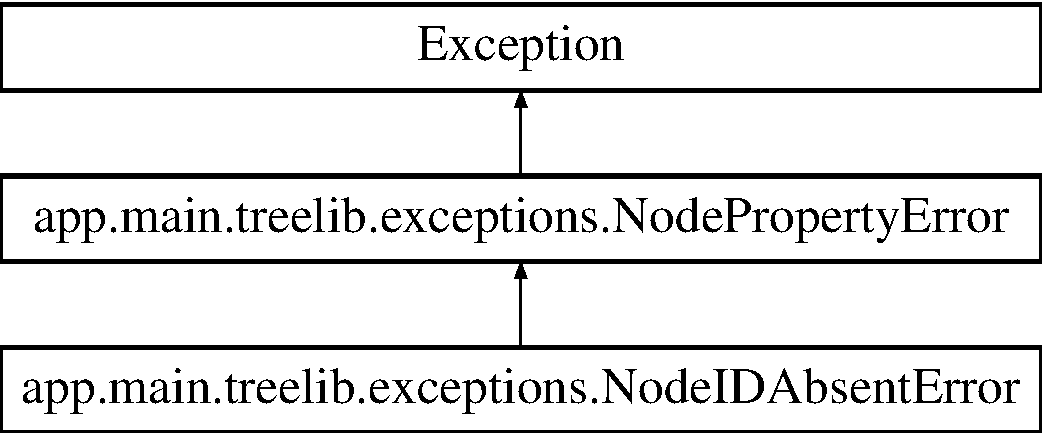
\includegraphics[height=3.000000cm]{classapp_1_1main_1_1treelib_1_1exceptions_1_1NodeIDAbsentError}
\end{center}
\end{figure}


\subsection{Detailed Description}
\begin{DoxyVerb}Exception throwed if a node's identifier is unknown\end{DoxyVerb}
 

The documentation for this class was generated from the following file\+:\begin{DoxyCompactItemize}
\item 
/home/nlarsson/bbk/python/webdev/museumflask/app/main/treelib/exceptions.\+py\end{DoxyCompactItemize}

\hypertarget{classapp_1_1main_1_1treelib_1_1exceptions_1_1NodePropertyAbsentError}{}\section{app.\+main.\+treelib.\+exceptions.\+Node\+Property\+Absent\+Error Class Reference}
\label{classapp_1_1main_1_1treelib_1_1exceptions_1_1NodePropertyAbsentError}\index{app.\+main.\+treelib.\+exceptions.\+Node\+Property\+Absent\+Error@{app.\+main.\+treelib.\+exceptions.\+Node\+Property\+Absent\+Error}}
Inheritance diagram for app.\+main.\+treelib.\+exceptions.\+Node\+Property\+Absent\+Error\+:\begin{figure}[H]
\begin{center}
\leavevmode
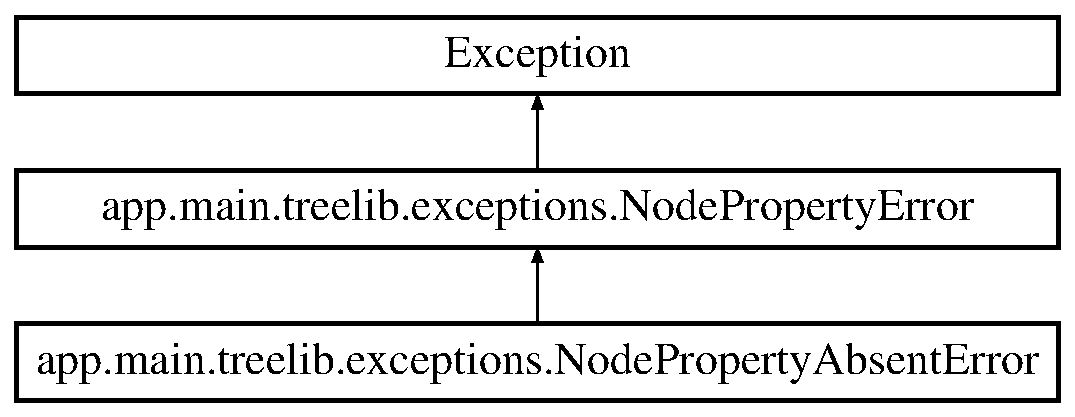
\includegraphics[height=3.000000cm]{classapp_1_1main_1_1treelib_1_1exceptions_1_1NodePropertyAbsentError}
\end{center}
\end{figure}


\subsection{Detailed Description}
\begin{DoxyVerb}Exception throwed if a node's data property is not specified\end{DoxyVerb}
 

The documentation for this class was generated from the following file\+:\begin{DoxyCompactItemize}
\item 
/home/nlarsson/bbk/python/webdev/museumflask/app/main/treelib/exceptions.\+py\end{DoxyCompactItemize}

\hypertarget{classapp_1_1main_1_1treelib_1_1exceptions_1_1NodePropertyError}{}\section{app.\+main.\+treelib.\+exceptions.\+Node\+Property\+Error Class Reference}
\label{classapp_1_1main_1_1treelib_1_1exceptions_1_1NodePropertyError}\index{app.\+main.\+treelib.\+exceptions.\+Node\+Property\+Error@{app.\+main.\+treelib.\+exceptions.\+Node\+Property\+Error}}
Inheritance diagram for app.\+main.\+treelib.\+exceptions.\+Node\+Property\+Error\+:\begin{figure}[H]
\begin{center}
\leavevmode
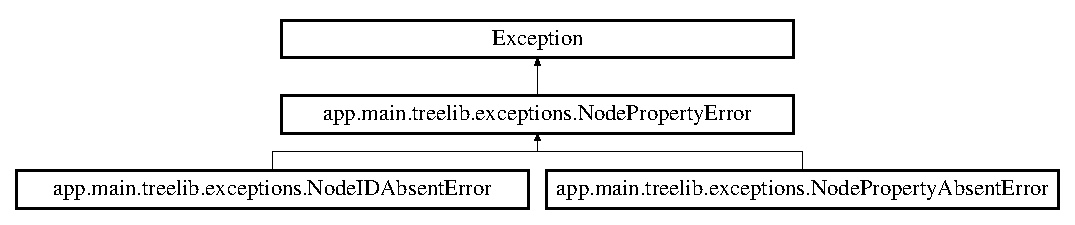
\includegraphics[height=2.576687cm]{classapp_1_1main_1_1treelib_1_1exceptions_1_1NodePropertyError}
\end{center}
\end{figure}


\subsection{Detailed Description}
\begin{DoxyVerb}Basic Node attribute error\end{DoxyVerb}
 

The documentation for this class was generated from the following file\+:\begin{DoxyCompactItemize}
\item 
/home/nlarsson/bbk/python/webdev/museumflask/app/main/treelib/exceptions.\+py\end{DoxyCompactItemize}

\hypertarget{classapp_1_1main_1_1boks_1_1Boks_1_1open__at__a__given__time}{}\section{app.\+main.\+boks.\+Boks.\+open\+\_\+at\+\_\+a\+\_\+given\+\_\+time Class Reference}
\label{classapp_1_1main_1_1boks_1_1Boks_1_1open__at__a__given__time}\index{app.\+main.\+boks.\+Boks.\+open\+\_\+at\+\_\+a\+\_\+given\+\_\+time@{app.\+main.\+boks.\+Boks.\+open\+\_\+at\+\_\+a\+\_\+given\+\_\+time}}
\subsection*{Public Member Functions}
\begin{DoxyCompactItemize}
\item 
\mbox{\Hypertarget{classapp_1_1main_1_1boks_1_1Boks_1_1open__at__a__given__time_afdaf1cbfff07ebbeb6f1478a872d9f93}\label{classapp_1_1main_1_1boks_1_1Boks_1_1open__at__a__given__time_afdaf1cbfff07ebbeb6f1478a872d9f93}} 
def {\bfseries Governance} (self, me, parameters=None, contextdict=None)
\item 
\mbox{\Hypertarget{classapp_1_1main_1_1boks_1_1Boks_1_1open__at__a__given__time_a5d4218594c77f274211ab47ab0750740}\label{classapp_1_1main_1_1boks_1_1Boks_1_1open__at__a__given__time_a5d4218594c77f274211ab47ab0750740}} 
def {\bfseries Subject\+\_\+\+Matter} (self, me, parameters=None, contextdict=None)
\item 
\mbox{\Hypertarget{classapp_1_1main_1_1boks_1_1Boks_1_1open__at__a__given__time_af23eb0b7485fbfdec6711e2b693fb6c3}\label{classapp_1_1main_1_1boks_1_1Boks_1_1open__at__a__given__time_af23eb0b7485fbfdec6711e2b693fb6c3}} 
def {\bfseries Size} (self, me, parameters=None, contextdict=None)
\item 
\mbox{\Hypertarget{classapp_1_1main_1_1boks_1_1Boks_1_1open__at__a__given__time_ad37d4deb536414839684ee82681805ae}\label{classapp_1_1main_1_1boks_1_1Boks_1_1open__at__a__given__time_ad37d4deb536414839684ee82681805ae}} 
def {\bfseries All} (self, me, parameters=None, contextdict=None)
\item 
\mbox{\Hypertarget{classapp_1_1main_1_1boks_1_1Boks_1_1open__at__a__given__time_a83ee856d6b8ba8e26481b1476e2d1851}\label{classapp_1_1main_1_1boks_1_1Boks_1_1open__at__a__given__time_a83ee856d6b8ba8e26481b1476e2d1851}} 
def {\bfseries Location} (self, me, parameters=None, contextdict=None)
\end{DoxyCompactItemize}
\subsection*{Static Public Attributes}
\begin{DoxyCompactItemize}
\item 
\mbox{\Hypertarget{classapp_1_1main_1_1boks_1_1Boks_1_1open__at__a__given__time_a85c47931f8dbf803becac0a56a760dbc}\label{classapp_1_1main_1_1boks_1_1Boks_1_1open__at__a__given__time_a85c47931f8dbf803becac0a56a760dbc}} 
{\bfseries plot} = Boks.\+categorybar.\+create\+Plot(me,newparameters,contextdict)
\end{DoxyCompactItemize}


The documentation for this class was generated from the following file\+:\begin{DoxyCompactItemize}
\item 
/home/nlarsson/bbk/python/webdev/museumflask/app/main/\mbox{\hyperlink{boks_8py}{boks.\+py}}\end{DoxyCompactItemize}

\hypertarget{classapp_1_1main_1_1boks_1_1Boks_1_1open__over__time}{}\section{app.\+main.\+boks.\+Boks.\+open\+\_\+over\+\_\+time Class Reference}
\label{classapp_1_1main_1_1boks_1_1Boks_1_1open__over__time}\index{app.\+main.\+boks.\+Boks.\+open\+\_\+over\+\_\+time@{app.\+main.\+boks.\+Boks.\+open\+\_\+over\+\_\+time}}
\subsection*{Public Member Functions}
\begin{DoxyCompactItemize}
\item 
\mbox{\Hypertarget{classapp_1_1main_1_1boks_1_1Boks_1_1open__over__time_a9728d9fedb2b3f37680fbc43f8e224b2}\label{classapp_1_1main_1_1boks_1_1Boks_1_1open__over__time_a9728d9fedb2b3f37680fbc43f8e224b2}} 
def {\bfseries Governance} (self, me, parameters=None, contextdict=None)
\item 
\mbox{\Hypertarget{classapp_1_1main_1_1boks_1_1Boks_1_1open__over__time_acb911674c3b70842f7df84f3e1789095}\label{classapp_1_1main_1_1boks_1_1Boks_1_1open__over__time_acb911674c3b70842f7df84f3e1789095}} 
def {\bfseries Subject\+\_\+\+Matter} (self, me, parameters=None, contextdict=None)
\item 
\mbox{\Hypertarget{classapp_1_1main_1_1boks_1_1Boks_1_1open__over__time_a02570582a07a69d7725030c52e8cc8ca}\label{classapp_1_1main_1_1boks_1_1Boks_1_1open__over__time_a02570582a07a69d7725030c52e8cc8ca}} 
def {\bfseries Size} (self, me, parameters=None, contextdict=None)
\item 
\mbox{\Hypertarget{classapp_1_1main_1_1boks_1_1Boks_1_1open__over__time_a39f54a906b1ec3807310c4daf56c9369}\label{classapp_1_1main_1_1boks_1_1Boks_1_1open__over__time_a39f54a906b1ec3807310c4daf56c9369}} 
def {\bfseries All} (self, me, parameters=None, contextdict=None)
\item 
\mbox{\Hypertarget{classapp_1_1main_1_1boks_1_1Boks_1_1open__over__time_a52c3a422473629035a3da55c70c0910b}\label{classapp_1_1main_1_1boks_1_1Boks_1_1open__over__time_a52c3a422473629035a3da55c70c0910b}} 
def {\bfseries Location} (self, me, parameters=None, contextdict=None)
\end{DoxyCompactItemize}
\subsection*{Static Public Attributes}
\begin{DoxyCompactItemize}
\item 
\mbox{\Hypertarget{classapp_1_1main_1_1boks_1_1Boks_1_1open__over__time_a7481b4e7bbaf2298ebd463c3c9176b03}\label{classapp_1_1main_1_1boks_1_1Boks_1_1open__over__time_a7481b4e7bbaf2298ebd463c3c9176b03}} 
{\bfseries plot} = Boks.\+timeandcategory.\+create\+Location\+Plot(\char`\"{}location\char`\"{},newparameters,contextdict)
\end{DoxyCompactItemize}


The documentation for this class was generated from the following file\+:\begin{DoxyCompactItemize}
\item 
/home/nlarsson/bbk/python/webdev/museumflask/app/main/\mbox{\hyperlink{boks_8py}{boks.\+py}}\end{DoxyCompactItemize}

\hypertarget{classapp_1_1main_1_1boks_1_1Boks_1_1openings__and__closings__over__time}{}\section{app.\+main.\+boks.\+Boks.\+openings\+\_\+and\+\_\+closings\+\_\+over\+\_\+time Class Reference}
\label{classapp_1_1main_1_1boks_1_1Boks_1_1openings__and__closings__over__time}\index{app.\+main.\+boks.\+Boks.\+openings\+\_\+and\+\_\+closings\+\_\+over\+\_\+time@{app.\+main.\+boks.\+Boks.\+openings\+\_\+and\+\_\+closings\+\_\+over\+\_\+time}}
\subsection*{Public Member Functions}
\begin{DoxyCompactItemize}
\item 
\mbox{\Hypertarget{classapp_1_1main_1_1boks_1_1Boks_1_1openings__and__closings__over__time_a714db20015add5cfdd4d41fefb2cfa61}\label{classapp_1_1main_1_1boks_1_1Boks_1_1openings__and__closings__over__time_a714db20015add5cfdd4d41fefb2cfa61}} 
def {\bfseries All} (self, me, parameters=None, contextdict=None)
\end{DoxyCompactItemize}


The documentation for this class was generated from the following file\+:\begin{DoxyCompactItemize}
\item 
/home/nlarsson/bbk/python/webdev/museumflask/app/main/\mbox{\hyperlink{boks_8py}{boks.\+py}}\end{DoxyCompactItemize}

\hypertarget{classapp_1_1main_1_1boks_1_1Boks_1_1openings__over__time}{}\section{app.\+main.\+boks.\+Boks.\+openings\+\_\+over\+\_\+time Class Reference}
\label{classapp_1_1main_1_1boks_1_1Boks_1_1openings__over__time}\index{app.\+main.\+boks.\+Boks.\+openings\+\_\+over\+\_\+time@{app.\+main.\+boks.\+Boks.\+openings\+\_\+over\+\_\+time}}
\subsection*{Public Member Functions}
\begin{DoxyCompactItemize}
\item 
\mbox{\Hypertarget{classapp_1_1main_1_1boks_1_1Boks_1_1openings__over__time_afab2bb1f24ab57bd8fe90bd88e8d551b}\label{classapp_1_1main_1_1boks_1_1Boks_1_1openings__over__time_afab2bb1f24ab57bd8fe90bd88e8d551b}} 
def {\bfseries Governance} (self, me, parameters=None, contextdict=None)
\item 
\mbox{\Hypertarget{classapp_1_1main_1_1boks_1_1Boks_1_1openings__over__time_a85eb935d7c696866ac8a7ea6368d87ca}\label{classapp_1_1main_1_1boks_1_1Boks_1_1openings__over__time_a85eb935d7c696866ac8a7ea6368d87ca}} 
def {\bfseries Subject\+\_\+\+Matter} (self, me, parameters=None, contextdict=None)
\item 
\mbox{\Hypertarget{classapp_1_1main_1_1boks_1_1Boks_1_1openings__over__time_a655b46b93e06c52dbb3ac206c755300b}\label{classapp_1_1main_1_1boks_1_1Boks_1_1openings__over__time_a655b46b93e06c52dbb3ac206c755300b}} 
def {\bfseries Size} (self, me, parameters=None, contextdict=None)
\item 
\mbox{\Hypertarget{classapp_1_1main_1_1boks_1_1Boks_1_1openings__over__time_a5a1afa6f24bc04136021520a1069583a}\label{classapp_1_1main_1_1boks_1_1Boks_1_1openings__over__time_a5a1afa6f24bc04136021520a1069583a}} 
def {\bfseries All} (self, me, parameters=None, contextdict=None)
\item 
\mbox{\Hypertarget{classapp_1_1main_1_1boks_1_1Boks_1_1openings__over__time_a7644252eeb95f3d91c64eee3832cfd80}\label{classapp_1_1main_1_1boks_1_1Boks_1_1openings__over__time_a7644252eeb95f3d91c64eee3832cfd80}} 
def {\bfseries Location} (self, me, parameters=None, contextdict=None)
\end{DoxyCompactItemize}
\subsection*{Static Public Attributes}
\begin{DoxyCompactItemize}
\item 
\mbox{\Hypertarget{classapp_1_1main_1_1boks_1_1Boks_1_1openings__over__time_a371863b2286b65926e866992ee88f14d}\label{classapp_1_1main_1_1boks_1_1Boks_1_1openings__over__time_a371863b2286b65926e866992ee88f14d}} 
{\bfseries plot} = Boks.\+timeandcategory.\+create\+Location\+Plot(\char`\"{}location\char`\"{},newparameters,contextdict)
\end{DoxyCompactItemize}


The documentation for this class was generated from the following file\+:\begin{DoxyCompactItemize}
\item 
/home/nlarsson/bbk/python/webdev/museumflask/app/main/\mbox{\hyperlink{boks_8py}{boks.\+py}}\end{DoxyCompactItemize}

\hypertarget{classapp_1_1main_1_1PTreeNode_1_1PTreeNode}{}\section{app.\+main.\+P\+Tree\+Node.\+P\+Tree\+Node Class Reference}
\label{classapp_1_1main_1_1PTreeNode_1_1PTreeNode}\index{app.\+main.\+P\+Tree\+Node.\+P\+Tree\+Node@{app.\+main.\+P\+Tree\+Node.\+P\+Tree\+Node}}


Purpose\+:Removes type info from name Arguments\+:  


Inheritance diagram for app.\+main.\+P\+Tree\+Node.\+P\+Tree\+Node\+:\begin{figure}[H]
\begin{center}
\leavevmode
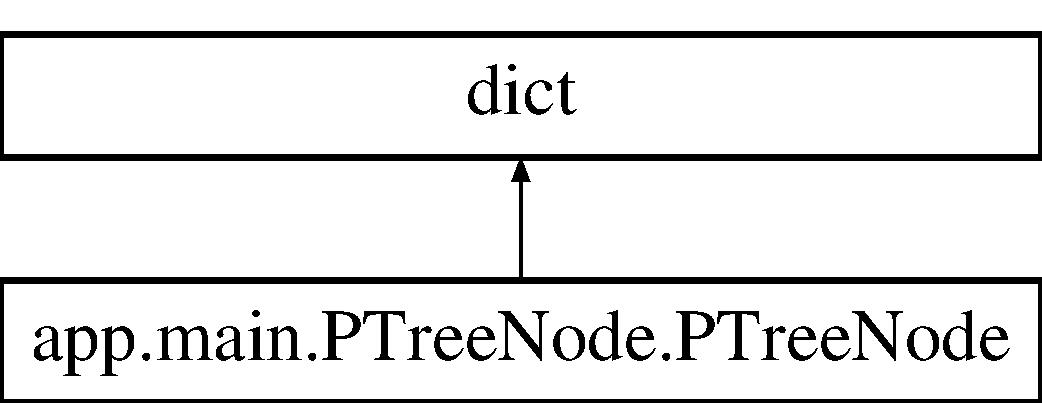
\includegraphics[height=2.000000cm]{classapp_1_1main_1_1PTreeNode_1_1PTreeNode}
\end{center}
\end{figure}
\subsection*{Public Member Functions}
\begin{DoxyCompactItemize}
\item 
\mbox{\Hypertarget{classapp_1_1main_1_1PTreeNode_1_1PTreeNode_abc830ac4a1b236b6a9261b2be3791e4b}\label{classapp_1_1main_1_1PTreeNode_1_1PTreeNode_abc830ac4a1b236b6a9261b2be3791e4b}} 
def {\bfseries \+\_\+\+\_\+init\+\_\+\+\_\+} (self, name, data=None, children=None, level=0)
\end{DoxyCompactItemize}
\subsection*{Public Attributes}
\begin{DoxyCompactItemize}
\item 
\mbox{\Hypertarget{classapp_1_1main_1_1PTreeNode_1_1PTreeNode_a5ae43a019e73e42ab9a5047068e66bbc}\label{classapp_1_1main_1_1PTreeNode_1_1PTreeNode_a5ae43a019e73e42ab9a5047068e66bbc}} 
{\bfseries name}
\item 
\mbox{\Hypertarget{classapp_1_1main_1_1PTreeNode_1_1PTreeNode_aac95bd54ab7f958f75c63a66c806b1e9}\label{classapp_1_1main_1_1PTreeNode_1_1PTreeNode_aac95bd54ab7f958f75c63a66c806b1e9}} 
{\bfseries data}
\item 
\mbox{\Hypertarget{classapp_1_1main_1_1PTreeNode_1_1PTreeNode_aae5eebe01363b149d66215e1646be328}\label{classapp_1_1main_1_1PTreeNode_1_1PTreeNode_aae5eebe01363b149d66215e1646be328}} 
{\bfseries level}
\item 
\mbox{\Hypertarget{classapp_1_1main_1_1PTreeNode_1_1PTreeNode_aba88e135fef7abf9cf91ae4dc16d5c9d}\label{classapp_1_1main_1_1PTreeNode_1_1PTreeNode_aba88e135fef7abf9cf91ae4dc16d5c9d}} 
{\bfseries children}
\end{DoxyCompactItemize}


\subsection{Detailed Description}
Purpose\+:Removes type info from name Arguments\+: 


\begin{DoxyParams}{Parameters}
{\em name} & \\
\hline
{\em data=\+None} & \\
\hline
{\em children=\+None} & \\
\hline
{\em level=0} & \\
\hline
\end{DoxyParams}


The documentation for this class was generated from the following file\+:\begin{DoxyCompactItemize}
\item 
/home/nlarsson/bbk/python/webdev/museumflask/app/main/\mbox{\hyperlink{PTreeNode_8py}{P\+Tree\+Node.\+py}}\end{DoxyCompactItemize}

\hypertarget{classapp_1_1main_1_1search_1_1Search}{}\section{app.\+main.\+search.\+Search Class Reference}
\label{classapp_1_1main_1_1search_1_1Search}\index{app.\+main.\+search.\+Search@{app.\+main.\+search.\+Search}}
\subsection*{Static Public Attributes}
\begin{DoxyCompactItemize}
\item 
\mbox{\Hypertarget{classapp_1_1main_1_1search_1_1Search_ac3c27e720804c176c2c14c3e02c02119}\label{classapp_1_1main_1_1search_1_1Search_ac3c27e720804c176c2c14c3e02c02119}} 
{\bfseries modeltoview} = \mbox{\hyperlink{classapp_1_1main_1_1model__to__view_1_1Model__To__View}{model\+\_\+to\+\_\+view.\+Model\+\_\+\+To\+\_\+\+View}}()
\end{DoxyCompactItemize}


The documentation for this class was generated from the following file\+:\begin{DoxyCompactItemize}
\item 
/home/nlarsson/bbk/python/webdev/museumflask/app/main/search.\+py\end{DoxyCompactItemize}

\hypertarget{classapp_1_1main_1_1showmuseumtypes_1_1ShowMuseumTypes}{}\section{app.\+main.\+showmuseumtypes.\+Show\+Museum\+Types Class Reference}
\label{classapp_1_1main_1_1showmuseumtypes_1_1ShowMuseumTypes}\index{app.\+main.\+showmuseumtypes.\+Show\+Museum\+Types@{app.\+main.\+showmuseumtypes.\+Show\+Museum\+Types}}
\subsection*{Static Public Attributes}
\begin{DoxyCompactItemize}
\item 
\mbox{\Hypertarget{classapp_1_1main_1_1showmuseumtypes_1_1ShowMuseumTypes_a935b43cbcf5b05ad54c3253b58dcc5a8}\label{classapp_1_1main_1_1showmuseumtypes_1_1ShowMuseumTypes_a935b43cbcf5b05ad54c3253b58dcc5a8}} 
{\bfseries dates}
\end{DoxyCompactItemize}


The documentation for this class was generated from the following file\+:\begin{DoxyCompactItemize}
\item 
/home/nlarsson/bbk/python/webdev/museumflask/app/main/showmuseumtypes.\+py\end{DoxyCompactItemize}

\hypertarget{classapp_1_1main_1_1boks_1_1Boks_1_1test__of__heatmap}{}\section{app.\+main.\+boks.\+Boks.\+test\+\_\+of\+\_\+heatmap Class Reference}
\label{classapp_1_1main_1_1boks_1_1Boks_1_1test__of__heatmap}\index{app.\+main.\+boks.\+Boks.\+test\+\_\+of\+\_\+heatmap@{app.\+main.\+boks.\+Boks.\+test\+\_\+of\+\_\+heatmap}}
\subsection*{Public Member Functions}
\begin{DoxyCompactItemize}
\item 
\mbox{\Hypertarget{classapp_1_1main_1_1boks_1_1Boks_1_1test__of__heatmap_a3ac125e18f531116c7d812114b9796b7}\label{classapp_1_1main_1_1boks_1_1Boks_1_1test__of__heatmap_a3ac125e18f531116c7d812114b9796b7}} 
def {\bfseries All} (self, me, parameters=None, contextdict=None)
\item 
\mbox{\Hypertarget{classapp_1_1main_1_1boks_1_1Boks_1_1test__of__heatmap_aa2875e15f2a7cace7df51f9c91b6b1e8}\label{classapp_1_1main_1_1boks_1_1Boks_1_1test__of__heatmap_aa2875e15f2a7cace7df51f9c91b6b1e8}} 
def {\bfseries Governance} (self, me, parameters=None, contextdict=None)
\item 
\mbox{\Hypertarget{classapp_1_1main_1_1boks_1_1Boks_1_1test__of__heatmap_a12953d53feb4de6296ded4734b9d6596}\label{classapp_1_1main_1_1boks_1_1Boks_1_1test__of__heatmap_a12953d53feb4de6296ded4734b9d6596}} 
def {\bfseries Subject\+\_\+\+Matter} (self, me, parameters=None, contextdict=None)
\item 
\mbox{\Hypertarget{classapp_1_1main_1_1boks_1_1Boks_1_1test__of__heatmap_adddb7abe4cb8a2d03a0dfaabfbbbd878}\label{classapp_1_1main_1_1boks_1_1Boks_1_1test__of__heatmap_adddb7abe4cb8a2d03a0dfaabfbbbd878}} 
def {\bfseries Size} (self, me, parameters=None, contextdict=None)
\item 
\mbox{\Hypertarget{classapp_1_1main_1_1boks_1_1Boks_1_1test__of__heatmap_a63231387dcade064cefec49faef6b158}\label{classapp_1_1main_1_1boks_1_1Boks_1_1test__of__heatmap_a63231387dcade064cefec49faef6b158}} 
def {\bfseries Location} (self, me, parameters=None, contextdict=None)
\end{DoxyCompactItemize}
\subsection*{Static Public Attributes}
\begin{DoxyCompactItemize}
\item 
\mbox{\Hypertarget{classapp_1_1main_1_1boks_1_1Boks_1_1test__of__heatmap_a20849fe82485fecf879d36da39fef282}\label{classapp_1_1main_1_1boks_1_1Boks_1_1test__of__heatmap_a20849fe82485fecf879d36da39fef282}} 
{\bfseries plot} = Boks.\+heat.\+create\+Plot(me,newparameters,contextdict)
\end{DoxyCompactItemize}


The documentation for this class was generated from the following file\+:\begin{DoxyCompactItemize}
\item 
/home/nlarsson/bbk/python/webdev/museumflask/app/main/\mbox{\hyperlink{boks_8py}{boks.\+py}}\end{DoxyCompactItemize}

\hypertarget{classapp_1_1main_1_1boks_1_1Boks_1_1that__opened__up__to__a__given__time}{}\section{app.\+main.\+boks.\+Boks.\+that\+\_\+opened\+\_\+up\+\_\+to\+\_\+a\+\_\+given\+\_\+time Class Reference}
\label{classapp_1_1main_1_1boks_1_1Boks_1_1that__opened__up__to__a__given__time}\index{app.\+main.\+boks.\+Boks.\+that\+\_\+opened\+\_\+up\+\_\+to\+\_\+a\+\_\+given\+\_\+time@{app.\+main.\+boks.\+Boks.\+that\+\_\+opened\+\_\+up\+\_\+to\+\_\+a\+\_\+given\+\_\+time}}
\subsection*{Public Member Functions}
\begin{DoxyCompactItemize}
\item 
\mbox{\Hypertarget{classapp_1_1main_1_1boks_1_1Boks_1_1that__opened__up__to__a__given__time_a5b61ca45cdc459a9e8ffa1bb5213df69}\label{classapp_1_1main_1_1boks_1_1Boks_1_1that__opened__up__to__a__given__time_a5b61ca45cdc459a9e8ffa1bb5213df69}} 
def {\bfseries Governance} (self, me, parameters=None, contextdict=None)
\item 
\mbox{\Hypertarget{classapp_1_1main_1_1boks_1_1Boks_1_1that__opened__up__to__a__given__time_ab0648859c120a48267a68a81a67fc949}\label{classapp_1_1main_1_1boks_1_1Boks_1_1that__opened__up__to__a__given__time_ab0648859c120a48267a68a81a67fc949}} 
def {\bfseries Subject\+\_\+\+Matter} (self, me, parameters=None, contextdict=None)
\item 
\mbox{\Hypertarget{classapp_1_1main_1_1boks_1_1Boks_1_1that__opened__up__to__a__given__time_a384136b8eb57c2381290604a7b145872}\label{classapp_1_1main_1_1boks_1_1Boks_1_1that__opened__up__to__a__given__time_a384136b8eb57c2381290604a7b145872}} 
def {\bfseries Size} (self, me, parameters=None, contextdict=None)
\item 
\mbox{\Hypertarget{classapp_1_1main_1_1boks_1_1Boks_1_1that__opened__up__to__a__given__time_afa594c5a19211b0639fd3dd680f73b34}\label{classapp_1_1main_1_1boks_1_1Boks_1_1that__opened__up__to__a__given__time_afa594c5a19211b0639fd3dd680f73b34}} 
def {\bfseries All} (self, me, parameters=None, contextdict=None)
\item 
\mbox{\Hypertarget{classapp_1_1main_1_1boks_1_1Boks_1_1that__opened__up__to__a__given__time_a9eb6512a8ed1e416b6b8f5bb34fabfdc}\label{classapp_1_1main_1_1boks_1_1Boks_1_1that__opened__up__to__a__given__time_a9eb6512a8ed1e416b6b8f5bb34fabfdc}} 
def {\bfseries Location} (self, me, parameters=None, contextdict=None)
\end{DoxyCompactItemize}
\subsection*{Static Public Attributes}
\begin{DoxyCompactItemize}
\item 
\mbox{\Hypertarget{classapp_1_1main_1_1boks_1_1Boks_1_1that__opened__up__to__a__given__time_aed54e5137afe5da4af18fa25bde4b7c1}\label{classapp_1_1main_1_1boks_1_1Boks_1_1that__opened__up__to__a__given__time_aed54e5137afe5da4af18fa25bde4b7c1}} 
{\bfseries plot} = Boks.\+categorybar.\+create\+Plot(me,newparameters,contextdict)
\end{DoxyCompactItemize}


The documentation for this class was generated from the following file\+:\begin{DoxyCompactItemize}
\item 
/home/nlarsson/bbk/python/webdev/museumflask/app/main/\mbox{\hyperlink{boks_8py}{boks.\+py}}\end{DoxyCompactItemize}

\hypertarget{classapp_1_1main_1_1treelib_1_1tree_1_1Tree}{}\section{app.\+main.\+treelib.\+tree.\+Tree Class Reference}
\label{classapp_1_1main_1_1treelib_1_1tree_1_1Tree}\index{app.\+main.\+treelib.\+tree.\+Tree@{app.\+main.\+treelib.\+tree.\+Tree}}
Inheritance diagram for app.\+main.\+treelib.\+tree.\+Tree\+:\begin{figure}[H]
\begin{center}
\leavevmode
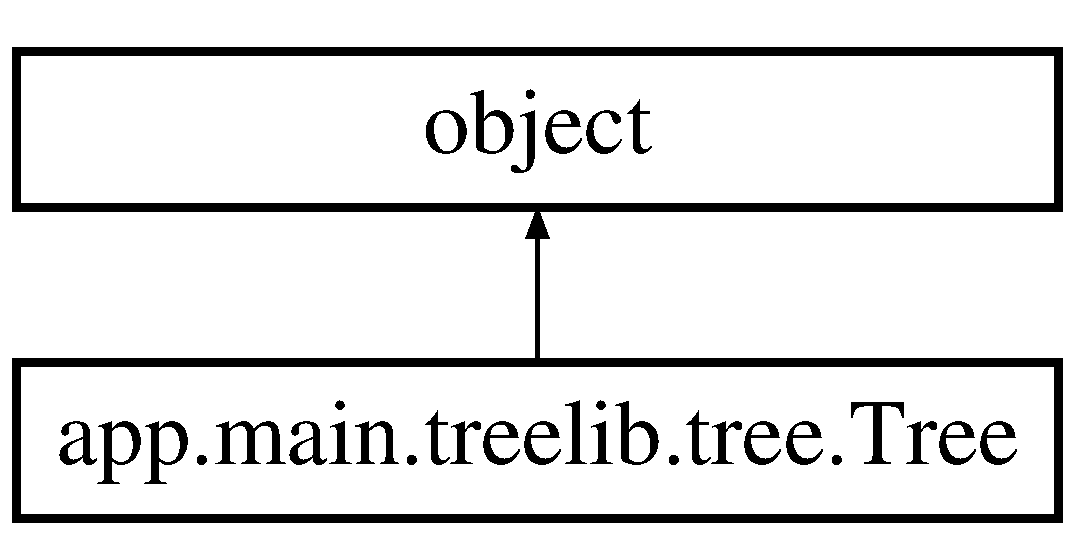
\includegraphics[height=2.000000cm]{classapp_1_1main_1_1treelib_1_1tree_1_1Tree}
\end{center}
\end{figure}
\subsection*{Public Member Functions}
\begin{DoxyCompactItemize}
\item 
def \mbox{\hyperlink{classapp_1_1main_1_1treelib_1_1tree_1_1Tree_a94e2233a52f68e21298a7dc78ed4c47a}{\+\_\+\+\_\+contains\+\_\+\+\_\+}} (self, identifier)
\item 
def \mbox{\hyperlink{classapp_1_1main_1_1treelib_1_1tree_1_1Tree_adb214f44cd20809a0d7568762680a210}{\+\_\+\+\_\+init\+\_\+\+\_\+}} (self, tree=None, deep=False)
\item 
def \mbox{\hyperlink{classapp_1_1main_1_1treelib_1_1tree_1_1Tree_a730e8bf6425ef9a60c0c1602b1469b73}{\+\_\+\+\_\+getitem\+\_\+\+\_\+}} (self, key)
\item 
def \mbox{\hyperlink{classapp_1_1main_1_1treelib_1_1tree_1_1Tree_a607c0dfb091a39681621b78cb32ab2d1}{\+\_\+\+\_\+len\+\_\+\+\_\+}} (self)
\item 
def \mbox{\hyperlink{classapp_1_1main_1_1treelib_1_1tree_1_1Tree_ab4e208b78bbfb1844201256aea101fb3}{\+\_\+\+\_\+setitem\+\_\+\+\_\+}} (self, key, item)
\item 
\mbox{\Hypertarget{classapp_1_1main_1_1treelib_1_1tree_1_1Tree_ac2c5d0ec2961121c92044d0f93543f7e}\label{classapp_1_1main_1_1treelib_1_1tree_1_1Tree_ac2c5d0ec2961121c92044d0f93543f7e}} 
def {\bfseries \+\_\+\+\_\+str\+\_\+\+\_\+} (self)
\item 
def \mbox{\hyperlink{classapp_1_1main_1_1treelib_1_1tree_1_1Tree_a8d9526231246f702318e9e1819868165}{add\+\_\+nodewithprefix}} (self, node, \mbox{\hyperlink{classapp_1_1main_1_1treelib_1_1tree_1_1Tree_a28ccb73f9aed492e66d879c664dc3b35}{parent}}=None, prefix=None)
\item 
def \mbox{\hyperlink{classapp_1_1main_1_1treelib_1_1tree_1_1Tree_a020b30ad1ff3cf947353487e75efcfc1}{add\+\_\+node}} (self, node, \mbox{\hyperlink{classapp_1_1main_1_1treelib_1_1tree_1_1Tree_a28ccb73f9aed492e66d879c664dc3b35}{parent}}=None)
\item 
def \mbox{\hyperlink{classapp_1_1main_1_1treelib_1_1tree_1_1Tree_a9d35f4e9e51cbccc98314ae78bb73a8f}{all\+\_\+nodes}} (self)
\item 
def \mbox{\hyperlink{classapp_1_1main_1_1treelib_1_1tree_1_1Tree_a6ec89f6f37ff6bee77e0c10d4270817c}{all\+\_\+nodes\+\_\+itr}} (self)
\item 
def \mbox{\hyperlink{classapp_1_1main_1_1treelib_1_1tree_1_1Tree_aa69c40af1b83aed2608bfaa4dedb6ff2}{children}} (self, nid)
\item 
def \mbox{\hyperlink{classapp_1_1main_1_1treelib_1_1tree_1_1Tree_aed85883a91c3bfe3e247115d041d42cc}{contains}} (self, nid)
\item 
def \mbox{\hyperlink{classapp_1_1main_1_1treelib_1_1tree_1_1Tree_a6bc326e192705fca6e6d71ea82fdcf57}{create\+\_\+node}} (self, tag=None, identifier=None, \mbox{\hyperlink{classapp_1_1main_1_1treelib_1_1tree_1_1Tree_a28ccb73f9aed492e66d879c664dc3b35}{parent}}=None, data=None)
\item 
def \mbox{\hyperlink{classapp_1_1main_1_1treelib_1_1tree_1_1Tree_a6ded8390652198c807e114ebe34692f6}{depth}} (self, node=None)
\item 
def \mbox{\hyperlink{classapp_1_1main_1_1treelib_1_1tree_1_1Tree_a5414ce6ec942fb619f8ff039113ffa16}{expand\+\_\+tree}} (self, nid=None, mode=D\+E\+P\+TH, filter=None, key=None, reverse=False)
\item 
def \mbox{\hyperlink{classapp_1_1main_1_1treelib_1_1tree_1_1Tree_a6c796bd0a0f6a97ddcaa4dc1808cd19e}{filter\+\_\+nodes}} (self, func)
\item 
def \mbox{\hyperlink{classapp_1_1main_1_1treelib_1_1tree_1_1Tree_a0eab04fe3e8c044a2c8c94a1d64e7fff}{get\+\_\+node}} (self, nid)
\item 
def \mbox{\hyperlink{classapp_1_1main_1_1treelib_1_1tree_1_1Tree_ad4d32e2665abec898618604bc706feaa}{is\+\_\+branch}} (self, nid)
\item 
def \mbox{\hyperlink{classapp_1_1main_1_1treelib_1_1tree_1_1Tree_a5ec4d13cd3bde4b97040c6e9bbf3253e}{leaves}} (self, nid=None)
\item 
def \mbox{\hyperlink{classapp_1_1main_1_1treelib_1_1tree_1_1Tree_a3d528173abf063f97e6dfbcf29a0564b}{level}} (self, nid, filter=None)
\item 
def \mbox{\hyperlink{classapp_1_1main_1_1treelib_1_1tree_1_1Tree_ae9fd733ebb27ca0f746951d1bb3ccd18}{link\+\_\+past\+\_\+node}} (self, nid)
\item 
def \mbox{\hyperlink{classapp_1_1main_1_1treelib_1_1tree_1_1Tree_a4663b9ae6dace6a5fb383e385ce46ac9}{move\+\_\+node}} (self, source, destination)
\item 
\mbox{\Hypertarget{classapp_1_1main_1_1treelib_1_1tree_1_1Tree_a7110650b43b794293ce278d1ce8ad106}\label{classapp_1_1main_1_1treelib_1_1tree_1_1Tree_a7110650b43b794293ce278d1ce8ad106}} 
def {\bfseries is\+\_\+ancestor} (self, ancestor, grandchild)
\item 
def \mbox{\hyperlink{classapp_1_1main_1_1treelib_1_1tree_1_1Tree_aa6848fc9aefc81193dcdda346b1d4e39}{nodes}} (self)
\item 
def \mbox{\hyperlink{classapp_1_1main_1_1treelib_1_1tree_1_1Tree_a28ccb73f9aed492e66d879c664dc3b35}{parent}} (self, nid)
\item 
\mbox{\Hypertarget{classapp_1_1main_1_1treelib_1_1tree_1_1Tree_a16215d893aaf0078bf5d5571aa62b778}\label{classapp_1_1main_1_1treelib_1_1tree_1_1Tree_a16215d893aaf0078bf5d5571aa62b778}} 
def {\bfseries count\+Children} (self, node)
\item 
\mbox{\Hypertarget{classapp_1_1main_1_1treelib_1_1tree_1_1Tree_ae89bf0c76e077786251d6687b43cfea0}\label{classapp_1_1main_1_1treelib_1_1tree_1_1Tree_ae89bf0c76e077786251d6687b43cfea0}} 
def {\bfseries has\+Child\+With\+Name} (self, node, name)
\item 
\mbox{\Hypertarget{classapp_1_1main_1_1treelib_1_1tree_1_1Tree_a45d3504fef6c6839b6190c122c55ca07}\label{classapp_1_1main_1_1treelib_1_1tree_1_1Tree_a45d3504fef6c6839b6190c122c55ca07}} 
def {\bfseries get\+Path\+For\+Node\+Ids} (self, node)
\item 
\mbox{\Hypertarget{classapp_1_1main_1_1treelib_1_1tree_1_1Tree_ac2cefd6987ad5ff487c00d7d95ff3a96}\label{classapp_1_1main_1_1treelib_1_1tree_1_1Tree_ac2cefd6987ad5ff487c00d7d95ff3a96}} 
def {\bfseries get\+Path\+For\+Node} (self, node)
\item 
def \mbox{\hyperlink{classapp_1_1main_1_1treelib_1_1tree_1_1Tree_a813bf6c69928f2004c0f1e04ce14e9b8}{paste}} (self, nid, new\+\_\+tree, deepcopy=False)
\item 
def \mbox{\hyperlink{classapp_1_1main_1_1treelib_1_1tree_1_1Tree_a0ce0cd39e8c6323cc9112b6f2325ffec}{paths\+\_\+to\+\_\+leaves}} (self)
\item 
def \mbox{\hyperlink{classapp_1_1main_1_1treelib_1_1tree_1_1Tree_ae560ce8ccbc05b3c7c70213606c64ae6}{remove\+\_\+node}} (self, identifier)
\item 
def \mbox{\hyperlink{classapp_1_1main_1_1treelib_1_1tree_1_1Tree_ad0f4edc203b3ea5d3bf5e77e2d8811e3}{remove\+\_\+subtree}} (self, nid)
\item 
def \mbox{\hyperlink{classapp_1_1main_1_1treelib_1_1tree_1_1Tree_a04080e6799c3bbc702b13953b466d757}{rsearch}} (self, nid, filter=None)
\item 
def \mbox{\hyperlink{classapp_1_1main_1_1treelib_1_1tree_1_1Tree_acfa08f527ee2152c58e090e3c5a698a1}{save2file}} (self, filename, nid=None, \mbox{\hyperlink{classapp_1_1main_1_1treelib_1_1tree_1_1Tree_a3d528173abf063f97e6dfbcf29a0564b}{level}}=R\+O\+OT, idhidden=True, filter=None, key=None, reverse=False, line\+\_\+type=\textquotesingle{}ascii-\/ex\textquotesingle{}, data\+\_\+property=None)
\item 
\mbox{\Hypertarget{classapp_1_1main_1_1treelib_1_1tree_1_1Tree_a8bb200b89d576eb8a0d077b1d9afe75f}\label{classapp_1_1main_1_1treelib_1_1tree_1_1Tree_a8bb200b89d576eb8a0d077b1d9afe75f}} 
def {\bfseries show} (self, nid=None, \mbox{\hyperlink{classapp_1_1main_1_1treelib_1_1tree_1_1Tree_a3d528173abf063f97e6dfbcf29a0564b}{level}}=R\+O\+OT, idhidden=True, filter=None, key=None, reverse=False, line\+\_\+type=\textquotesingle{}ascii-\/ex\textquotesingle{}, data\+\_\+property=None)
\item 
def \mbox{\hyperlink{classapp_1_1main_1_1treelib_1_1tree_1_1Tree_ad1ec030b369120a15221ee5b5b1b52e7}{siblings}} (self, nid)
\item 
def \mbox{\hyperlink{classapp_1_1main_1_1treelib_1_1tree_1_1Tree_ab647e277f063d1ad6ec236264d2a198f}{size}} (self, \mbox{\hyperlink{classapp_1_1main_1_1treelib_1_1tree_1_1Tree_a3d528173abf063f97e6dfbcf29a0564b}{level}}=None)
\item 
def \mbox{\hyperlink{classapp_1_1main_1_1treelib_1_1tree_1_1Tree_aed6f1044c77dbea0d03f2858e3a43eb4}{subtree}} (self, nid)
\item 
def \mbox{\hyperlink{classapp_1_1main_1_1treelib_1_1tree_1_1Tree_ad3d956786e8d7e468425d15dcdd929d0}{to\+\_\+dict}} (self, nid=None, key=None, sort=True, reverse=False, with\+\_\+data=False)
\item 
def \mbox{\hyperlink{classapp_1_1main_1_1treelib_1_1tree_1_1Tree_aa2a265f8990cbd53fbf80f5ef5b49b20}{to\+\_\+json}} (self, with\+\_\+data=False, sort=True, reverse=False)
\item 
def \mbox{\hyperlink{classapp_1_1main_1_1treelib_1_1tree_1_1Tree_a2cdb045aff10eb712ef0109997553a25}{update\+\_\+node}} (self, nid, attrs)
\end{DoxyCompactItemize}
\subsection*{Public Attributes}
\begin{DoxyCompactItemize}
\item 
\mbox{\Hypertarget{classapp_1_1main_1_1treelib_1_1tree_1_1Tree_a906fd88dfeeffa2729b9a2f5ab01d36d}\label{classapp_1_1main_1_1treelib_1_1tree_1_1Tree_a906fd88dfeeffa2729b9a2f5ab01d36d}} 
{\bfseries root}
\end{DoxyCompactItemize}
\subsection*{Static Public Attributes}
\begin{DoxyCompactItemize}
\item 
\mbox{\Hypertarget{classapp_1_1main_1_1treelib_1_1tree_1_1Tree_a21ee57e8d7abc87b9edf7f0f4d5c7a11}\label{classapp_1_1main_1_1treelib_1_1tree_1_1Tree_a21ee57e8d7abc87b9edf7f0f4d5c7a11}} 
{\bfseries count}
\item 
\mbox{\Hypertarget{classapp_1_1main_1_1treelib_1_1tree_1_1Tree_a3abae45851124cd925789ffc4e914b40}\label{classapp_1_1main_1_1treelib_1_1tree_1_1Tree_a3abae45851124cd925789ffc4e914b40}} 
{\bfseries children}
\end{DoxyCompactItemize}


\subsection{Detailed Description}
\begin{DoxyVerb}Tree objects are made of Node(s) stored in _nodes dictionary.\end{DoxyVerb}
 

\subsection{Constructor \& Destructor Documentation}
\mbox{\Hypertarget{classapp_1_1main_1_1treelib_1_1tree_1_1Tree_adb214f44cd20809a0d7568762680a210}\label{classapp_1_1main_1_1treelib_1_1tree_1_1Tree_adb214f44cd20809a0d7568762680a210}} 
\index{app\+::main\+::treelib\+::tree\+::\+Tree@{app\+::main\+::treelib\+::tree\+::\+Tree}!\+\_\+\+\_\+init\+\_\+\+\_\+@{\+\_\+\+\_\+init\+\_\+\+\_\+}}
\index{\+\_\+\+\_\+init\+\_\+\+\_\+@{\+\_\+\+\_\+init\+\_\+\+\_\+}!app\+::main\+::treelib\+::tree\+::\+Tree@{app\+::main\+::treelib\+::tree\+::\+Tree}}
\subsubsection{\texorpdfstring{\+\_\+\+\_\+init\+\_\+\+\_\+()}{\_\_init\_\_()}}
{\footnotesize\ttfamily def app.\+main.\+treelib.\+tree.\+Tree.\+\_\+\+\_\+init\+\_\+\+\_\+ (\begin{DoxyParamCaption}\item[{}]{self,  }\item[{}]{tree = {\ttfamily None},  }\item[{}]{deep = {\ttfamily False} }\end{DoxyParamCaption})}

\begin{DoxyVerb}Initiate a new tree or copy another tree with a shallow or
deep copy.
\end{DoxyVerb}
 

\subsection{Member Function Documentation}
\mbox{\Hypertarget{classapp_1_1main_1_1treelib_1_1tree_1_1Tree_a94e2233a52f68e21298a7dc78ed4c47a}\label{classapp_1_1main_1_1treelib_1_1tree_1_1Tree_a94e2233a52f68e21298a7dc78ed4c47a}} 
\index{app\+::main\+::treelib\+::tree\+::\+Tree@{app\+::main\+::treelib\+::tree\+::\+Tree}!\+\_\+\+\_\+contains\+\_\+\+\_\+@{\+\_\+\+\_\+contains\+\_\+\+\_\+}}
\index{\+\_\+\+\_\+contains\+\_\+\+\_\+@{\+\_\+\+\_\+contains\+\_\+\+\_\+}!app\+::main\+::treelib\+::tree\+::\+Tree@{app\+::main\+::treelib\+::tree\+::\+Tree}}
\subsubsection{\texorpdfstring{\+\_\+\+\_\+contains\+\_\+\+\_\+()}{\_\_contains\_\_()}}
{\footnotesize\ttfamily def app.\+main.\+treelib.\+tree.\+Tree.\+\_\+\+\_\+contains\+\_\+\+\_\+ (\begin{DoxyParamCaption}\item[{}]{self,  }\item[{}]{identifier }\end{DoxyParamCaption})}

\begin{DoxyVerb}Return a list of the nodes'identifiers matching the
identifier argument.
\end{DoxyVerb}
 \mbox{\Hypertarget{classapp_1_1main_1_1treelib_1_1tree_1_1Tree_a730e8bf6425ef9a60c0c1602b1469b73}\label{classapp_1_1main_1_1treelib_1_1tree_1_1Tree_a730e8bf6425ef9a60c0c1602b1469b73}} 
\index{app\+::main\+::treelib\+::tree\+::\+Tree@{app\+::main\+::treelib\+::tree\+::\+Tree}!\+\_\+\+\_\+getitem\+\_\+\+\_\+@{\+\_\+\+\_\+getitem\+\_\+\+\_\+}}
\index{\+\_\+\+\_\+getitem\+\_\+\+\_\+@{\+\_\+\+\_\+getitem\+\_\+\+\_\+}!app\+::main\+::treelib\+::tree\+::\+Tree@{app\+::main\+::treelib\+::tree\+::\+Tree}}
\subsubsection{\texorpdfstring{\+\_\+\+\_\+getitem\+\_\+\+\_\+()}{\_\_getitem\_\_()}}
{\footnotesize\ttfamily def app.\+main.\+treelib.\+tree.\+Tree.\+\_\+\+\_\+getitem\+\_\+\+\_\+ (\begin{DoxyParamCaption}\item[{}]{self,  }\item[{}]{key }\end{DoxyParamCaption})}

\begin{DoxyVerb}Return _nodes[key]\end{DoxyVerb}
 \mbox{\Hypertarget{classapp_1_1main_1_1treelib_1_1tree_1_1Tree_a607c0dfb091a39681621b78cb32ab2d1}\label{classapp_1_1main_1_1treelib_1_1tree_1_1Tree_a607c0dfb091a39681621b78cb32ab2d1}} 
\index{app\+::main\+::treelib\+::tree\+::\+Tree@{app\+::main\+::treelib\+::tree\+::\+Tree}!\+\_\+\+\_\+len\+\_\+\+\_\+@{\+\_\+\+\_\+len\+\_\+\+\_\+}}
\index{\+\_\+\+\_\+len\+\_\+\+\_\+@{\+\_\+\+\_\+len\+\_\+\+\_\+}!app\+::main\+::treelib\+::tree\+::\+Tree@{app\+::main\+::treelib\+::tree\+::\+Tree}}
\subsubsection{\texorpdfstring{\+\_\+\+\_\+len\+\_\+\+\_\+()}{\_\_len\_\_()}}
{\footnotesize\ttfamily def app.\+main.\+treelib.\+tree.\+Tree.\+\_\+\+\_\+len\+\_\+\+\_\+ (\begin{DoxyParamCaption}\item[{}]{self }\end{DoxyParamCaption})}

\begin{DoxyVerb}Return len(_nodes)\end{DoxyVerb}
 \mbox{\Hypertarget{classapp_1_1main_1_1treelib_1_1tree_1_1Tree_ab4e208b78bbfb1844201256aea101fb3}\label{classapp_1_1main_1_1treelib_1_1tree_1_1Tree_ab4e208b78bbfb1844201256aea101fb3}} 
\index{app\+::main\+::treelib\+::tree\+::\+Tree@{app\+::main\+::treelib\+::tree\+::\+Tree}!\+\_\+\+\_\+setitem\+\_\+\+\_\+@{\+\_\+\+\_\+setitem\+\_\+\+\_\+}}
\index{\+\_\+\+\_\+setitem\+\_\+\+\_\+@{\+\_\+\+\_\+setitem\+\_\+\+\_\+}!app\+::main\+::treelib\+::tree\+::\+Tree@{app\+::main\+::treelib\+::tree\+::\+Tree}}
\subsubsection{\texorpdfstring{\+\_\+\+\_\+setitem\+\_\+\+\_\+()}{\_\_setitem\_\_()}}
{\footnotesize\ttfamily def app.\+main.\+treelib.\+tree.\+Tree.\+\_\+\+\_\+setitem\+\_\+\+\_\+ (\begin{DoxyParamCaption}\item[{}]{self,  }\item[{}]{key,  }\item[{}]{item }\end{DoxyParamCaption})}

\begin{DoxyVerb}Set _nodes[key]\end{DoxyVerb}
 \mbox{\Hypertarget{classapp_1_1main_1_1treelib_1_1tree_1_1Tree_a020b30ad1ff3cf947353487e75efcfc1}\label{classapp_1_1main_1_1treelib_1_1tree_1_1Tree_a020b30ad1ff3cf947353487e75efcfc1}} 
\index{app\+::main\+::treelib\+::tree\+::\+Tree@{app\+::main\+::treelib\+::tree\+::\+Tree}!add\+\_\+node@{add\+\_\+node}}
\index{add\+\_\+node@{add\+\_\+node}!app\+::main\+::treelib\+::tree\+::\+Tree@{app\+::main\+::treelib\+::tree\+::\+Tree}}
\subsubsection{\texorpdfstring{add\+\_\+node()}{add\_node()}}
{\footnotesize\ttfamily def app.\+main.\+treelib.\+tree.\+Tree.\+add\+\_\+node (\begin{DoxyParamCaption}\item[{}]{self,  }\item[{}]{node,  }\item[{}]{parent = {\ttfamily None} }\end{DoxyParamCaption})}

\begin{DoxyVerb}Add a new node to tree.
The 'node' parameter refers to an instance of Class::Node
\end{DoxyVerb}
 \mbox{\Hypertarget{classapp_1_1main_1_1treelib_1_1tree_1_1Tree_a8d9526231246f702318e9e1819868165}\label{classapp_1_1main_1_1treelib_1_1tree_1_1Tree_a8d9526231246f702318e9e1819868165}} 
\index{app\+::main\+::treelib\+::tree\+::\+Tree@{app\+::main\+::treelib\+::tree\+::\+Tree}!add\+\_\+nodewithprefix@{add\+\_\+nodewithprefix}}
\index{add\+\_\+nodewithprefix@{add\+\_\+nodewithprefix}!app\+::main\+::treelib\+::tree\+::\+Tree@{app\+::main\+::treelib\+::tree\+::\+Tree}}
\subsubsection{\texorpdfstring{add\+\_\+nodewithprefix()}{add\_nodewithprefix()}}
{\footnotesize\ttfamily def app.\+main.\+treelib.\+tree.\+Tree.\+add\+\_\+nodewithprefix (\begin{DoxyParamCaption}\item[{}]{self,  }\item[{}]{node,  }\item[{}]{parent = {\ttfamily None},  }\item[{}]{prefix = {\ttfamily None} }\end{DoxyParamCaption})}

\begin{DoxyVerb}Add a new node to tree.
The 'node' parameter refers to an instance of Class::Node
\end{DoxyVerb}
 \mbox{\Hypertarget{classapp_1_1main_1_1treelib_1_1tree_1_1Tree_a9d35f4e9e51cbccc98314ae78bb73a8f}\label{classapp_1_1main_1_1treelib_1_1tree_1_1Tree_a9d35f4e9e51cbccc98314ae78bb73a8f}} 
\index{app\+::main\+::treelib\+::tree\+::\+Tree@{app\+::main\+::treelib\+::tree\+::\+Tree}!all\+\_\+nodes@{all\+\_\+nodes}}
\index{all\+\_\+nodes@{all\+\_\+nodes}!app\+::main\+::treelib\+::tree\+::\+Tree@{app\+::main\+::treelib\+::tree\+::\+Tree}}
\subsubsection{\texorpdfstring{all\+\_\+nodes()}{all\_nodes()}}
{\footnotesize\ttfamily def app.\+main.\+treelib.\+tree.\+Tree.\+all\+\_\+nodes (\begin{DoxyParamCaption}\item[{}]{self }\end{DoxyParamCaption})}

\begin{DoxyVerb}Return all nodes in a list\end{DoxyVerb}
 \mbox{\Hypertarget{classapp_1_1main_1_1treelib_1_1tree_1_1Tree_a6ec89f6f37ff6bee77e0c10d4270817c}\label{classapp_1_1main_1_1treelib_1_1tree_1_1Tree_a6ec89f6f37ff6bee77e0c10d4270817c}} 
\index{app\+::main\+::treelib\+::tree\+::\+Tree@{app\+::main\+::treelib\+::tree\+::\+Tree}!all\+\_\+nodes\+\_\+itr@{all\+\_\+nodes\+\_\+itr}}
\index{all\+\_\+nodes\+\_\+itr@{all\+\_\+nodes\+\_\+itr}!app\+::main\+::treelib\+::tree\+::\+Tree@{app\+::main\+::treelib\+::tree\+::\+Tree}}
\subsubsection{\texorpdfstring{all\+\_\+nodes\+\_\+itr()}{all\_nodes\_itr()}}
{\footnotesize\ttfamily def app.\+main.\+treelib.\+tree.\+Tree.\+all\+\_\+nodes\+\_\+itr (\begin{DoxyParamCaption}\item[{}]{self }\end{DoxyParamCaption})}

\begin{DoxyVerb}Returns all nodes in an iterator
Added by William Rusnack
\end{DoxyVerb}
 \mbox{\Hypertarget{classapp_1_1main_1_1treelib_1_1tree_1_1Tree_aa69c40af1b83aed2608bfaa4dedb6ff2}\label{classapp_1_1main_1_1treelib_1_1tree_1_1Tree_aa69c40af1b83aed2608bfaa4dedb6ff2}} 
\index{app\+::main\+::treelib\+::tree\+::\+Tree@{app\+::main\+::treelib\+::tree\+::\+Tree}!children@{children}}
\index{children@{children}!app\+::main\+::treelib\+::tree\+::\+Tree@{app\+::main\+::treelib\+::tree\+::\+Tree}}
\subsubsection{\texorpdfstring{children()}{children()}}
{\footnotesize\ttfamily def app.\+main.\+treelib.\+tree.\+Tree.\+children (\begin{DoxyParamCaption}\item[{}]{self,  }\item[{}]{nid }\end{DoxyParamCaption})}

\begin{DoxyVerb}Return the children (Node) list of nid.
Empty list is returned if nid does not exist
\end{DoxyVerb}
 \mbox{\Hypertarget{classapp_1_1main_1_1treelib_1_1tree_1_1Tree_aed85883a91c3bfe3e247115d041d42cc}\label{classapp_1_1main_1_1treelib_1_1tree_1_1Tree_aed85883a91c3bfe3e247115d041d42cc}} 
\index{app\+::main\+::treelib\+::tree\+::\+Tree@{app\+::main\+::treelib\+::tree\+::\+Tree}!contains@{contains}}
\index{contains@{contains}!app\+::main\+::treelib\+::tree\+::\+Tree@{app\+::main\+::treelib\+::tree\+::\+Tree}}
\subsubsection{\texorpdfstring{contains()}{contains()}}
{\footnotesize\ttfamily def app.\+main.\+treelib.\+tree.\+Tree.\+contains (\begin{DoxyParamCaption}\item[{}]{self,  }\item[{}]{nid }\end{DoxyParamCaption})}

\begin{DoxyVerb}Check if the tree contains node of given id\end{DoxyVerb}
 \mbox{\Hypertarget{classapp_1_1main_1_1treelib_1_1tree_1_1Tree_a6bc326e192705fca6e6d71ea82fdcf57}\label{classapp_1_1main_1_1treelib_1_1tree_1_1Tree_a6bc326e192705fca6e6d71ea82fdcf57}} 
\index{app\+::main\+::treelib\+::tree\+::\+Tree@{app\+::main\+::treelib\+::tree\+::\+Tree}!create\+\_\+node@{create\+\_\+node}}
\index{create\+\_\+node@{create\+\_\+node}!app\+::main\+::treelib\+::tree\+::\+Tree@{app\+::main\+::treelib\+::tree\+::\+Tree}}
\subsubsection{\texorpdfstring{create\+\_\+node()}{create\_node()}}
{\footnotesize\ttfamily def app.\+main.\+treelib.\+tree.\+Tree.\+create\+\_\+node (\begin{DoxyParamCaption}\item[{}]{self,  }\item[{}]{tag = {\ttfamily None},  }\item[{}]{identifier = {\ttfamily None},  }\item[{}]{parent = {\ttfamily None},  }\item[{}]{data = {\ttfamily None} }\end{DoxyParamCaption})}

\begin{DoxyVerb}Create a child node for given @parent node.\end{DoxyVerb}
 \mbox{\Hypertarget{classapp_1_1main_1_1treelib_1_1tree_1_1Tree_a6ded8390652198c807e114ebe34692f6}\label{classapp_1_1main_1_1treelib_1_1tree_1_1Tree_a6ded8390652198c807e114ebe34692f6}} 
\index{app\+::main\+::treelib\+::tree\+::\+Tree@{app\+::main\+::treelib\+::tree\+::\+Tree}!depth@{depth}}
\index{depth@{depth}!app\+::main\+::treelib\+::tree\+::\+Tree@{app\+::main\+::treelib\+::tree\+::\+Tree}}
\subsubsection{\texorpdfstring{depth()}{depth()}}
{\footnotesize\ttfamily def app.\+main.\+treelib.\+tree.\+Tree.\+depth (\begin{DoxyParamCaption}\item[{}]{self,  }\item[{}]{node = {\ttfamily None} }\end{DoxyParamCaption})}

\begin{DoxyVerb}Get the maximum level of this tree or the level of the given node

@param node Node instance or identifier
@return int
@throw NodeIDAbsentError
\end{DoxyVerb}
 \mbox{\Hypertarget{classapp_1_1main_1_1treelib_1_1tree_1_1Tree_a5414ce6ec942fb619f8ff039113ffa16}\label{classapp_1_1main_1_1treelib_1_1tree_1_1Tree_a5414ce6ec942fb619f8ff039113ffa16}} 
\index{app\+::main\+::treelib\+::tree\+::\+Tree@{app\+::main\+::treelib\+::tree\+::\+Tree}!expand\+\_\+tree@{expand\+\_\+tree}}
\index{expand\+\_\+tree@{expand\+\_\+tree}!app\+::main\+::treelib\+::tree\+::\+Tree@{app\+::main\+::treelib\+::tree\+::\+Tree}}
\subsubsection{\texorpdfstring{expand\+\_\+tree()}{expand\_tree()}}
{\footnotesize\ttfamily def app.\+main.\+treelib.\+tree.\+Tree.\+expand\+\_\+tree (\begin{DoxyParamCaption}\item[{}]{self,  }\item[{}]{nid = {\ttfamily None},  }\item[{}]{mode = {\ttfamily DEPTH},  }\item[{}]{filter = {\ttfamily None},  }\item[{}]{key = {\ttfamily None},  }\item[{}]{reverse = {\ttfamily False} }\end{DoxyParamCaption})}

\begin{DoxyVerb}Python generator. Loosly based on an algorithm from
'Essential LISP' by John R. Anderson, Albert T. Corbett, and
Brian J. Reiser, page 239-241

UPDATE: the @filter function is performed on Node object during
traversing. In this manner, the traversing will not continue to
following children of node whose condition does not pass the filter.

UPDATE: the @key and @reverse are present to sort nodes at each
level.
\end{DoxyVerb}
 \mbox{\Hypertarget{classapp_1_1main_1_1treelib_1_1tree_1_1Tree_a6c796bd0a0f6a97ddcaa4dc1808cd19e}\label{classapp_1_1main_1_1treelib_1_1tree_1_1Tree_a6c796bd0a0f6a97ddcaa4dc1808cd19e}} 
\index{app\+::main\+::treelib\+::tree\+::\+Tree@{app\+::main\+::treelib\+::tree\+::\+Tree}!filter\+\_\+nodes@{filter\+\_\+nodes}}
\index{filter\+\_\+nodes@{filter\+\_\+nodes}!app\+::main\+::treelib\+::tree\+::\+Tree@{app\+::main\+::treelib\+::tree\+::\+Tree}}
\subsubsection{\texorpdfstring{filter\+\_\+nodes()}{filter\_nodes()}}
{\footnotesize\ttfamily def app.\+main.\+treelib.\+tree.\+Tree.\+filter\+\_\+nodes (\begin{DoxyParamCaption}\item[{}]{self,  }\item[{}]{func }\end{DoxyParamCaption})}

\begin{DoxyVerb}Filters all nodes by function
function is passed one node as an argument and that node is included if function returns true
returns a filter iterator of the node in python 3 or a list of the nodes in python 2
Added William Rusnack
\end{DoxyVerb}
 \mbox{\Hypertarget{classapp_1_1main_1_1treelib_1_1tree_1_1Tree_a0eab04fe3e8c044a2c8c94a1d64e7fff}\label{classapp_1_1main_1_1treelib_1_1tree_1_1Tree_a0eab04fe3e8c044a2c8c94a1d64e7fff}} 
\index{app\+::main\+::treelib\+::tree\+::\+Tree@{app\+::main\+::treelib\+::tree\+::\+Tree}!get\+\_\+node@{get\+\_\+node}}
\index{get\+\_\+node@{get\+\_\+node}!app\+::main\+::treelib\+::tree\+::\+Tree@{app\+::main\+::treelib\+::tree\+::\+Tree}}
\subsubsection{\texorpdfstring{get\+\_\+node()}{get\_node()}}
{\footnotesize\ttfamily def app.\+main.\+treelib.\+tree.\+Tree.\+get\+\_\+node (\begin{DoxyParamCaption}\item[{}]{self,  }\item[{}]{nid }\end{DoxyParamCaption})}

\begin{DoxyVerb}Return the node with `nid`. None returned if `nid` does not exist.\end{DoxyVerb}
 \mbox{\Hypertarget{classapp_1_1main_1_1treelib_1_1tree_1_1Tree_ad4d32e2665abec898618604bc706feaa}\label{classapp_1_1main_1_1treelib_1_1tree_1_1Tree_ad4d32e2665abec898618604bc706feaa}} 
\index{app\+::main\+::treelib\+::tree\+::\+Tree@{app\+::main\+::treelib\+::tree\+::\+Tree}!is\+\_\+branch@{is\+\_\+branch}}
\index{is\+\_\+branch@{is\+\_\+branch}!app\+::main\+::treelib\+::tree\+::\+Tree@{app\+::main\+::treelib\+::tree\+::\+Tree}}
\subsubsection{\texorpdfstring{is\+\_\+branch()}{is\_branch()}}
{\footnotesize\ttfamily def app.\+main.\+treelib.\+tree.\+Tree.\+is\+\_\+branch (\begin{DoxyParamCaption}\item[{}]{self,  }\item[{}]{nid }\end{DoxyParamCaption})}

\begin{DoxyVerb}Return the children (ID) list of nid.
Empty list is returned if nid does not exist
\end{DoxyVerb}
 \mbox{\Hypertarget{classapp_1_1main_1_1treelib_1_1tree_1_1Tree_a5ec4d13cd3bde4b97040c6e9bbf3253e}\label{classapp_1_1main_1_1treelib_1_1tree_1_1Tree_a5ec4d13cd3bde4b97040c6e9bbf3253e}} 
\index{app\+::main\+::treelib\+::tree\+::\+Tree@{app\+::main\+::treelib\+::tree\+::\+Tree}!leaves@{leaves}}
\index{leaves@{leaves}!app\+::main\+::treelib\+::tree\+::\+Tree@{app\+::main\+::treelib\+::tree\+::\+Tree}}
\subsubsection{\texorpdfstring{leaves()}{leaves()}}
{\footnotesize\ttfamily def app.\+main.\+treelib.\+tree.\+Tree.\+leaves (\begin{DoxyParamCaption}\item[{}]{self,  }\item[{}]{nid = {\ttfamily None} }\end{DoxyParamCaption})}

\begin{DoxyVerb}Get leaves of the whole tree of a subtree.\end{DoxyVerb}
 \mbox{\Hypertarget{classapp_1_1main_1_1treelib_1_1tree_1_1Tree_a3d528173abf063f97e6dfbcf29a0564b}\label{classapp_1_1main_1_1treelib_1_1tree_1_1Tree_a3d528173abf063f97e6dfbcf29a0564b}} 
\index{app\+::main\+::treelib\+::tree\+::\+Tree@{app\+::main\+::treelib\+::tree\+::\+Tree}!level@{level}}
\index{level@{level}!app\+::main\+::treelib\+::tree\+::\+Tree@{app\+::main\+::treelib\+::tree\+::\+Tree}}
\subsubsection{\texorpdfstring{level()}{level()}}
{\footnotesize\ttfamily def app.\+main.\+treelib.\+tree.\+Tree.\+level (\begin{DoxyParamCaption}\item[{}]{self,  }\item[{}]{nid,  }\item[{}]{filter = {\ttfamily None} }\end{DoxyParamCaption})}

\begin{DoxyVerb}Get the node level in this tree.
The level is an integer starting with '0' at the root.
In other words, the root lives at level '0';

Update: @filter params is added to calculate level passing
exclusive nodes.
\end{DoxyVerb}
 \mbox{\Hypertarget{classapp_1_1main_1_1treelib_1_1tree_1_1Tree_ae9fd733ebb27ca0f746951d1bb3ccd18}\label{classapp_1_1main_1_1treelib_1_1tree_1_1Tree_ae9fd733ebb27ca0f746951d1bb3ccd18}} 
\index{app\+::main\+::treelib\+::tree\+::\+Tree@{app\+::main\+::treelib\+::tree\+::\+Tree}!link\+\_\+past\+\_\+node@{link\+\_\+past\+\_\+node}}
\index{link\+\_\+past\+\_\+node@{link\+\_\+past\+\_\+node}!app\+::main\+::treelib\+::tree\+::\+Tree@{app\+::main\+::treelib\+::tree\+::\+Tree}}
\subsubsection{\texorpdfstring{link\+\_\+past\+\_\+node()}{link\_past\_node()}}
{\footnotesize\ttfamily def app.\+main.\+treelib.\+tree.\+Tree.\+link\+\_\+past\+\_\+node (\begin{DoxyParamCaption}\item[{}]{self,  }\item[{}]{nid }\end{DoxyParamCaption})}

\begin{DoxyVerb}Delete a node by linking past it.

For example, if we have a -> b -> c and delete node b, we are left
with a -> c
\end{DoxyVerb}
 \mbox{\Hypertarget{classapp_1_1main_1_1treelib_1_1tree_1_1Tree_a4663b9ae6dace6a5fb383e385ce46ac9}\label{classapp_1_1main_1_1treelib_1_1tree_1_1Tree_a4663b9ae6dace6a5fb383e385ce46ac9}} 
\index{app\+::main\+::treelib\+::tree\+::\+Tree@{app\+::main\+::treelib\+::tree\+::\+Tree}!move\+\_\+node@{move\+\_\+node}}
\index{move\+\_\+node@{move\+\_\+node}!app\+::main\+::treelib\+::tree\+::\+Tree@{app\+::main\+::treelib\+::tree\+::\+Tree}}
\subsubsection{\texorpdfstring{move\+\_\+node()}{move\_node()}}
{\footnotesize\ttfamily def app.\+main.\+treelib.\+tree.\+Tree.\+move\+\_\+node (\begin{DoxyParamCaption}\item[{}]{self,  }\item[{}]{source,  }\item[{}]{destination }\end{DoxyParamCaption})}

\begin{DoxyVerb}Move a node indicated by @source parameter to be a child of
@destination.
\end{DoxyVerb}
 \mbox{\Hypertarget{classapp_1_1main_1_1treelib_1_1tree_1_1Tree_aa6848fc9aefc81193dcdda346b1d4e39}\label{classapp_1_1main_1_1treelib_1_1tree_1_1Tree_aa6848fc9aefc81193dcdda346b1d4e39}} 
\index{app\+::main\+::treelib\+::tree\+::\+Tree@{app\+::main\+::treelib\+::tree\+::\+Tree}!nodes@{nodes}}
\index{nodes@{nodes}!app\+::main\+::treelib\+::tree\+::\+Tree@{app\+::main\+::treelib\+::tree\+::\+Tree}}
\subsubsection{\texorpdfstring{nodes()}{nodes()}}
{\footnotesize\ttfamily def app.\+main.\+treelib.\+tree.\+Tree.\+nodes (\begin{DoxyParamCaption}\item[{}]{self }\end{DoxyParamCaption})}

\begin{DoxyVerb}Return a dict form of nodes in a tree: {id: node_instance}\end{DoxyVerb}
 \mbox{\Hypertarget{classapp_1_1main_1_1treelib_1_1tree_1_1Tree_a28ccb73f9aed492e66d879c664dc3b35}\label{classapp_1_1main_1_1treelib_1_1tree_1_1Tree_a28ccb73f9aed492e66d879c664dc3b35}} 
\index{app\+::main\+::treelib\+::tree\+::\+Tree@{app\+::main\+::treelib\+::tree\+::\+Tree}!parent@{parent}}
\index{parent@{parent}!app\+::main\+::treelib\+::tree\+::\+Tree@{app\+::main\+::treelib\+::tree\+::\+Tree}}
\subsubsection{\texorpdfstring{parent()}{parent()}}
{\footnotesize\ttfamily def app.\+main.\+treelib.\+tree.\+Tree.\+parent (\begin{DoxyParamCaption}\item[{}]{self,  }\item[{}]{nid }\end{DoxyParamCaption})}

\begin{DoxyVerb}Get parent node object of given id\end{DoxyVerb}
 \mbox{\Hypertarget{classapp_1_1main_1_1treelib_1_1tree_1_1Tree_a813bf6c69928f2004c0f1e04ce14e9b8}\label{classapp_1_1main_1_1treelib_1_1tree_1_1Tree_a813bf6c69928f2004c0f1e04ce14e9b8}} 
\index{app\+::main\+::treelib\+::tree\+::\+Tree@{app\+::main\+::treelib\+::tree\+::\+Tree}!paste@{paste}}
\index{paste@{paste}!app\+::main\+::treelib\+::tree\+::\+Tree@{app\+::main\+::treelib\+::tree\+::\+Tree}}
\subsubsection{\texorpdfstring{paste()}{paste()}}
{\footnotesize\ttfamily def app.\+main.\+treelib.\+tree.\+Tree.\+paste (\begin{DoxyParamCaption}\item[{}]{self,  }\item[{}]{nid,  }\item[{}]{new\+\_\+tree,  }\item[{}]{deepcopy = {\ttfamily False} }\end{DoxyParamCaption})}

\begin{DoxyVerb}Paste a @new_tree to the original one by linking the root
of new tree to given node (nid).

Update: add @deepcopy of pasted tree.
\end{DoxyVerb}
 \mbox{\Hypertarget{classapp_1_1main_1_1treelib_1_1tree_1_1Tree_a0ce0cd39e8c6323cc9112b6f2325ffec}\label{classapp_1_1main_1_1treelib_1_1tree_1_1Tree_a0ce0cd39e8c6323cc9112b6f2325ffec}} 
\index{app\+::main\+::treelib\+::tree\+::\+Tree@{app\+::main\+::treelib\+::tree\+::\+Tree}!paths\+\_\+to\+\_\+leaves@{paths\+\_\+to\+\_\+leaves}}
\index{paths\+\_\+to\+\_\+leaves@{paths\+\_\+to\+\_\+leaves}!app\+::main\+::treelib\+::tree\+::\+Tree@{app\+::main\+::treelib\+::tree\+::\+Tree}}
\subsubsection{\texorpdfstring{paths\+\_\+to\+\_\+leaves()}{paths\_to\_leaves()}}
{\footnotesize\ttfamily def app.\+main.\+treelib.\+tree.\+Tree.\+paths\+\_\+to\+\_\+leaves (\begin{DoxyParamCaption}\item[{}]{self }\end{DoxyParamCaption})}

\begin{DoxyVerb}Use this function to get the identifiers allowing to go from the root
nodes to each leaf.
Return a list of list of identifiers, root being not omitted.

For example :
    Harry
    |___ Bill
    |___ Jane
    |    |___ Diane
    |         |___ George
    |              |___ Jill
    |         |___ Mary
    |    |___ Mark

expected result :
[['harry', 'jane', 'diane', 'mary'],
 ['harry', 'jane', 'mark'],
 ['harry', 'jane', 'diane', 'george', 'jill'],
 ['harry', 'bill']]
\end{DoxyVerb}
 \mbox{\Hypertarget{classapp_1_1main_1_1treelib_1_1tree_1_1Tree_ae560ce8ccbc05b3c7c70213606c64ae6}\label{classapp_1_1main_1_1treelib_1_1tree_1_1Tree_ae560ce8ccbc05b3c7c70213606c64ae6}} 
\index{app\+::main\+::treelib\+::tree\+::\+Tree@{app\+::main\+::treelib\+::tree\+::\+Tree}!remove\+\_\+node@{remove\+\_\+node}}
\index{remove\+\_\+node@{remove\+\_\+node}!app\+::main\+::treelib\+::tree\+::\+Tree@{app\+::main\+::treelib\+::tree\+::\+Tree}}
\subsubsection{\texorpdfstring{remove\+\_\+node()}{remove\_node()}}
{\footnotesize\ttfamily def app.\+main.\+treelib.\+tree.\+Tree.\+remove\+\_\+node (\begin{DoxyParamCaption}\item[{}]{self,  }\item[{}]{identifier }\end{DoxyParamCaption})}

\begin{DoxyVerb}Remove a node indicated by 'identifier'; all the successors are
removed as well.

Return the number of removed nodes.
\end{DoxyVerb}
 \mbox{\Hypertarget{classapp_1_1main_1_1treelib_1_1tree_1_1Tree_ad0f4edc203b3ea5d3bf5e77e2d8811e3}\label{classapp_1_1main_1_1treelib_1_1tree_1_1Tree_ad0f4edc203b3ea5d3bf5e77e2d8811e3}} 
\index{app\+::main\+::treelib\+::tree\+::\+Tree@{app\+::main\+::treelib\+::tree\+::\+Tree}!remove\+\_\+subtree@{remove\+\_\+subtree}}
\index{remove\+\_\+subtree@{remove\+\_\+subtree}!app\+::main\+::treelib\+::tree\+::\+Tree@{app\+::main\+::treelib\+::tree\+::\+Tree}}
\subsubsection{\texorpdfstring{remove\+\_\+subtree()}{remove\_subtree()}}
{\footnotesize\ttfamily def app.\+main.\+treelib.\+tree.\+Tree.\+remove\+\_\+subtree (\begin{DoxyParamCaption}\item[{}]{self,  }\item[{}]{nid }\end{DoxyParamCaption})}

\begin{DoxyVerb}Return a subtree deleted from this tree. If nid is None, an
empty tree is returned.
For the original tree, this method is similar to
`remove_node(self,nid)`, because given node and its children
are removed from the original tree in both methods.
For the returned value and performance, these two methods are
different:

    `remove_node` returns the number of deleted nodes;
    `remove_subtree` returns a subtree of deleted nodes;

You are always suggested to use `remove_node` if your only to
delete nodes from a tree, as the other one need memory
allocation to store the new tree.
\end{DoxyVerb}
 \mbox{\Hypertarget{classapp_1_1main_1_1treelib_1_1tree_1_1Tree_a04080e6799c3bbc702b13953b466d757}\label{classapp_1_1main_1_1treelib_1_1tree_1_1Tree_a04080e6799c3bbc702b13953b466d757}} 
\index{app\+::main\+::treelib\+::tree\+::\+Tree@{app\+::main\+::treelib\+::tree\+::\+Tree}!rsearch@{rsearch}}
\index{rsearch@{rsearch}!app\+::main\+::treelib\+::tree\+::\+Tree@{app\+::main\+::treelib\+::tree\+::\+Tree}}
\subsubsection{\texorpdfstring{rsearch()}{rsearch()}}
{\footnotesize\ttfamily def app.\+main.\+treelib.\+tree.\+Tree.\+rsearch (\begin{DoxyParamCaption}\item[{}]{self,  }\item[{}]{nid,  }\item[{}]{filter = {\ttfamily None} }\end{DoxyParamCaption})}

\begin{DoxyVerb}Traverse the tree branch along the branch from nid to its
ancestors (until root).
\end{DoxyVerb}
 \mbox{\Hypertarget{classapp_1_1main_1_1treelib_1_1tree_1_1Tree_acfa08f527ee2152c58e090e3c5a698a1}\label{classapp_1_1main_1_1treelib_1_1tree_1_1Tree_acfa08f527ee2152c58e090e3c5a698a1}} 
\index{app\+::main\+::treelib\+::tree\+::\+Tree@{app\+::main\+::treelib\+::tree\+::\+Tree}!save2file@{save2file}}
\index{save2file@{save2file}!app\+::main\+::treelib\+::tree\+::\+Tree@{app\+::main\+::treelib\+::tree\+::\+Tree}}
\subsubsection{\texorpdfstring{save2file()}{save2file()}}
{\footnotesize\ttfamily def app.\+main.\+treelib.\+tree.\+Tree.\+save2file (\begin{DoxyParamCaption}\item[{}]{self,  }\item[{}]{filename,  }\item[{}]{nid = {\ttfamily None},  }\item[{}]{level = {\ttfamily ROOT},  }\item[{}]{idhidden = {\ttfamily True},  }\item[{}]{filter = {\ttfamily None},  }\item[{}]{key = {\ttfamily None},  }\item[{}]{reverse = {\ttfamily False},  }\item[{}]{line\+\_\+type = {\ttfamily \textquotesingle{}ascii-\/ex\textquotesingle{}},  }\item[{}]{data\+\_\+property = {\ttfamily None} }\end{DoxyParamCaption})}

\begin{DoxyVerb}Update 20/05/13: Save tree into file for offline analysis\end{DoxyVerb}
 \mbox{\Hypertarget{classapp_1_1main_1_1treelib_1_1tree_1_1Tree_ad1ec030b369120a15221ee5b5b1b52e7}\label{classapp_1_1main_1_1treelib_1_1tree_1_1Tree_ad1ec030b369120a15221ee5b5b1b52e7}} 
\index{app\+::main\+::treelib\+::tree\+::\+Tree@{app\+::main\+::treelib\+::tree\+::\+Tree}!siblings@{siblings}}
\index{siblings@{siblings}!app\+::main\+::treelib\+::tree\+::\+Tree@{app\+::main\+::treelib\+::tree\+::\+Tree}}
\subsubsection{\texorpdfstring{siblings()}{siblings()}}
{\footnotesize\ttfamily def app.\+main.\+treelib.\+tree.\+Tree.\+siblings (\begin{DoxyParamCaption}\item[{}]{self,  }\item[{}]{nid }\end{DoxyParamCaption})}

\begin{DoxyVerb}Return the siblings of given @nid.

If @nid is root or there are no siblings, an empty list is returned.
\end{DoxyVerb}
 \mbox{\Hypertarget{classapp_1_1main_1_1treelib_1_1tree_1_1Tree_ab647e277f063d1ad6ec236264d2a198f}\label{classapp_1_1main_1_1treelib_1_1tree_1_1Tree_ab647e277f063d1ad6ec236264d2a198f}} 
\index{app\+::main\+::treelib\+::tree\+::\+Tree@{app\+::main\+::treelib\+::tree\+::\+Tree}!size@{size}}
\index{size@{size}!app\+::main\+::treelib\+::tree\+::\+Tree@{app\+::main\+::treelib\+::tree\+::\+Tree}}
\subsubsection{\texorpdfstring{size()}{size()}}
{\footnotesize\ttfamily def app.\+main.\+treelib.\+tree.\+Tree.\+size (\begin{DoxyParamCaption}\item[{}]{self,  }\item[{}]{level = {\ttfamily None} }\end{DoxyParamCaption})}

\begin{DoxyVerb}Get the number of nodes of the whole tree if @level is not
given. Otherwise, the total number of nodes at specific level
is returned.

@param level The level number in the tree. It must be between
[0, tree.depth].

Otherwise, InvalidLevelNumber exception will be raised.
\end{DoxyVerb}
 \mbox{\Hypertarget{classapp_1_1main_1_1treelib_1_1tree_1_1Tree_aed6f1044c77dbea0d03f2858e3a43eb4}\label{classapp_1_1main_1_1treelib_1_1tree_1_1Tree_aed6f1044c77dbea0d03f2858e3a43eb4}} 
\index{app\+::main\+::treelib\+::tree\+::\+Tree@{app\+::main\+::treelib\+::tree\+::\+Tree}!subtree@{subtree}}
\index{subtree@{subtree}!app\+::main\+::treelib\+::tree\+::\+Tree@{app\+::main\+::treelib\+::tree\+::\+Tree}}
\subsubsection{\texorpdfstring{subtree()}{subtree()}}
{\footnotesize\ttfamily def app.\+main.\+treelib.\+tree.\+Tree.\+subtree (\begin{DoxyParamCaption}\item[{}]{self,  }\item[{}]{nid }\end{DoxyParamCaption})}

\begin{DoxyVerb}Return a shallow COPY of subtree with nid being the new root.
If nid is None, return an empty tree.
If you are looking for a deepcopy, please create a new tree
with this shallow copy,

e.g.
    new_tree = Tree(t.subtree(t.root), deep=True)

This line creates a deep copy of the entire tree.
\end{DoxyVerb}
 \mbox{\Hypertarget{classapp_1_1main_1_1treelib_1_1tree_1_1Tree_ad3d956786e8d7e468425d15dcdd929d0}\label{classapp_1_1main_1_1treelib_1_1tree_1_1Tree_ad3d956786e8d7e468425d15dcdd929d0}} 
\index{app\+::main\+::treelib\+::tree\+::\+Tree@{app\+::main\+::treelib\+::tree\+::\+Tree}!to\+\_\+dict@{to\+\_\+dict}}
\index{to\+\_\+dict@{to\+\_\+dict}!app\+::main\+::treelib\+::tree\+::\+Tree@{app\+::main\+::treelib\+::tree\+::\+Tree}}
\subsubsection{\texorpdfstring{to\+\_\+dict()}{to\_dict()}}
{\footnotesize\ttfamily def app.\+main.\+treelib.\+tree.\+Tree.\+to\+\_\+dict (\begin{DoxyParamCaption}\item[{}]{self,  }\item[{}]{nid = {\ttfamily None},  }\item[{}]{key = {\ttfamily None},  }\item[{}]{sort = {\ttfamily True},  }\item[{}]{reverse = {\ttfamily False},  }\item[{}]{with\+\_\+data = {\ttfamily False} }\end{DoxyParamCaption})}

\begin{DoxyVerb}transform self into a dict\end{DoxyVerb}
 \mbox{\Hypertarget{classapp_1_1main_1_1treelib_1_1tree_1_1Tree_aa2a265f8990cbd53fbf80f5ef5b49b20}\label{classapp_1_1main_1_1treelib_1_1tree_1_1Tree_aa2a265f8990cbd53fbf80f5ef5b49b20}} 
\index{app\+::main\+::treelib\+::tree\+::\+Tree@{app\+::main\+::treelib\+::tree\+::\+Tree}!to\+\_\+json@{to\+\_\+json}}
\index{to\+\_\+json@{to\+\_\+json}!app\+::main\+::treelib\+::tree\+::\+Tree@{app\+::main\+::treelib\+::tree\+::\+Tree}}
\subsubsection{\texorpdfstring{to\+\_\+json()}{to\_json()}}
{\footnotesize\ttfamily def app.\+main.\+treelib.\+tree.\+Tree.\+to\+\_\+json (\begin{DoxyParamCaption}\item[{}]{self,  }\item[{}]{with\+\_\+data = {\ttfamily False},  }\item[{}]{sort = {\ttfamily True},  }\item[{}]{reverse = {\ttfamily False} }\end{DoxyParamCaption})}

\begin{DoxyVerb}Return the json string corresponding to self\end{DoxyVerb}
 \mbox{\Hypertarget{classapp_1_1main_1_1treelib_1_1tree_1_1Tree_a2cdb045aff10eb712ef0109997553a25}\label{classapp_1_1main_1_1treelib_1_1tree_1_1Tree_a2cdb045aff10eb712ef0109997553a25}} 
\index{app\+::main\+::treelib\+::tree\+::\+Tree@{app\+::main\+::treelib\+::tree\+::\+Tree}!update\+\_\+node@{update\+\_\+node}}
\index{update\+\_\+node@{update\+\_\+node}!app\+::main\+::treelib\+::tree\+::\+Tree@{app\+::main\+::treelib\+::tree\+::\+Tree}}
\subsubsection{\texorpdfstring{update\+\_\+node()}{update\_node()}}
{\footnotesize\ttfamily def app.\+main.\+treelib.\+tree.\+Tree.\+update\+\_\+node (\begin{DoxyParamCaption}\item[{}]{self,  }\item[{}]{nid,  }\item[{}]{attrs }\end{DoxyParamCaption})}

\begin{DoxyVerb}Update node's attributes.
:param nid: the identifier of modified node
:param attrs: attribute pairs recognized by Node object
:return: None
\end{DoxyVerb}
 

The documentation for this class was generated from the following file\+:\begin{DoxyCompactItemize}
\item 
/home/nlarsson/bbk/python/webdev/museumflask/app/main/treelib/tree.\+py\end{DoxyCompactItemize}

\hypertarget{classapp_1_1main_1_1tree_1_1Tree}{}\section{app.\+main.\+tree.\+Tree Class Reference}
\label{classapp_1_1main_1_1tree_1_1Tree}\index{app.\+main.\+tree.\+Tree@{app.\+main.\+tree.\+Tree}}
Inheritance diagram for app.\+main.\+tree.\+Tree\+:\begin{figure}[H]
\begin{center}
\leavevmode
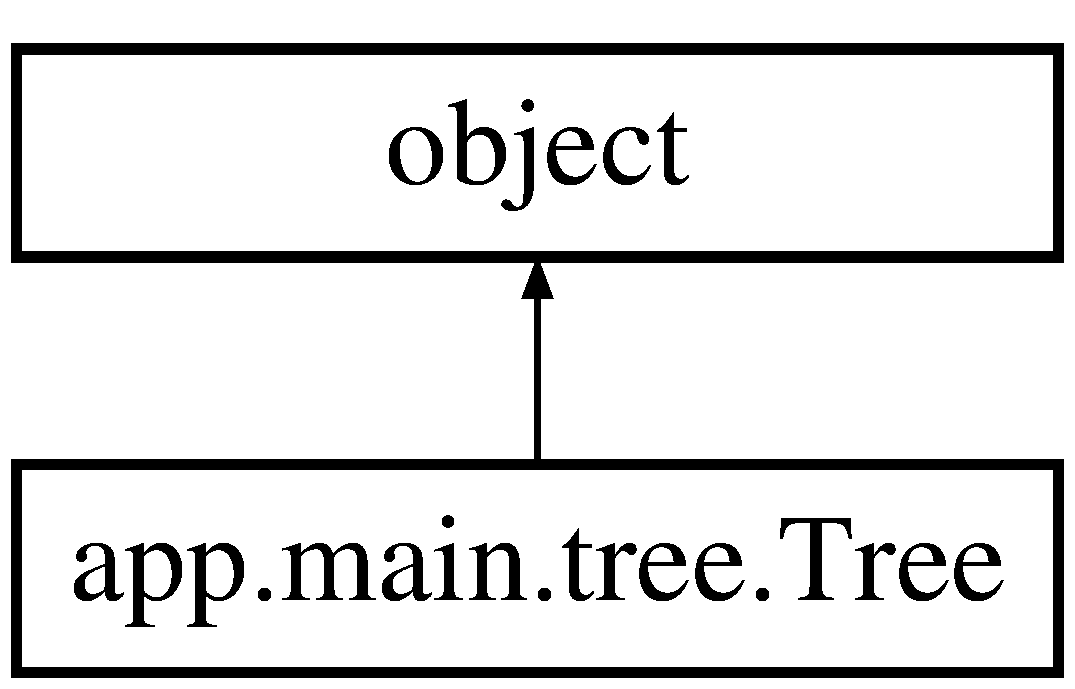
\includegraphics[height=2.000000cm]{classapp_1_1main_1_1tree_1_1Tree}
\end{center}
\end{figure}


The documentation for this class was generated from the following file\+:\begin{DoxyCompactItemize}
\item 
/home/nlarsson/bbk/python/webdev/museumflask/app/main/\mbox{\hyperlink{tree_8py}{tree.\+py}}\end{DoxyCompactItemize}

\hypertarget{classapp_1_1main_1_1datatypes_1_1Visitor__Numbers__Data_1_1Visitor__Numbers__Data}{}\section{app.\+main.\+datatypes.\+Visitor\+\_\+\+Numbers\+\_\+\+Data.\+Visitor\+\_\+\+Numbers\+\_\+\+Data Class Reference}
\label{classapp_1_1main_1_1datatypes_1_1Visitor__Numbers__Data_1_1Visitor__Numbers__Data}\index{app.\+main.\+datatypes.\+Visitor\+\_\+\+Numbers\+\_\+\+Data.\+Visitor\+\_\+\+Numbers\+\_\+\+Data@{app.\+main.\+datatypes.\+Visitor\+\_\+\+Numbers\+\_\+\+Data.\+Visitor\+\_\+\+Numbers\+\_\+\+Data}}
Inheritance diagram for app.\+main.\+datatypes.\+Visitor\+\_\+\+Numbers\+\_\+\+Data.\+Visitor\+\_\+\+Numbers\+\_\+\+Data\+:\begin{figure}[H]
\begin{center}
\leavevmode
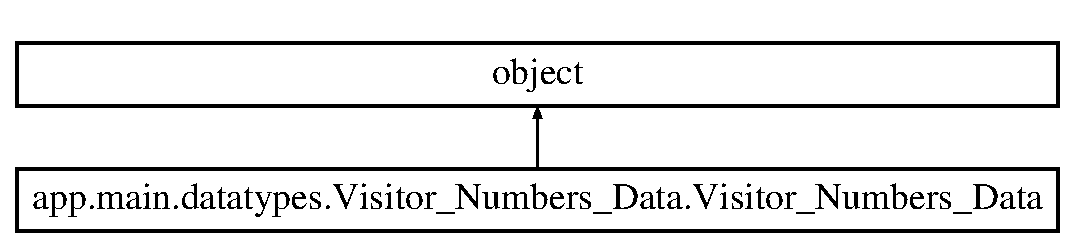
\includegraphics[height=2.000000cm]{classapp_1_1main_1_1datatypes_1_1Visitor__Numbers__Data_1_1Visitor__Numbers__Data}
\end{center}
\end{figure}
\subsection*{Public Member Functions}
\begin{DoxyCompactItemize}
\item 
\mbox{\Hypertarget{classapp_1_1main_1_1datatypes_1_1Visitor__Numbers__Data_1_1Visitor__Numbers__Data_a61f83caf0697e5de7e68edf700e38224}\label{classapp_1_1main_1_1datatypes_1_1Visitor__Numbers__Data_1_1Visitor__Numbers__Data_a61f83caf0697e5de7e68edf700e38224}} 
def {\bfseries \+\_\+\+\_\+init\+\_\+\+\_\+} (self)
\item 
\mbox{\Hypertarget{classapp_1_1main_1_1datatypes_1_1Visitor__Numbers__Data_1_1Visitor__Numbers__Data_a737460e6c29cf9448a38bbb0d2a5ece4}\label{classapp_1_1main_1_1datatypes_1_1Visitor__Numbers__Data_1_1Visitor__Numbers__Data_a737460e6c29cf9448a38bbb0d2a5ece4}} 
def {\bfseries get\+Match\+Filter} (self, rcount, match, condition)
\item 
\mbox{\Hypertarget{classapp_1_1main_1_1datatypes_1_1Visitor__Numbers__Data_1_1Visitor__Numbers__Data_a489e3ff90555ffec708190044009ff2c}\label{classapp_1_1main_1_1datatypes_1_1Visitor__Numbers__Data_1_1Visitor__Numbers__Data_a489e3ff90555ffec708190044009ff2c}} 
def {\bfseries get\+Compare\+Filter} (self, rcount, match, condition)
\item 
\mbox{\Hypertarget{classapp_1_1main_1_1datatypes_1_1Visitor__Numbers__Data_1_1Visitor__Numbers__Data_a39b48e0b80f75d8c5b973b96cfd16db4}\label{classapp_1_1main_1_1datatypes_1_1Visitor__Numbers__Data_1_1Visitor__Numbers__Data_a39b48e0b80f75d8c5b973b96cfd16db4}} 
def {\bfseries get\+Query} (self, col, rcount, matchstring, condition, matchcolumn)
\item 
\mbox{\Hypertarget{classapp_1_1main_1_1datatypes_1_1Visitor__Numbers__Data_1_1Visitor__Numbers__Data_a50778accf686b8a4fbdc148ea41b1458}\label{classapp_1_1main_1_1datatypes_1_1Visitor__Numbers__Data_1_1Visitor__Numbers__Data_a50778accf686b8a4fbdc148ea41b1458}} 
def {\bfseries get\+Search\+Type} (self)
\item 
\mbox{\Hypertarget{classapp_1_1main_1_1datatypes_1_1Visitor__Numbers__Data_1_1Visitor__Numbers__Data_a013920ead5fac6dfc160aafa9f4f9990}\label{classapp_1_1main_1_1datatypes_1_1Visitor__Numbers__Data_1_1Visitor__Numbers__Data_a013920ead5fac6dfc160aafa9f4f9990}} 
def {\bfseries get\+G\+U\+I\+Conditions} (self)
\item 
\mbox{\Hypertarget{classapp_1_1main_1_1datatypes_1_1Visitor__Numbers__Data_1_1Visitor__Numbers__Data_a9d0393ea3fe5a3d97cda76d28f77725a}\label{classapp_1_1main_1_1datatypes_1_1Visitor__Numbers__Data_1_1Visitor__Numbers__Data_a9d0393ea3fe5a3d97cda76d28f77725a}} 
def {\bfseries get\+Widget} (self)
\item 
\mbox{\Hypertarget{classapp_1_1main_1_1datatypes_1_1Visitor__Numbers__Data_1_1Visitor__Numbers__Data_aca77f987f32b1848166a88dd32a3bf3c}\label{classapp_1_1main_1_1datatypes_1_1Visitor__Numbers__Data_1_1Visitor__Numbers__Data_aca77f987f32b1848166a88dd32a3bf3c}} 
def {\bfseries get\+Widget\+Code} (self)
\item 
\mbox{\Hypertarget{classapp_1_1main_1_1datatypes_1_1Visitor__Numbers__Data_1_1Visitor__Numbers__Data_ac0ec7476fab84af5cc25f1214952d5cc}\label{classapp_1_1main_1_1datatypes_1_1Visitor__Numbers__Data_1_1Visitor__Numbers__Data_ac0ec7476fab84af5cc25f1214952d5cc}} 
def {\bfseries get\+Model\+To\+View\+O\+LD} (self, model)
\item 
\mbox{\Hypertarget{classapp_1_1main_1_1datatypes_1_1Visitor__Numbers__Data_1_1Visitor__Numbers__Data_a258f23d4503641d7a72f409c0fe1b0b0}\label{classapp_1_1main_1_1datatypes_1_1Visitor__Numbers__Data_1_1Visitor__Numbers__Data_a258f23d4503641d7a72f409c0fe1b0b0}} 
def {\bfseries get\+Model\+To\+View} (self, model, tup=None)
\item 
\mbox{\Hypertarget{classapp_1_1main_1_1datatypes_1_1Visitor__Numbers__Data_1_1Visitor__Numbers__Data_a8cd8dc1906638b47e614012ead6da39f}\label{classapp_1_1main_1_1datatypes_1_1Visitor__Numbers__Data_1_1Visitor__Numbers__Data_a8cd8dc1906638b47e614012ead6da39f}} 
def {\bfseries sort} (self, list)
\end{DoxyCompactItemize}
\subsection*{Static Public Attributes}
\begin{DoxyCompactItemize}
\item 
\mbox{\Hypertarget{classapp_1_1main_1_1datatypes_1_1Visitor__Numbers__Data_1_1Visitor__Numbers__Data_a29a66db90e04b19abb962698bd442f05}\label{classapp_1_1main_1_1datatypes_1_1Visitor__Numbers__Data_1_1Visitor__Numbers__Data_a29a66db90e04b19abb962698bd442f05}} 
{\bfseries query}
\item 
\mbox{\Hypertarget{classapp_1_1main_1_1datatypes_1_1Visitor__Numbers__Data_1_1Visitor__Numbers__Data_a9ce23a56096e2dfeeec9a3fdb1b2ae50}\label{classapp_1_1main_1_1datatypes_1_1Visitor__Numbers__Data_1_1Visitor__Numbers__Data_a9ce23a56096e2dfeeec9a3fdb1b2ae50}} 
{\bfseries parts} = model.\+split(\char`\"{}\+:\char`\"{})
\item 
\mbox{\Hypertarget{classapp_1_1main_1_1datatypes_1_1Visitor__Numbers__Data_1_1Visitor__Numbers__Data_a02ceaaa9c00473176d08058c9e09dace}\label{classapp_1_1main_1_1datatypes_1_1Visitor__Numbers__Data_1_1Visitor__Numbers__Data_a02ceaaa9c00473176d08058c9e09dace}} 
{\bfseries starty} = parts\mbox{[}2\mbox{]}
\item 
\mbox{\Hypertarget{classapp_1_1main_1_1datatypes_1_1Visitor__Numbers__Data_1_1Visitor__Numbers__Data_ad86cd985ad98e2dcd1c3c897c0baa0f9}\label{classapp_1_1main_1_1datatypes_1_1Visitor__Numbers__Data_1_1Visitor__Numbers__Data_ad86cd985ad98e2dcd1c3c897c0baa0f9}} 
{\bfseries vis} = parts\mbox{[}1\mbox{]}
\item 
string {\bfseries html}
\item 
\mbox{\Hypertarget{classapp_1_1main_1_1datatypes_1_1Visitor__Numbers__Data_1_1Visitor__Numbers__Data_aa3983dafcc6f2d006c848ff5b77bd4d5}\label{classapp_1_1main_1_1datatypes_1_1Visitor__Numbers__Data_1_1Visitor__Numbers__Data_aa3983dafcc6f2d006c848ff5b77bd4d5}} 
string {\bfseries view} = \char`\"{}\$\{visitors\} at \$\{from\}\char`\"{}
\item 
\mbox{\Hypertarget{classapp_1_1main_1_1datatypes_1_1Visitor__Numbers__Data_1_1Visitor__Numbers__Data_a10934f34e02ab4b3772f984dcad4f90a}\label{classapp_1_1main_1_1datatypes_1_1Visitor__Numbers__Data_1_1Visitor__Numbers__Data_a10934f34e02ab4b3772f984dcad4f90a}} 
{\bfseries tuplist} = None
\item 
\mbox{\Hypertarget{classapp_1_1main_1_1datatypes_1_1Visitor__Numbers__Data_1_1Visitor__Numbers__Data_a691ebc229996444216854c7aeaf17a6c}\label{classapp_1_1main_1_1datatypes_1_1Visitor__Numbers__Data_1_1Visitor__Numbers__Data_a691ebc229996444216854c7aeaf17a6c}} 
tuple {\bfseries tup} = (starty,vis)
\item 
\mbox{\Hypertarget{classapp_1_1main_1_1datatypes_1_1Visitor__Numbers__Data_1_1Visitor__Numbers__Data_adee3f34d15bf27b50eea2590aba904f2}\label{classapp_1_1main_1_1datatypes_1_1Visitor__Numbers__Data_1_1Visitor__Numbers__Data_adee3f34d15bf27b50eea2590aba904f2}} 
{\bfseries sortedlist} = sorted(tuplist,key=lambda tup\+: tup\mbox{[}0\mbox{]})
\item 
\mbox{\Hypertarget{classapp_1_1main_1_1datatypes_1_1Visitor__Numbers__Data_1_1Visitor__Numbers__Data_a530ff2fd43b9a00f6eecf60314359b97}\label{classapp_1_1main_1_1datatypes_1_1Visitor__Numbers__Data_1_1Visitor__Numbers__Data_a530ff2fd43b9a00f6eecf60314359b97}} 
list {\bfseries resultlist} = \mbox{[}$\,$\mbox{]}
\end{DoxyCompactItemize}


\subsection{Member Data Documentation}
\mbox{\Hypertarget{classapp_1_1main_1_1datatypes_1_1Visitor__Numbers__Data_1_1Visitor__Numbers__Data_ae13967a136e51f26a473c7b50ab13c47}\label{classapp_1_1main_1_1datatypes_1_1Visitor__Numbers__Data_1_1Visitor__Numbers__Data_ae13967a136e51f26a473c7b50ab13c47}} 
\index{app\+::main\+::datatypes\+::\+Visitor\+\_\+\+Numbers\+\_\+\+Data\+::\+Visitor\+\_\+\+Numbers\+\_\+\+Data@{app\+::main\+::datatypes\+::\+Visitor\+\_\+\+Numbers\+\_\+\+Data\+::\+Visitor\+\_\+\+Numbers\+\_\+\+Data}!html@{html}}
\index{html@{html}!app\+::main\+::datatypes\+::\+Visitor\+\_\+\+Numbers\+\_\+\+Data\+::\+Visitor\+\_\+\+Numbers\+\_\+\+Data@{app\+::main\+::datatypes\+::\+Visitor\+\_\+\+Numbers\+\_\+\+Data\+::\+Visitor\+\_\+\+Numbers\+\_\+\+Data}}
\subsubsection{\texorpdfstring{html}{html}}
{\footnotesize\ttfamily string app.\+main.\+datatypes.\+Visitor\+\_\+\+Numbers\+\_\+\+Data.\+Visitor\+\_\+\+Numbers\+\_\+\+Data.\+html\hspace{0.3cm}{\ttfamily [static]}}

{\bfseries Initial value\+:}
\begin{DoxyCode}{0}
\DoxyCodeLine{= \textcolor{stringliteral}{"""}}
\DoxyCodeLine{\textcolor{stringliteral}{       <table id="visitornumbersdata"  class="table table-bordered" border="1"  >}}
\DoxyCodeLine{\textcolor{stringliteral}{   <thead>}}
\DoxyCodeLine{\textcolor{stringliteral}{       <tr>}}
\DoxyCodeLine{\textcolor{stringliteral}{               <th id="vn-heading1" > }}
\DoxyCodeLine{\textcolor{stringliteral}{                   Num}}
\DoxyCodeLine{\textcolor{stringliteral}{                </th>}}
\DoxyCodeLine{\textcolor{stringliteral}{               <th id="vn-heading2" > }}
\DoxyCodeLine{\textcolor{stringliteral}{                   At}}
\DoxyCodeLine{\textcolor{stringliteral}{                </th>}}
\DoxyCodeLine{\textcolor{stringliteral}{       </tr>}}
\DoxyCodeLine{\textcolor{stringliteral}{   </thead>}}
\DoxyCodeLine{\textcolor{stringliteral}{<tbody>}}
\DoxyCodeLine{\textcolor{stringliteral}{      <tr  class="vnresult">}}
\DoxyCodeLine{\textcolor{stringliteral}{             <td  class="vn-status"> \$\{visitors\} </td>}}
\DoxyCodeLine{\textcolor{stringliteral}{             <td  class="vn-from">   \$\{from\} </td>}}
\DoxyCodeLine{\textcolor{stringliteral}{          </tr>}}
\DoxyCodeLine{\textcolor{stringliteral}{</tbody>}}
\DoxyCodeLine{\textcolor{stringliteral}{       </table>}}
\DoxyCodeLine{\textcolor{stringliteral}{}}
\DoxyCodeLine{\textcolor{stringliteral}{}}
\DoxyCodeLine{\textcolor{stringliteral}{"""}}
\end{DoxyCode}


The documentation for this class was generated from the following file\+:\begin{DoxyCompactItemize}
\item 
/home/nlarsson/bbk/python/webdev/museumflask/app/main/datatypes/\mbox{\hyperlink{Visitor__Numbers__Data_8py}{Visitor\+\_\+\+Numbers\+\_\+\+Data.\+py}}\end{DoxyCompactItemize}

\chapter{File Documentation}
\hypertarget{admingeoservice_8py}{}\section{/home/nlarsson/bbk/python/webdev/museumflask/app/main/admingeoservice.py File Reference}
\label{admingeoservice_8py}\index{/home/nlarsson/bbk/python/webdev/museumflask/app/main/admingeoservice.\+py@{/home/nlarsson/bbk/python/webdev/museumflask/app/main/admingeoservice.\+py}}


~\newline
 This is an A\+PI service for the search front end to provide locations from the geo graph that matches the users characters as they type.  


\subsection*{Classes}
\begin{DoxyCompactItemize}
\item 
class \mbox{\hyperlink{classapp_1_1main_1_1admingeoservice_1_1Admingeoservice}{app.\+main.\+admingeoservice.\+Admingeoservice}}
\end{DoxyCompactItemize}
\subsection*{Functions}
\begin{DoxyCompactItemize}
\item 
\mbox{\Hypertarget{admingeoservice_8py_a8b7e130054af37d76d0f7c50318ce881}\label{admingeoservice_8py_a8b7e130054af37d76d0f7c50318ce881}} 
def \mbox{\hyperlink{admingeoservice_8py_a8b7e130054af37d76d0f7c50318ce881}{app.\+main.\+admingeoservice.\+get}} (self, propertytodisplay)
\begin{DoxyCompactList}\small\item\em Purpose\+: Returns a set of geonames matching the propertytodisplay parameters starting letters Arguments\+:  The starting letters to match. \end{DoxyCompactList}\end{DoxyCompactItemize}
\subsection*{Variables}
\begin{DoxyCompactItemize}
\item 
\mbox{\Hypertarget{admingeoservice_8py_a9997c1609fb6a16fdfb83e1222b0594d}\label{admingeoservice_8py_a9997c1609fb6a16fdfb83e1222b0594d}} 
{\bfseries app.\+main.\+admingeoservice.\+lcaseprop}
\item 
\mbox{\Hypertarget{admingeoservice_8py_ae1a79fbf6019f5cf8dc675ccde110a96}\label{admingeoservice_8py_ae1a79fbf6019f5cf8dc675ccde110a96}} 
{\bfseries app.\+main.\+admingeoservice.\+sparql} = S\+P\+A\+R\+Q\+L\+Wrapper(app.\+config\mbox{[}\textquotesingle{}S\+P\+A\+R\+Q\+L\+E\+N\+D\+P\+O\+I\+NT\textquotesingle{}\mbox{]})
\item 
string {\bfseries app.\+main.\+admingeoservice.\+queryold}
\item 
string {\bfseries app.\+main.\+admingeoservice.\+query}
\item 
\mbox{\Hypertarget{admingeoservice_8py_aef27d58570b11a682c4a34239f1ac8b2}\label{admingeoservice_8py_aef27d58570b11a682c4a34239f1ac8b2}} 
string {\bfseries app.\+main.\+admingeoservice.\+results} = sparql.\+query().convert()
\item 
\mbox{\Hypertarget{admingeoservice_8py_aed3c814758068b94f24197115c68ff03}\label{admingeoservice_8py_aed3c814758068b94f24197115c68ff03}} 
list {\bfseries app.\+main.\+admingeoservice.\+proplist} = \mbox{[}$\,$\mbox{]}
\item 
\mbox{\Hypertarget{admingeoservice_8py_a606e16329aab0f8034b66c2a2db05c68}\label{admingeoservice_8py_a606e16329aab0f8034b66c2a2db05c68}} 
string {\bfseries app.\+main.\+admingeoservice.\+vars} = results\mbox{[}\textquotesingle{}head\textquotesingle{}\mbox{]}\mbox{[}\textquotesingle{}vars\textquotesingle{}\mbox{]}
\item 
\mbox{\Hypertarget{admingeoservice_8py_ad121d7ff0d1219866c69c3f4bfeccba6}\label{admingeoservice_8py_ad121d7ff0d1219866c69c3f4bfeccba6}} 
{\bfseries app.\+main.\+admingeoservice.\+ps} = set(proplist)
\end{DoxyCompactItemize}


\subsection{Detailed Description}
~\newline
 This is an A\+PI service for the search front end to provide locations from the geo graph that matches the users characters as they type. 

~\newline
 More details. \$\$\+Author\$\+:Nick Larsson, Researcher, Dep. of Computer Science and Information Systems at Birkbeck University, London, England, email\+:\href{mailto:nick@dcs.bbk.ac.uk}{\tt nick@dcs.\+bbk.\+ac.\+uk}, License\+:G\+NU G\+P\+Lv3 

\subsection{Variable Documentation}
\mbox{\Hypertarget{admingeoservice_8py_aa89f48da918b1158eeb18a5b38f21f73}\label{admingeoservice_8py_aa89f48da918b1158eeb18a5b38f21f73}} 
\index{admingeoservice.\+py@{admingeoservice.\+py}!query@{query}}
\index{query@{query}!admingeoservice.\+py@{admingeoservice.\+py}}
\subsubsection{\texorpdfstring{query}{query}}
{\footnotesize\ttfamily string app.\+main.\+admingeoservice.\+query}

{\bfseries Initial value\+:}
\begin{DoxyCode}{0}
\DoxyCodeLine{1 = definitions.RDF\_PREFIX\_PRELUDE+\textcolor{stringliteral}{"""}}
\DoxyCodeLine{2 \textcolor{stringliteral}{    prefix """}+definitions.PREFIX\_WITHCOLON+\textcolor{stringliteral}{""" <http://"""}+definitions.RDFDEFURI+\textcolor{stringliteral}{"""> }}
\DoxyCodeLine{3 \textcolor{stringliteral}{    }}
\DoxyCodeLine{4 \textcolor{stringliteral}{}}
\DoxyCodeLine{5 \textcolor{stringliteral}{}}
\DoxyCodeLine{6 \textcolor{stringliteral}{}}
\DoxyCodeLine{7 \textcolor{stringliteral}{    SELECT DISTINCT STR(?sname) }}
\DoxyCodeLine{8 \textcolor{stringliteral}{    FROM <"""}+app.config[\textcolor{stringliteral}{'GEOADMINGRAPH'}]+\textcolor{stringliteral}{""">}}
\DoxyCodeLine{9 \textcolor{stringliteral}{    WHERE \{ }}
\DoxyCodeLine{10 \textcolor{stringliteral}{    ?adm bbkmm:hasTypedName  ?sname .}}
\DoxyCodeLine{11 \textcolor{stringliteral}{    ?adm a ?clazz .}}
\DoxyCodeLine{12 \textcolor{stringliteral}{    }}
\DoxyCodeLine{13 \textcolor{stringliteral}{    FILTER(STRSTARTS( LCASE(?sname),"""}+\textcolor{stringliteral}{'"'}+lcaseprop+\textcolor{stringliteral}{'"'}+\textcolor{stringliteral}{""")) }}
\DoxyCodeLine{14 \textcolor{stringliteral}{}}
\DoxyCodeLine{15 \textcolor{stringliteral}{}}
\DoxyCodeLine{16 \textcolor{stringliteral}{    \}}}
\DoxyCodeLine{17 \textcolor{stringliteral}{    group by ?sname order by ?sname}}
\DoxyCodeLine{18 \textcolor{stringliteral}{              }}
\DoxyCodeLine{19 \textcolor{stringliteral}{        """}}
\end{DoxyCode}
\mbox{\Hypertarget{admingeoservice_8py_a03bda54808931cf598782a9d968c67ea}\label{admingeoservice_8py_a03bda54808931cf598782a9d968c67ea}} 
\index{admingeoservice.\+py@{admingeoservice.\+py}!queryold@{queryold}}
\index{queryold@{queryold}!admingeoservice.\+py@{admingeoservice.\+py}}
\subsubsection{\texorpdfstring{queryold}{queryold}}
{\footnotesize\ttfamily string app.\+main.\+admingeoservice.\+queryold}

{\bfseries Initial value\+:}
\begin{DoxyCode}{0}
\DoxyCodeLine{1 = definitions.RDF\_PREFIX\_PRELUDE+\textcolor{stringliteral}{"""}}
\DoxyCodeLine{2 \textcolor{stringliteral}{    prefix """}+definitions.PREFIX\_WITHCOLON+\textcolor{stringliteral}{""" <http://"""}+definitions.RDFDEFURI+\textcolor{stringliteral}{"""> }}
\DoxyCodeLine{3 \textcolor{stringliteral}{    }}
\DoxyCodeLine{4 \textcolor{stringliteral}{    SELECT DISTINCT  Str(?subname)  Str(?ssname) Str(?sssname) }}
\DoxyCodeLine{5 \textcolor{stringliteral}{    FROM <"""}+app.config[\textcolor{stringliteral}{'GEOADMINGRAPH'}]+\textcolor{stringliteral}{""">}}
\DoxyCodeLine{6 \textcolor{stringliteral}{}}
\DoxyCodeLine{7 \textcolor{stringliteral}{}}
\DoxyCodeLine{8 \textcolor{stringliteral}{    WHERE \{ }}
\DoxyCodeLine{9 \textcolor{stringliteral}{    ?adm a bbkmm:Country .}}
\DoxyCodeLine{10 \textcolor{stringliteral}{    OPTIONAL\{}}
\DoxyCodeLine{11 \textcolor{stringliteral}{    ?adm bbkmm:contains ?sub .}}
\DoxyCodeLine{12 \textcolor{stringliteral}{    ?sub  bbkmm:hasTypedName  ?subname .}}
\DoxyCodeLine{13 \textcolor{stringliteral}{    FILTER(STRSTARTS( LCASE(?subname),"""}+\textcolor{stringliteral}{'"'}+lcaseprop+\textcolor{stringliteral}{'"'}+\textcolor{stringliteral}{""")) }}
\DoxyCodeLine{14 \textcolor{stringliteral}{    }}
\DoxyCodeLine{15 \textcolor{stringliteral}{    \}}}
\DoxyCodeLine{16 \textcolor{stringliteral}{    OPTIONAL\{}}
\DoxyCodeLine{17 \textcolor{stringliteral}{    ?sub bbkmm:contains ?subsub .}}
\DoxyCodeLine{18 \textcolor{stringliteral}{    ?subsub bbkmm:hasTypedName ?ssname .}}
\DoxyCodeLine{19 \textcolor{stringliteral}{    FILTER (STRSTARTS( LCASE(?ssname),"""}+\textcolor{stringliteral}{'"'}+lcaseprop+\textcolor{stringliteral}{'"'}+\textcolor{stringliteral}{""")) }}
\DoxyCodeLine{20 \textcolor{stringliteral}{    \}}}
\DoxyCodeLine{21 \textcolor{stringliteral}{    OPTIONAL \{}}
\DoxyCodeLine{22 \textcolor{stringliteral}{    ?subsub bbkmm:contains ?subsubsub .}}
\DoxyCodeLine{23 \textcolor{stringliteral}{    ?subsubsub bbkmm:hasTypedName ?sssname}}
\DoxyCodeLine{24 \textcolor{stringliteral}{    FILTER (STRSTARTS( LCASE(?sssname),"""}+\textcolor{stringliteral}{'"'}+lcaseprop+\textcolor{stringliteral}{'"'}+\textcolor{stringliteral}{""")) }}
\DoxyCodeLine{25 \textcolor{stringliteral}{    \}}}
\DoxyCodeLine{26 \textcolor{stringliteral}{    \}group by ?subname order by ?subname}}
\DoxyCodeLine{27 \textcolor{stringliteral}{              }}
\DoxyCodeLine{28 \textcolor{stringliteral}{        """}}
\end{DoxyCode}

\hypertarget{apputils_8py}{}\section{/home/nlarsson/bbk/python/webdev/museumflask/app/main/apputils.py File Reference}
\label{apputils_8py}\index{/home/nlarsson/bbk/python/webdev/museumflask/app/main/apputils.\+py@{/home/nlarsson/bbk/python/webdev/museumflask/app/main/apputils.\+py}}


This module implements \+: 1.  


\subsection*{Functions}
\begin{DoxyCompactItemize}
\item 
\mbox{\Hypertarget{apputils_8py_a965ccb2fb5539f85fd30953516f34153}\label{apputils_8py_a965ccb2fb5539f85fd30953516f34153}} 
def \mbox{\hyperlink{apputils_8py_a965ccb2fb5539f85fd30953516f34153}{app.\+main.\+apputils.\+rotate}} (l, n)
\begin{DoxyCompactList}\small\item\em Purpose\+:Small set of functions to change the appearance of names (strings) \end{DoxyCompactList}\item 
\mbox{\Hypertarget{apputils_8py_a6bfeb06651b70211f731c00b43d541b0}\label{apputils_8py_a6bfeb06651b70211f731c00b43d541b0}} 
def {\bfseries app.\+main.\+apputils.\+snake2camel} (name)
\item 
\mbox{\Hypertarget{apputils_8py_ada4afaa18d754f234165ae5d291feb15}\label{apputils_8py_ada4afaa18d754f234165ae5d291feb15}} 
def {\bfseries app.\+main.\+apputils.\+snake2camelback} (name)
\item 
\mbox{\Hypertarget{apputils_8py_a551acda6763aa89c807cf96042acf4b4}\label{apputils_8py_a551acda6763aa89c807cf96042acf4b4}} 
def {\bfseries app.\+main.\+apputils.\+camel2snake} (name)
\item 
\mbox{\Hypertarget{apputils_8py_a1112ebc12b6fff5f7a85d8e0cad48b27}\label{apputils_8py_a1112ebc12b6fff5f7a85d8e0cad48b27}} 
def {\bfseries app.\+main.\+apputils.\+camelback2snake} (name)
\item 
\mbox{\Hypertarget{apputils_8py_a51b9b90e79e7177f87d2bb4bc32504ba}\label{apputils_8py_a51b9b90e79e7177f87d2bb4bc32504ba}} 
def \mbox{\hyperlink{apputils_8py_a51b9b90e79e7177f87d2bb4bc32504ba}{app.\+main.\+apputils.\+read\+O\+N\+S\+P\+C\+Repo}} (fname, lafname, postcode2\+\_\+county\+\_\+dict, postcode2\+\_\+country\+\_\+dict, postcode2\+\_\+la\+\_\+dict, postcode2\+\_\+region\+\_\+dict, county2\+\_\+region\+\_\+dict, la2\+\_\+county\+\_\+dict, la2\+\_\+region\+\_\+dict, la\+\_\+translation\+\_\+dict, reverse\+\_\+la\+\_\+translation\+\_\+dict)
\begin{DoxyCompactList}\small\item\em Purpose\+: Reads the O\+NS csv data creates all dictionaries needed for processing Arguments\+:  name of ons file  local authority definition file         . \end{DoxyCompactList}\item 
def \mbox{\hyperlink{apputils_8py_a26d1beaec54c0632a0b603a8bb1a9ba9}{app.\+main.\+apputils.\+read\+Names}} (fname)
\begin{DoxyCompactList}\small\item\em Purpose\+: Reads district and county names. \end{DoxyCompactList}\item 
\mbox{\Hypertarget{apputils_8py_a72c2a9fc4b8c4b0b21c5c2c358eb5b3e}\label{apputils_8py_a72c2a9fc4b8c4b0b21c5c2c358eb5b3e}} 
def \mbox{\hyperlink{apputils_8py_a72c2a9fc4b8c4b0b21c5c2c358eb5b3e}{app.\+main.\+apputils.\+read\+Admin\+Data}} ()
\begin{DoxyCompactList}\small\item\em Purpose\+:Sets up reading of the O\+NS data Arguments\+: \end{DoxyCompactList}\item 
def \mbox{\hyperlink{apputils_8py_a4b57a30a8b9a67d46b6b0bbd37d365a5}{app.\+main.\+apputils.\+read\+List}} (fname)
\begin{DoxyCompactList}\small\item\em Purpose\+:Reads a list of names from a file. \end{DoxyCompactList}\item 
def \mbox{\hyperlink{apputils_8py_a6f4ac21e7ea329c188677915a341ddbc}{app.\+main.\+apputils.\+create\+Reset\+Lists}} (listnames)
\begin{DoxyCompactList}\small\item\em Purpose\+:Creates an R\+DF list of values for properties in listnames. \end{DoxyCompactList}\item 
def \mbox{\hyperlink{apputils_8py_aac45e0b43fbc295d84ea2c8e3003f600}{app.\+main.\+apputils.\+get\+Values\+For\+Type}} (colname, typename)
\begin{DoxyCompactList}\small\item\em Purpose\+:Generates a unique list of values for a property from the DB Arguments\+: \end{DoxyCompactList}\item 
def \mbox{\hyperlink{apputils_8py_a1689e1921c890b50b1daf2233e1527fa}{app.\+main.\+apputils.\+create\+List\+Of\+All\+Values}} (colname, typename, attritypes)
\begin{DoxyCompactList}\small\item\em Purpose\+: Generates a unique list of values for a column from a map and inserts it in db Arguments\+: \end{DoxyCompactList}\item 
def \mbox{\hyperlink{apputils_8py_a4a11e02db98c8471b91d4167dd395c29}{app.\+main.\+apputils.\+create\+List\+Cache}} (listnames)
\begin{DoxyCompactList}\small\item\em Purpose\+:\# Creates a cache for all lists accessibel by name key Called in models ini Arguments\+: \end{DoxyCompactList}\item 
\mbox{\Hypertarget{apputils_8py_a809cbfd3a60e2b1de72389c4cf1fd9b3}\label{apputils_8py_a809cbfd3a60e2b1de72389c4cf1fd9b3}} 
def {\bfseries app.\+main.\+apputils.\+getall\+Museums\+Of\+Property} (property)
\item 
def \mbox{\hyperlink{apputils_8py_a1e9d585f9bd50aaaf11ba5d8a0e201fa}{app.\+main.\+apputils.\+get\+Museum\+Properties\+For\+Id}} (shortid)
\begin{DoxyCompactList}\small\item\em Purpose\+:Get all properties for a museum with id Arguments\+: \end{DoxyCompactList}\item 
def \mbox{\hyperlink{apputils_8py_aad1c9685bb71266d6e0ed705524e6a44}{app.\+main.\+apputils.\+get\+Viz\+Location\+Data}} (patharray, startperiod, endperiod, columns=None, locationname=\char`\"{}location\char`\"{})
\begin{DoxyCompactList}\small\item\em Purpose\+:Get data for use with the Admin data property of O\+NS classifications for visualisation Arguments\+: \end{DoxyCompactList}\item 
def \mbox{\hyperlink{apputils_8py_afe0daadd8f0f852049828b0c9fc6d92c}{app.\+main.\+apputils.\+get\+Marker\+Data}} (columns, filters=None, vardict=None)
\begin{DoxyCompactList}\small\item\em Purpose\+:Retrieves data to be used with the browse page Arguments\+: \end{DoxyCompactList}\item 
def \mbox{\hyperlink{apputils_8py_a44a09238ce2bbb0a2e2c047e39d296f4}{app.\+main.\+apputils.\+get\+Museum\+Properties\+For\+Id\+Working}} (shortid)
\begin{DoxyCompactList}\small\item\em Purpose\+:Removes type info from name Arguments\+: \end{DoxyCompactList}\item 
def \mbox{\hyperlink{apputils_8py_a25aa0b31ab1007f23970be3a583e3ce7}{app.\+main.\+apputils.\+is\+Data\+Class}} (clazz)
\begin{DoxyCompactList}\small\item\em Purpose\+:Is this clazz an abstract clazz? Obviously the hard coding needs to go. \end{DoxyCompactList}\item 
def \mbox{\hyperlink{apputils_8py_ae149d9fda553dbf30db32b8d431f81a6}{app.\+main.\+apputils.\+get\+Data\+Class\+Instance}} (clazz)
\begin{DoxyCompactList}\small\item\em Purpose\+:Loads a class inmplementation Arguments\+: \end{DoxyCompactList}\item 
def \mbox{\hyperlink{apputils_8py_a7dd7e769be80ca45afe9e52dfd5df0dc}{app.\+main.\+apputils.\+discover\+Datatypes}} (datadict)
\begin{DoxyCompactList}\small\item\em Purpose\+:Look for data type implementations and create a cache This works both on the attritypes (L\+I\+ST) and the datadict (D\+I\+CT) so we need to check which it is Arguments\+: \end{DoxyCompactList}\item 
def \mbox{\hyperlink{apputils_8py_adb609a6b67aa6c22551e87c1deb621b6}{app.\+main.\+apputils.\+getdatagroups}} (attributetypes)
\begin{DoxyCompactList}\small\item\em Purpose\+:Creates the select menu for the datatypes used in search loop over all types picking non xml datatype add List to typename (dataproperty) get list from database add all elements of list as group\+:typename to map Arguments\+: \end{DoxyCompactList}\item 
def \mbox{\hyperlink{apputils_8py_a5e9522aa08c916a54a117070b1052362}{app.\+main.\+apputils.\+getpredicatestypes}} ()
\begin{DoxyCompactList}\small\item\em Purpose\+:Retrieves classes and predicates. \end{DoxyCompactList}\item 
\mbox{\Hypertarget{apputils_8py_a94bd572b5647553a38e29c43c1dbcf5e}\label{apputils_8py_a94bd572b5647553a38e29c43c1dbcf5e}} 
def \mbox{\hyperlink{apputils_8py_a94bd572b5647553a38e29c43c1dbcf5e}{app.\+main.\+apputils.\+getmuseumpredicates}} ()
\begin{DoxyCompactList}\small\item\em Purpose\+:Retrieves all predicats relating to a museum. \end{DoxyCompactList}\item 
def \mbox{\hyperlink{apputils_8py_a00681d09a94f5f4c0311e7b8ba627d50}{app.\+main.\+apputils.\+get\+Defined\+Type}} (incol)
\begin{DoxyCompactList}\small\item\em Purpose\+:Returns the column if defined in the datatyep map Arguments\+: \end{DoxyCompactList}\item 
def \mbox{\hyperlink{apputils_8py_a830894546b2b8fa295df421b5e77b866}{app.\+main.\+apputils.\+is\+Type\+A\+Clazz}} (incol, defcol)
\begin{DoxyCompactList}\small\item\em Purpose\+:Is this column an abstract type? Arguments\+: \end{DoxyCompactList}\item 
def \mbox{\hyperlink{apputils_8py_a0873bf11568456a2cef3dc293b4983a3}{app.\+main.\+apputils.\+get\+Query\+For\+Col}} (incol, rcount, optional=True, museumuri=\textquotesingle{}?museum \textquotesingle{}, matchstrings=\mbox{[}$\,$\mbox{]}, conditions=\mbox{[}$\,$\mbox{]}, matchcolumns=\mbox{[}$\,$\mbox{]}, coltoargdict=\{\})
\begin{DoxyCompactList}\small\item\em Purpose\+:Creates a query for a column Arguments\+: \end{DoxyCompactList}\item 
def \mbox{\hyperlink{apputils_8py_a66fda77a1920dc5eae535a18391c63f5}{app.\+main.\+apputils.\+get\+Col}} (col, coltocountdict, lowerorupper=\char`\"{}\char`\"{})
\begin{DoxyCompactList}\small\item\em Purpose\+:Create virtuoso data type statement for column Arguments\+: \end{DoxyCompactList}\item 
def \mbox{\hyperlink{apputils_8py_afdb0219b81b60073e446bf8a0dd5018e}{app.\+main.\+apputils.\+get\+Filter\+Clause}} (matchcolumns, conditions, matchstrings, coltocountdict)
\begin{DoxyCompactList}\small\item\em Purpose\+:Returns a filter clause for a column Arguments\+: \end{DoxyCompactList}\item 
def \mbox{\hyperlink{apputils_8py_a03446e0814a13147c1dfa0446969ba58}{app.\+main.\+apputils.\+get\+Search\+Results}} (columns, matchcolumns, conditions, matchstrings, ordercolumn)
\begin{DoxyCompactList}\small\item\em Purpose\+:Create a query for a list of columns Arguments\+: \end{DoxyCompactList}\end{DoxyCompactItemize}
\subsection*{Variables}
\begin{DoxyCompactItemize}
\item 
dictionary {\bfseries app.\+main.\+apputils.\+R\+E\+V\+E\+R\+S\+E\+\_\+\+C\+O\+U\+N\+T\+R\+Y\+\_\+\+T\+R\+A\+N\+S\+L\+A\+T\+I\+O\+N\+\_\+\+T\+A\+B\+LE}
\item 
dictionary {\bfseries app.\+main.\+apputils.\+C\+O\+U\+N\+T\+R\+Y\+\_\+\+T\+R\+A\+N\+S\+L\+A\+T\+I\+O\+N\+\_\+\+T\+A\+B\+LE}
\item 
\mbox{\Hypertarget{apputils_8py_aca78671a184a45c163d4bdf257f21777}\label{apputils_8py_aca78671a184a45c163d4bdf257f21777}} 
dictionary {\bfseries app.\+main.\+apputils.\+C\+O\+U\+N\+T\+Y\+\_\+\+T\+R\+A\+N\+S\+L\+A\+T\+I\+O\+N\+\_\+\+T\+A\+B\+LE}
\item 
\mbox{\Hypertarget{apputils_8py_af56153938c9589e68f0b2f609cd801c1}\label{apputils_8py_af56153938c9589e68f0b2f609cd801c1}} 
dictionary {\bfseries app.\+main.\+apputils.\+R\+E\+V\+E\+R\+S\+E\+\_\+\+C\+O\+U\+N\+T\+Y\+\_\+\+T\+R\+A\+N\+S\+L\+A\+T\+I\+O\+N\+\_\+\+T\+A\+B\+LE}
\item 
dictionary {\bfseries app.\+main.\+apputils.\+G\+O\+R\+\_\+\+T\+R\+A\+N\+S\+L\+A\+T\+I\+O\+N\+\_\+\+T\+A\+B\+LE}
\item 
dictionary {\bfseries app.\+main.\+apputils.\+R\+E\+V\+E\+R\+S\+E\+\_\+\+G\+O\+R\+\_\+\+T\+R\+A\+N\+S\+L\+A\+T\+I\+O\+N\+\_\+\+T\+A\+B\+LE}
\item 
dictionary {\bfseries app.\+main.\+apputils.\+C\+A\+\_\+\+C\+O\+D\+E\+\_\+\+T\+O\+\_\+\+G\+O\+R\+\_\+\+T\+A\+B\+LE}
\item 
dictionary {\bfseries app.\+main.\+apputils.\+C\+A\+\_\+\+C\+O\+D\+E\+\_\+\+T\+O\+\_\+\+N\+A\+M\+E\+\_\+\+T\+A\+B\+LE}
\item 
dictionary {\bfseries app.\+main.\+apputils.\+R\+E\+V\+E\+R\+S\+E\+\_\+\+C\+A\+\_\+\+C\+O\+D\+E\+\_\+\+T\+O\+\_\+\+N\+A\+M\+E\+\_\+\+T\+A\+B\+LE}
\item 
\mbox{\Hypertarget{apputils_8py_acf32b3f153712ec7736b2d16d5a20d22}\label{apputils_8py_acf32b3f153712ec7736b2d16d5a20d22}} 
dictionary {\bfseries app.\+main.\+apputils.\+L\+A\+\_\+\+T\+O\+\_\+\+C\+A\+\_\+\+C\+O\+D\+E\+S\+\_\+\+T\+A\+B\+LE}
\item 
\mbox{\Hypertarget{apputils_8py_ac1264553a66f6edae499625a830095fd}\label{apputils_8py_ac1264553a66f6edae499625a830095fd}} 
dictionary {\bfseries app.\+main.\+apputils.\+L\+A\+\_\+\+T\+O\+\_\+\+C\+A\+\_\+\+N\+A\+M\+E\+S\+\_\+\+T\+A\+B\+LE}
\item 
\mbox{\Hypertarget{apputils_8py_ad2849efa36bf2f32795de19b10d82289}\label{apputils_8py_ad2849efa36bf2f32795de19b10d82289}} 
dictionary {\bfseries app.\+main.\+apputils.\+L\+A\+\_\+\+T\+R\+A\+N\+S\+L\+A\+T\+I\+O\+N\+\_\+\+T\+A\+B\+LE} = \{\}
\item 
\mbox{\Hypertarget{apputils_8py_a0f8f2c775f4b1e8cd185164541799a52}\label{apputils_8py_a0f8f2c775f4b1e8cd185164541799a52}} 
dictionary {\bfseries app.\+main.\+apputils.\+R\+E\+V\+E\+R\+S\+E\+\_\+\+L\+A\+\_\+\+T\+R\+A\+N\+S\+L\+A\+T\+I\+O\+N\+\_\+\+T\+A\+B\+LE} = \{\}
\item 
\mbox{\Hypertarget{apputils_8py_aa315f623fd020c499508e6cf2b777cdd}\label{apputils_8py_aa315f623fd020c499508e6cf2b777cdd}} 
{\bfseries app.\+main.\+apputils.\+modeltoview} = model\+\_\+to\+\_\+view.\+Model\+\_\+\+To\+\_\+\+View()
\item 
\mbox{\hyperlink{apputils_8py_a69d63b46b6b7c27fe1df03e37bdbbc13}{app.\+main.\+apputils.\+vizgeoquery}} = vizgeoquery.\+replace(key.\+strip(),val.\+strip())
\begin{DoxyCompactList}\small\item\em Deal with the visualisation geo query Once this works it should be turned into a ligthweight datatype class that can be added dynamically and does not have all the search interfaces. \end{DoxyCompactList}\item 
\mbox{\Hypertarget{apputils_8py_a4dffa204a19eb28ce6b63b36fdd9d644}\label{apputils_8py_a4dffa204a19eb28ce6b63b36fdd9d644}} 
{\bfseries app.\+main.\+apputils.\+geoquery} = vizgeoquery
\item 
\mbox{\Hypertarget{apputils_8py_a59100073c2155431943fe6f89df06a3f}\label{apputils_8py_a59100073c2155431943fe6f89df06a3f}} 
string {\bfseries app.\+main.\+apputils.\+queryparams} = queryparams+\char`\"{}?\char`\"{}+definitions.\+G\+E\+O\+C\+OL+\char`\"{} \char`\"{}
\item 
\mbox{\Hypertarget{apputils_8py_af65c36a426ea9d4f5507e389285e2ab8}\label{apputils_8py_af65c36a426ea9d4f5507e389285e2ab8}} 
{\bfseries app.\+main.\+apputils.\+vizadmgeoquery} = vizadmgeoquery.\+replace(key.\+strip(),val.\+strip())
\item 
\mbox{\Hypertarget{apputils_8py_a888d2381d7415db1c737c314d9930313}\label{apputils_8py_a888d2381d7415db1c737c314d9930313}} 
string {\bfseries app.\+main.\+apputils.\+filter} = filter+f+\char`\"{} . \textbackslash{}n\char`\"{}
\item 
\mbox{\Hypertarget{apputils_8py_a22cb223de832e5d9d70271bae44c4de6}\label{apputils_8py_a22cb223de832e5d9d70271bae44c4de6}} 
int {\bfseries app.\+main.\+apputils.\+rcount} = 1
\item 
\mbox{\Hypertarget{apputils_8py_ac20d0fc2c283d6e4997c58e964c90830}\label{apputils_8py_ac20d0fc2c283d6e4997c58e964c90830}} 
{\bfseries app.\+main.\+apputils.\+querycols} = querycols+get\+Query\+For\+Col(col,rcount)
\item 
\mbox{\Hypertarget{apputils_8py_a32827ce26d3309cdbda06fe1bc91d4aa}\label{apputils_8py_a32827ce26d3309cdbda06fe1bc91d4aa}} 
{\bfseries app.\+main.\+apputils.\+sparql} = S\+P\+A\+R\+Q\+L\+Wrapper(app.\+config\mbox{[}\textquotesingle{}S\+P\+A\+R\+Q\+L\+E\+N\+D\+P\+O\+I\+NT\textquotesingle{}\mbox{]})
\item 
string {\bfseries app.\+main.\+apputils.\+query}
\item 
\mbox{\Hypertarget{apputils_8py_a6d430f60d6b0b8af6e8bcd93ddd9fb8c}\label{apputils_8py_a6d430f60d6b0b8af6e8bcd93ddd9fb8c}} 
string {\bfseries app.\+main.\+apputils.\+results} = sparql.\+query().convert()
\item 
\mbox{\Hypertarget{apputils_8py_a5346e03c8574d7315e640135cff75052}\label{apputils_8py_a5346e03c8574d7315e640135cff75052}} 
\mbox{\hyperlink{apputils_8py_a5346e03c8574d7315e640135cff75052}{app.\+main.\+apputils.\+op}}
\begin{DoxyCompactList}\small\item\em Range lower value=lv uppervalue=uv. \end{DoxyCompactList}\item 
\mbox{\Hypertarget{apputils_8py_aa8d81ee08861f6b479d4045ea7dd2c1d}\label{apputils_8py_aa8d81ee08861f6b479d4045ea7dd2c1d}} 
{\bfseries app.\+main.\+apputils.\+cond}
\item 
\mbox{\Hypertarget{apputils_8py_a6899fa2ad1c2e5013cc831351c09c5f6}\label{apputils_8py_a6899fa2ad1c2e5013cc831351c09c5f6}} 
string {\bfseries app.\+main.\+apputils.\+matchfilter} = matchfilter+ \char`\"{}F\+I\+L\+T\+ER (\char`\"{}+cond+\char`\"{}) . \textbackslash{}n\char`\"{}
\item 
\mbox{\Hypertarget{apputils_8py_ab585e121ff9adb5c3069f9e8cd670454}\label{apputils_8py_ab585e121ff9adb5c3069f9e8cd670454}} 
string {\bfseries app.\+main.\+apputils.\+tempfilter} = \char`\"{}\char`\"{}
\item 
\mbox{\Hypertarget{apputils_8py_ad33f131c301cf96dab577585103ddc88}\label{apputils_8py_ad33f131c301cf96dab577585103ddc88}} 
int {\bfseries app.\+main.\+apputils.\+tlen} = len(tempfilter)-\/2
\item 
\mbox{\Hypertarget{apputils_8py_a8155de3f0200f283cf0a9f5760320c86}\label{apputils_8py_a8155de3f0200f283cf0a9f5760320c86}} 
{\bfseries app.\+main.\+apputils.\+filterdict} = None
\item 
\mbox{\Hypertarget{apputils_8py_ab926c9b44fbfee529286bedd4636e52d}\label{apputils_8py_ab926c9b44fbfee529286bedd4636e52d}} 
string \mbox{\hyperlink{apputils_8py_ab926c9b44fbfee529286bedd4636e52d}{app.\+main.\+apputils.\+map\+\_\+querycols}} = \char`\"{}\char`\"{}
\begin{DoxyCompactList}\small\item\em Mapdata additions, make sure not to duplicate properties. \end{DoxyCompactList}\item 
\mbox{\Hypertarget{apputils_8py_a35e04905a055f87527cd7cb417c88352}\label{apputils_8py_a35e04905a055f87527cd7cb417c88352}} 
string {\bfseries app.\+main.\+apputils.\+map\+\_\+queryparams} = \char`\"{}\char`\"{}
\item 
\mbox{\Hypertarget{apputils_8py_a934d15d72f07da4508cd1c73583df77e}\label{apputils_8py_a934d15d72f07da4508cd1c73583df77e}} 
list {\bfseries app.\+main.\+apputils.\+map\+\_\+columns} = \mbox{[}definitions.\+L\+A\+T\+I\+T\+U\+DE,definitions.\+L\+O\+N\+G\+I\+T\+U\+DE\mbox{]}
\item 
\mbox{\Hypertarget{apputils_8py_a8688655f1d00361200405ba54787839a}\label{apputils_8py_a8688655f1d00361200405ba54787839a}} 
list {\bfseries app.\+main.\+apputils.\+newresults} = \mbox{[}$\,$\mbox{]}
\item 
\mbox{\Hypertarget{apputils_8py_a499e7ccec591253fee334f32be862d20}\label{apputils_8py_a499e7ccec591253fee334f32be862d20}} 
list {\bfseries app.\+main.\+apputils.\+newres} = \mbox{[}$\,$\mbox{]}
\end{DoxyCompactItemize}


\subsection{Detailed Description}
This module implements \+: 1. 

All the methods for accessing the O\+NS data for locations.
\begin{DoxyEnumerate}
\item All the definitions used in processing the O\+NS data.
\item The query engine used in search.
\end{DoxyEnumerate}

~\newline
 ~\newline
 ~\newline
 ~\newline
 ~\newline
 ~\newline
 ~\newline
 ~\newline
 ~\newline
 More details. \$\$\+Author\$\+:Nick Larsson, Researcher, Dep. of Computer Science and Information Systems at Birkbeck University, London, England, email\+:\href{mailto:nick@dcs.bbk.ac.uk}{\tt nick@dcs.\+bbk.\+ac.\+uk}, License\+:G\+NU G\+P\+Lv3


\begin{DoxyItemize}
\item \# -\/ \# -\/ -\/ -\/ -\/ -\/ -\/ -\/ -\/ -\/ -\/ -\/ -\/ -\/ -\/ -\/ -\/ -\/ -\/ -\/ -\/ -\/ -\/ -\/ -\/ -\/ -\/ -\/ -\/ -\/ -\/ -\/ -\/ -\/ -\/ -\/ -\/ -\/ -\/ -\/ -\/ -\/ -\/ -\/ -\/ -\/ -\/ 
\end{DoxyItemize}

\subsection{Function Documentation}
\mbox{\Hypertarget{apputils_8py_a4a11e02db98c8471b91d4167dd395c29}\label{apputils_8py_a4a11e02db98c8471b91d4167dd395c29}} 
\index{apputils.\+py@{apputils.\+py}!create\+List\+Cache@{create\+List\+Cache}}
\index{create\+List\+Cache@{create\+List\+Cache}!apputils.\+py@{apputils.\+py}}
\subsubsection{\texorpdfstring{create\+List\+Cache()}{createListCache()}}
{\footnotesize\ttfamily def app.\+main.\+apputils.\+create\+List\+Cache (\begin{DoxyParamCaption}\item[{}]{listnames }\end{DoxyParamCaption})}



Purpose\+:\# Creates a cache for all lists accessibel by name key Called in models ini Arguments\+: 

~\newline
  list of names for the lists to cache \mbox{\Hypertarget{apputils_8py_a1689e1921c890b50b1daf2233e1527fa}\label{apputils_8py_a1689e1921c890b50b1daf2233e1527fa}} 
\index{apputils.\+py@{apputils.\+py}!create\+List\+Of\+All\+Values@{create\+List\+Of\+All\+Values}}
\index{create\+List\+Of\+All\+Values@{create\+List\+Of\+All\+Values}!apputils.\+py@{apputils.\+py}}
\subsubsection{\texorpdfstring{create\+List\+Of\+All\+Values()}{createListOfAllValues()}}
{\footnotesize\ttfamily def app.\+main.\+apputils.\+create\+List\+Of\+All\+Values (\begin{DoxyParamCaption}\item[{}]{colname,  }\item[{}]{typename,  }\item[{}]{attritypes }\end{DoxyParamCaption})}



Purpose\+: Generates a unique list of values for a column from a map and inserts it in db Arguments\+: 

~\newline
  property  type of property  the map from which the values are taken \mbox{\Hypertarget{apputils_8py_a6f4ac21e7ea329c188677915a341ddbc}\label{apputils_8py_a6f4ac21e7ea329c188677915a341ddbc}} 
\index{apputils.\+py@{apputils.\+py}!create\+Reset\+Lists@{create\+Reset\+Lists}}
\index{create\+Reset\+Lists@{create\+Reset\+Lists}!apputils.\+py@{apputils.\+py}}
\subsubsection{\texorpdfstring{create\+Reset\+Lists()}{createResetLists()}}
{\footnotesize\ttfamily def app.\+main.\+apputils.\+create\+Reset\+Lists (\begin{DoxyParamCaption}\item[{}]{listnames }\end{DoxyParamCaption})}



Purpose\+:Creates an R\+DF list of values for properties in listnames. 

This is used to allow configurations to be reset after a change If a list named xx\+List\+Reset does not exist create one from the name xx\+List Called in models ini Arguments\+:

~\newline
  conveniece method to create lists for many properties \mbox{\Hypertarget{apputils_8py_a7dd7e769be80ca45afe9e52dfd5df0dc}\label{apputils_8py_a7dd7e769be80ca45afe9e52dfd5df0dc}} 
\index{apputils.\+py@{apputils.\+py}!discover\+Datatypes@{discover\+Datatypes}}
\index{discover\+Datatypes@{discover\+Datatypes}!apputils.\+py@{apputils.\+py}}
\subsubsection{\texorpdfstring{discover\+Datatypes()}{discoverDatatypes()}}
{\footnotesize\ttfamily def app.\+main.\+apputils.\+discover\+Datatypes (\begin{DoxyParamCaption}\item[{}]{datadict }\end{DoxyParamCaption})}



Purpose\+:Look for data type implementations and create a cache This works both on the attritypes (L\+I\+ST) and the datadict (D\+I\+CT) so we need to check which it is Arguments\+: 

~\newline
  cache \mbox{\Hypertarget{apputils_8py_a66fda77a1920dc5eae535a18391c63f5}\label{apputils_8py_a66fda77a1920dc5eae535a18391c63f5}} 
\index{apputils.\+py@{apputils.\+py}!get\+Col@{get\+Col}}
\index{get\+Col@{get\+Col}!apputils.\+py@{apputils.\+py}}
\subsubsection{\texorpdfstring{get\+Col()}{getCol()}}
{\footnotesize\ttfamily def app.\+main.\+apputils.\+get\+Col (\begin{DoxyParamCaption}\item[{}]{col,  }\item[{}]{coltocountdict,  }\item[{}]{lowerorupper = {\ttfamily \char`\"{}\char`\"{}} }\end{DoxyParamCaption})}



Purpose\+:Create virtuoso data type statement for column Arguments\+: 

~\newline
  name  variable counts =\char`\"{}\char`\"{} name of S\+P\+A\+R\+QL variable \mbox{\Hypertarget{apputils_8py_ae149d9fda553dbf30db32b8d431f81a6}\label{apputils_8py_ae149d9fda553dbf30db32b8d431f81a6}} 
\index{apputils.\+py@{apputils.\+py}!get\+Data\+Class\+Instance@{get\+Data\+Class\+Instance}}
\index{get\+Data\+Class\+Instance@{get\+Data\+Class\+Instance}!apputils.\+py@{apputils.\+py}}
\subsubsection{\texorpdfstring{get\+Data\+Class\+Instance()}{getDataClassInstance()}}
{\footnotesize\ttfamily def app.\+main.\+apputils.\+get\+Data\+Class\+Instance (\begin{DoxyParamCaption}\item[{}]{clazz }\end{DoxyParamCaption})}



Purpose\+:Loads a class inmplementation Arguments\+: 

~\newline
  name \mbox{\Hypertarget{apputils_8py_adb609a6b67aa6c22551e87c1deb621b6}\label{apputils_8py_adb609a6b67aa6c22551e87c1deb621b6}} 
\index{apputils.\+py@{apputils.\+py}!getdatagroups@{getdatagroups}}
\index{getdatagroups@{getdatagroups}!apputils.\+py@{apputils.\+py}}
\subsubsection{\texorpdfstring{getdatagroups()}{getdatagroups()}}
{\footnotesize\ttfamily def app.\+main.\+apputils.\+getdatagroups (\begin{DoxyParamCaption}\item[{}]{attributetypes }\end{DoxyParamCaption})}



Purpose\+:Creates the select menu for the datatypes used in search loop over all types picking non xml datatype add List to typename (dataproperty) get list from database add all elements of list as group\+:typename to map Arguments\+: 

~\newline
  the types to retrieve the values for \mbox{\Hypertarget{apputils_8py_a00681d09a94f5f4c0311e7b8ba627d50}\label{apputils_8py_a00681d09a94f5f4c0311e7b8ba627d50}} 
\index{apputils.\+py@{apputils.\+py}!get\+Defined\+Type@{get\+Defined\+Type}}
\index{get\+Defined\+Type@{get\+Defined\+Type}!apputils.\+py@{apputils.\+py}}
\subsubsection{\texorpdfstring{get\+Defined\+Type()}{getDefinedType()}}
{\footnotesize\ttfamily def app.\+main.\+apputils.\+get\+Defined\+Type (\begin{DoxyParamCaption}\item[{}]{incol }\end{DoxyParamCaption})}



Purpose\+:Returns the column if defined in the datatyep map Arguments\+: 

~\newline
  col to look for \mbox{\Hypertarget{apputils_8py_afdb0219b81b60073e446bf8a0dd5018e}\label{apputils_8py_afdb0219b81b60073e446bf8a0dd5018e}} 
\index{apputils.\+py@{apputils.\+py}!get\+Filter\+Clause@{get\+Filter\+Clause}}
\index{get\+Filter\+Clause@{get\+Filter\+Clause}!apputils.\+py@{apputils.\+py}}
\subsubsection{\texorpdfstring{get\+Filter\+Clause()}{getFilterClause()}}
{\footnotesize\ttfamily def app.\+main.\+apputils.\+get\+Filter\+Clause (\begin{DoxyParamCaption}\item[{}]{matchcolumns,  }\item[{}]{conditions,  }\item[{}]{matchstrings,  }\item[{}]{coltocountdict }\end{DoxyParamCaption})}



Purpose\+:Returns a filter clause for a column Arguments\+: 

~\newline
  columns  conditions  strings to match  variable count \mbox{\Hypertarget{apputils_8py_afe0daadd8f0f852049828b0c9fc6d92c}\label{apputils_8py_afe0daadd8f0f852049828b0c9fc6d92c}} 
\index{apputils.\+py@{apputils.\+py}!get\+Marker\+Data@{get\+Marker\+Data}}
\index{get\+Marker\+Data@{get\+Marker\+Data}!apputils.\+py@{apputils.\+py}}
\subsubsection{\texorpdfstring{get\+Marker\+Data()}{getMarkerData()}}
{\footnotesize\ttfamily def app.\+main.\+apputils.\+get\+Marker\+Data (\begin{DoxyParamCaption}\item[{}]{columns,  }\item[{}]{filters = {\ttfamily None},  }\item[{}]{vardict = {\ttfamily None} }\end{DoxyParamCaption})}



Purpose\+:Retrieves data to be used with the browse page Arguments\+: 

~\newline
  columns to retrieve =None =None dictionary to be used when S\+P\+A\+R\+QL variables duplicate each other \mbox{\Hypertarget{apputils_8py_a1e9d585f9bd50aaaf11ba5d8a0e201fa}\label{apputils_8py_a1e9d585f9bd50aaaf11ba5d8a0e201fa}} 
\index{apputils.\+py@{apputils.\+py}!get\+Museum\+Properties\+For\+Id@{get\+Museum\+Properties\+For\+Id}}
\index{get\+Museum\+Properties\+For\+Id@{get\+Museum\+Properties\+For\+Id}!apputils.\+py@{apputils.\+py}}
\subsubsection{\texorpdfstring{get\+Museum\+Properties\+For\+Id()}{getMuseumPropertiesForId()}}
{\footnotesize\ttfamily def app.\+main.\+apputils.\+get\+Museum\+Properties\+For\+Id (\begin{DoxyParamCaption}\item[{}]{shortid }\end{DoxyParamCaption})}



Purpose\+:Get all properties for a museum with id Arguments\+: 

~\newline
  museum id \mbox{\Hypertarget{apputils_8py_a44a09238ce2bbb0a2e2c047e39d296f4}\label{apputils_8py_a44a09238ce2bbb0a2e2c047e39d296f4}} 
\index{apputils.\+py@{apputils.\+py}!get\+Museum\+Properties\+For\+Id\+Working@{get\+Museum\+Properties\+For\+Id\+Working}}
\index{get\+Museum\+Properties\+For\+Id\+Working@{get\+Museum\+Properties\+For\+Id\+Working}!apputils.\+py@{apputils.\+py}}
\subsubsection{\texorpdfstring{get\+Museum\+Properties\+For\+Id\+Working()}{getMuseumPropertiesForIdWorking()}}
{\footnotesize\ttfamily def app.\+main.\+apputils.\+get\+Museum\+Properties\+For\+Id\+Working (\begin{DoxyParamCaption}\item[{}]{shortid }\end{DoxyParamCaption})}



Purpose\+:Removes type info from name Arguments\+: 

~\newline
  \mbox{\Hypertarget{apputils_8py_a5e9522aa08c916a54a117070b1052362}\label{apputils_8py_a5e9522aa08c916a54a117070b1052362}} 
\index{apputils.\+py@{apputils.\+py}!getpredicatestypes@{getpredicatestypes}}
\index{getpredicatestypes@{getpredicatestypes}!apputils.\+py@{apputils.\+py}}
\subsubsection{\texorpdfstring{getpredicatestypes()}{getpredicatestypes()}}
{\footnotesize\ttfamily def app.\+main.\+apputils.\+getpredicatestypes (\begin{DoxyParamCaption}{ }\end{DoxyParamCaption})}



Purpose\+:Retrieves classes and predicates. 

Side effect that they go into the definitions dict as well \mbox{\Hypertarget{apputils_8py_a0873bf11568456a2cef3dc293b4983a3}\label{apputils_8py_a0873bf11568456a2cef3dc293b4983a3}} 
\index{apputils.\+py@{apputils.\+py}!get\+Query\+For\+Col@{get\+Query\+For\+Col}}
\index{get\+Query\+For\+Col@{get\+Query\+For\+Col}!apputils.\+py@{apputils.\+py}}
\subsubsection{\texorpdfstring{get\+Query\+For\+Col()}{getQueryForCol()}}
{\footnotesize\ttfamily def app.\+main.\+apputils.\+get\+Query\+For\+Col (\begin{DoxyParamCaption}\item[{}]{incol,  }\item[{}]{rcount,  }\item[{}]{optional = {\ttfamily True},  }\item[{}]{museumuri = {\ttfamily \textquotesingle{}?museum~\textquotesingle{}},  }\item[{}]{matchstrings = {\ttfamily \mbox{[}\mbox{]}},  }\item[{}]{conditions = {\ttfamily \mbox{[}\mbox{]}},  }\item[{}]{matchcolumns = {\ttfamily \mbox{[}\mbox{]}},  }\item[{}]{coltoargdict = {\ttfamily \{\}} }\end{DoxyParamCaption})}



Purpose\+:Creates a query for a column Arguments\+: 

~\newline
  the column to search  variable repeat count =True Is the query optional? =\textquotesingle{}?museum \textquotesingle{} name of museum class variable =\mbox{[}\mbox{]} query match string =\mbox{[}\mbox{]} condition =\mbox{[}\mbox{]} column name =\{\} macro name for column in case type is an implementation class \mbox{\Hypertarget{apputils_8py_a03446e0814a13147c1dfa0446969ba58}\label{apputils_8py_a03446e0814a13147c1dfa0446969ba58}} 
\index{apputils.\+py@{apputils.\+py}!get\+Search\+Results@{get\+Search\+Results}}
\index{get\+Search\+Results@{get\+Search\+Results}!apputils.\+py@{apputils.\+py}}
\subsubsection{\texorpdfstring{get\+Search\+Results()}{getSearchResults()}}
{\footnotesize\ttfamily def app.\+main.\+apputils.\+get\+Search\+Results (\begin{DoxyParamCaption}\item[{}]{columns,  }\item[{}]{matchcolumns,  }\item[{}]{conditions,  }\item[{}]{matchstrings,  }\item[{}]{ordercolumn }\end{DoxyParamCaption})}



Purpose\+:Create a query for a list of columns Arguments\+: 

~\newline
  column names  match names  conditions  strings to match  which column to order on \mbox{\Hypertarget{apputils_8py_aac45e0b43fbc295d84ea2c8e3003f600}\label{apputils_8py_aac45e0b43fbc295d84ea2c8e3003f600}} 
\index{apputils.\+py@{apputils.\+py}!get\+Values\+For\+Type@{get\+Values\+For\+Type}}
\index{get\+Values\+For\+Type@{get\+Values\+For\+Type}!apputils.\+py@{apputils.\+py}}
\subsubsection{\texorpdfstring{get\+Values\+For\+Type()}{getValuesForType()}}
{\footnotesize\ttfamily def app.\+main.\+apputils.\+get\+Values\+For\+Type (\begin{DoxyParamCaption}\item[{}]{colname,  }\item[{}]{typename }\end{DoxyParamCaption})}



Purpose\+:Generates a unique list of values for a property from the DB Arguments\+: 

~\newline
   \mbox{\Hypertarget{apputils_8py_aad1c9685bb71266d6e0ed705524e6a44}\label{apputils_8py_aad1c9685bb71266d6e0ed705524e6a44}} 
\index{apputils.\+py@{apputils.\+py}!get\+Viz\+Location\+Data@{get\+Viz\+Location\+Data}}
\index{get\+Viz\+Location\+Data@{get\+Viz\+Location\+Data}!apputils.\+py@{apputils.\+py}}
\subsubsection{\texorpdfstring{get\+Viz\+Location\+Data()}{getVizLocationData()}}
{\footnotesize\ttfamily def app.\+main.\+apputils.\+get\+Viz\+Location\+Data (\begin{DoxyParamCaption}\item[{}]{patharray,  }\item[{}]{startperiod,  }\item[{}]{endperiod,  }\item[{}]{columns = {\ttfamily None},  }\item[{}]{locationname = {\ttfamily \char`\"{}location\char`\"{}} }\end{DoxyParamCaption})}



Purpose\+:Get data for use with the Admin data property of O\+NS classifications for visualisation Arguments\+: 

~\newline
  the menu path  start year  end year =None columns to retrieve =\char`\"{}location\char`\"{} The location attribute to retrieve on \mbox{\Hypertarget{apputils_8py_a25aa0b31ab1007f23970be3a583e3ce7}\label{apputils_8py_a25aa0b31ab1007f23970be3a583e3ce7}} 
\index{apputils.\+py@{apputils.\+py}!is\+Data\+Class@{is\+Data\+Class}}
\index{is\+Data\+Class@{is\+Data\+Class}!apputils.\+py@{apputils.\+py}}
\subsubsection{\texorpdfstring{is\+Data\+Class()}{isDataClass()}}
{\footnotesize\ttfamily def app.\+main.\+apputils.\+is\+Data\+Class (\begin{DoxyParamCaption}\item[{}]{clazz }\end{DoxyParamCaption})}



Purpose\+:Is this clazz an abstract clazz? Obviously the hard coding needs to go. 

The names are available in the db. Arguments\+:

~\newline
  name \mbox{\Hypertarget{apputils_8py_a830894546b2b8fa295df421b5e77b866}\label{apputils_8py_a830894546b2b8fa295df421b5e77b866}} 
\index{apputils.\+py@{apputils.\+py}!is\+Type\+A\+Clazz@{is\+Type\+A\+Clazz}}
\index{is\+Type\+A\+Clazz@{is\+Type\+A\+Clazz}!apputils.\+py@{apputils.\+py}}
\subsubsection{\texorpdfstring{is\+Type\+A\+Clazz()}{isTypeAClazz()}}
{\footnotesize\ttfamily def app.\+main.\+apputils.\+is\+Type\+A\+Clazz (\begin{DoxyParamCaption}\item[{}]{incol,  }\item[{}]{defcol }\end{DoxyParamCaption})}



Purpose\+:Is this column an abstract type? Arguments\+: 

~\newline
  colomn  its abstract type name \mbox{\Hypertarget{apputils_8py_a4b57a30a8b9a67d46b6b0bbd37d365a5}\label{apputils_8py_a4b57a30a8b9a67d46b6b0bbd37d365a5}} 
\index{apputils.\+py@{apputils.\+py}!read\+List@{read\+List}}
\index{read\+List@{read\+List}!apputils.\+py@{apputils.\+py}}
\subsubsection{\texorpdfstring{read\+List()}{readList()}}
{\footnotesize\ttfamily def app.\+main.\+apputils.\+read\+List (\begin{DoxyParamCaption}\item[{}]{fname }\end{DoxyParamCaption})}



Purpose\+:Reads a list of names from a file. 

Used for configuration Arguments\+:

~\newline
  name of file to read \mbox{\Hypertarget{apputils_8py_a26d1beaec54c0632a0b603a8bb1a9ba9}\label{apputils_8py_a26d1beaec54c0632a0b603a8bb1a9ba9}} 
\index{apputils.\+py@{apputils.\+py}!read\+Names@{read\+Names}}
\index{read\+Names@{read\+Names}!apputils.\+py@{apputils.\+py}}
\subsubsection{\texorpdfstring{read\+Names()}{readNames()}}
{\footnotesize\ttfamily def app.\+main.\+apputils.\+read\+Names (\begin{DoxyParamCaption}\item[{}]{fname }\end{DoxyParamCaption})}



Purpose\+: Reads district and county names. 

Arguments\+:

~\newline
  name of file to read 

\subsection{Variable Documentation}
\mbox{\Hypertarget{apputils_8py_a41028399931db4d2aa32f4a595ff15b1}\label{apputils_8py_a41028399931db4d2aa32f4a595ff15b1}} 
\index{apputils.\+py@{apputils.\+py}!C\+A\+\_\+\+C\+O\+D\+E\+\_\+\+T\+O\+\_\+\+G\+O\+R\+\_\+\+T\+A\+B\+LE@{C\+A\+\_\+\+C\+O\+D\+E\+\_\+\+T\+O\+\_\+\+G\+O\+R\+\_\+\+T\+A\+B\+LE}}
\index{C\+A\+\_\+\+C\+O\+D\+E\+\_\+\+T\+O\+\_\+\+G\+O\+R\+\_\+\+T\+A\+B\+LE@{C\+A\+\_\+\+C\+O\+D\+E\+\_\+\+T\+O\+\_\+\+G\+O\+R\+\_\+\+T\+A\+B\+LE}!apputils.\+py@{apputils.\+py}}
\subsubsection{\texorpdfstring{C\+A\+\_\+\+C\+O\+D\+E\+\_\+\+T\+O\+\_\+\+G\+O\+R\+\_\+\+T\+A\+B\+LE}{CA\_CODE\_TO\_GOR\_TABLE}}
{\footnotesize\ttfamily dictionary app.\+main.\+apputils.\+C\+A\+\_\+\+C\+O\+D\+E\+\_\+\+T\+O\+\_\+\+G\+O\+R\+\_\+\+T\+A\+B\+LE}

{\bfseries Initial value\+:}
\begin{DoxyCode}{0}
\DoxyCodeLine{1 = \{}
\DoxyCodeLine{2 \textcolor{stringliteral}{"E47000001"}:\textcolor{stringliteral}{"E12000002"},}
\DoxyCodeLine{3 \textcolor{stringliteral}{"E47000002"}:\textcolor{stringliteral}{"E12000003"},}
\DoxyCodeLine{4 \textcolor{stringliteral}{"E47000003"}:\textcolor{stringliteral}{"E12000003"},}
\DoxyCodeLine{5 \textcolor{stringliteral}{"E47000004"}:\textcolor{stringliteral}{"E12000002"},}
\DoxyCodeLine{6 \textcolor{stringliteral}{"E47000005"}:\textcolor{stringliteral}{"E12000001"},}
\DoxyCodeLine{7 \textcolor{stringliteral}{"E47000006"}:\textcolor{stringliteral}{"E12000001"},}
\DoxyCodeLine{8 \textcolor{stringliteral}{"E47000007"}:\textcolor{stringliteral}{"E12000005"},}
\DoxyCodeLine{9 \textcolor{stringliteral}{"E47000008"}:\textcolor{stringliteral}{"E12000006"},}
\DoxyCodeLine{10 \textcolor{stringliteral}{"E47000009"}:\textcolor{stringliteral}{"E12000009"}}
\DoxyCodeLine{11 \}}
\end{DoxyCode}
\mbox{\Hypertarget{apputils_8py_ab3a1dfa0dade2357dc636ab318663850}\label{apputils_8py_ab3a1dfa0dade2357dc636ab318663850}} 
\index{apputils.\+py@{apputils.\+py}!C\+A\+\_\+\+C\+O\+D\+E\+\_\+\+T\+O\+\_\+\+N\+A\+M\+E\+\_\+\+T\+A\+B\+LE@{C\+A\+\_\+\+C\+O\+D\+E\+\_\+\+T\+O\+\_\+\+N\+A\+M\+E\+\_\+\+T\+A\+B\+LE}}
\index{C\+A\+\_\+\+C\+O\+D\+E\+\_\+\+T\+O\+\_\+\+N\+A\+M\+E\+\_\+\+T\+A\+B\+LE@{C\+A\+\_\+\+C\+O\+D\+E\+\_\+\+T\+O\+\_\+\+N\+A\+M\+E\+\_\+\+T\+A\+B\+LE}!apputils.\+py@{apputils.\+py}}
\subsubsection{\texorpdfstring{C\+A\+\_\+\+C\+O\+D\+E\+\_\+\+T\+O\+\_\+\+N\+A\+M\+E\+\_\+\+T\+A\+B\+LE}{CA\_CODE\_TO\_NAME\_TABLE}}
{\footnotesize\ttfamily dictionary app.\+main.\+apputils.\+C\+A\+\_\+\+C\+O\+D\+E\+\_\+\+T\+O\+\_\+\+N\+A\+M\+E\+\_\+\+T\+A\+B\+LE}

{\bfseries Initial value\+:}
\begin{DoxyCode}{0}
\DoxyCodeLine{1 = \{}
\DoxyCodeLine{2 \textcolor{stringliteral}{"E47000001"}:\textcolor{stringliteral}{"Greater Manchester"},}
\DoxyCodeLine{3 \textcolor{stringliteral}{"E47000002"}:\textcolor{stringliteral}{"Sheffield City Region"},}
\DoxyCodeLine{4 \textcolor{stringliteral}{"E47000003"}:\textcolor{stringliteral}{"West Yorkshire"},}
\DoxyCodeLine{5 \textcolor{stringliteral}{"E47000004"}:\textcolor{stringliteral}{"Liverpool City Region"},}
\DoxyCodeLine{6 \textcolor{stringliteral}{"E47000005"}:\textcolor{stringliteral}{"North East"},}
\DoxyCodeLine{7 \textcolor{stringliteral}{"E47000006"}:\textcolor{stringliteral}{"Tees Valley"},}
\DoxyCodeLine{8 \textcolor{stringliteral}{"E47000007"}:\textcolor{stringliteral}{"West Midlands"},}
\DoxyCodeLine{9 \textcolor{stringliteral}{"E47000008"}:\textcolor{stringliteral}{"Cambridgeshire and Peterborough"},}
\DoxyCodeLine{10 \textcolor{stringliteral}{"E47000009"}:\textcolor{stringliteral}{"West of England"}}
\DoxyCodeLine{11 \}}
\end{DoxyCode}
\mbox{\Hypertarget{apputils_8py_a59548f46630d6e1f8e24676832100db3}\label{apputils_8py_a59548f46630d6e1f8e24676832100db3}} 
\index{apputils.\+py@{apputils.\+py}!C\+O\+U\+N\+T\+R\+Y\+\_\+\+T\+R\+A\+N\+S\+L\+A\+T\+I\+O\+N\+\_\+\+T\+A\+B\+LE@{C\+O\+U\+N\+T\+R\+Y\+\_\+\+T\+R\+A\+N\+S\+L\+A\+T\+I\+O\+N\+\_\+\+T\+A\+B\+LE}}
\index{C\+O\+U\+N\+T\+R\+Y\+\_\+\+T\+R\+A\+N\+S\+L\+A\+T\+I\+O\+N\+\_\+\+T\+A\+B\+LE@{C\+O\+U\+N\+T\+R\+Y\+\_\+\+T\+R\+A\+N\+S\+L\+A\+T\+I\+O\+N\+\_\+\+T\+A\+B\+LE}!apputils.\+py@{apputils.\+py}}
\subsubsection{\texorpdfstring{C\+O\+U\+N\+T\+R\+Y\+\_\+\+T\+R\+A\+N\+S\+L\+A\+T\+I\+O\+N\+\_\+\+T\+A\+B\+LE}{COUNTRY\_TRANSLATION\_TABLE}}
{\footnotesize\ttfamily dictionary app.\+main.\+apputils.\+C\+O\+U\+N\+T\+R\+Y\+\_\+\+T\+R\+A\+N\+S\+L\+A\+T\+I\+O\+N\+\_\+\+T\+A\+B\+LE}

{\bfseries Initial value\+:}
\begin{DoxyCode}{0}
\DoxyCodeLine{1 = \{}
\DoxyCodeLine{2     \textcolor{stringliteral}{"E92000001"}:\textcolor{stringliteral}{"England"},}
\DoxyCodeLine{3     \textcolor{stringliteral}{"L93000001"}:\textcolor{stringliteral}{"Channel Islands"},}
\DoxyCodeLine{4     \textcolor{stringliteral}{"M83000003"}:\textcolor{stringliteral}{"Isle of Man"},}
\DoxyCodeLine{5     \textcolor{stringliteral}{"N92000002"}:\textcolor{stringliteral}{"Northern Ireland"},}
\DoxyCodeLine{6     \textcolor{stringliteral}{"S92000003"}:\textcolor{stringliteral}{"Scotland"},}
\DoxyCodeLine{7     \textcolor{stringliteral}{"W92000004"}:\textcolor{stringliteral}{"Wales"}}
\DoxyCodeLine{8     \}}
\end{DoxyCode}
\mbox{\Hypertarget{apputils_8py_a69bc57fce2cd8f6dc66633a71891e2db}\label{apputils_8py_a69bc57fce2cd8f6dc66633a71891e2db}} 
\index{apputils.\+py@{apputils.\+py}!G\+O\+R\+\_\+\+T\+R\+A\+N\+S\+L\+A\+T\+I\+O\+N\+\_\+\+T\+A\+B\+LE@{G\+O\+R\+\_\+\+T\+R\+A\+N\+S\+L\+A\+T\+I\+O\+N\+\_\+\+T\+A\+B\+LE}}
\index{G\+O\+R\+\_\+\+T\+R\+A\+N\+S\+L\+A\+T\+I\+O\+N\+\_\+\+T\+A\+B\+LE@{G\+O\+R\+\_\+\+T\+R\+A\+N\+S\+L\+A\+T\+I\+O\+N\+\_\+\+T\+A\+B\+LE}!apputils.\+py@{apputils.\+py}}
\subsubsection{\texorpdfstring{G\+O\+R\+\_\+\+T\+R\+A\+N\+S\+L\+A\+T\+I\+O\+N\+\_\+\+T\+A\+B\+LE}{GOR\_TRANSLATION\_TABLE}}
{\footnotesize\ttfamily dictionary app.\+main.\+apputils.\+G\+O\+R\+\_\+\+T\+R\+A\+N\+S\+L\+A\+T\+I\+O\+N\+\_\+\+T\+A\+B\+LE}

{\bfseries Initial value\+:}
\begin{DoxyCode}{0}
\DoxyCodeLine{1 = \{}
\DoxyCodeLine{2     \textcolor{stringliteral}{"E12000001"} : \textcolor{stringliteral}{"North East"},}
\DoxyCodeLine{3     \textcolor{stringliteral}{"E12000002"} : \textcolor{stringliteral}{"North West"},}
\DoxyCodeLine{4     \textcolor{stringliteral}{"E12000003"} : \textcolor{stringliteral}{"Yorkshire and The Humber"},}
\DoxyCodeLine{5     \textcolor{stringliteral}{"E12000004"} : \textcolor{stringliteral}{"East Midlands"},}
\DoxyCodeLine{6     \textcolor{stringliteral}{"E12000005"} : \textcolor{stringliteral}{"West Midlands"},}
\DoxyCodeLine{7     \textcolor{stringliteral}{"E12000006"} : \textcolor{stringliteral}{"East of England"},}
\DoxyCodeLine{8     \textcolor{stringliteral}{"E12000007"} : \textcolor{stringliteral}{"London"},}
\DoxyCodeLine{9     \textcolor{stringliteral}{"E12000008"} : \textcolor{stringliteral}{"South East"},}
\DoxyCodeLine{10     \textcolor{stringliteral}{"E12000009"} : \textcolor{stringliteral}{"South West"},}
\DoxyCodeLine{11     \textcolor{stringliteral}{"W99999999"} : \textcolor{stringliteral}{"(pseudo) Wales"},}
\DoxyCodeLine{12     \textcolor{stringliteral}{"S99999999"} : \textcolor{stringliteral}{"(pseudo) Scotland"},}
\DoxyCodeLine{13     \textcolor{stringliteral}{"N99999999"} : \textcolor{stringliteral}{"(pseudo) Northern Ireland"},}
\DoxyCodeLine{14     \textcolor{stringliteral}{"L99999999"} : \textcolor{stringliteral}{"(pseudo) Channel Islands"},}
\DoxyCodeLine{15     \textcolor{stringliteral}{"M99999999"} : \textcolor{stringliteral}{"(pseudo) Isle of Man"}}
\DoxyCodeLine{16     \}}
\end{DoxyCode}
\mbox{\Hypertarget{apputils_8py_aa6246ecc64ed168988053fd9b09c3cb4}\label{apputils_8py_aa6246ecc64ed168988053fd9b09c3cb4}} 
\index{apputils.\+py@{apputils.\+py}!query@{query}}
\index{query@{query}!apputils.\+py@{apputils.\+py}}
\subsubsection{\texorpdfstring{query}{query}}
{\footnotesize\ttfamily string app.\+main.\+apputils.\+query}

{\bfseries Initial value\+:}
\begin{DoxyCode}{0}
\DoxyCodeLine{1 = definitions.RDF\_PREFIX\_PRELUDE+\textcolor{stringliteral}{"""}}
\DoxyCodeLine{2 \textcolor{stringliteral}{    prefix """}+definitions.PREFIX\_WITHCOLON+\textcolor{stringliteral}{""" <http://"""}+definitions.RDFDEFURI+\textcolor{stringliteral}{"""> }}
\DoxyCodeLine{3 \textcolor{stringliteral}{}}
\DoxyCodeLine{4 \textcolor{stringliteral}{    SELECT DISTINCT  ?museum ?Latitude ?Longitude """}+str(queryparams)+\textcolor{stringliteral}{""" }}
\DoxyCodeLine{5 \textcolor{stringliteral}{    FROM <"""}+app.config[\textcolor{stringliteral}{'DEFAULTGRAPH'}]+\textcolor{stringliteral}{""">}}
\DoxyCodeLine{6 \textcolor{stringliteral}{    FROM <"""}+app.config[\textcolor{stringliteral}{'GEOADMINGRAPH'}]+\textcolor{stringliteral}{""">}}
\DoxyCodeLine{7 \textcolor{stringliteral}{    WHERE \{ }}
\DoxyCodeLine{8 \textcolor{stringliteral}{    ?museum  rdf:type """}+definitions.PREFIX\_WITHCOLON+\textcolor{stringliteral}{"""Museum .}}
\DoxyCodeLine{9 \textcolor{stringliteral}{    ?museum  """}+definitions.PREFIX\_WITHCOLON+definitions.HASNAME+definitions.LATITUDE+\textcolor{stringliteral}{""" ?Latitude . }}
\DoxyCodeLine{10 \textcolor{stringliteral}{    ?museum  """}+definitions.PREFIX\_WITHCOLON+definitions.HASNAME+definitions.LONGITUDE+\textcolor{stringliteral}{""" ?Longitude . }}
\DoxyCodeLine{11 \textcolor{stringliteral}{    """}+str(geoquery)+\textcolor{stringliteral}{"""}}
\DoxyCodeLine{12 \textcolor{stringliteral}{    """}+str(querycols)+\textcolor{stringliteral}{"""}}
\DoxyCodeLine{13 \textcolor{stringliteral}{    """}+str(filter)+\textcolor{stringliteral}{"""}}
\DoxyCodeLine{14 \textcolor{stringliteral}{    \} """}}
\end{DoxyCode}
\mbox{\Hypertarget{apputils_8py_a93f158683f7b03f39ab52742d66556f9}\label{apputils_8py_a93f158683f7b03f39ab52742d66556f9}} 
\index{apputils.\+py@{apputils.\+py}!R\+E\+V\+E\+R\+S\+E\+\_\+\+C\+A\+\_\+\+C\+O\+D\+E\+\_\+\+T\+O\+\_\+\+N\+A\+M\+E\+\_\+\+T\+A\+B\+LE@{R\+E\+V\+E\+R\+S\+E\+\_\+\+C\+A\+\_\+\+C\+O\+D\+E\+\_\+\+T\+O\+\_\+\+N\+A\+M\+E\+\_\+\+T\+A\+B\+LE}}
\index{R\+E\+V\+E\+R\+S\+E\+\_\+\+C\+A\+\_\+\+C\+O\+D\+E\+\_\+\+T\+O\+\_\+\+N\+A\+M\+E\+\_\+\+T\+A\+B\+LE@{R\+E\+V\+E\+R\+S\+E\+\_\+\+C\+A\+\_\+\+C\+O\+D\+E\+\_\+\+T\+O\+\_\+\+N\+A\+M\+E\+\_\+\+T\+A\+B\+LE}!apputils.\+py@{apputils.\+py}}
\subsubsection{\texorpdfstring{R\+E\+V\+E\+R\+S\+E\+\_\+\+C\+A\+\_\+\+C\+O\+D\+E\+\_\+\+T\+O\+\_\+\+N\+A\+M\+E\+\_\+\+T\+A\+B\+LE}{REVERSE\_CA\_CODE\_TO\_NAME\_TABLE}}
{\footnotesize\ttfamily dictionary app.\+main.\+apputils.\+R\+E\+V\+E\+R\+S\+E\+\_\+\+C\+A\+\_\+\+C\+O\+D\+E\+\_\+\+T\+O\+\_\+\+N\+A\+M\+E\+\_\+\+T\+A\+B\+LE}

{\bfseries Initial value\+:}
\begin{DoxyCode}{0}
\DoxyCodeLine{1 = \{}
\DoxyCodeLine{2     \textcolor{stringliteral}{"Greater Manchester"} :     \textcolor{stringliteral}{"E47000001"},}
\DoxyCodeLine{3     \textcolor{stringliteral}{"Sheffield City Region"} :     \textcolor{stringliteral}{"E47000002"},}
\DoxyCodeLine{4     \textcolor{stringliteral}{"West Yorkshire"} :     \textcolor{stringliteral}{"E47000003"},}
\DoxyCodeLine{5     \textcolor{stringliteral}{"Liverpool City Region"} :     \textcolor{stringliteral}{"E47000004"},}
\DoxyCodeLine{6     \textcolor{stringliteral}{"North East"} :     \textcolor{stringliteral}{"E47000005"},}
\DoxyCodeLine{7     \textcolor{stringliteral}{"Tees Valley"} :     \textcolor{stringliteral}{"E47000006"},}
\DoxyCodeLine{8     \textcolor{stringliteral}{"West Midlands"} :     \textcolor{stringliteral}{"E47000007"},  }
\DoxyCodeLine{9     \textcolor{stringliteral}{"Cambridgeshire and Peterborough"} :     \textcolor{stringliteral}{"E47000008"},}
\DoxyCodeLine{10     \textcolor{stringliteral}{"West of England"}:\textcolor{stringliteral}{"E47000009"}}
\DoxyCodeLine{11 \}}
\end{DoxyCode}
\mbox{\Hypertarget{apputils_8py_a4b29e77554c9c75fd96474c6757a99b4}\label{apputils_8py_a4b29e77554c9c75fd96474c6757a99b4}} 
\index{apputils.\+py@{apputils.\+py}!R\+E\+V\+E\+R\+S\+E\+\_\+\+C\+O\+U\+N\+T\+R\+Y\+\_\+\+T\+R\+A\+N\+S\+L\+A\+T\+I\+O\+N\+\_\+\+T\+A\+B\+LE@{R\+E\+V\+E\+R\+S\+E\+\_\+\+C\+O\+U\+N\+T\+R\+Y\+\_\+\+T\+R\+A\+N\+S\+L\+A\+T\+I\+O\+N\+\_\+\+T\+A\+B\+LE}}
\index{R\+E\+V\+E\+R\+S\+E\+\_\+\+C\+O\+U\+N\+T\+R\+Y\+\_\+\+T\+R\+A\+N\+S\+L\+A\+T\+I\+O\+N\+\_\+\+T\+A\+B\+LE@{R\+E\+V\+E\+R\+S\+E\+\_\+\+C\+O\+U\+N\+T\+R\+Y\+\_\+\+T\+R\+A\+N\+S\+L\+A\+T\+I\+O\+N\+\_\+\+T\+A\+B\+LE}!apputils.\+py@{apputils.\+py}}
\subsubsection{\texorpdfstring{R\+E\+V\+E\+R\+S\+E\+\_\+\+C\+O\+U\+N\+T\+R\+Y\+\_\+\+T\+R\+A\+N\+S\+L\+A\+T\+I\+O\+N\+\_\+\+T\+A\+B\+LE}{REVERSE\_COUNTRY\_TRANSLATION\_TABLE}}
{\footnotesize\ttfamily dictionary app.\+main.\+apputils.\+R\+E\+V\+E\+R\+S\+E\+\_\+\+C\+O\+U\+N\+T\+R\+Y\+\_\+\+T\+R\+A\+N\+S\+L\+A\+T\+I\+O\+N\+\_\+\+T\+A\+B\+LE}

{\bfseries Initial value\+:}
\begin{DoxyCode}{0}
\DoxyCodeLine{1 = \{}
\DoxyCodeLine{2     \textcolor{stringliteral}{"England"}:\textcolor{stringliteral}{"E92000001"},}
\DoxyCodeLine{3     \textcolor{stringliteral}{"Channel Islands"}:\textcolor{stringliteral}{"L93000001"},}
\DoxyCodeLine{4     \textcolor{stringliteral}{"Isle of Man"}:\textcolor{stringliteral}{"M83000003"},}
\DoxyCodeLine{5     \textcolor{stringliteral}{"Northern Ireland"}:\textcolor{stringliteral}{"N92000002"},}
\DoxyCodeLine{6     \textcolor{stringliteral}{"Scotland"}:\textcolor{stringliteral}{"S92000003"},}
\DoxyCodeLine{7     \textcolor{stringliteral}{"Wales"}:\textcolor{stringliteral}{"W92000004"}}
\DoxyCodeLine{8     \}}
\end{DoxyCode}
\mbox{\Hypertarget{apputils_8py_a5287d499c97955411692a01dd0876000}\label{apputils_8py_a5287d499c97955411692a01dd0876000}} 
\index{apputils.\+py@{apputils.\+py}!R\+E\+V\+E\+R\+S\+E\+\_\+\+G\+O\+R\+\_\+\+T\+R\+A\+N\+S\+L\+A\+T\+I\+O\+N\+\_\+\+T\+A\+B\+LE@{R\+E\+V\+E\+R\+S\+E\+\_\+\+G\+O\+R\+\_\+\+T\+R\+A\+N\+S\+L\+A\+T\+I\+O\+N\+\_\+\+T\+A\+B\+LE}}
\index{R\+E\+V\+E\+R\+S\+E\+\_\+\+G\+O\+R\+\_\+\+T\+R\+A\+N\+S\+L\+A\+T\+I\+O\+N\+\_\+\+T\+A\+B\+LE@{R\+E\+V\+E\+R\+S\+E\+\_\+\+G\+O\+R\+\_\+\+T\+R\+A\+N\+S\+L\+A\+T\+I\+O\+N\+\_\+\+T\+A\+B\+LE}!apputils.\+py@{apputils.\+py}}
\subsubsection{\texorpdfstring{R\+E\+V\+E\+R\+S\+E\+\_\+\+G\+O\+R\+\_\+\+T\+R\+A\+N\+S\+L\+A\+T\+I\+O\+N\+\_\+\+T\+A\+B\+LE}{REVERSE\_GOR\_TRANSLATION\_TABLE}}
{\footnotesize\ttfamily dictionary app.\+main.\+apputils.\+R\+E\+V\+E\+R\+S\+E\+\_\+\+G\+O\+R\+\_\+\+T\+R\+A\+N\+S\+L\+A\+T\+I\+O\+N\+\_\+\+T\+A\+B\+LE}

{\bfseries Initial value\+:}
\begin{DoxyCode}{0}
\DoxyCodeLine{1 = \{}
\DoxyCodeLine{2     \textcolor{stringliteral}{"North East"}:\textcolor{stringliteral}{"E12000001"},}
\DoxyCodeLine{3     \textcolor{stringliteral}{"North West"}:\textcolor{stringliteral}{"E12000002"},}
\DoxyCodeLine{4     \textcolor{stringliteral}{"Yorkshire and The Humber"}:\textcolor{stringliteral}{"E12000003"},}
\DoxyCodeLine{5     \textcolor{stringliteral}{"East Midlands"}:\textcolor{stringliteral}{"E12000004"},}
\DoxyCodeLine{6     \textcolor{stringliteral}{"West Midlands"}:\textcolor{stringliteral}{"E12000005"},}
\DoxyCodeLine{7     \textcolor{stringliteral}{"East of England"}:\textcolor{stringliteral}{"E12000006"},}
\DoxyCodeLine{8     \textcolor{stringliteral}{"London"}:\textcolor{stringliteral}{"E12000007"},}
\DoxyCodeLine{9     \textcolor{stringliteral}{"South East"}:\textcolor{stringliteral}{"E12000008"},}
\DoxyCodeLine{10     \textcolor{stringliteral}{"South West"}:\textcolor{stringliteral}{"E12000009"},}
\DoxyCodeLine{11     \textcolor{stringliteral}{"(pseudo) Wales"}:\textcolor{stringliteral}{"W99999999"},}
\DoxyCodeLine{12     \textcolor{stringliteral}{"(pseudo) Scotland"}:\textcolor{stringliteral}{"S99999999"},}
\DoxyCodeLine{13     \textcolor{stringliteral}{"(pseudo) Northern Ireland"}:\textcolor{stringliteral}{"N99999999"},}
\DoxyCodeLine{14     \textcolor{stringliteral}{"(pseudo) Channel Islands"}:\textcolor{stringliteral}{"L99999999"},}
\DoxyCodeLine{15     \textcolor{stringliteral}{"(pseudo) Isle of Man"}:\textcolor{stringliteral}{"M99999999"}}
\DoxyCodeLine{16     \}}
\end{DoxyCode}
\mbox{\Hypertarget{apputils_8py_a69d63b46b6b7c27fe1df03e37bdbbc13}\label{apputils_8py_a69d63b46b6b7c27fe1df03e37bdbbc13}} 
\index{apputils.\+py@{apputils.\+py}!vizgeoquery@{vizgeoquery}}
\index{vizgeoquery@{vizgeoquery}!apputils.\+py@{apputils.\+py}}
\subsubsection{\texorpdfstring{vizgeoquery}{vizgeoquery}}
{\footnotesize\ttfamily app.\+main.\+apputils.\+vizgeoquery = vizgeoquery.\+replace(key.\+strip(),val.\+strip())}



Deal with the visualisation geo query Once this works it should be turned into a ligthweight datatype class that can be added dynamically and does not have all the search interfaces. 

Only need to work with markerdata and getquery for col. Remnove params from markerdata 
\hypertarget{boks_8py}{}\section{/home/nlarsson/bbk/python/webdev/museumflask/app/main/boks.py File Reference}
\label{boks_8py}\index{/home/nlarsson/bbk/python/webdev/museumflask/app/main/boks.\+py@{/home/nlarsson/bbk/python/webdev/museumflask/app/main/boks.\+py}}


~\newline
 This class is the entry point for all plots in the visualise page.  


\subsection*{Classes}
\begin{DoxyCompactItemize}
\item 
class \mbox{\hyperlink{classapp_1_1main_1_1boks_1_1Boks}{app.\+main.\+boks.\+Boks}}
\item 
class \mbox{\hyperlink{classapp_1_1main_1_1boks_1_1Boks_1_1open__at__a__given__time}{app.\+main.\+boks.\+Boks.\+open\+\_\+at\+\_\+a\+\_\+given\+\_\+time}}
\item 
class \mbox{\hyperlink{classapp_1_1main_1_1boks_1_1Boks_1_1that__opened__up__to__a__given__time}{app.\+main.\+boks.\+Boks.\+that\+\_\+opened\+\_\+up\+\_\+to\+\_\+a\+\_\+given\+\_\+time}}
\item 
class \mbox{\hyperlink{classapp_1_1main_1_1boks_1_1Boks_1_1openings__over__time}{app.\+main.\+boks.\+Boks.\+openings\+\_\+over\+\_\+time}}
\item 
class \mbox{\hyperlink{classapp_1_1main_1_1boks_1_1Boks_1_1open__over__time}{app.\+main.\+boks.\+Boks.\+open\+\_\+over\+\_\+time}}
\item 
class \mbox{\hyperlink{classapp_1_1main_1_1boks_1_1Boks_1_1closings__over__time}{app.\+main.\+boks.\+Boks.\+closings\+\_\+over\+\_\+time}}
\item 
class \mbox{\hyperlink{classapp_1_1main_1_1boks_1_1Boks_1_1openings__and__closings__over__time}{app.\+main.\+boks.\+Boks.\+openings\+\_\+and\+\_\+closings\+\_\+over\+\_\+time}}
\item 
class \mbox{\hyperlink{classapp_1_1main_1_1boks_1_1Boks_1_1test__of__heatmap}{app.\+main.\+boks.\+Boks.\+test\+\_\+of\+\_\+heatmap}}
\end{DoxyCompactItemize}
\subsection*{Functions}
\begin{DoxyCompactItemize}
\item 
\mbox{\Hypertarget{boks_8py_a1de22e17ee18cbeaad62450337338505}\label{boks_8py_a1de22e17ee18cbeaad62450337338505}} 
def \mbox{\hyperlink{boks_8py_a1de22e17ee18cbeaad62450337338505}{app.\+main.\+boks.\+add\+Leaf}} (self, menu, action, nodename)
\begin{DoxyCompactList}\small\item\em Purpose\+:Adds a leaf to the menu Arguments\+:  menu  the action to take  the name of the node to add. \end{DoxyCompactList}\item 
def \mbox{\hyperlink{boks_8py_a0000f846018e3e6ebe19b7ca8e4168cb}{app.\+main.\+boks.\+add\+Node\+With\+Action}} (self, menu, action, nodename)
\begin{DoxyCompactList}\small\item\em Purpose\+:Adds a node to the tree Arguments\+: \end{DoxyCompactList}\item 
\mbox{\Hypertarget{boks_8py_a6ac441c277cdf3b11d686d42c367afb2}\label{boks_8py_a6ac441c277cdf3b11d686d42c367afb2}} 
def \mbox{\hyperlink{boks_8py_a6ac441c277cdf3b11d686d42c367afb2}{app.\+main.\+boks.\+get\+Tree}} (self)
\begin{DoxyCompactList}\small\item\em Purpose\+: Builds the complete menu tree. \end{DoxyCompactList}\item 
\mbox{\Hypertarget{boks_8py_af5a04427c9d1222ebd8f5651f90fa294}\label{boks_8py_af5a04427c9d1222ebd8f5651f90fa294}} 
def \mbox{\hyperlink{boks_8py_af5a04427c9d1222ebd8f5651f90fa294}{app.\+main.\+boks.\+get\+X\+Tree}} (self)
\begin{DoxyCompactList}\small\item\em Purpose\+:Build the x heatmap menu. \end{DoxyCompactList}\item 
\mbox{\Hypertarget{boks_8py_a69dd15eb1daa08207ed5e31fb616d7d4}\label{boks_8py_a69dd15eb1daa08207ed5e31fb616d7d4}} 
def \mbox{\hyperlink{boks_8py_a69dd15eb1daa08207ed5e31fb616d7d4}{app.\+main.\+boks.\+get\+Y\+Tree}} (self)
\begin{DoxyCompactList}\small\item\em Purpose\+:Build the y heatmap menu. \end{DoxyCompactList}\item 
\mbox{\Hypertarget{boks_8py_a09b0097d09fda08c04f96dda9c0fd341}\label{boks_8py_a09b0097d09fda08c04f96dda9c0fd341}} 
def \mbox{\hyperlink{boks_8py_a09b0097d09fda08c04f96dda9c0fd341}{app.\+main.\+boks.\+boks\+View}} (self, plot)
\begin{DoxyCompactList}\small\item\em Purpose\+:Implements the F\+L\+A\+SK view. \end{DoxyCompactList}\item 
\mbox{\Hypertarget{boks_8py_a7f996b29f72de283b24036c9e0836730}\label{boks_8py_a7f996b29f72de283b24036c9e0836730}} 
def {\bfseries app.\+main.\+boks.\+plot\+Route} (self, dataview, category, parameters, contextdict)
\item 
def \mbox{\hyperlink{boks_8py_a97efcf7d153e66ccfb157740169d26cb}{app.\+main.\+boks.\+boks\+Plot\+View}} (self, plot)
\begin{DoxyCompactList}\small\item\em Purpose\+:Implements the F\+L\+A\+SK view Arguments\+: \end{DoxyCompactList}\item 
\mbox{\Hypertarget{boks_8py_a8cd329f6be3b1307adba945e5a7cfa1a}\label{boks_8py_a8cd329f6be3b1307adba945e5a7cfa1a}} 
def \mbox{\hyperlink{boks_8py_a8cd329f6be3b1307adba945e5a7cfa1a}{app.\+main.\+boks.\+get\+Location\+Tree}} (self)
\begin{DoxyCompactList}\small\item\em Purpose\+:Build tree for locations. \end{DoxyCompactList}\item 
\mbox{\Hypertarget{boks_8py_a10aa2f20619a4106a71e19b59909b559}\label{boks_8py_a10aa2f20619a4106a71e19b59909b559}} 
def \mbox{\hyperlink{boks_8py_a10aa2f20619a4106a71e19b59909b559}{app.\+main.\+boks.\+get\+England\+Tree}} (self, root, tree, prefix=\char`\"{}\char`\"{})
\begin{DoxyCompactList}\small\item\em Purpose\+:Build tree for england  node  tree =\char`\"{}\char`\"{} menu prefix. \end{DoxyCompactList}\item 
def \mbox{\hyperlink{boks_8py_ac4c742e6aaa95ed54f7167c1a67a4cd1}{app.\+main.\+boks.\+get\+Generic\+Location\+Tree}} (self, root, tree, countryparam, pseudoparam, prefix=\char`\"{}\char`\"{})
\begin{DoxyCompactList}\small\item\em Purpose\+:Build tree for countries other than england Arguments\+: \end{DoxyCompactList}\end{DoxyCompactItemize}
\subsection*{Variables}
\begin{DoxyCompactItemize}
\item 
\mbox{\Hypertarget{boks_8py_a9aff8a207bd71f824da28a6b60ef3a63}\label{boks_8py_a9aff8a207bd71f824da28a6b60ef3a63}} 
{\bfseries app.\+main.\+boks.\+actionstring}
\item 
\mbox{\Hypertarget{boks_8py_ab09a719fdb0a1c086e6bb59697443ba9}\label{boks_8py_ab09a719fdb0a1c086e6bb59697443ba9}} 
{\bfseries app.\+main.\+boks.\+nodename}
\item 
\mbox{\Hypertarget{boks_8py_a27d18e1a114bf5a1b991484f16def6f2}\label{boks_8py_a27d18e1a114bf5a1b991484f16def6f2}} 
{\bfseries app.\+main.\+boks.\+False}
\item 
\mbox{\Hypertarget{boks_8py_a324b42dfca2e02d9ea186b00b55546ce}\label{boks_8py_a324b42dfca2e02d9ea186b00b55546ce}} 
{\bfseries app.\+main.\+boks.\+action}
\item 
\mbox{\Hypertarget{boks_8py_ac6439b2b48eb70295e8d07cbc2f7b4c7}\label{boks_8py_ac6439b2b48eb70295e8d07cbc2f7b4c7}} 
{\bfseries app.\+main.\+boks.\+defaultaction}
\item 
\mbox{\Hypertarget{boks_8py_a8d77d40c20d9876933da28026c69107d}\label{boks_8py_a8d77d40c20d9876933da28026c69107d}} 
{\bfseries app.\+main.\+boks.\+child} = tree.\+has\+Child\+With\+Name(parent,hvector\mbox{[}idx\mbox{]})
\item 
\mbox{\Hypertarget{boks_8py_ae6afdd7f84f3acd0239f9901ae1819e3}\label{boks_8py_ae6afdd7f84f3acd0239f9901ae1819e3}} 
{\bfseries app.\+main.\+boks.\+node} = tree.\+create\+\_\+node(hvector\mbox{[}idx\mbox{]},hvector\mbox{[}idx\mbox{]}+parent.\+identifier,parent=parent,data=parent.\+data)
\item 
\mbox{\Hypertarget{boks_8py_ab6c7d5e1190169d84cfddfa5d474fcf0}\label{boks_8py_ab6c7d5e1190169d84cfddfa5d474fcf0}} 
{\bfseries app.\+main.\+boks.\+data}
\item 
\mbox{\Hypertarget{boks_8py_a35dcdfa8d6cfbe493d4ee52f173f75ef}\label{boks_8py_a35dcdfa8d6cfbe493d4ee52f173f75ef}} 
{\bfseries app.\+main.\+boks.\+pname} = parent
\item 
\mbox{\Hypertarget{boks_8py_a0012d595b85fcc880129fe548e187ac0}\label{boks_8py_a0012d595b85fcc880129fe548e187ac0}} 
dictionary {\bfseries app.\+main.\+boks.\+mergedict} = \{\}
\item 
\mbox{\Hypertarget{boks_8py_a63a7813586d9fd6f58e6bbac4c73b0e1}\label{boks_8py_a63a7813586d9fd6f58e6bbac4c73b0e1}} 
{\bfseries app.\+main.\+boks.\+hnode} = tree.\+create\+\_\+node(hier,hier+pname,parent=parent,data=mergedict)
\item 
\mbox{\Hypertarget{boks_8py_aa7d29f49622f9c9016f2d4a908ab1faa}\label{boks_8py_aa7d29f49622f9c9016f2d4a908ab1faa}} 
{\bfseries app.\+main.\+boks.\+subprops} = listman.\+get\+List(\char`\"{}def\+Class\char`\"{}+hier+definitions.\+L\+I\+S\+T\+N\+A\+ME)
\item 
\mbox{\Hypertarget{boks_8py_af52fcd8f3180fa5d77f3dbf19641ac7c}\label{boks_8py_af52fcd8f3180fa5d77f3dbf19641ac7c}} 
{\bfseries app.\+main.\+boks.\+sortedsubprops} = sorted(subprops)
\item 
\mbox{\Hypertarget{boks_8py_a1c7ed69f40022777c4600ffc554c5f28}\label{boks_8py_a1c7ed69f40022777c4600ffc554c5f28}} 
{\bfseries app.\+main.\+boks.\+parts} = sub.\+split(\char`\"{}-\/\char`\"{})
\item 
\mbox{\Hypertarget{boks_8py_a870265e8e39d5fabc30bc5e3ede6f3af}\label{boks_8py_a870265e8e39d5fabc30bc5e3ede6f3af}} 
def {\bfseries app.\+main.\+boks.\+n} = Boks.\+get\+Sub\+Hier(tree,hnode,parts,0)
\item 
\mbox{\Hypertarget{boks_8py_ae660f0d5a2aad35da028fa1d05a5fde4}\label{boks_8py_ae660f0d5a2aad35da028fa1d05a5fde4}} 
{\bfseries app.\+main.\+boks.\+identifier}
\item 
\mbox{\Hypertarget{boks_8py_a1f3e97e0f67b1150323ac36355dfe93b}\label{boks_8py_a1f3e97e0f67b1150323ac36355dfe93b}} 
{\bfseries app.\+main.\+boks.\+parent}
\item 
\mbox{\Hypertarget{boks_8py_a8db540847ada676a44bc8251fa8f7e31}\label{boks_8py_a8db540847ada676a44bc8251fa8f7e31}} 
{\bfseries app.\+main.\+boks.\+listofleafs} = tree.\+filter\+\_\+nodes(Boks.\+filter\+Children)
\item 
\mbox{\Hypertarget{boks_8py_a1a714aba651be4f2e9ce37903f9f496b}\label{boks_8py_a1a714aba651be4f2e9ce37903f9f496b}} 
dictionary {\bfseries app.\+main.\+boks.\+datadict} = \{\}
\item 
\mbox{\Hypertarget{boks_8py_a9e156c32e50b1044f99da2ef327cc835}\label{boks_8py_a9e156c32e50b1044f99da2ef327cc835}} 
{\bfseries app.\+main.\+boks.\+tree}
\item 
\mbox{\Hypertarget{boks_8py_a282d932667251906943de6d0832f8295}\label{boks_8py_a282d932667251906943de6d0832f8295}} 
{\bfseries app.\+main.\+boks.\+newmenu}
\item 
\mbox{\Hypertarget{boks_8py_a8642fe81e714fbf788fa893bd01f5d47}\label{boks_8py_a8642fe81e714fbf788fa893bd01f5d47}} 
{\bfseries app.\+main.\+boks.\+museumroot}
\item 
\mbox{\Hypertarget{boks_8py_a7392039ce0caea295a9ff37d352ebfca}\label{boks_8py_a7392039ce0caea295a9ff37d352ebfca}} 
{\bfseries app.\+main.\+boks.\+filterpathlen}
\item 
\mbox{\Hypertarget{boks_8py_a347f377cd060f0e4735834297c1ec88d}\label{boks_8py_a347f377cd060f0e4735834297c1ec88d}} 
{\bfseries app.\+main.\+boks.\+menutree}
\item 
\mbox{\Hypertarget{boks_8py_a9d3abe2e0a09e691d4c9aebe07ed77fb}\label{boks_8py_a9d3abe2e0a09e691d4c9aebe07ed77fb}} 
{\bfseries app.\+main.\+boks.\+color} = request.\+form.\+get(\char`\"{}colorscheme-\/label\char`\"{})
\item 
\mbox{\Hypertarget{boks_8py_a2697c4fd5bab5254ec1784b4493ef1f3}\label{boks_8py_a2697c4fd5bab5254ec1784b4493ef1f3}} 
{\bfseries app.\+main.\+boks.\+xax} = request.\+form.\+get(\char`\"{}xaxisselect-\/label\char`\"{})
\item 
\mbox{\Hypertarget{boks_8py_a5f9df1100ec3fe4bf8e57293f0b231f0}\label{boks_8py_a5f9df1100ec3fe4bf8e57293f0b231f0}} 
{\bfseries app.\+main.\+boks.\+xaxparts} = xax.\+split(\char`\"{}/\char`\"{})
\item 
\mbox{\Hypertarget{boks_8py_a45530bb269c833908e7e6ef080dd8b0a}\label{boks_8py_a45530bb269c833908e7e6ef080dd8b0a}} 
{\bfseries app.\+main.\+boks.\+yax} = request.\+form.\+get(\char`\"{}yaxisselect-\/label\char`\"{})
\item 
\mbox{\Hypertarget{boks_8py_aa6b0b518cdb196e7d7595c8876f09e55}\label{boks_8py_aa6b0b518cdb196e7d7595c8876f09e55}} 
{\bfseries app.\+main.\+boks.\+yaxparts} = yax.\+split(\char`\"{}/\char`\"{})
\item 
\mbox{\Hypertarget{boks_8py_ae4278d16cf41daf7ff4f3fb16b058e79}\label{boks_8py_ae4278d16cf41daf7ff4f3fb16b058e79}} 
{\bfseries app.\+main.\+boks.\+yaxdict} = request.\+form.\+get(\char`\"{}yaxisselect-\/dict\char`\"{})
\item 
\mbox{\Hypertarget{boks_8py_a87168c345558616af54def3bd74bce48}\label{boks_8py_a87168c345558616af54def3bd74bce48}} 
{\bfseries app.\+main.\+boks.\+xaxdict} = request.\+form.\+get(\char`\"{}xaxisselect-\/dict\char`\"{})
\item 
\mbox{\Hypertarget{boks_8py_a3ef2c40a6858e555a8d86d90e49c9067}\label{boks_8py_a3ef2c40a6858e555a8d86d90e49c9067}} 
{\bfseries app.\+main.\+boks.\+contextdictstr} = urllib.\+unquote(request.\+form.\+get(\char`\"{}contextdict\char`\"{})).decode(\textquotesingle{}utf8\textquotesingle{})
\item 
\mbox{\Hypertarget{boks_8py_a1a43f5ad883f7f2ed8ba623bb4bdeb0f}\label{boks_8py_a1a43f5ad883f7f2ed8ba623bb4bdeb0f}} 
{\bfseries app.\+main.\+boks.\+contextdict} = urlparse.\+parse\+\_\+qs(urlparse.\+urlparse(contextdictstr).query)
\item 
\mbox{\Hypertarget{boks_8py_a07fa1220dfd4337e504815adb12057cf}\label{boks_8py_a07fa1220dfd4337e504815adb12057cf}} 
string {\bfseries app.\+main.\+boks.\+path} = \char`\"{}/path\char`\"{}+urllib.\+unquote(request.\+form.\+get(\char`\"{}xaxisselect-\/dict\char`\"{})).decode(\textquotesingle{}utf8\textquotesingle{})
\item 
\mbox{\Hypertarget{boks_8py_abd16d9262c601ff78583c3c891ce1b3f}\label{boks_8py_abd16d9262c601ff78583c3c891ce1b3f}} 
{\bfseries app.\+main.\+boks.\+xdict} = urlparse.\+parse\+\_\+qs(urlparse.\+urlparse(path).query)
\item 
\mbox{\Hypertarget{boks_8py_a9e51303931a8cdb7085f28875d5c7b13}\label{boks_8py_a9e51303931a8cdb7085f28875d5c7b13}} 
string {\bfseries app.\+main.\+boks.\+dataview} = \char`\"{}heatmap\char`\"{}
\item 
\mbox{\Hypertarget{boks_8py_a6656c165618081afa3aa1d9132f6b98f}\label{boks_8py_a6656c165618081afa3aa1d9132f6b98f}} 
{\bfseries app.\+main.\+boks.\+category} = xaxparts\mbox{[}4\+:\mbox{]}
\item 
\mbox{\Hypertarget{boks_8py_a678652224c172ba51212868b1b643f28}\label{boks_8py_a678652224c172ba51212868b1b643f28}} 
list {\bfseries app.\+main.\+boks.\+parameters} = \mbox{[}yaxparts\mbox{[}4\+:\mbox{]},color\mbox{]}
\item 
\mbox{\Hypertarget{boks_8py_a5df38d91526c286fe8d70be95ea48847}\label{boks_8py_a5df38d91526c286fe8d70be95ea48847}} 
{\bfseries app.\+main.\+boks.\+start\+\_\+time} = time.\+time()
\item 
\mbox{\Hypertarget{boks_8py_a8c6a3fff7211208b68c65dc16bf38189}\label{boks_8py_a8c6a3fff7211208b68c65dc16bf38189}} 
{\bfseries app.\+main.\+boks.\+obj} = self.\+plot\+Route(dataview,category,parameters,contextdict)
\item 
\mbox{\Hypertarget{boks_8py_a0cfcb031c155a57c4f98fb34449350ec}\label{boks_8py_a0cfcb031c155a57c4f98fb34449350ec}} 
{\bfseries app.\+main.\+boks.\+js\+\_\+resources} = I\+N\+L\+I\+N\+E.\+render\+\_\+js()
\item 
\mbox{\Hypertarget{boks_8py_a7ebe28f2f2566033b683e6909f9d5a41}\label{boks_8py_a7ebe28f2f2566033b683e6909f9d5a41}} 
{\bfseries app.\+main.\+boks.\+css\+\_\+resources} = I\+N\+L\+I\+N\+E.\+render\+\_\+css()
\item 
\mbox{\Hypertarget{boks_8py_ac95498c16ac4d273aa34a7b30d34654c}\label{boks_8py_ac95498c16ac4d273aa34a7b30d34654c}} 
{\bfseries app.\+main.\+boks.\+script}
\item 
\mbox{\Hypertarget{boks_8py_a6cb5fd2b4490e9750195677b5cca6c9e}\label{boks_8py_a6cb5fd2b4490e9750195677b5cca6c9e}} 
{\bfseries app.\+main.\+boks.\+div}
\item 
\mbox{\Hypertarget{boks_8py_ae175fb2edbcf82486acd050664da9f55}\label{boks_8py_ae175fb2edbcf82486acd050664da9f55}} 
{\bfseries app.\+main.\+boks.\+greeting}
\item 
\mbox{\Hypertarget{boks_8py_aa58d37be9db140061af6fb90fc3f8270}\label{boks_8py_aa58d37be9db140061af6fb90fc3f8270}} 
{\bfseries app.\+main.\+boks.\+plot\+\_\+script}
\item 
\mbox{\Hypertarget{boks_8py_abceb71e18bc80a53b8f1bb4685f66f24}\label{boks_8py_abceb71e18bc80a53b8f1bb4685f66f24}} 
{\bfseries app.\+main.\+boks.\+plot\+\_\+div}
\item 
\mbox{\Hypertarget{boks_8py_ad9c7dd33360d6685e2491dda79260dcf}\label{boks_8py_ad9c7dd33360d6685e2491dda79260dcf}} 
{\bfseries app.\+main.\+boks.\+d} = dir(Boks.\+\_\+routedict\mbox{[}dataview\mbox{]})
\item 
\mbox{\Hypertarget{boks_8py_ad79275e3a7c52690b2c507028084c099}\label{boks_8py_ad79275e3a7c52690b2c507028084c099}} 
{\bfseries app.\+main.\+boks.\+catid} = category
\item 
\mbox{\Hypertarget{boks_8py_a1d6648a4c95ef53651cb8922fda6d1a8}\label{boks_8py_a1d6648a4c95ef53651cb8922fda6d1a8}} 
{\bfseries app.\+main.\+boks.\+func} = getattr(Boks.\+\_\+routedict\mbox{[}dataview\mbox{]}, catid)
\item 
\mbox{\Hypertarget{boks_8py_ae3c53a89a3ae5ba5c1d0993da7ff8872}\label{boks_8py_ae3c53a89a3ae5ba5c1d0993da7ff8872}} 
string {\bfseries app.\+main.\+boks.\+isq} = request.\+path.\+find(\char`\"{}?\char`\"{})
\item 
\mbox{\Hypertarget{boks_8py_a4e522b8bedd76c3ad111b747791b1ed7}\label{boks_8py_a4e522b8bedd76c3ad111b747791b1ed7}} 
string {\bfseries app.\+main.\+boks.\+pathnoparams} = request.\+path
\item 
\mbox{\Hypertarget{boks_8py_a42692dd2d87f9bf399b6838ab32aafe1}\label{boks_8py_a42692dd2d87f9bf399b6838ab32aafe1}} 
string {\bfseries app.\+main.\+boks.\+rpath} = pathnoparams.\+split(\char`\"{}/\char`\"{})
\item 
\mbox{\Hypertarget{boks_8py_a9bd67a8d75151229d5f566a10ba9dd2b}\label{boks_8py_a9bd67a8d75151229d5f566a10ba9dd2b}} 
int {\bfseries app.\+main.\+boks.\+parameterstart} = category+1
\item 
def {\bfseries app.\+main.\+boks.\+plot}
\item 
\mbox{\Hypertarget{boks_8py_ac07f04d96dc01d39f168f5e0ebda9acd}\label{boks_8py_ac07f04d96dc01d39f168f5e0ebda9acd}} 
{\bfseries app.\+main.\+boks.\+title}
\item 
\mbox{\Hypertarget{boks_8py_adebfefae9a23529a113ef71cdc4110bf}\label{boks_8py_adebfefae9a23529a113ef71cdc4110bf}} 
{\bfseries app.\+main.\+boks.\+message}
\item 
\mbox{\Hypertarget{boks_8py_a7231d052aa067c18890d2162d11115e6}\label{boks_8py_a7231d052aa067c18890d2162d11115e6}} 
{\bfseries app.\+main.\+boks.\+trees}
\item 
\mbox{\Hypertarget{boks_8py_a13c28605b8c64440e1cc6138bc67c468}\label{boks_8py_a13c28605b8c64440e1cc6138bc67c468}} 
{\bfseries app.\+main.\+boks.\+pathstr} = pathstr+sep+p
\item 
\mbox{\Hypertarget{boks_8py_a81a08a5005850d1cdaf5b1a167e96a3f}\label{boks_8py_a81a08a5005850d1cdaf5b1a167e96a3f}} 
{\bfseries app.\+main.\+boks.\+dstr} = dstr+\char`\"{} \char`\"{}+k+\char`\"{}\+:\char`\"{}+\char`\"{}\textbackslash{}\textquotesingle{}\char`\"{}+dict\mbox{[}k\mbox{]}+\char`\"{}\textbackslash{}\textquotesingle{},\char`\"{}
\item 
\mbox{\Hypertarget{boks_8py_afc0e1efe7d30a988d41187be1cc7b3e2}\label{boks_8py_afc0e1efe7d30a988d41187be1cc7b3e2}} 
{\bfseries app.\+main.\+boks.\+thisdata} = \{\}
\item 
\mbox{\Hypertarget{boks_8py_a5a757a007a42e7b3334c00b53b296449}\label{boks_8py_a5a757a007a42e7b3334c00b53b296449}} 
string {\bfseries app.\+main.\+boks.\+newid} = t.\+get\+Id()+\char`\"{}\+:\char`\"{}+node.\+tag.\+strip()
\item 
\mbox{\Hypertarget{boks_8py_a1c0c7a7c2e0cde52f8a48c4bc22269cc}\label{boks_8py_a1c0c7a7c2e0cde52f8a48c4bc22269cc}} 
string {\bfseries app.\+main.\+boks.\+datalen} = \char`\"{}1\char`\"{}
\item 
\mbox{\Hypertarget{boks_8py_a61112b931d5113028ffed86ad498b84c}\label{boks_8py_a61112b931d5113028ffed86ad498b84c}} 
def {\bfseries app.\+main.\+boks.\+jsdict} = Boks.\+get\+J\+S\+Dict(thisdata)
\item 
\mbox{\Hypertarget{boks_8py_a14e36e50092dcceacb46e4766b43124b}\label{boks_8py_a14e36e50092dcceacb46e4766b43124b}} 
string {\bfseries app.\+main.\+boks.\+leafcontent} = \textquotesingle{}$<$label class=\char`\"{}blackanchor\char`\"{} on\+Click=\char`\"{}\{\}\char`\"{}$>$\{\} $<$/label$>$\textquotesingle{}.format(\textquotesingle{}exec(this,\textquotesingle{}+jsdict+\textquotesingle{})\textquotesingle{},node.\+tag.\+replace(\char`\"{}\+\_\+\char`\"{},\char`\"{} \char`\"{}))
\item 
\mbox{\Hypertarget{boks_8py_aa59094dd756a224025270025902e5f1b}\label{boks_8py_aa59094dd756a224025270025902e5f1b}} 
{\bfseries app.\+main.\+boks.\+children} = tree.\+children(node.\+identifier)
\item 
\mbox{\Hypertarget{boks_8py_afb9a98f110a692f40a024c20b5946c89}\label{boks_8py_afb9a98f110a692f40a024c20b5946c89}} 
{\bfseries app.\+main.\+boks.\+tdepth} = tree.\+depth(node)
\item 
\mbox{\Hypertarget{boks_8py_a46e9139ed5c3e9ee9ccc34c07ec52e04}\label{boks_8py_a46e9139ed5c3e9ee9ccc34c07ec52e04}} 
bool {\bfseries app.\+main.\+boks.\+openpolicy} = False
\item 
\mbox{\Hypertarget{boks_8py_ad878d12e26167f1d3bf7e9e93c6f9c92}\label{boks_8py_ad878d12e26167f1d3bf7e9e93c6f9c92}} 
{\bfseries app.\+main.\+boks.\+pathlen} = len(path)
\item 
\mbox{\Hypertarget{boks_8py_ace30529cf33b0c2e5c0f2d8cd982d7da}\label{boks_8py_ace30529cf33b0c2e5c0f2d8cd982d7da}} 
string {\bfseries app.\+main.\+boks.\+datalentext} = \char`\"{}\char`\"{}
\item 
\mbox{\Hypertarget{boks_8py_a7c2b6f171a88d79f4640ba2e4b6a6f27}\label{boks_8py_a7c2b6f171a88d79f4640ba2e4b6a6f27}} 
{\bfseries app.\+main.\+boks.\+t}
\item 
\mbox{\Hypertarget{boks_8py_a53489c45407f213a5524634b3ab6cdcb}\label{boks_8py_a53489c45407f213a5524634b3ab6cdcb}} 
{\bfseries app.\+main.\+boks.\+kid}
\item 
\mbox{\Hypertarget{boks_8py_a45c2b92b3d56cdf83cd0633dfc9cbf48}\label{boks_8py_a45c2b92b3d56cdf83cd0633dfc9cbf48}} 
{\bfseries app.\+main.\+boks.\+opennodefilterpolicy}
\item 
\mbox{\Hypertarget{boks_8py_afb7aa8b6661ef9951973729a8a460d86}\label{boks_8py_afb7aa8b6661ef9951973729a8a460d86}} 
{\bfseries app.\+main.\+boks.\+datalenoption}
\end{DoxyCompactItemize}


\subsection{Detailed Description}
~\newline
 This class is the entry point for all plots in the visualise page. 

~\newline
 Each menu on the page corresponds to a class with the same name. Each menu alternative corresponds to a method on the class. This class receives the plot call and assignes it to the correct subclass and method. Each of the methonds have a \char`\"{}parameters\char`\"{} and a contextdict parameter. The parameters are provided from the querystring (G\+ET) or from the request form (P\+O\+ST). The contextdict is provided by the client and represents all knowledge around the client click. The parameters in the methods are reshuffled to fit the plotting class. Plotting is done with the bokeh classes and in module boks.

The menus are built on request on the first call and can be time consuming. The menu is built by get\+Tree which builds a tree which is then converted to H\+T\+ML by get\+Tree\+From\+Tree\+Lib and the menu is pickled and cached.

A file is read an put in the presentation pane with hints on the plotting.

More details. \$\$\+Author\$\+:Nick Larsson, Researcher, Dep. of Computer Science and Information Systems at Birkbeck University, London, England, email\+:\href{mailto:nick@dcs.bbk.ac.uk}{\tt nick@dcs.\+bbk.\+ac.\+uk}, License\+:G\+NU G\+P\+Lv3


\begin{DoxyItemize}
\item \# -\/ \# -\/ -\/ -\/ -\/ -\/ -\/ -\/ -\/ -\/ -\/ -\/ -\/ -\/ -\/ -\/ -\/ -\/ -\/ -\/ -\/ -\/ -\/ -\/ -\/ -\/ -\/ -\/ -\/ -\/ -\/ -\/ -\/ -\/ -\/ -\/ -\/ -\/ -\/ -\/ -\/ -\/ -\/ -\/ -\/ -\/ -\/ 
\end{DoxyItemize}

\subsection{Function Documentation}
\mbox{\Hypertarget{boks_8py_a0000f846018e3e6ebe19b7ca8e4168cb}\label{boks_8py_a0000f846018e3e6ebe19b7ca8e4168cb}} 
\index{boks.\+py@{boks.\+py}!add\+Node\+With\+Action@{add\+Node\+With\+Action}}
\index{add\+Node\+With\+Action@{add\+Node\+With\+Action}!boks.\+py@{boks.\+py}}
\subsubsection{\texorpdfstring{add\+Node\+With\+Action()}{addNodeWithAction()}}
{\footnotesize\ttfamily def app.\+main.\+boks.\+add\+Node\+With\+Action (\begin{DoxyParamCaption}\item[{}]{self,  }\item[{}]{menu,  }\item[{}]{action,  }\item[{}]{nodename }\end{DoxyParamCaption})}



Purpose\+:Adds a node to the tree Arguments\+: 

~\newline
  menu  the action to take  the name of the node to add \mbox{\Hypertarget{boks_8py_a97efcf7d153e66ccfb157740169d26cb}\label{boks_8py_a97efcf7d153e66ccfb157740169d26cb}} 
\index{boks.\+py@{boks.\+py}!boks\+Plot\+View@{boks\+Plot\+View}}
\index{boks\+Plot\+View@{boks\+Plot\+View}!boks.\+py@{boks.\+py}}
\subsubsection{\texorpdfstring{boks\+Plot\+View()}{boksPlotView()}}
{\footnotesize\ttfamily def app.\+main.\+boks.\+boks\+Plot\+View (\begin{DoxyParamCaption}\item[{}]{self,  }\item[{}]{plot }\end{DoxyParamCaption})}



Purpose\+:Implements the F\+L\+A\+SK view Arguments\+: 

~\newline
  \mbox{\Hypertarget{boks_8py_ac4c742e6aaa95ed54f7167c1a67a4cd1}\label{boks_8py_ac4c742e6aaa95ed54f7167c1a67a4cd1}} 
\index{boks.\+py@{boks.\+py}!get\+Generic\+Location\+Tree@{get\+Generic\+Location\+Tree}}
\index{get\+Generic\+Location\+Tree@{get\+Generic\+Location\+Tree}!boks.\+py@{boks.\+py}}
\subsubsection{\texorpdfstring{get\+Generic\+Location\+Tree()}{getGenericLocationTree()}}
{\footnotesize\ttfamily def app.\+main.\+boks.\+get\+Generic\+Location\+Tree (\begin{DoxyParamCaption}\item[{}]{self,  }\item[{}]{root,  }\item[{}]{tree,  }\item[{}]{countryparam,  }\item[{}]{pseudoparam,  }\item[{}]{prefix = {\ttfamily \char`\"{}\char`\"{}} }\end{DoxyParamCaption})}



Purpose\+:Build tree for countries other than england Arguments\+: 

~\newline
  root node  tree  name  ons code =\char`\"{}\char`\"{} menu prefix 

\subsection{Variable Documentation}
\mbox{\Hypertarget{boks_8py_ad09f2bc5633128dd44cf273b5336de7f}\label{boks_8py_ad09f2bc5633128dd44cf273b5336de7f}} 
\index{boks.\+py@{boks.\+py}!plot@{plot}}
\index{plot@{plot}!boks.\+py@{boks.\+py}}
\subsubsection{\texorpdfstring{plot}{plot}}
{\footnotesize\ttfamily def app.\+main.\+boks.\+plot}

{\bfseries Initial value\+:}
\begin{DoxyCode}{0}
\DoxyCodeLine{1 = self.plotRoute(rpath[dataview],}
\DoxyCodeLine{2                     rpath[category],}
\DoxyCodeLine{3                     list(rpath[parameterstart:]),}
\DoxyCodeLine{4                     contextdict)}
\end{DoxyCode}

\hypertarget{chloro_8py}{}\section{/home/nlarsson/bbk/python/webdev/museumflask/app/main/chloro.py File Reference}
\label{chloro_8py}\index{/home/nlarsson/bbk/python/webdev/museumflask/app/main/chloro.\+py@{/home/nlarsson/bbk/python/webdev/museumflask/app/main/chloro.\+py}}


This class implements the choropleths used for the various regions.  


\subsection*{Classes}
\begin{DoxyCompactItemize}
\item 
class \mbox{\hyperlink{classapp_1_1main_1_1chloro_1_1Chloro}{app.\+main.\+chloro.\+Chloro}}
\end{DoxyCompactItemize}
\subsection*{Functions}
\begin{DoxyCompactItemize}
\item 
\mbox{\Hypertarget{chloro_8py_aa0d7ab9cc52cbca34b64ffaed814515a}\label{chloro_8py_aa0d7ab9cc52cbca34b64ffaed814515a}} 
def \mbox{\hyperlink{chloro_8py_aa0d7ab9cc52cbca34b64ffaed814515a}{app.\+main.\+chloro.\+get\+Configuration}} (self)
\begin{DoxyCompactList}\small\item\em Purpose\+:Removes type info from name. \end{DoxyCompactList}\item 
def \mbox{\hyperlink{chloro_8py_a3a1904dac150a794766549563d40caf1}{app.\+main.\+chloro.\+chloro\+View}} (self, prop)
\begin{DoxyCompactList}\small\item\em Purpose\+:Removes type info from name Arguments\+: \end{DoxyCompactList}\end{DoxyCompactItemize}
\subsection*{Variables}
\begin{DoxyCompactItemize}
\item 
\mbox{\Hypertarget{chloro_8py_a8b3658cd8474f1f949ba3b2b968b8ca4}\label{chloro_8py_a8b3658cd8474f1f949ba3b2b968b8ca4}} 
string {\bfseries app.\+main.\+chloro.\+prop} = \textquotesingle{}county\textquotesingle{}
\item 
\mbox{\Hypertarget{chloro_8py_a25f4aa4aa2860dc9a5001eab6b13624b}\label{chloro_8py_a25f4aa4aa2860dc9a5001eab6b13624b}} 
string {\bfseries app.\+main.\+chloro.\+boundary} = prop.\+lower()
\item 
\mbox{\Hypertarget{chloro_8py_afde94b5d010377730a5cdaababde52bb}\label{chloro_8py_afde94b5d010377730a5cdaababde52bb}} 
string {\bfseries app.\+main.\+chloro.\+grades} = \textquotesingle{}\mbox{[}0, 1, 5, 15, 20, 35, 50, 100\mbox{]}\textquotesingle{}
\item 
\mbox{\Hypertarget{chloro_8py_a678b5186f34b8ea55c70f600860b8ff8}\label{chloro_8py_a678b5186f34b8ea55c70f600860b8ff8}} 
dictionary {\bfseries app.\+main.\+chloro.\+latomuseumsdict} = \{\}
\item 
\mbox{\Hypertarget{chloro_8py_ac3e07b958418bdbd4a524abc75978dce}\label{chloro_8py_ac3e07b958418bdbd4a524abc75978dce}} 
list {\bfseries app.\+main.\+chloro.\+mapdata} = \mbox{[}$\,$\mbox{]}
\item 
\mbox{\Hypertarget{chloro_8py_a51316f53bfb67812a26f4677a0723c2a}\label{chloro_8py_a51316f53bfb67812a26f4677a0723c2a}} 
int {\bfseries app.\+main.\+chloro.\+mcount} = 0
\item 
\mbox{\Hypertarget{chloro_8py_ad25e4c0df01cb65efe2a434b6106ee94}\label{chloro_8py_ad25e4c0df01cb65efe2a434b6106ee94}} 
list {\bfseries app.\+main.\+chloro.\+props} = \mbox{[}definitions.\+N\+A\+M\+E\+\_\+\+O\+F\+\_\+\+M\+U\+S\+E\+UM,definitions.\+D\+O\+M\+U\+S\+\_\+\+S\+U\+B\+J\+E\+C\+T\+C\+L\+A\+S\+S\+I\+F\+I\+C\+A\+T\+I\+ON,definitions.\+P\+O\+S\+T\+C\+O\+DE\mbox{]}
\item 
\mbox{\Hypertarget{chloro_8py_a9e126468fb87ef66095a1f1267408f1c}\label{chloro_8py_a9e126468fb87ef66095a1f1267408f1c}} 
{\bfseries app.\+main.\+chloro.\+results} = apputils.\+get\+Marker\+Data(props)
\item 
\mbox{\Hypertarget{chloro_8py_af8bd6fb251ab39fbfcc52e64bdf36f28}\label{chloro_8py_af8bd6fb251ab39fbfcc52e64bdf36f28}} 
{\bfseries app.\+main.\+chloro.\+title}
\item 
\mbox{\Hypertarget{chloro_8py_a4b231e89bae7242bb8a6843a1815be37}\label{chloro_8py_a4b231e89bae7242bb8a6843a1815be37}} 
{\bfseries app.\+main.\+chloro.\+message}
\item 
\mbox{\Hypertarget{chloro_8py_a1bee2b1ccf960631379c431694876af6}\label{chloro_8py_a1bee2b1ccf960631379c431694876af6}} 
{\bfseries app.\+main.\+chloro.\+rlen} = len(results\mbox{[}\char`\"{}results\char`\"{}\mbox{]}\mbox{[}\char`\"{}bindings\char`\"{}\mbox{]})
\item 
\mbox{\Hypertarget{chloro_8py_a4a2aac2b9fc887545969c1cc7cfc214a}\label{chloro_8py_a4a2aac2b9fc887545969c1cc7cfc214a}} 
string {\bfseries app.\+main.\+chloro.\+postcode} = \char`\"{}\char`\"{}
\item 
\mbox{\Hypertarget{chloro_8py_aec81adbf3a76f3dc2fcf1e17cf5aae9f}\label{chloro_8py_aec81adbf3a76f3dc2fcf1e17cf5aae9f}} 
{\bfseries app.\+main.\+chloro.\+name} = result\mbox{[}definitions.\+N\+A\+M\+E\+\_\+\+O\+F\+\_\+\+M\+U\+S\+E\+UM\mbox{]}\mbox{[}\char`\"{}value\char`\"{}\mbox{]}
\item 
\mbox{\Hypertarget{chloro_8py_a2dbec032f37a70758ccfa4b5ed77c91f}\label{chloro_8py_a2dbec032f37a70758ccfa4b5ed77c91f}} 
{\bfseries app.\+main.\+chloro.\+sub} = result\mbox{[}definitions.\+D\+O\+M\+U\+S\+\_\+\+S\+U\+B\+J\+E\+C\+T\+C\+L\+A\+S\+S\+I\+F\+I\+C\+A\+T\+I\+ON\mbox{]}\mbox{[}\char`\"{}value\char`\"{}\mbox{]}
\item 
\mbox{\Hypertarget{chloro_8py_a53973a0e5e090c7cfe3a52fc061fd8ea}\label{chloro_8py_a53973a0e5e090c7cfe3a52fc061fd8ea}} 
{\bfseries app.\+main.\+chloro.\+lat} = result\mbox{[}definitions.\+L\+A\+T\+I\+T\+U\+DE\mbox{]}\mbox{[}\char`\"{}value\char`\"{}\mbox{]}
\item 
\mbox{\Hypertarget{chloro_8py_a04c4c9b786b5a6c79315424513009f4f}\label{chloro_8py_a04c4c9b786b5a6c79315424513009f4f}} 
{\bfseries app.\+main.\+chloro.\+lon} = result\mbox{[}definitions.\+L\+O\+N\+G\+I\+T\+U\+DE\mbox{]}\mbox{[}\char`\"{}value\char`\"{}\mbox{]}
\item 
\mbox{\Hypertarget{chloro_8py_a2bf7ed2347d60a9e6a69cbaaf3ce46a0}\label{chloro_8py_a2bf7ed2347d60a9e6a69cbaaf3ce46a0}} 
{\bfseries app.\+main.\+chloro.\+la} = definitions.\+P\+O\+S\+T\+C\+O\+D\+E2\+\_\+\+L\+A\+\_\+\+D\+I\+CT\mbox{[}postcode\mbox{]}.replace(\textquotesingle{}\char`\"{}\textquotesingle{},\textquotesingle{}\textquotesingle{})
\item 
\mbox{\Hypertarget{chloro_8py_abdffba9fcdee7629b68f199aa16a1352}\label{chloro_8py_abdffba9fcdee7629b68f199aa16a1352}} 
{\bfseries app.\+main.\+chloro.\+caname} = apputils.\+L\+A\+\_\+\+T\+O\+\_\+\+C\+A\+\_\+\+N\+A\+M\+E\+S\+\_\+\+T\+A\+B\+LE\mbox{[}la\mbox{]}
\item 
\mbox{\Hypertarget{chloro_8py_ac74e03c7a7d714eb67d42a5c50bce08f}\label{chloro_8py_ac74e03c7a7d714eb67d42a5c50bce08f}} 
{\bfseries app.\+main.\+chloro.\+alert}
\item 
\mbox{\Hypertarget{chloro_8py_a342777adddf951deb5bac3e7b31166f5}\label{chloro_8py_a342777adddf951deb5bac3e7b31166f5}} 
{\bfseries app.\+main.\+chloro.\+heading}
\item 
\mbox{\Hypertarget{chloro_8py_a5ad60fa43b93f0439c15611ff05341e2}\label{chloro_8py_a5ad60fa43b93f0439c15611ff05341e2}} 
{\bfseries app.\+main.\+chloro.\+boundarydata}
\item 
\mbox{\Hypertarget{chloro_8py_ae0f55a148888a7a16084eb2ca09f129e}\label{chloro_8py_ae0f55a148888a7a16084eb2ca09f129e}} 
{\bfseries app.\+main.\+chloro.\+trees}
\end{DoxyCompactItemize}


\subsection{Detailed Description}
This class implements the choropleths used for the various regions. 

It provides the menu for the page and the data and boundary for leaflet as well as the legend for the colours used.

~\newline
 ~\newline
 ~\newline
 More details. \$\$\+Author\$\+:Nick Larsson, Researcher, Dep. of Computer Science and Information Systems at Birkbeck University, London, England, email\+:\href{mailto:nick@dcs.bbk.ac.uk}{\tt nick@dcs.\+bbk.\+ac.\+uk}, License\+:G\+NU G\+P\+Lv3


\begin{DoxyItemize}
\item \# -\/ \# -\/ -\/ -\/ -\/ -\/ -\/ -\/ -\/ -\/ -\/ -\/ -\/ -\/ -\/ -\/ -\/ -\/ -\/ -\/ -\/ -\/ -\/ -\/ -\/ -\/ -\/ -\/ -\/ -\/ -\/ -\/ -\/ -\/ -\/ -\/ -\/ -\/ -\/ -\/ -\/ -\/ -\/ -\/ -\/ -\/ -\/ 
\end{DoxyItemize}

\subsection{Function Documentation}
\mbox{\Hypertarget{chloro_8py_a3a1904dac150a794766549563d40caf1}\label{chloro_8py_a3a1904dac150a794766549563d40caf1}} 
\index{chloro.\+py@{chloro.\+py}!chloro\+View@{chloro\+View}}
\index{chloro\+View@{chloro\+View}!chloro.\+py@{chloro.\+py}}
\subsubsection{\texorpdfstring{chloro\+View()}{chloroView()}}
{\footnotesize\ttfamily def app.\+main.\+chloro.\+chloro\+View (\begin{DoxyParamCaption}\item[{}]{self,  }\item[{}]{prop }\end{DoxyParamCaption})}



Purpose\+:Removes type info from name Arguments\+: 


\begin{DoxyParams}{Parameters}
{\em prop} & = area to show \\
\hline
\end{DoxyParams}

\hypertarget{Configuration_8py}{}\section{/home/nlarsson/bbk/python/webdev/museumflask/app/main/\+Configuration.py File Reference}
\label{Configuration_8py}\index{/home/nlarsson/bbk/python/webdev/museumflask/app/main/\+Configuration.\+py@{/home/nlarsson/bbk/python/webdev/museumflask/app/main/\+Configuration.\+py}}


~\newline
 Implements a configuration to be stored in the DB  


\subsection*{Classes}
\begin{DoxyCompactItemize}
\item 
class \mbox{\hyperlink{classapp_1_1main_1_1Configuration_1_1Configuration}{app.\+main.\+Configuration.\+Configuration}}
\end{DoxyCompactItemize}
\subsection*{Variables}
\begin{DoxyCompactItemize}
\item 
\mbox{\Hypertarget{Configuration_8py_a33534f21c8c8cf25dd07c672c8db5ffd}\label{Configuration_8py_a33534f21c8c8cf25dd07c672c8db5ffd}} 
string {\bfseries app.\+main.\+Configuration.\+version} = \char`\"{}1.\+7\char`\"{}
\item 
\mbox{\Hypertarget{Configuration_8py_a63f7b2c17265fd203e6e6cd2737bddcf}\label{Configuration_8py_a63f7b2c17265fd203e6e6cd2737bddcf}} 
tuple {\bfseries app.\+main.\+Configuration.\+version\+\_\+info} = (1,7,0,\char`\"{}rc-\/1\char`\"{})
\end{DoxyCompactItemize}


\subsection{Detailed Description}
~\newline
 Implements a configuration to be stored in the DB 

~\newline
 More details. \$\$\+Author\$\+:Nick Larsson, Researcher, Dep. of Computer Science and Information Systems at Birkbeck University, London, England, email\+:\href{mailto:nick@dcs.bbk.ac.uk}{\tt nick@dcs.\+bbk.\+ac.\+uk}, License\+:G\+NU G\+P\+Lv3


\begin{DoxyItemize}
\item \# -\/ \# -\/ -\/ -\/ -\/ -\/ -\/ -\/ -\/ -\/ -\/ -\/ -\/ -\/ -\/ -\/ -\/ -\/ -\/ -\/ -\/ -\/ -\/ -\/ -\/ -\/ -\/ -\/ -\/ -\/ -\/ -\/ -\/ -\/ -\/ -\/ -\/ -\/ -\/ -\/ -\/ -\/ -\/ -\/ -\/ -\/ -\/ !/usr/bin/env python 
\end{DoxyItemize}
\hypertarget{datasetversionservice_8py}{}\section{/home/nlarsson/bbk/python/webdev/museumflask/app/main/datasetversionservice.py File Reference}
\label{datasetversionservice_8py}\index{/home/nlarsson/bbk/python/webdev/museumflask/app/main/datasetversionservice.\+py@{/home/nlarsson/bbk/python/webdev/museumflask/app/main/datasetversionservice.\+py}}


~\newline
 The api service to return the data set version  


\subsection*{Classes}
\begin{DoxyCompactItemize}
\item 
class \mbox{\hyperlink{classapp_1_1main_1_1datasetversionservice_1_1Datasetversionservice}{app.\+main.\+datasetversionservice.\+Datasetversionservice}}
\end{DoxyCompactItemize}
\subsection*{Functions}
\begin{DoxyCompactItemize}
\item 
\mbox{\Hypertarget{datasetversionservice_8py_a2eb801dc933f3923f8ba9fce4fb2122c}\label{datasetversionservice_8py_a2eb801dc933f3923f8ba9fce4fb2122c}} 
def \mbox{\hyperlink{datasetversionservice_8py_a2eb801dc933f3923f8ba9fce4fb2122c}{app.\+main.\+datasetversionservice.\+get}} (self)
\begin{DoxyCompactList}\small\item\em Purpose\+:Returns the dataset version as a string. \end{DoxyCompactList}\end{DoxyCompactItemize}
\subsection*{Variables}
\begin{DoxyCompactItemize}
\item 
\mbox{\Hypertarget{datasetversionservice_8py_ab3310b265c09f7ca34de3b9e1e17568f}\label{datasetversionservice_8py_ab3310b265c09f7ca34de3b9e1e17568f}} 
{\bfseries app.\+main.\+datasetversionservice.\+V\+E\+R\+S\+I\+ON}
\end{DoxyCompactItemize}


\subsection{Detailed Description}
~\newline
 The api service to return the data set version 

~\newline
 More details. \$\$\+Author\$\+:Nick Larsson, Researcher, Dep. of Computer Science and Information Systems at Birkbeck University, London, England, email\+:\href{mailto:nick@dcs.bbk.ac.uk}{\tt nick@dcs.\+bbk.\+ac.\+uk}, License\+:G\+NU G\+P\+Lv3


\begin{DoxyItemize}
\item \# -\/ \# -\/ -\/ -\/ -\/ -\/ -\/ -\/ -\/ -\/ -\/ -\/ -\/ -\/ -\/ -\/ -\/ -\/ -\/ -\/ -\/ -\/ -\/ -\/ -\/ -\/ -\/ -\/ -\/ -\/ -\/ -\/ -\/ -\/ -\/ -\/ -\/ -\/ -\/ -\/ -\/ -\/ -\/ -\/ -\/ -\/ -\/ 
\end{DoxyItemize}
\hypertarget{Admin__Area_8py}{}\section{/home/nlarsson/bbk/python/webdev/museumflask/app/main/datatypes/\+Admin\+\_\+\+Area.py File Reference}
\label{Admin__Area_8py}\index{/home/nlarsson/bbk/python/webdev/museumflask/app/main/datatypes/\+Admin\+\_\+\+Area.\+py@{/home/nlarsson/bbk/python/webdev/museumflask/app/main/datatypes/\+Admin\+\_\+\+Area.\+py}}


~\newline
 Implementation of a datatype follows this interface which has to be implemented\+:  


\subsection*{Classes}
\begin{DoxyCompactItemize}
\item 
class \mbox{\hyperlink{classapp_1_1main_1_1datatypes_1_1Admin__Area_1_1Admin__Area}{app.\+main.\+datatypes.\+Admin\+\_\+\+Area.\+Admin\+\_\+\+Area}}
\end{DoxyCompactItemize}
\subsection*{Functions}
\begin{DoxyCompactItemize}
\item 
def \mbox{\hyperlink{Admin__Area_8py_aab38abe1a6fdfeebcac2bbf61b16129d}{app.\+main.\+datatypes.\+Admin\+\_\+\+Area.\+get\+Match\+Filter}} (self, rcount, match, condition)
\begin{DoxyCompactList}\small\item\em Purpose\+:Returns S\+P\+A\+R\+QL for a match condition filter on the data type Arguments\+: \end{DoxyCompactList}\item 
def \mbox{\hyperlink{Admin__Area_8py_a0346bc7b61fff05405e0c00fb0eb0562}{app.\+main.\+datatypes.\+Admin\+\_\+\+Area.\+get\+Compare\+Filter}} (self, rcount, match, condition)
\begin{DoxyCompactList}\small\item\em Purpose\+:Returns S\+P\+A\+R\+QL for a condition filter on the data type Arguments\+: \end{DoxyCompactList}\item 
def \mbox{\hyperlink{Admin__Area_8py_a38ed60d46b000630e0223043c802f518}{app.\+main.\+datatypes.\+Admin\+\_\+\+Area.\+get\+Query}} (self, col, rcount, matchstring, condition, matchcolumn)
\begin{DoxyCompactList}\small\item\em Purpose\+:Returns S\+P\+A\+R\+QL for a query on the datatype without filter Arguments\+: \end{DoxyCompactList}\item 
\mbox{\Hypertarget{Admin__Area_8py_a7b02aebccafdba49ce1d47950aa50d78}\label{Admin__Area_8py_a7b02aebccafdba49ce1d47950aa50d78}} 
def \mbox{\hyperlink{Admin__Area_8py_a7b02aebccafdba49ce1d47950aa50d78}{app.\+main.\+datatypes.\+Admin\+\_\+\+Area.\+get\+Search\+Type}} (self)
\begin{DoxyCompactList}\small\item\em Purpose\+:Returns type for the datatype to appear in search menu. \end{DoxyCompactList}\item 
\mbox{\Hypertarget{Admin__Area_8py_a59a232688d736d2957982f6189b8f25b}\label{Admin__Area_8py_a59a232688d736d2957982f6189b8f25b}} 
def \mbox{\hyperlink{Admin__Area_8py_a59a232688d736d2957982f6189b8f25b}{app.\+main.\+datatypes.\+Admin\+\_\+\+Area.\+get\+G\+U\+I\+Conditions}} (self)
\begin{DoxyCompactList}\small\item\em Purpose\+:Returns the list of select conditions for the comaparator search menu. \end{DoxyCompactList}\item 
\mbox{\Hypertarget{Admin__Area_8py_a3e2ee6a90fefa669b1ce357a8d260100}\label{Admin__Area_8py_a3e2ee6a90fefa669b1ce357a8d260100}} 
def \mbox{\hyperlink{Admin__Area_8py_a3e2ee6a90fefa669b1ce357a8d260100}{app.\+main.\+datatypes.\+Admin\+\_\+\+Area.\+get\+Widget}} (self)
\begin{DoxyCompactList}\small\item\em Purpose\+:Returns html code for search menu. \end{DoxyCompactList}\item 
\mbox{\Hypertarget{Admin__Area_8py_a5a3d05b6eebe3bd646fdcc70ed193a40}\label{Admin__Area_8py_a5a3d05b6eebe3bd646fdcc70ed193a40}} 
def \mbox{\hyperlink{Admin__Area_8py_a5a3d05b6eebe3bd646fdcc70ed193a40}{app.\+main.\+datatypes.\+Admin\+\_\+\+Area.\+get\+Widget\+Code}} (self)
\begin{DoxyCompactList}\small\item\em Purpose\+:Returns JS code associated with the H\+T\+ML for the datatype. \end{DoxyCompactList}\end{DoxyCompactItemize}
\subsection*{Variables}
\begin{DoxyCompactItemize}
\item 
\mbox{\Hypertarget{Admin__Area_8py_a99a1428a7ad3039103c461c28a42a84e}\label{Admin__Area_8py_a99a1428a7ad3039103c461c28a42a84e}} 
string {\bfseries app.\+main.\+datatypes.\+Admin\+\_\+\+Area.\+version} = \char`\"{}1.\+7\char`\"{}
\item 
\mbox{\Hypertarget{Admin__Area_8py_a4833f72dc68c8d6c6717fc4249bd5e7e}\label{Admin__Area_8py_a4833f72dc68c8d6c6717fc4249bd5e7e}} 
tuple {\bfseries app.\+main.\+datatypes.\+Admin\+\_\+\+Area.\+version\+\_\+info} = (1,7,0,\char`\"{}rc-\/1\char`\"{})
\item 
\mbox{\Hypertarget{Admin__Area_8py_a2ade1428b900eb544332234fd0544123}\label{Admin__Area_8py_a2ade1428b900eb544332234fd0544123}} 
string {\bfseries app.\+main.\+datatypes.\+Admin\+\_\+\+Area.\+matchfilter} = \textquotesingle{}(S\+TR(?pred\$\{rcount\}) = S\+TR(\textquotesingle{}+\char`\"{}\textquotesingle{}\char`\"{}+ match +\char`\"{}\textquotesingle{}\char`\"{}+\textquotesingle{}) )\textquotesingle{}
\item 
\mbox{\Hypertarget{Admin__Area_8py_a1f88adbeeb020b8ed0dd3e2f2cee55e4}\label{Admin__Area_8py_a1f88adbeeb020b8ed0dd3e2f2cee55e4}} 
string {\bfseries app.\+main.\+datatypes.\+Admin\+\_\+\+Area.\+compfilter} = \textquotesingle{}(S\+TR(?pred\$\{rcount\}) \textquotesingle{}+self.\+\_\+conditiondict\mbox{[}condition\mbox{]}+\textquotesingle{} S\+TR(\textquotesingle{}+\char`\"{}\textquotesingle{}\char`\"{}+ match +\char`\"{}\textquotesingle{}\char`\"{}+\textquotesingle{}) )\textquotesingle{}
\item 
\mbox{\Hypertarget{Admin__Area_8py_aed3c4dc2c00a9d1fa85636d0a8685298}\label{Admin__Area_8py_aed3c4dc2c00a9d1fa85636d0a8685298}} 
{\bfseries app.\+main.\+datatypes.\+Admin\+\_\+\+Area.\+query} = self.\+\_\+adminareaquery.\+replace(\char`\"{}\$\{column\+\_\+name\}\char`\"{},col)
\end{DoxyCompactItemize}


\subsection{Detailed Description}
~\newline
 Implementation of a datatype follows this interface which has to be implemented\+: 

Purpose\+:Returns S\+P\+A\+R\+QL for a match condition filter on the data type Arguments\+:


\begin{DoxyParams}{Parameters}
{\em rcount} & count to be attached to S\+P\+A\+R\+QL variables \\
\hline
{\em match} & string to match \\
\hline
{\em condition} & comparator def get\+Match\+Filter(self,rcount,match,condition)\+: 

 Purpose\+:Returns S\+P\+A\+R\+QL for a condition filter on the data type Arguments\+:\\
\hline
{\em rcount} & count to be attached to S\+P\+A\+R\+QL variables \\
\hline
{\em match} & string to match \\
\hline
{\em condition} & comparator def get\+Compare\+Filter(self,rcount,match,condition)\+: 

 Purpose\+:Returns S\+P\+A\+R\+QL for a query on the datatype without filter Arguments\+:\\
\hline
{\em col} & columne name for datatype \\
\hline
{\em rcount} & count to be attached to S\+P\+A\+R\+QL variables \\
\hline
{\em match} & string to match \\
\hline
{\em condition} & comparator \\
\hline
{\em matchcolumn} & not used, only here for compatibility def get\+Query(self,col,rcount,matchstring,condition,matchcolumn)\+: 

 Purpose\+:Returns type for the datatype to appear in search menu def get\+Search\+Type(self)\+: 

 Purpose\+:Returns the list of select conditions for the comaparator search menu def get\+G\+U\+I\+Conditions(self)\+: 

 Purpose\+:Returns html code for search menu def get\+Widget(self)\+: 

 Purpose\+:Returns JS code associated with the H\+T\+ML for the datatype def get\+Widget\+Code(self)\+:\\
\hline
\end{DoxyParams}
~\newline
 More details. \$\$\+Author\$\+:Nick Larsson, Researcher, Dep. of Computer Science and Information Systems at Birkbeck University, London, England, email\+:\href{mailto:nick@dcs.bbk.ac.uk}{\tt nick@dcs.\+bbk.\+ac.\+uk}, License\+:G\+NU G\+P\+Lv3

!/usr/bin/env python 

\subsection{Function Documentation}
\mbox{\Hypertarget{Admin__Area_8py_a0346bc7b61fff05405e0c00fb0eb0562}\label{Admin__Area_8py_a0346bc7b61fff05405e0c00fb0eb0562}} 
\index{Admin\+\_\+\+Area.\+py@{Admin\+\_\+\+Area.\+py}!get\+Compare\+Filter@{get\+Compare\+Filter}}
\index{get\+Compare\+Filter@{get\+Compare\+Filter}!Admin\+\_\+\+Area.\+py@{Admin\+\_\+\+Area.\+py}}
\subsubsection{\texorpdfstring{get\+Compare\+Filter()}{getCompareFilter()}}
{\footnotesize\ttfamily def app.\+main.\+datatypes.\+Admin\+\_\+\+Area.\+get\+Compare\+Filter (\begin{DoxyParamCaption}\item[{}]{self,  }\item[{}]{rcount,  }\item[{}]{match,  }\item[{}]{condition }\end{DoxyParamCaption})}



Purpose\+:Returns S\+P\+A\+R\+QL for a condition filter on the data type Arguments\+: 


\begin{DoxyParams}{Parameters}
{\em rcount} & count to be attached to S\+P\+A\+R\+QL variables \\
\hline
{\em match} & string to match \\
\hline
{\em condition} & comparator \\
\hline
\end{DoxyParams}
\mbox{\Hypertarget{Admin__Area_8py_aab38abe1a6fdfeebcac2bbf61b16129d}\label{Admin__Area_8py_aab38abe1a6fdfeebcac2bbf61b16129d}} 
\index{Admin\+\_\+\+Area.\+py@{Admin\+\_\+\+Area.\+py}!get\+Match\+Filter@{get\+Match\+Filter}}
\index{get\+Match\+Filter@{get\+Match\+Filter}!Admin\+\_\+\+Area.\+py@{Admin\+\_\+\+Area.\+py}}
\subsubsection{\texorpdfstring{get\+Match\+Filter()}{getMatchFilter()}}
{\footnotesize\ttfamily def app.\+main.\+datatypes.\+Admin\+\_\+\+Area.\+get\+Match\+Filter (\begin{DoxyParamCaption}\item[{}]{self,  }\item[{}]{rcount,  }\item[{}]{match,  }\item[{}]{condition }\end{DoxyParamCaption})}



Purpose\+:Returns S\+P\+A\+R\+QL for a match condition filter on the data type Arguments\+: 


\begin{DoxyParams}{Parameters}
{\em rcount} & count to be attached to S\+P\+A\+R\+QL variables \\
\hline
{\em match} & string to match \\
\hline
{\em condition} & comparator \\
\hline
\end{DoxyParams}
\mbox{\Hypertarget{Admin__Area_8py_a38ed60d46b000630e0223043c802f518}\label{Admin__Area_8py_a38ed60d46b000630e0223043c802f518}} 
\index{Admin\+\_\+\+Area.\+py@{Admin\+\_\+\+Area.\+py}!get\+Query@{get\+Query}}
\index{get\+Query@{get\+Query}!Admin\+\_\+\+Area.\+py@{Admin\+\_\+\+Area.\+py}}
\subsubsection{\texorpdfstring{get\+Query()}{getQuery()}}
{\footnotesize\ttfamily def app.\+main.\+datatypes.\+Admin\+\_\+\+Area.\+get\+Query (\begin{DoxyParamCaption}\item[{}]{self,  }\item[{}]{col,  }\item[{}]{rcount,  }\item[{}]{matchstring,  }\item[{}]{condition,  }\item[{}]{matchcolumn }\end{DoxyParamCaption})}



Purpose\+:Returns S\+P\+A\+R\+QL for a query on the datatype without filter Arguments\+: 


\begin{DoxyParams}{Parameters}
{\em col} & columne name for datatype \\
\hline
{\em rcount} & count to be attached to S\+P\+A\+R\+QL variables \\
\hline
{\em match} & string to match \\
\hline
{\em condition} & comparator \\
\hline
{\em matchcolumn} & not used, only here for compatibility \\
\hline
\end{DoxyParams}

\hypertarget{Governance__Change_8py}{}\section{/home/nlarsson/bbk/python/webdev/museumflask/app/main/datatypes/\+Governance\+\_\+\+Change.py File Reference}
\label{Governance__Change_8py}\index{/home/nlarsson/bbk/python/webdev/museumflask/app/main/datatypes/\+Governance\+\_\+\+Change.\+py@{/home/nlarsson/bbk/python/webdev/museumflask/app/main/datatypes/\+Governance\+\_\+\+Change.\+py}}


~\newline
 Implementation of a datatype follows this interface which has to be implemented\+:  


\subsection*{Classes}
\begin{DoxyCompactItemize}
\item 
class \mbox{\hyperlink{classapp_1_1main_1_1datatypes_1_1Governance__Change_1_1Governance__Change}{app.\+main.\+datatypes.\+Governance\+\_\+\+Change.\+Governance\+\_\+\+Change}}
\end{DoxyCompactItemize}
\subsection*{Variables}
\begin{DoxyCompactItemize}
\item 
\mbox{\Hypertarget{Governance__Change_8py_a988edb2a1ba9a3f882b270f433478b53}\label{Governance__Change_8py_a988edb2a1ba9a3f882b270f433478b53}} 
string {\bfseries app.\+main.\+datatypes.\+Governance\+\_\+\+Change.\+version} = \char`\"{}1.\+7\char`\"{}
\item 
\mbox{\Hypertarget{Governance__Change_8py_a395e7c5598a3c7f05f8265d0b69da75c}\label{Governance__Change_8py_a395e7c5598a3c7f05f8265d0b69da75c}} 
tuple {\bfseries app.\+main.\+datatypes.\+Governance\+\_\+\+Change.\+version\+\_\+info} = (1,7,0,\char`\"{}rc-\/1\char`\"{})
\end{DoxyCompactItemize}


\subsection{Detailed Description}
~\newline
 Implementation of a datatype follows this interface which has to be implemented\+: 

Purpose\+:Returns S\+P\+A\+R\+QL for a match condition filter on the data type Arguments\+:


\begin{DoxyParams}{Parameters}
{\em rcount} & count to be attached to S\+P\+A\+R\+QL variables \\
\hline
{\em match} & string to match \\
\hline
{\em condition} & comparator def get\+Match\+Filter(self,rcount,match,condition)\+: 

 Purpose\+:Returns S\+P\+A\+R\+QL for a condition filter on the data type Arguments\+:\\
\hline
{\em rcount} & count to be attached to S\+P\+A\+R\+QL variables \\
\hline
{\em match} & string to match \\
\hline
{\em condition} & comparator def get\+Compare\+Filter(self,rcount,match,condition)\+: 

 Purpose\+:Returns S\+P\+A\+R\+QL for a query on the datatype without filter Arguments\+:\\
\hline
{\em col} & columne name for datatype \\
\hline
{\em rcount} & count to be attached to S\+P\+A\+R\+QL variables \\
\hline
{\em match} & string to match \\
\hline
{\em condition} & comparator \\
\hline
{\em matchcolumn} & not used, only here for compatibility def get\+Query(self,col,rcount,matchstring,condition,matchcolumn)\+: 

 Purpose\+:Returns type for the datatype to appear in search menu def get\+Search\+Type(self)\+: 

 Purpose\+:Returns the list of select conditions for the comaparator search menu def get\+G\+U\+I\+Conditions(self)\+: 

 Purpose\+:Returns html code for search menu def get\+Widget(self)\+: 

 Purpose\+:Returns JS code associated with the H\+T\+ML for the datatype def get\+Widget\+Code(self)\+:\\
\hline
\end{DoxyParams}
~\newline
 ~\newline
 More details. \$\$\+Author\$\+:Nick Larsson, Researcher, Dep. of Computer Science and Information Systems at Birkbeck University, London, England, email\+:\href{mailto:nick@dcs.bbk.ac.uk}{\tt nick@dcs.\+bbk.\+ac.\+uk}, License\+:G\+NU G\+P\+Lv3


\begin{DoxyItemize}
\item \# -\/ \# -\/ -\/ -\/ -\/ -\/ -\/ -\/ -\/ -\/ -\/ -\/ -\/ -\/ -\/ -\/ -\/ -\/ -\/ -\/ -\/ -\/ -\/ -\/ -\/ -\/ -\/ -\/ -\/ -\/ -\/ -\/ -\/ -\/ -\/ -\/ -\/ -\/ -\/ -\/ -\/ -\/ -\/ -\/ -\/ -\/ -\/ !/usr/bin/env python 
\end{DoxyItemize}
\hypertarget{Visitor__Numbers__Data_8py}{}\section{/home/nlarsson/bbk/python/webdev/museumflask/app/main/datatypes/\+Visitor\+\_\+\+Numbers\+\_\+\+Data.py File Reference}
\label{Visitor__Numbers__Data_8py}\index{/home/nlarsson/bbk/python/webdev/museumflask/app/main/datatypes/\+Visitor\+\_\+\+Numbers\+\_\+\+Data.\+py@{/home/nlarsson/bbk/python/webdev/museumflask/app/main/datatypes/\+Visitor\+\_\+\+Numbers\+\_\+\+Data.\+py}}


~\newline
 Implementation of a datatype follows this interface which has to be implemented\+:  


\subsection*{Classes}
\begin{DoxyCompactItemize}
\item 
class \mbox{\hyperlink{classapp_1_1main_1_1datatypes_1_1Visitor__Numbers__Data_1_1Visitor__Numbers__Data}{app.\+main.\+datatypes.\+Visitor\+\_\+\+Numbers\+\_\+\+Data.\+Visitor\+\_\+\+Numbers\+\_\+\+Data}}
\end{DoxyCompactItemize}
\subsection*{Variables}
\begin{DoxyCompactItemize}
\item 
\mbox{\Hypertarget{Visitor__Numbers__Data_8py_a1f9d763c749c9a339bfb476b18a1f08c}\label{Visitor__Numbers__Data_8py_a1f9d763c749c9a339bfb476b18a1f08c}} 
string {\bfseries app.\+main.\+datatypes.\+Visitor\+\_\+\+Numbers\+\_\+\+Data.\+version} = \char`\"{}1.\+7\char`\"{}
\item 
\mbox{\Hypertarget{Visitor__Numbers__Data_8py_a8af2aa4f24ba4902843c2a50ca6cd847}\label{Visitor__Numbers__Data_8py_a8af2aa4f24ba4902843c2a50ca6cd847}} 
tuple {\bfseries app.\+main.\+datatypes.\+Visitor\+\_\+\+Numbers\+\_\+\+Data.\+version\+\_\+info} = (1,7,0,\char`\"{}rc-\/1\char`\"{})
\end{DoxyCompactItemize}


\subsection{Detailed Description}
~\newline
 Implementation of a datatype follows this interface which has to be implemented\+: 

Purpose\+:Returns S\+P\+A\+R\+QL for a match condition filter on the data type Arguments\+:


\begin{DoxyParams}{Parameters}
{\em rcount} & count to be attached to S\+P\+A\+R\+QL variables \\
\hline
{\em match} & string to match \\
\hline
{\em condition} & comparator def get\+Match\+Filter(self,rcount,match,condition)\+: 

 Purpose\+:Returns S\+P\+A\+R\+QL for a condition filter on the data type Arguments\+:\\
\hline
{\em rcount} & count to be attached to S\+P\+A\+R\+QL variables \\
\hline
{\em match} & string to match \\
\hline
{\em condition} & comparator def get\+Compare\+Filter(self,rcount,match,condition)\+: 

 Purpose\+:Returns S\+P\+A\+R\+QL for a query on the datatype without filter Arguments\+:\\
\hline
{\em col} & columne name for datatype \\
\hline
{\em rcount} & count to be attached to S\+P\+A\+R\+QL variables \\
\hline
{\em match} & string to match \\
\hline
{\em condition} & comparator \\
\hline
{\em matchcolumn} & not used, only here for compatibility def get\+Query(self,col,rcount,matchstring,condition,matchcolumn)\+: 

 Purpose\+:Returns type for the datatype to appear in search menu def get\+Search\+Type(self)\+: 

 Purpose\+:Returns the list of select conditions for the comaparator search menu def get\+G\+U\+I\+Conditions(self)\+: 

 Purpose\+:Returns html code for search menu def get\+Widget(self)\+: 

 Purpose\+:Returns JS code associated with the H\+T\+ML for the datatype def get\+Widget\+Code(self)\+: 

 O\+P\+T\+I\+O\+N\+AL ~\newline
 Purpose\+:Returns the formatting of the datatype for the search table cell. This requires a call in the model\+\_\+to\+\_\+view\+\_\+class and needs to be changed to be done by introspection. def get\+Model\+To\+View(self,model,tup=None)\+:\\
\hline
\end{DoxyParams}
~\newline
 More details. \$\$\+Author\$\+:Nick Larsson, Researcher, Dep. of Computer Science and Information Systems at Birkbeck University, London, England, email\+:\href{mailto:nick@dcs.bbk.ac.uk}{\tt nick@dcs.\+bbk.\+ac.\+uk}, License\+:G\+NU G\+P\+Lv3


\begin{DoxyItemize}
\item \# -\/ \# -\/ -\/ -\/ -\/ -\/ -\/ -\/ -\/ -\/ -\/ -\/ -\/ -\/ -\/ -\/ -\/ -\/ -\/ -\/ -\/ -\/ -\/ -\/ -\/ -\/ -\/ -\/ -\/ -\/ -\/ -\/ -\/ -\/ -\/ -\/ -\/ -\/ -\/ -\/ -\/ -\/ -\/ -\/ -\/ -\/ -\/ !/usr/bin/env python 
\end{DoxyItemize}
\hypertarget{definitions_8py}{}\section{/home/nlarsson/bbk/python/webdev/museumflask/app/main/definitions.py File Reference}
\label{definitions_8py}\index{/home/nlarsson/bbk/python/webdev/museumflask/app/main/definitions.\+py@{/home/nlarsson/bbk/python/webdev/museumflask/app/main/definitions.\+py}}


~\newline
 This module implements all strings used in the code as well as lookup dictionaries,lists and file names.  


\subsection*{Variables}
\begin{DoxyCompactItemize}
\item 
\mbox{\Hypertarget{definitions_8py_a87b02a7337895d541a2e15fb80ce597b}\label{definitions_8py_a87b02a7337895d541a2e15fb80ce597b}} 
string \mbox{\hyperlink{definitions_8py_a87b02a7337895d541a2e15fb80ce597b}{app.\+main.\+definitions.\+H\+A\+S\+N\+A\+ME}} = \char`\"{}has\char`\"{}
\begin{DoxyCompactList}\small\item\em datatype naming definitions \end{DoxyCompactList}\item 
\mbox{\Hypertarget{definitions_8py_a5145e1be09b03a4a0813a3296fc3aa46}\label{definitions_8py_a5145e1be09b03a4a0813a3296fc3aa46}} 
string {\bfseries app.\+main.\+definitions.\+D\+E\+F\+R\+A\+N\+GE} = \char`\"{}def\+Range\char`\"{}
\item 
\mbox{\Hypertarget{definitions_8py_afbf54a543cb41fee16b2fd6f05117717}\label{definitions_8py_afbf54a543cb41fee16b2fd6f05117717}} 
string {\bfseries app.\+main.\+definitions.\+D\+E\+F\+C\+L\+A\+SS} = \char`\"{}def\+Class\char`\"{}
\item 
\mbox{\Hypertarget{definitions_8py_a06a6f6895a500884f42e4de954c4013a}\label{definitions_8py_a06a6f6895a500884f42e4de954c4013a}} 
string {\bfseries app.\+main.\+definitions.\+D\+E\+F\+N\+A\+ME} = \char`\"{}def\char`\"{}
\item 
\mbox{\Hypertarget{definitions_8py_aaf130265bd510772d069cb039dc71e1f}\label{definitions_8py_aaf130265bd510772d069cb039dc71e1f}} 
string {\bfseries app.\+main.\+definitions.\+R\+A\+N\+G\+E\+N\+A\+ME} = \char`\"{}Range\char`\"{}
\item 
\mbox{\Hypertarget{definitions_8py_a59216e764fe662b13b743db331fa17ff}\label{definitions_8py_a59216e764fe662b13b743db331fa17ff}} 
string {\bfseries app.\+main.\+definitions.\+L\+I\+S\+T\+N\+A\+ME} = \char`\"{}List\char`\"{}
\item 
\mbox{\Hypertarget{definitions_8py_ac4fa17b04bd726b7821e0d1625f870f4}\label{definitions_8py_ac4fa17b04bd726b7821e0d1625f870f4}} 
dictionary \mbox{\hyperlink{definitions_8py_ac4fa17b04bd726b7821e0d1625f870f4}{app.\+main.\+definitions.\+P\+R\+O\+P\+E\+R\+T\+Y\+\_\+\+T\+Y\+P\+E\+S\+\_\+\+D\+I\+CT}} = \{\}
\begin{DoxyCompactList}\small\item\em datatypes definitions for the abstract types \end{DoxyCompactList}\item 
\mbox{\Hypertarget{definitions_8py_a7a6df00cb77d5df5012c3e64614776f4}\label{definitions_8py_a7a6df00cb77d5df5012c3e64614776f4}} 
string {\bfseries app.\+main.\+definitions.\+D\+E\+F\+I\+N\+E\+D\+\_\+\+T\+Y\+P\+ES} = \char`\"{}Hier\+Type\char`\"{},\char`\"{}List\+Type\char`\"{},\char`\"{}Range\+Type\char`\"{}
\item 
\mbox{\Hypertarget{definitions_8py_a1fe53fa4ec630dc8c9012f2413a0d96c}\label{definitions_8py_a1fe53fa4ec630dc8c9012f2413a0d96c}} 
string {\bfseries app.\+main.\+definitions.\+D\+E\+F\+I\+N\+E\+D\+\_\+\+R\+A\+N\+G\+E\+T\+Y\+PE} = D\+E\+F\+I\+N\+E\+D\+\_\+\+T\+Y\+P\+ES\mbox{[}2\mbox{]}
\item 
\mbox{\Hypertarget{definitions_8py_a273fcebe2389d24442f40682b80d2d5f}\label{definitions_8py_a273fcebe2389d24442f40682b80d2d5f}} 
string {\bfseries app.\+main.\+definitions.\+D\+E\+F\+I\+N\+E\+D\+\_\+\+L\+I\+S\+T\+T\+Y\+PE} = D\+E\+F\+I\+N\+E\+D\+\_\+\+T\+Y\+P\+ES\mbox{[}1\mbox{]}
\item 
\mbox{\Hypertarget{definitions_8py_af7b9d5f20e8c581cd1676076be8caa4e}\label{definitions_8py_af7b9d5f20e8c581cd1676076be8caa4e}} 
string {\bfseries app.\+main.\+definitions.\+D\+E\+F\+I\+N\+E\+D\+\_\+\+H\+I\+E\+R\+T\+Y\+PE} = D\+E\+F\+I\+N\+E\+D\+\_\+\+T\+Y\+P\+ES\mbox{[}0\mbox{]}
\item 
\mbox{\Hypertarget{definitions_8py_af3d8c11b3fbb629bf7245bef51679a8f}\label{definitions_8py_af3d8c11b3fbb629bf7245bef51679a8f}} 
string {\bfseries app.\+main.\+definitions.\+R\+A\+N\+G\+E\+\_\+\+S\+E\+P\+A\+R\+A\+T\+OR} = \char`\"{}\+:\char`\"{}
\item 
\mbox{\Hypertarget{definitions_8py_ac26c27a1f1226fb1e0fd60eed9497fcd}\label{definitions_8py_ac26c27a1f1226fb1e0fd60eed9497fcd}} 
string {\bfseries app.\+main.\+definitions.\+H\+I\+E\+R\+\_\+\+S\+E\+P\+A\+R\+A\+T\+OR} = \char`\"{}/\char`\"{}
\item 
\mbox{\Hypertarget{definitions_8py_a627e69e5d2e91469b788010e936a29d5}\label{definitions_8py_a627e69e5d2e91469b788010e936a29d5}} 
string {\bfseries app.\+main.\+definitions.\+H\+I\+E\+R\+\_\+\+S\+U\+B\+C\+L\+A\+S\+S\+\_\+\+S\+E\+P\+A\+R\+A\+T\+OR} = \char`\"{}-\/\char`\"{}
\item 
\mbox{\Hypertarget{definitions_8py_a163fb24dbc6da8d7be14528446a12c6b}\label{definitions_8py_a163fb24dbc6da8d7be14528446a12c6b}} 
string {\bfseries app.\+main.\+definitions.\+H\+I\+E\+R\+\_\+\+S\+U\+B\+C\+L\+A\+S\+S\+\_\+\+V\+I\+E\+W\+\_\+\+S\+E\+P\+A\+R\+A\+T\+OR} = \char`\"{}\+:\char`\"{}
\item 
\mbox{\Hypertarget{definitions_8py_a97b78d478e9b1f767c0e98f801fd11c4}\label{definitions_8py_a97b78d478e9b1f767c0e98f801fd11c4}} 
string {\bfseries app.\+main.\+definitions.\+R\+A\+N\+G\+E\+\_\+\+O\+P\+EN} = \char`\"{}9999\+:9999\char`\"{}
\item 
\mbox{\Hypertarget{definitions_8py_a0e3a03d35207eee4850e3589261b95d4}\label{definitions_8py_a0e3a03d35207eee4850e3589261b95d4}} 
list \mbox{\hyperlink{definitions_8py_a0e3a03d35207eee4850e3589261b95d4}{app.\+main.\+definitions.\+X\+M\+L\+\_\+\+T\+Y\+P\+ES}} = \mbox{[}\textquotesingle{}string\textquotesingle{},\textquotesingle{}integer\textquotesingle{},\textquotesingle{}positive\+Integer\textquotesingle{},\textquotesingle{}date\textquotesingle{},\textquotesingle{}boolean\textquotesingle{},\textquotesingle{}decimal\textquotesingle{}\mbox{]};
\begin{DoxyCompactList}\small\item\em xmldatatypes definitions for the xsd types \end{DoxyCompactList}\item 
\mbox{\Hypertarget{definitions_8py_a97885ead59a70434186305ec0d229bb5}\label{definitions_8py_a97885ead59a70434186305ec0d229bb5}} 
list {\bfseries app.\+main.\+definitions.\+X\+M\+L\+\_\+\+T\+Y\+P\+E\+S\+\_\+\+W\+I\+T\+H\+\_\+\+P\+R\+E\+F\+IX} = \mbox{[}\textquotesingle{}xsd\+:string\textquotesingle{},\textquotesingle{}xsd\+:integer\textquotesingle{},\textquotesingle{}xsd\+:positive\+Integer\textquotesingle{},\textquotesingle{}xsd\+:date\textquotesingle{},\textquotesingle{}xsd\+:boolean\textquotesingle{},\textquotesingle{}xsd\+:decimal\textquotesingle{}\mbox{]};
\item 
\mbox{\Hypertarget{definitions_8py_a51551df00596371ca7c1f02c97ed90dd}\label{definitions_8py_a51551df00596371ca7c1f02c97ed90dd}} 
string {\bfseries app.\+main.\+definitions.\+X\+M\+L\+\_\+\+T\+Y\+P\+E\+S\+\_\+\+P\+R\+E\+F\+IX} = \char`\"{}xsd\+:\char`\"{}
\item 
\mbox{\Hypertarget{definitions_8py_a119d58aad840fc9682a20bada5215329}\label{definitions_8py_a119d58aad840fc9682a20bada5215329}} 
dictionary \mbox{\hyperlink{definitions_8py_a119d58aad840fc9682a20bada5215329}{app.\+main.\+definitions.\+L\+I\+S\+TS}} = \{\}
\begin{DoxyCompactList}\small\item\em lists definitions for lists of predicates and types and configurations \end{DoxyCompactList}\item 
\mbox{\Hypertarget{definitions_8py_a28312927fc86650c5204eea7eee1c79c}\label{definitions_8py_a28312927fc86650c5204eea7eee1c79c}} 
dictionary {\bfseries app.\+main.\+definitions.\+L\+I\+S\+T\+S\+\_\+\+V\+A\+L\+U\+ES} = \{\}
\item 
\mbox{\Hypertarget{definitions_8py_a0c425c4325c710149ad01d2a795aece5}\label{definitions_8py_a0c425c4325c710149ad01d2a795aece5}} 
dictionary {\bfseries app.\+main.\+definitions.\+R\+E\+S\+E\+T\+\_\+\+L\+I\+S\+TS} = \{\}
\item 
\mbox{\Hypertarget{definitions_8py_ab4e44523fc06ce7481a1768460d2f373}\label{definitions_8py_ab4e44523fc06ce7481a1768460d2f373}} 
dictionary {\bfseries app.\+main.\+definitions.\+R\+E\+S\+E\+T\+\_\+\+L\+I\+S\+T\+S\+\_\+\+V\+A\+L\+U\+ES} = \{\}
\item 
\mbox{\Hypertarget{definitions_8py_a8b8f920ebdcbaff33dc87987c43df52a}\label{definitions_8py_a8b8f920ebdcbaff33dc87987c43df52a}} 
string {\bfseries app.\+main.\+definitions.\+R\+E\+S\+E\+T\+\_\+\+N\+A\+ME} = \char`\"{}Reset\char`\"{}
\item 
\mbox{\Hypertarget{definitions_8py_aec5c30af8209b7a62bc33e8331effaa6}\label{definitions_8py_aec5c30af8209b7a62bc33e8331effaa6}} 
list \mbox{\hyperlink{definitions_8py_aec5c30af8209b7a62bc33e8331effaa6}{app.\+main.\+definitions.\+L\+I\+S\+T\+I\+T\+E\+MS}} = \mbox{[}$\,$\mbox{]}
\begin{DoxyCompactList}\small\item\em dicts dictionaries for the types \end{DoxyCompactList}\item 
\mbox{\Hypertarget{definitions_8py_a40c39f278c3a920414d242fceb010761}\label{definitions_8py_a40c39f278c3a920414d242fceb010761}} 
list {\bfseries app.\+main.\+definitions.\+A\+T\+T\+R\+I\+T\+Y\+P\+ES} = \mbox{[}$\,$\mbox{]}
\item 
\mbox{\Hypertarget{definitions_8py_a7ddcc11eede332a65f87b5000439383f}\label{definitions_8py_a7ddcc11eede332a65f87b5000439383f}} 
list {\bfseries app.\+main.\+definitions.\+D\+A\+T\+A\+G\+R\+O\+U\+PS} = \mbox{[}$\,$\mbox{]}
\item 
\mbox{\Hypertarget{definitions_8py_a53a8f1231831e6ca76af63d3d04f1a4f}\label{definitions_8py_a53a8f1231831e6ca76af63d3d04f1a4f}} 
dictionary {\bfseries app.\+main.\+definitions.\+D\+A\+T\+A\+T\+Y\+P\+E\+D\+I\+CT} = \{\}
\item 
\mbox{\Hypertarget{definitions_8py_a1397adc85aa8c839166b56245ea31d27}\label{definitions_8py_a1397adc85aa8c839166b56245ea31d27}} 
list {\bfseries app.\+main.\+definitions.\+D\+A\+T\+A\+T\+Y\+P\+E\+S\+L\+I\+S\+T\+N\+A\+ME} = \mbox{[}\textquotesingle{}Data\+Type\+List\+\_\+mainsheet\textquotesingle{},\textquotesingle{}Data\+Type\+List\+\_\+visitornumbers\textquotesingle{},\textquotesingle{}Data\+Type\+List\+\_\+status\textquotesingle{}\mbox{]}
\item 
\mbox{\Hypertarget{definitions_8py_ae5be9bcae517b9e2827d7555adfdf4da}\label{definitions_8py_ae5be9bcae517b9e2827d7555adfdf4da}} 
string {\bfseries app.\+main.\+definitions.\+A\+LL} = \char`\"{}All\char`\"{}
\item 
\mbox{\Hypertarget{definitions_8py_a0a5bb7d1c2faa5d5825812cfa7092651}\label{definitions_8py_a0a5bb7d1c2faa5d5825812cfa7092651}} 
list {\bfseries app.\+main.\+definitions.\+P\+R\+E\+D\+I\+C\+A\+T\+E\+L\+I\+ST} = \mbox{[}$\,$\mbox{]}
\item 
\mbox{\Hypertarget{definitions_8py_a423fa2d4595a065bf9a42f40d2f6b6f8}\label{definitions_8py_a423fa2d4595a065bf9a42f40d2f6b6f8}} 
list {\bfseries app.\+main.\+definitions.\+P\+R\+E\+D\+I\+C\+A\+T\+E\+L\+I\+S\+T\+N\+A\+ME} = \mbox{[}\char`\"{}Predicate\+List\+\_\+mainsheet\char`\"{},\char`\"{}Predicate\+List\+\_\+visitornumbers\char`\"{},\char`\"{}Predicate\+List\+\_\+status\char`\"{}\mbox{]}
\item 
\mbox{\Hypertarget{definitions_8py_a73dd45fd0e7cc6dd056f19136cafda84}\label{definitions_8py_a73dd45fd0e7cc6dd056f19136cafda84}} 
dictionary {\bfseries app.\+main.\+definitions.\+C\+O\+N\+F\+I\+G\+T\+R\+E\+ES} = \{\}
\item 
\mbox{\Hypertarget{definitions_8py_ac1a5ef99f68f7be8c2b0d84fb14e0b5d}\label{definitions_8py_ac1a5ef99f68f7be8c2b0d84fb14e0b5d}} 
list {\bfseries app.\+main.\+definitions.\+C\+O\+N\+F\+I\+G\+T\+R\+E\+E\+I\+T\+E\+MS} = \mbox{[}$\,$\mbox{]}
\item 
\mbox{\Hypertarget{definitions_8py_a07e38065569c1d736a605bd15a25703e}\label{definitions_8py_a07e38065569c1d736a605bd15a25703e}} 
list \mbox{\hyperlink{definitions_8py_a07e38065569c1d736a605bd15a25703e}{app.\+main.\+definitions.\+D\+E\+F\+A\+U\+L\+T\+\_\+\+S\+E\+A\+R\+C\+H\+\_\+\+S\+H\+O\+W\+\_\+\+C\+O\+L\+U\+M\+NS}} = \mbox{[}$\,$\mbox{]}
\begin{DoxyCompactList}\small\item\em search definitions and dictionaries for the search facility \end{DoxyCompactList}\item 
\mbox{\Hypertarget{definitions_8py_a13ef6a68ff0eebaacb92d29d9898b526}\label{definitions_8py_a13ef6a68ff0eebaacb92d29d9898b526}} 
string {\bfseries app.\+main.\+definitions.\+D\+E\+F\+A\+U\+L\+T\+\_\+\+S\+E\+A\+R\+C\+H\+\_\+\+S\+H\+O\+W\+\_\+\+C\+O\+L\+U\+M\+N\+S\+\_\+\+N\+A\+ME} = \textquotesingle{}D\+E\+F\+A\+U\+L\+T\+\_\+\+S\+E\+A\+R\+C\+H\+\_\+\+S\+H\+O\+W\+\_\+\+C\+O\+L\+U\+M\+NS\textquotesingle{}
\item 
\mbox{\Hypertarget{definitions_8py_ac7132e4de1e6eb9d9b0d0925709067aa}\label{definitions_8py_ac7132e4de1e6eb9d9b0d0925709067aa}} 
list {\bfseries app.\+main.\+definitions.\+D\+E\+F\+A\+U\+L\+T\+\_\+\+S\+E\+A\+R\+C\+H\+\_\+\+F\+I\+L\+T\+E\+R\+\_\+\+C\+O\+L\+U\+M\+NS} = \mbox{[}$\,$\mbox{]}
\item 
\mbox{\Hypertarget{definitions_8py_acb853c125893902ee9dec9c89a3c0178}\label{definitions_8py_acb853c125893902ee9dec9c89a3c0178}} 
string {\bfseries app.\+main.\+definitions.\+D\+E\+F\+A\+U\+L\+T\+\_\+\+S\+E\+A\+R\+C\+H\+\_\+\+F\+I\+L\+T\+E\+R\+\_\+\+C\+O\+L\+U\+M\+N\+S\+\_\+\+N\+A\+ME} = \textquotesingle{}D\+E\+F\+A\+U\+L\+T\+\_\+\+S\+E\+A\+R\+C\+H\+\_\+\+F\+I\+L\+T\+E\+R\+\_\+\+C\+O\+L\+U\+M\+NS\textquotesingle{}
\item 
\mbox{\Hypertarget{definitions_8py_a6855d92817da633482ad3f58061fe5b4}\label{definitions_8py_a6855d92817da633482ad3f58061fe5b4}} 
list {\bfseries app.\+main.\+definitions.\+D\+E\+F\+A\+U\+L\+T\+\_\+\+V\+I\+E\+W\+\_\+\+A\+L\+L\+\_\+\+C\+O\+L\+U\+M\+NS} = \mbox{[}$\,$\mbox{]}
\item 
\mbox{\Hypertarget{definitions_8py_ade0e1fda67875e141318881f77fbaff5}\label{definitions_8py_ade0e1fda67875e141318881f77fbaff5}} 
string {\bfseries app.\+main.\+definitions.\+D\+E\+F\+A\+U\+L\+T\+\_\+\+V\+I\+E\+W\+\_\+\+A\+L\+L\+\_\+\+C\+O\+L\+U\+M\+N\+S\+\_\+\+N\+A\+ME} = \textquotesingle{}D\+E\+F\+A\+U\+L\+T\+\_\+\+V\+I\+E\+W\+\_\+\+A\+L\+L\+\_\+\+C\+O\+L\+U\+M\+NS\textquotesingle{}
\item 
\mbox{\Hypertarget{definitions_8py_a8e5de958d31cdff070d2ea36f268ff7a}\label{definitions_8py_a8e5de958d31cdff070d2ea36f268ff7a}} 
list {\bfseries app.\+main.\+definitions.\+N\+A\+M\+E\+D\+\_\+\+C\+O\+N\+F\+I\+G\+U\+R\+A\+B\+L\+E\+\_\+\+P\+R\+O\+P\+E\+R\+T\+I\+ES} = \mbox{[}\textquotesingle{}D\+E\+F\+A\+U\+L\+T\+\_\+\textquotesingle{}\mbox{]}
\item 
\mbox{\Hypertarget{definitions_8py_a89723c131a1e156eeadc981b50d3029f}\label{definitions_8py_a89723c131a1e156eeadc981b50d3029f}} 
dictionary \mbox{\hyperlink{definitions_8py_a89723c131a1e156eeadc981b50d3029f}{app.\+main.\+definitions.\+P\+O\+S\+T\+C\+O\+D\+E2\+\_\+\+D\+I\+S\+T\+R\+\_\+\+D\+I\+CT}} = \{\}
\begin{DoxyCompactList}\small\item\em O\+NS dictionaries for the processing of O\+NS data. \end{DoxyCompactList}\item 
\mbox{\Hypertarget{definitions_8py_aef635beed2a3fec23545534b5876c259}\label{definitions_8py_aef635beed2a3fec23545534b5876c259}} 
dictionary {\bfseries app.\+main.\+definitions.\+P\+O\+S\+T\+C\+O\+D\+E2\+\_\+\+C\+O\+U\+N\+T\+Y\+\_\+\+D\+I\+CT} = \{\}
\item 
\mbox{\Hypertarget{definitions_8py_a56643699ae0e8b0ab9ac47194656bc4f}\label{definitions_8py_a56643699ae0e8b0ab9ac47194656bc4f}} 
dictionary {\bfseries app.\+main.\+definitions.\+P\+O\+S\+T\+C\+O\+D\+E2\+\_\+\+C\+O\+U\+N\+T\+R\+Y\+\_\+\+D\+I\+CT} = \{\}
\item 
\mbox{\Hypertarget{definitions_8py_ab0259a0f4db84faed7e5d1f383bd77a0}\label{definitions_8py_ab0259a0f4db84faed7e5d1f383bd77a0}} 
dictionary {\bfseries app.\+main.\+definitions.\+P\+O\+S\+T\+C\+O\+D\+E2\+\_\+\+L\+A\+\_\+\+D\+I\+CT} = \{\}
\item 
\mbox{\Hypertarget{definitions_8py_aca9cba25dd797d9f05837b2d50fb61f2}\label{definitions_8py_aca9cba25dd797d9f05837b2d50fb61f2}} 
dictionary {\bfseries app.\+main.\+definitions.\+P\+O\+S\+T\+C\+O\+D\+E2\+\_\+\+R\+E\+G\+I\+O\+N\+\_\+\+D\+I\+CT} = \{\}
\item 
\mbox{\Hypertarget{definitions_8py_a5dbb5ef18d7e7e28be62f764c2d496b8}\label{definitions_8py_a5dbb5ef18d7e7e28be62f764c2d496b8}} 
dictionary {\bfseries app.\+main.\+definitions.\+C\+O\+U\+N\+T\+Y2\+\_\+\+R\+E\+G\+I\+O\+N\+\_\+\+D\+I\+CT} = \{\}
\item 
\mbox{\Hypertarget{definitions_8py_ad880524b05c3824c2c6cec2c7bd5ac86}\label{definitions_8py_ad880524b05c3824c2c6cec2c7bd5ac86}} 
dictionary {\bfseries app.\+main.\+definitions.\+L\+A2\+\_\+\+C\+O\+U\+N\+T\+Y\+\_\+\+D\+I\+CT} = \{\}
\item 
\mbox{\Hypertarget{definitions_8py_a73c47e18387c854f46e131cb1ea19076}\label{definitions_8py_a73c47e18387c854f46e131cb1ea19076}} 
dictionary {\bfseries app.\+main.\+definitions.\+L\+A2\+\_\+\+R\+E\+G\+I\+O\+N\+\_\+\+D\+I\+CT} = \{\}
\item 
\mbox{\Hypertarget{definitions_8py_a9fc6cf1aaf0bb7da67becdc093329818}\label{definitions_8py_a9fc6cf1aaf0bb7da67becdc093329818}} 
\mbox{\hyperlink{definitions_8py_a9fc6cf1aaf0bb7da67becdc093329818}{app.\+main.\+definitions.\+B\+A\+S\+E\+D\+IR}} = os.\+path.\+abspath(os.\+path.\+dirname(\+\_\+\+\_\+file\+\_\+\+\_\+))
\begin{DoxyCompactList}\small\item\em B\+A\+S\+E\+D\+IR where files are stored. \end{DoxyCompactList}\item 
string \mbox{\hyperlink{definitions_8py_a6ecd5f464f0550600633593cbf7aff98}{app.\+main.\+definitions.\+G\+E\+O\+C\+OL}} = \char`\"{}Geocol\char`\"{}
\begin{DoxyCompactList}\small\item\em column Column definitions. \end{DoxyCompactList}\item 
\mbox{\Hypertarget{definitions_8py_ab813e1eaee5508050341d0f07d335163}\label{definitions_8py_ab813e1eaee5508050341d0f07d335163}} 
string {\bfseries app.\+main.\+definitions.\+G\+E\+O\+A\+D\+M\+C\+OL} = \char`\"{}Geo\+Admcol\char`\"{}
\item 
\mbox{\Hypertarget{definitions_8py_a8ac72b090aa622e904fb40022fbc696c}\label{definitions_8py_a8ac72b090aa622e904fb40022fbc696c}} 
string {\bfseries app.\+main.\+definitions.\+G\+E\+O\+A\+D\+M\+N\+A\+ME} = \char`\"{}geoadmname\char`\"{}
\item 
\mbox{\Hypertarget{definitions_8py_aaf10a7b7ebdee7f76313df20c9fe6750}\label{definitions_8py_aaf10a7b7ebdee7f76313df20c9fe6750}} 
string {\bfseries app.\+main.\+definitions.\+D\+O\+M\+U\+S\+\_\+\+S\+U\+B\+J\+E\+C\+T\+C\+L\+A\+S\+S\+I\+F\+I\+C\+A\+T\+I\+ON} = \char`\"{}D\+O\+M\+U\+S\+\_\+\+Subject\+\_\+\+Matter\char`\"{}
\item 
\mbox{\Hypertarget{definitions_8py_a2ddc2834053c4e915f6c92afb1851f95}\label{definitions_8py_a2ddc2834053c4e915f6c92afb1851f95}} 
string {\bfseries app.\+main.\+definitions.\+N\+A\+M\+E\+\_\+\+O\+F\+\_\+\+M\+U\+S\+E\+UM} = \char`\"{}Name\+\_\+of\+\_\+museum\char`\"{}
\item 
\mbox{\Hypertarget{definitions_8py_a08d4ad03d2dbe119b0183449190ddb0b}\label{definitions_8py_a08d4ad03d2dbe119b0183449190ddb0b}} 
string {\bfseries app.\+main.\+definitions.\+L\+A\+T\+I\+T\+U\+DE} = \char`\"{}Latitude\char`\"{}
\item 
\mbox{\Hypertarget{definitions_8py_a7b5a99c1eaaaffeacb78d37db6f275ed}\label{definitions_8py_a7b5a99c1eaaaffeacb78d37db6f275ed}} 
string {\bfseries app.\+main.\+definitions.\+L\+O\+N\+G\+I\+T\+U\+DE} = \char`\"{}Longitude\char`\"{}
\item 
\mbox{\Hypertarget{definitions_8py_a0aff70a6f7d38c3be29448cb4bf4deac}\label{definitions_8py_a0aff70a6f7d38c3be29448cb4bf4deac}} 
string {\bfseries app.\+main.\+definitions.\+S\+U\+B\+J\+E\+C\+T\+\_\+\+M\+A\+T\+T\+ER} = \char`\"{}Subject\+\_\+\+Matter\char`\"{}
\item 
\mbox{\Hypertarget{definitions_8py_acc688115f208abada8ce41a9cbd51320}\label{definitions_8py_acc688115f208abada8ce41a9cbd51320}} 
string {\bfseries app.\+main.\+definitions.\+S\+I\+ZE} = \char`\"{}Size\char`\"{}
\item 
\mbox{\Hypertarget{definitions_8py_a5a19de8767d9f8b47d0aa53e41cf1751}\label{definitions_8py_a5a19de8767d9f8b47d0aa53e41cf1751}} 
string {\bfseries app.\+main.\+definitions.\+A\+C\+C\+R\+E\+D\+I\+T\+A\+T\+I\+ON} = \char`\"{}Accreditation\char`\"{}
\item 
\mbox{\Hypertarget{definitions_8py_a202a449c9de4e3b68cddb7371561ce01}\label{definitions_8py_a202a449c9de4e3b68cddb7371561ce01}} 
string {\bfseries app.\+main.\+definitions.\+G\+O\+V\+E\+R\+N\+A\+N\+CE} = \char`\"{}Governance\char`\"{}
\item 
\mbox{\Hypertarget{definitions_8py_a93119a22b7630765c2b78f23a73eddcd}\label{definitions_8py_a93119a22b7630765c2b78f23a73eddcd}} 
string {\bfseries app.\+main.\+definitions.\+P\+R\+O\+J\+E\+C\+T\+\_\+\+ID} = \char`\"{}project\+\_\+id\char`\"{}
\item 
\mbox{\Hypertarget{definitions_8py_a28a8d1c714531c379c19e8684c971047}\label{definitions_8py_a28a8d1c714531c379c19e8684c971047}} 
string {\bfseries app.\+main.\+definitions.\+P\+O\+S\+T\+C\+O\+DE} = \char`\"{}Postcode\char`\"{}
\item 
\mbox{\Hypertarget{definitions_8py_afc2a68cdc415b41a79226392d63e0695}\label{definitions_8py_afc2a68cdc415b41a79226392d63e0695}} 
string {\bfseries app.\+main.\+definitions.\+C\+O\+U\+N\+TY} = \char`\"{}County\char`\"{}
\item 
\mbox{\Hypertarget{definitions_8py_a75cb96ba1a94830215e98660e92e4f08}\label{definitions_8py_a75cb96ba1a94830215e98660e92e4f08}} 
string {\bfseries app.\+main.\+definitions.\+Y\+E\+A\+R\+\_\+\+O\+P\+E\+N\+ED} = \char`\"{}Year\+\_\+opened\char`\"{}
\item 
\mbox{\Hypertarget{definitions_8py_a475c22bf53d7bacced238e7ef9584f35}\label{definitions_8py_a475c22bf53d7bacced238e7ef9584f35}} 
string {\bfseries app.\+main.\+definitions.\+Y\+E\+A\+R\+\_\+\+C\+L\+O\+S\+ED} = \char`\"{}Year\+\_\+closed\char`\"{}
\item 
\mbox{\Hypertarget{definitions_8py_a6561b7d79d67380e1936e4c3bfeb1c00}\label{definitions_8py_a6561b7d79d67380e1936e4c3bfeb1c00}} 
string {\bfseries app.\+main.\+definitions.\+Y\+E\+A\+R\+\_\+\+E\+X\+I\+S\+TS} = \char`\"{}Year\+\_\+exists\char`\"{}
\item 
\mbox{\Hypertarget{definitions_8py_a64c78b11614d0a1e2f94ac88a5b3f1d8}\label{definitions_8py_a64c78b11614d0a1e2f94ac88a5b3f1d8}} 
string {\bfseries app.\+main.\+definitions.\+Y\+E\+A\+R\+\_\+\+O\+F\+\_\+\+F\+O\+U\+N\+D\+A\+T\+I\+ON} = \char`\"{}Year\+\_\+of\+\_\+foundation\char`\"{}
\item 
\mbox{\Hypertarget{definitions_8py_a298f8dab5093cf7a2faee1dbb8212d40}\label{definitions_8py_a298f8dab5093cf7a2faee1dbb8212d40}} 
string {\bfseries app.\+main.\+definitions.\+A\+D\+D\+R\+E\+S\+S\+\_\+\+L\+I\+N\+E\+\_\+1} = \char`\"{}Address\+\_\+line\+\_\+1\char`\"{}
\item 
\mbox{\Hypertarget{definitions_8py_a4966f27fb76f7bac1acfdd1237ebfbf6}\label{definitions_8py_a4966f27fb76f7bac1acfdd1237ebfbf6}} 
string {\bfseries app.\+main.\+definitions.\+A\+D\+D\+R\+E\+S\+S\+\_\+\+L\+I\+N\+E\+\_\+2} = \char`\"{}Address\+\_\+line\+\_\+2\char`\"{}
\item 
\mbox{\Hypertarget{definitions_8py_a25df74fb08118ad07b27d26ba75d63e1}\label{definitions_8py_a25df74fb08118ad07b27d26ba75d63e1}} 
string {\bfseries app.\+main.\+definitions.\+A\+D\+D\+R\+E\+S\+S\+\_\+\+L\+I\+N\+E\+\_\+3} = \char`\"{}Address\+\_\+line\+\_\+3\char`\"{}
\item 
\mbox{\Hypertarget{definitions_8py_a6571098a2432eb17d0f0fcb64df6609a}\label{definitions_8py_a6571098a2432eb17d0f0fcb64df6609a}} 
string {\bfseries app.\+main.\+definitions.\+T\+O\+W\+N\+O\+R\+C\+I\+TY} = \char`\"{}Town\+\_\+or\+\_\+\+City\char`\"{}
\item 
\mbox{\Hypertarget{definitions_8py_a593a7c94b9868a86b4ac9877829d7084}\label{definitions_8py_a593a7c94b9868a86b4ac9877829d7084}} 
string {\bfseries app.\+main.\+definitions.\+G\+R\+E\+Y\+\_\+\+A\+R\+EA} = \char`\"{}Grey\+\_\+area\char`\"{}
\item 
\mbox{\Hypertarget{definitions_8py_a709bb673fbdc5b8c85bf8acc9479dcea}\label{definitions_8py_a709bb673fbdc5b8c85bf8acc9479dcea}} 
string {\bfseries app.\+main.\+definitions.\+N\+O\+T\+ES} = \char`\"{}Notes\char`\"{}
\item 
\mbox{\Hypertarget{definitions_8py_af0123d36d1e88843e7d10c06c132c1dd}\label{definitions_8py_af0123d36d1e88843e7d10c06c132c1dd}} 
string {\bfseries app.\+main.\+definitions.\+V\+I\+S\+I\+T\+O\+R\+N\+U\+M\+B\+E\+RS} = \char`\"{}Visitor\+\_\+\+Numbers\+\_\+\+Data\char`\"{}
\item 
\mbox{\Hypertarget{definitions_8py_a2bd8d980c7150ce6c5ea4a65d62b868f}\label{definitions_8py_a2bd8d980c7150ce6c5ea4a65d62b868f}} 
string {\bfseries app.\+main.\+definitions.\+S\+T\+A\+T\+U\+S\+C\+H\+A\+N\+GE} = \char`\"{}Governance\+\_\+\+Change\char`\"{}
\item 
\mbox{\Hypertarget{definitions_8py_ae7eb999a6541283168504bde001e3d13}\label{definitions_8py_ae7eb999a6541283168504bde001e3d13}} 
string \mbox{\hyperlink{definitions_8py_ae7eb999a6541283168504bde001e3d13}{app.\+main.\+definitions.\+R\+D\+F\+D\+A\+T\+A\+U\+RI}} = \textquotesingle{}bbk.\+ac.\+uk/Museum\+Map\+Project/data/\textquotesingle{}
\begin{DoxyCompactList}\small\item\em rdf uri definitions \end{DoxyCompactList}\item 
\mbox{\Hypertarget{definitions_8py_a09ff70405ba367c8c8949a96e0a2f973}\label{definitions_8py_a09ff70405ba367c8c8949a96e0a2f973}} 
string {\bfseries app.\+main.\+definitions.\+R\+D\+F\+D\+E\+F\+U\+RI} = \textquotesingle{}bbk.\+ac.\+uk/Museum\+Map\+Project/def/\textquotesingle{}
\item 
\mbox{\Hypertarget{definitions_8py_a483f22af80c30dcd12677f72cdb0b8db}\label{definitions_8py_a483f22af80c30dcd12677f72cdb0b8db}} 
string {\bfseries app.\+main.\+definitions.\+R\+D\+F\+D\+E\+F\+U\+R\+I\+\_\+\+N\+O\+E\+N\+D\+I\+N\+G\+S\+L\+A\+SH} = \textquotesingle{}bbk.\+ac.\+uk/Museum\+Map\+Project/def\textquotesingle{}
\item 
\mbox{\Hypertarget{definitions_8py_a7116a1f60f535d0d61f70affa5148812}\label{definitions_8py_a7116a1f60f535d0d61f70affa5148812}} 
string {\bfseries app.\+main.\+definitions.\+H\+T\+T\+P\+S\+T\+R\+I\+NG} = \textquotesingle{}http\+://\textquotesingle{}
\item 
\mbox{\Hypertarget{definitions_8py_a42cf981109cfab365bf0682af4bb40d2}\label{definitions_8py_a42cf981109cfab365bf0682af4bb40d2}} 
string {\bfseries app.\+main.\+definitions.\+P\+R\+E\+F\+IX} = \textquotesingle{}bbkmm\textquotesingle{}
\item 
\mbox{\Hypertarget{definitions_8py_a2769c7ce79470994566912895782b027}\label{definitions_8py_a2769c7ce79470994566912895782b027}} 
string {\bfseries app.\+main.\+definitions.\+P\+R\+E\+F\+I\+X\+\_\+\+W\+I\+T\+H\+C\+O\+L\+ON} = \textquotesingle{}bbkmm\+:\textquotesingle{}
\item 
dictionary {\bfseries app.\+main.\+definitions.\+J\+S\+O\+N\+D\+A\+T\+A\+\_\+\+F\+I\+L\+ES}
\item 
\mbox{\Hypertarget{definitions_8py_abed2697470ece25fc07c4ddba7e1887a}\label{definitions_8py_abed2697470ece25fc07c4ddba7e1887a}} 
dictionary {\bfseries app.\+main.\+definitions.\+J\+S\+O\+N\+D\+A\+TA} = \{\}
\item 
string {\bfseries app.\+main.\+definitions.\+R\+D\+F\+\_\+\+P\+R\+E\+F\+I\+X\+\_\+\+P\+R\+E\+L\+U\+DE}
\item 
\mbox{\Hypertarget{definitions_8py_ab0289c788881faddae4dac6b39f699aa}\label{definitions_8py_ab0289c788881faddae4dac6b39f699aa}} 
string {\bfseries app.\+main.\+definitions.\+M\+E\+N\+U\+\_\+\+B\+A\+SE} = \char`\"{}\#M\+E\+NU\#\char`\"{}
\item 
\mbox{\Hypertarget{definitions_8py_aab4db7b463258e326e78edef8844936b}\label{definitions_8py_aab4db7b463258e326e78edef8844936b}} 
string {\bfseries app.\+main.\+definitions.\+P\+A\+T\+H\+\_\+\+B\+A\+SE} = \char`\"{}\$\{P\+A\+TH\}\char`\"{}
\item 
\mbox{\Hypertarget{definitions_8py_a118a3ee9c1e75c4df9767a6f0a186d71}\label{definitions_8py_a118a3ee9c1e75c4df9767a6f0a186d71}} 
{\bfseries app.\+main.\+definitions.\+D\+A\+T\+A\+S\+E\+T\+V\+E\+R\+S\+I\+ON} = None
\end{DoxyCompactItemize}


\subsection{Detailed Description}
~\newline
 This module implements all strings used in the code as well as lookup dictionaries,lists and file names. 

Used globally and is paramount for the column indirection. This way a column can change name in the sheet and you change the name here once and it works again.

~\newline
 ~\newline
 ~\newline
 ~\newline
 ~\newline
 ~\newline
 More details. \$\$\+Author\$\+:Nick Larsson, Researcher, Dep. of Computer Science and Information Systems at Birkbeck University, London, England, email\+:\href{mailto:nick@dcs.bbk.ac.uk}{\tt nick@dcs.\+bbk.\+ac.\+uk}, License\+:G\+NU G\+P\+Lv3


\begin{DoxyItemize}
\item \# -\/ \# -\/ -\/ -\/ -\/ -\/ -\/ -\/ -\/ -\/ -\/ -\/ -\/ -\/ -\/ -\/ -\/ -\/ -\/ -\/ -\/ -\/ -\/ -\/ -\/ -\/ -\/ -\/ -\/ -\/ -\/ -\/ -\/ -\/ -\/ -\/ -\/ -\/ -\/ -\/ -\/ -\/ -\/ -\/ -\/ -\/ -\/ 
\end{DoxyItemize}

\subsection{Variable Documentation}
\mbox{\Hypertarget{definitions_8py_a6ecd5f464f0550600633593cbf7aff98}\label{definitions_8py_a6ecd5f464f0550600633593cbf7aff98}} 
\index{definitions.\+py@{definitions.\+py}!G\+E\+O\+C\+OL@{G\+E\+O\+C\+OL}}
\index{G\+E\+O\+C\+OL@{G\+E\+O\+C\+OL}!definitions.\+py@{definitions.\+py}}
\subsubsection{\texorpdfstring{G\+E\+O\+C\+OL}{GEOCOL}}
{\footnotesize\ttfamily string app.\+main.\+definitions.\+G\+E\+O\+C\+OL = \char`\"{}Geocol\char`\"{}}



column Column definitions. 

\mbox{\Hypertarget{definitions_8py_afb77490e06ec24e340f438af279da37a}\label{definitions_8py_afb77490e06ec24e340f438af279da37a}} 
\index{definitions.\+py@{definitions.\+py}!J\+S\+O\+N\+D\+A\+T\+A\+\_\+\+F\+I\+L\+ES@{J\+S\+O\+N\+D\+A\+T\+A\+\_\+\+F\+I\+L\+ES}}
\index{J\+S\+O\+N\+D\+A\+T\+A\+\_\+\+F\+I\+L\+ES@{J\+S\+O\+N\+D\+A\+T\+A\+\_\+\+F\+I\+L\+ES}!definitions.\+py@{definitions.\+py}}
\subsubsection{\texorpdfstring{J\+S\+O\+N\+D\+A\+T\+A\+\_\+\+F\+I\+L\+ES}{JSONDATA\_FILES}}
{\footnotesize\ttfamily dictionary app.\+main.\+definitions.\+J\+S\+O\+N\+D\+A\+T\+A\+\_\+\+F\+I\+L\+ES}

{\bfseries Initial value\+:}
\begin{DoxyCode}{0}
\DoxyCodeLine{1 =  \{}
\DoxyCodeLine{2     \textcolor{stringliteral}{"county"}:\textcolor{stringliteral}{"Counties\_withmuseumfreq\_2016.geojson"},}
\DoxyCodeLine{3     \textcolor{stringliteral}{"localauth"}:\textcolor{stringliteral}{"localauthdistrictdata\_withmuseumfreq\_16.geojson"},}
\DoxyCodeLine{4     \textcolor{stringliteral}{"region"}:\textcolor{stringliteral}{"Regions\_withmuseumfreq\_2016.geojson"},}
\DoxyCodeLine{5     \textcolor{stringliteral}{"country"}:\textcolor{stringliteral}{"Countries\_withmuseumfreq\_2016.geojson"},}
\DoxyCodeLine{6     \textcolor{stringliteral}{"combauth"}:\textcolor{stringliteral}{"CA\_withmuseumfreq\_2017.geojson"}}
\DoxyCodeLine{7     \}}
\end{DoxyCode}
\mbox{\Hypertarget{definitions_8py_ada455edd95bb39606e5565800ed806a0}\label{definitions_8py_ada455edd95bb39606e5565800ed806a0}} 
\index{definitions.\+py@{definitions.\+py}!R\+D\+F\+\_\+\+P\+R\+E\+F\+I\+X\+\_\+\+P\+R\+E\+L\+U\+DE@{R\+D\+F\+\_\+\+P\+R\+E\+F\+I\+X\+\_\+\+P\+R\+E\+L\+U\+DE}}
\index{R\+D\+F\+\_\+\+P\+R\+E\+F\+I\+X\+\_\+\+P\+R\+E\+L\+U\+DE@{R\+D\+F\+\_\+\+P\+R\+E\+F\+I\+X\+\_\+\+P\+R\+E\+L\+U\+DE}!definitions.\+py@{definitions.\+py}}
\subsubsection{\texorpdfstring{R\+D\+F\+\_\+\+P\+R\+E\+F\+I\+X\+\_\+\+P\+R\+E\+L\+U\+DE}{RDF\_PREFIX\_PRELUDE}}
{\footnotesize\ttfamily string app.\+main.\+definitions.\+R\+D\+F\+\_\+\+P\+R\+E\+F\+I\+X\+\_\+\+P\+R\+E\+L\+U\+DE}

{\bfseries Initial value\+:}
\begin{DoxyCode}{0}
\DoxyCodeLine{1 = \textcolor{stringliteral}{"""}}
\DoxyCodeLine{2 \textcolor{stringliteral}{}}
\DoxyCodeLine{3 \textcolor{stringliteral}{    prefix dcterms:         <http://purl.org/dc/terms/>  }}
\DoxyCodeLine{4 \textcolor{stringliteral}{    prefix owl:             <http://www.w3.org/2002/07/owl\#> }}
\DoxyCodeLine{5 \textcolor{stringliteral}{    prefix rdf:             <http://www.w3.org/1999/02/22-rdf-syntax-ns\#> }}
\DoxyCodeLine{6 \textcolor{stringliteral}{    prefix rdfs:            <http://www.w3.org/2000/01/rdf-schema\#>  }}
\DoxyCodeLine{7 \textcolor{stringliteral}{    prefix xml:             <http://www.w3.org/XML/1998/namespace> }}
\DoxyCodeLine{8 \textcolor{stringliteral}{    prefix xsd:             <http://www.w3.org/2001/XMLSchema\#>}}
\DoxyCodeLine{9 \textcolor{stringliteral}{    prefix prov:            <http://www.w3.org/ns/prov\#>}}
\DoxyCodeLine{10 \textcolor{stringliteral}{    prefix time:            <http://www.w3.org/2006/time\#>}}
\DoxyCodeLine{11 \textcolor{stringliteral}{    """}}
\end{DoxyCode}

\hypertarget{errors_8py}{}\section{/home/nlarsson/bbk/python/webdev/museumflask/app/main/errors.py File Reference}
\label{errors_8py}\index{/home/nlarsson/bbk/python/webdev/museumflask/app/main/errors.\+py@{/home/nlarsson/bbk/python/webdev/museumflask/app/main/errors.\+py}}


~\newline
 F\+L\+A\+SK error handlers  


\subsection*{Functions}
\begin{DoxyCompactItemize}
\item 
\mbox{\Hypertarget{errors_8py_a922d75c67b7486f700757f86e657ec8c}\label{errors_8py_a922d75c67b7486f700757f86e657ec8c}} 
def {\bfseries app.\+main.\+errors.\+forbidden} (e)
\item 
\mbox{\Hypertarget{errors_8py_a725649a76c7703941d8701c2785bd6f6}\label{errors_8py_a725649a76c7703941d8701c2785bd6f6}} 
def {\bfseries app.\+main.\+errors.\+page\+\_\+not\+\_\+found} (e)
\item 
\mbox{\Hypertarget{errors_8py_ac133a0479ee516f94b26b5107aba141b}\label{errors_8py_ac133a0479ee516f94b26b5107aba141b}} 
def {\bfseries app.\+main.\+errors.\+internal\+\_\+server\+\_\+error} (e)
\end{DoxyCompactItemize}


\subsection{Detailed Description}
~\newline
 F\+L\+A\+SK error handlers 

~\newline
 More details. \$\$\+Author\$\+:Nick Larsson, Researcher, Dep. of Computer Science and Information Systems at Birkbeck University, London, England, email\+:\href{mailto:nick@dcs.bbk.ac.uk}{\tt nick@dcs.\+bbk.\+ac.\+uk}, License\+:G\+NU G\+P\+Lv3


\begin{DoxyItemize}
\item \# -\/ \# -\/ -\/ -\/ -\/ -\/ -\/ -\/ -\/ -\/ -\/ -\/ -\/ -\/ -\/ -\/ -\/ -\/ -\/ -\/ -\/ -\/ -\/ -\/ -\/ -\/ -\/ -\/ -\/ -\/ -\/ -\/ -\/ -\/ -\/ -\/ -\/ -\/ -\/ -\/ -\/ -\/ -\/ -\/ -\/ -\/ -\/ 
\end{DoxyItemize}
\hypertarget{listman_8py}{}\section{/home/nlarsson/bbk/python/webdev/museumflask/app/main/listman.py File Reference}
\label{listman_8py}\index{/home/nlarsson/bbk/python/webdev/museumflask/app/main/listman.\+py@{/home/nlarsson/bbk/python/webdev/museumflask/app/main/listman.\+py}}


~\newline
 ~\newline
 ~\newline
 ~\newline
 ~\newline
 ~\newline
 ~\newline
 ~\newline
 ~\newline
 ~\newline
 ~\newline
 More details.  


\subsection*{Functions}
\begin{DoxyCompactItemize}
\item 
def \mbox{\hyperlink{listman_8py_a731005d6824f6c2f9299aa4cc4ccf809}{app.\+main.\+listman.\+update\+List}} (classproperty, lizt)
\begin{DoxyCompactList}\small\item\em Purpose\+:Updata a list in db Arguments\+: \end{DoxyCompactList}\item 
def \mbox{\hyperlink{listman_8py_a919ec260829ec56ab478d57c98eb45e4}{app.\+main.\+listman.\+insert\+List}} (classproperty, lizt)
\begin{DoxyCompactList}\small\item\em Purpose\+:Insert a list in db Arguments\+: \end{DoxyCompactList}\item 
def \mbox{\hyperlink{listman_8py_a1a68da947ee1c2af06ee8ef6196d6882}{app.\+main.\+listman.\+get\+List}} (classproperty)
\begin{DoxyCompactList}\small\item\em Purpose\+:Get a list from the db Arguments\+: \end{DoxyCompactList}\item 
def \mbox{\hyperlink{listman_8py_a6ecae63c3f9ee68632ab95819d3d534c}{app.\+main.\+listman.\+reset\+List}} (listname)
\begin{DoxyCompactList}\small\item\em Purpose\+:Reset a list to its original value Arguments\+: \end{DoxyCompactList}\item 
def \mbox{\hyperlink{listman_8py_a49209cd5bc83b8efdc030ac9e77c4ef8}{app.\+main.\+listman.\+insert\+Config}} (classproperty, config)
\begin{DoxyCompactList}\small\item\em Purpose\+:Inserts a configuration in the db Arguments\+: \end{DoxyCompactList}\item 
def \mbox{\hyperlink{listman_8py_a874eecbb09bb5e5e34bcf0fd551bedaa}{app.\+main.\+listman.\+get\+Config}} (classproperty)
\begin{DoxyCompactList}\small\item\em Purpose\+:Retrieves a configuration from the db Arguments\+: \end{DoxyCompactList}\item 
\mbox{\Hypertarget{listman_8py_ab855319a3e1cfa9b9b4165593953808e}\label{listman_8py_ab855319a3e1cfa9b9b4165593953808e}} 
def \mbox{\hyperlink{listman_8py_ab855319a3e1cfa9b9b4165593953808e}{app.\+main.\+listman.\+get\+All\+List\+Names}} ()
\begin{DoxyCompactList}\small\item\em Purpose\+:Retrieves all variables that are rdf\+:lists. \end{DoxyCompactList}\item 
def \mbox{\hyperlink{listman_8py_a7350519f1c77f73785c1cc905570ba38}{app.\+main.\+listman.\+get\+List\+Collection}} (name)
\begin{DoxyCompactList}\small\item\em Purpose\+:Get all values for a list name Arguments\+: \end{DoxyCompactList}\end{DoxyCompactItemize}
\subsection*{Variables}
\begin{DoxyCompactItemize}
\item 
\mbox{\Hypertarget{listman_8py_a0dd95b087a889a4fd49d3f51a06cc557}\label{listman_8py_a0dd95b087a889a4fd49d3f51a06cc557}} 
string \mbox{\hyperlink{listman_8py_a0dd95b087a889a4fd49d3f51a06cc557}{app.\+main.\+listman.\+textvalues}} = \char`\"{}\char`\"{}
\begin{DoxyCompactList}\small\item\em Note\+: Adds Lizt to end of classproperty. \end{DoxyCompactList}\item 
\mbox{\Hypertarget{listman_8py_a76e4119e50277094435da6f34f540f26}\label{listman_8py_a76e4119e50277094435da6f34f540f26}} 
{\bfseries app.\+main.\+listman.\+sparql} = S\+P\+A\+R\+Q\+L\+Wrapper(app.\+config\mbox{[}\textquotesingle{}S\+P\+A\+R\+Q\+L\+E\+N\+D\+P\+O\+I\+NT\textquotesingle{}\mbox{]})
\item 
\mbox{\Hypertarget{listman_8py_afec6302f782fc37a761deb59f3955cdc}\label{listman_8py_afec6302f782fc37a761deb59f3955cdc}} 
string {\bfseries app.\+main.\+listman.\+query} = \char`\"{}D\+E\+F\+I\+NE sql\+:log-\/enable 2 \textbackslash{}n\char`\"{}
\item 
\mbox{\Hypertarget{listman_8py_ab6684e37ff48e299e79ad1ca67eb42d9}\label{listman_8py_ab6684e37ff48e299e79ad1ca67eb42d9}} 
string {\bfseries app.\+main.\+listman.\+results} = sparql.\+query().convert()
\end{DoxyCompactItemize}


\subsection{Detailed Description}
~\newline
 ~\newline
 ~\newline
 ~\newline
 ~\newline
 ~\newline
 ~\newline
 ~\newline
 ~\newline
 ~\newline
 ~\newline
 More details. 

\$\$\+Author\$\+:Nick Larsson, Researcher, Dep. of Computer Science and Information Systems at Birkbeck University, London, England, email\+:\href{mailto:nick@dcs.bbk.ac.uk}{\tt nick@dcs.\+bbk.\+ac.\+uk}, License\+:G\+NU G\+P\+Lv3


\begin{DoxyItemize}
\item \# -\/ \# -\/ -\/ -\/ -\/ -\/ -\/ -\/ -\/ -\/ -\/ -\/ -\/ -\/ -\/ -\/ -\/ -\/ -\/ -\/ -\/ -\/ -\/ -\/ -\/ -\/ -\/ -\/ -\/ -\/ -\/ -\/ -\/ -\/ -\/ -\/ -\/ -\/ -\/ -\/ -\/ -\/ -\/ -\/ -\/ -\/ -\/ 
\end{DoxyItemize}

\subsection{Function Documentation}
\mbox{\Hypertarget{listman_8py_a874eecbb09bb5e5e34bcf0fd551bedaa}\label{listman_8py_a874eecbb09bb5e5e34bcf0fd551bedaa}} 
\index{listman.\+py@{listman.\+py}!get\+Config@{get\+Config}}
\index{get\+Config@{get\+Config}!listman.\+py@{listman.\+py}}
\subsubsection{\texorpdfstring{get\+Config()}{getConfig()}}
{\footnotesize\ttfamily def app.\+main.\+listman.\+get\+Config (\begin{DoxyParamCaption}\item[{}]{classproperty }\end{DoxyParamCaption})}



Purpose\+:Retrieves a configuration from the db Arguments\+: 


\begin{DoxyParams}{Parameters}
{\em classproperty} & name \\
\hline
\end{DoxyParams}
\mbox{\Hypertarget{listman_8py_a1a68da947ee1c2af06ee8ef6196d6882}\label{listman_8py_a1a68da947ee1c2af06ee8ef6196d6882}} 
\index{listman.\+py@{listman.\+py}!get\+List@{get\+List}}
\index{get\+List@{get\+List}!listman.\+py@{listman.\+py}}
\subsubsection{\texorpdfstring{get\+List()}{getList()}}
{\footnotesize\ttfamily def app.\+main.\+listman.\+get\+List (\begin{DoxyParamCaption}\item[{}]{classproperty }\end{DoxyParamCaption})}



Purpose\+:Get a list from the db Arguments\+: 


\begin{DoxyParams}{Parameters}
{\em classproperty} & name of list \\
\hline
\end{DoxyParams}
\mbox{\Hypertarget{listman_8py_a7350519f1c77f73785c1cc905570ba38}\label{listman_8py_a7350519f1c77f73785c1cc905570ba38}} 
\index{listman.\+py@{listman.\+py}!get\+List\+Collection@{get\+List\+Collection}}
\index{get\+List\+Collection@{get\+List\+Collection}!listman.\+py@{listman.\+py}}
\subsubsection{\texorpdfstring{get\+List\+Collection()}{getListCollection()}}
{\footnotesize\ttfamily def app.\+main.\+listman.\+get\+List\+Collection (\begin{DoxyParamCaption}\item[{}]{name }\end{DoxyParamCaption})}



Purpose\+:Get all values for a list name Arguments\+: 


\begin{DoxyParams}{Parameters}
{\em name} & the list \\
\hline
\end{DoxyParams}
\mbox{\Hypertarget{listman_8py_a49209cd5bc83b8efdc030ac9e77c4ef8}\label{listman_8py_a49209cd5bc83b8efdc030ac9e77c4ef8}} 
\index{listman.\+py@{listman.\+py}!insert\+Config@{insert\+Config}}
\index{insert\+Config@{insert\+Config}!listman.\+py@{listman.\+py}}
\subsubsection{\texorpdfstring{insert\+Config()}{insertConfig()}}
{\footnotesize\ttfamily def app.\+main.\+listman.\+insert\+Config (\begin{DoxyParamCaption}\item[{}]{classproperty,  }\item[{}]{config }\end{DoxyParamCaption})}



Purpose\+:Inserts a configuration in the db Arguments\+: 


\begin{DoxyParams}{Parameters}
{\em classproperty} & name \\
\hline
{\em config} & values \\
\hline
\end{DoxyParams}
\mbox{\Hypertarget{listman_8py_a919ec260829ec56ab478d57c98eb45e4}\label{listman_8py_a919ec260829ec56ab478d57c98eb45e4}} 
\index{listman.\+py@{listman.\+py}!insert\+List@{insert\+List}}
\index{insert\+List@{insert\+List}!listman.\+py@{listman.\+py}}
\subsubsection{\texorpdfstring{insert\+List()}{insertList()}}
{\footnotesize\ttfamily def app.\+main.\+listman.\+insert\+List (\begin{DoxyParamCaption}\item[{}]{classproperty,  }\item[{}]{lizt }\end{DoxyParamCaption})}



Purpose\+:Insert a list in db Arguments\+: 


\begin{DoxyParams}{Parameters}
{\em classproperty} & name of list \\
\hline
{\em lizt} & list to be inserted \\
\hline
\end{DoxyParams}
\mbox{\Hypertarget{listman_8py_a6ecae63c3f9ee68632ab95819d3d534c}\label{listman_8py_a6ecae63c3f9ee68632ab95819d3d534c}} 
\index{listman.\+py@{listman.\+py}!reset\+List@{reset\+List}}
\index{reset\+List@{reset\+List}!listman.\+py@{listman.\+py}}
\subsubsection{\texorpdfstring{reset\+List()}{resetList()}}
{\footnotesize\ttfamily def app.\+main.\+listman.\+reset\+List (\begin{DoxyParamCaption}\item[{}]{listname }\end{DoxyParamCaption})}



Purpose\+:Reset a list to its original value Arguments\+: 


\begin{DoxyParams}{Parameters}
{\em listname} & name of list \\
\hline
\end{DoxyParams}
\mbox{\Hypertarget{listman_8py_a731005d6824f6c2f9299aa4cc4ccf809}\label{listman_8py_a731005d6824f6c2f9299aa4cc4ccf809}} 
\index{listman.\+py@{listman.\+py}!update\+List@{update\+List}}
\index{update\+List@{update\+List}!listman.\+py@{listman.\+py}}
\subsubsection{\texorpdfstring{update\+List()}{updateList()}}
{\footnotesize\ttfamily def app.\+main.\+listman.\+update\+List (\begin{DoxyParamCaption}\item[{}]{classproperty,  }\item[{}]{lizt }\end{DoxyParamCaption})}



Purpose\+:Updata a list in db Arguments\+: 


\begin{DoxyParams}{Parameters}
{\em classproperty} & name of list \\
\hline
{\em lizt} & list to be saved \\
\hline
\end{DoxyParams}

\hypertarget{mapchart_8py}{}\section{/home/nlarsson/bbk/python/webdev/museumflask/app/main/mapchart.py File Reference}
\label{mapchart_8py}\index{/home/nlarsson/bbk/python/webdev/museumflask/app/main/mapchart.\+py@{/home/nlarsson/bbk/python/webdev/museumflask/app/main/mapchart.\+py}}


This class implements the map page view.  


\subsection*{Classes}
\begin{DoxyCompactItemize}
\item 
class \mbox{\hyperlink{classapp_1_1main_1_1mapchart_1_1MapChart}{app.\+main.\+mapchart.\+Map\+Chart}}
\end{DoxyCompactItemize}
\subsection*{Functions}
\begin{DoxyCompactItemize}
\item 
\mbox{\Hypertarget{mapchart_8py_ac09a5b85342cdc9db664b3b0795c57c1}\label{mapchart_8py_ac09a5b85342cdc9db664b3b0795c57c1}} 
def \mbox{\hyperlink{mapchart_8py_ac09a5b85342cdc9db664b3b0795c57c1}{app.\+main.\+mapchart.\+get\+Configuration}} (self)
\begin{DoxyCompactList}\small\item\em Purpose\+:Return menu. \end{DoxyCompactList}\item 
\mbox{\Hypertarget{mapchart_8py_a0016133f1bbbb9f49c330f19398f9b0e}\label{mapchart_8py_a0016133f1bbbb9f49c330f19398f9b0e}} 
def \mbox{\hyperlink{mapchart_8py_a0016133f1bbbb9f49c330f19398f9b0e}{app.\+main.\+mapchart.\+get\+Configuration\+\_\+work}} (self)
\begin{DoxyCompactList}\small\item\em Purpose\+:Create menu. \end{DoxyCompactList}\item 
\mbox{\Hypertarget{mapchart_8py_a02340895c05867efbde019940cf7432d}\label{mapchart_8py_a02340895c05867efbde019940cf7432d}} 
def \mbox{\hyperlink{mapchart_8py_a02340895c05867efbde019940cf7432d}{app.\+main.\+mapchart.\+mapchart\+View}} (self, prop, subprop)
\begin{DoxyCompactList}\small\item\em Purpose\+:Implements the F\+L\+A\+SK view Arguments\+:  the property to show  the possible subproperty to show. \end{DoxyCompactList}\end{DoxyCompactItemize}
\subsection*{Variables}
\begin{DoxyCompactItemize}
\item 
\mbox{\Hypertarget{mapchart_8py_a03871751f53a6d4f47ac3bbd30b565e3}\label{mapchart_8py_a03871751f53a6d4f47ac3bbd30b565e3}} 
{\bfseries app.\+main.\+mapchart.\+t} = tree.\+Tree(\char`\"{}Museums\char`\"{},False,False,\char`\"{}menu\char`\"{})
\item 
\mbox{\Hypertarget{mapchart_8py_a3c3fdd7af88d5ae4ecf5ac9a24d47f3c}\label{mapchart_8py_a3c3fdd7af88d5ae4ecf5ac9a24d47f3c}} 
{\bfseries app.\+main.\+mapchart.\+fields}
\item 
\mbox{\Hypertarget{mapchart_8py_a0c63bf486960dd5a0ae8855310d46417}\label{mapchart_8py_a0c63bf486960dd5a0ae8855310d46417}} 
bool {\bfseries app.\+main.\+mapchart.\+first} = True
\item 
\mbox{\Hypertarget{mapchart_8py_a9f7d244fdfeb8f6291ed485f0a03f581}\label{mapchart_8py_a9f7d244fdfeb8f6291ed485f0a03f581}} 
{\bfseries app.\+main.\+mapchart.\+b} = fields\mbox{[}0\mbox{]}
\item 
\mbox{\Hypertarget{mapchart_8py_ac77bac886bb8caeea1b75545185d658f}\label{mapchart_8py_ac77bac886bb8caeea1b75545185d658f}} 
{\bfseries app.\+main.\+mapchart.\+subprops} = listman.\+get\+List(b.\+replace(definitions.\+H\+A\+S\+N\+A\+ME,\textquotesingle{}\textquotesingle{})+definitions.\+L\+I\+S\+T\+N\+A\+ME)
\item 
\mbox{\Hypertarget{mapchart_8py_a6dc7a9e44ba5296b539ddfdda20270c5}\label{mapchart_8py_a6dc7a9e44ba5296b539ddfdda20270c5}} 
{\bfseries app.\+main.\+mapchart.\+subtree} = self.\+modeltoview.\+get\+Tree\+View(subprops,definitions.\+D\+E\+F\+I\+N\+E\+D\+\_\+\+H\+I\+E\+R\+T\+Y\+PE,\char`\"{}subject\+Matter\+Action\char`\"{},definitions.\+S\+U\+B\+J\+E\+C\+T\+\_\+\+M\+A\+T\+T\+ER)
\item 
\mbox{\Hypertarget{mapchart_8py_a27a54c3e03423b9da883b4c0ec9ca978}\label{mapchart_8py_a27a54c3e03423b9da883b4c0ec9ca978}} 
{\bfseries app.\+main.\+mapchart.\+domus} = definitions.\+H\+A\+S\+N\+A\+ME+definitions.\+D\+O\+M\+U\+S\+\_\+\+S\+U\+B\+J\+E\+C\+T\+C\+L\+A\+S\+S\+I\+F\+I\+C\+A\+T\+I\+ON
\end{DoxyCompactItemize}


\subsection{Detailed Description}
This class implements the map page view. 

~\newline
 Returns the map data (lat/lon/subject) for a property to show to Leaflet and the menu of properties

~\newline
 ~\newline
 More details. \$\$\+Author\$\+:Nick Larsson, Researcher, Dep. of Computer Science and Information Systems at Birkbeck University, London, England, email\+:\href{mailto:nick@dcs.bbk.ac.uk}{\tt nick@dcs.\+bbk.\+ac.\+uk}, License\+:G\+NU G\+P\+Lv3


\begin{DoxyItemize}
\item \# -\/ \# -\/ -\/ -\/ -\/ -\/ -\/ -\/ -\/ -\/ -\/ -\/ -\/ -\/ -\/ -\/ -\/ -\/ -\/ -\/ -\/ -\/ -\/ -\/ -\/ -\/ -\/ -\/ -\/ -\/ -\/ -\/ -\/ -\/ -\/ -\/ -\/ -\/ -\/ -\/ -\/ -\/ -\/ -\/ -\/ -\/ -\/ 
\end{DoxyItemize}
\hypertarget{model__to__view_8py}{}\section{/home/nlarsson/bbk/python/webdev/museumflask/app/main/model\+\_\+to\+\_\+view.py File Reference}
\label{model__to__view_8py}\index{/home/nlarsson/bbk/python/webdev/museumflask/app/main/model\+\_\+to\+\_\+view.\+py@{/home/nlarsson/bbk/python/webdev/museumflask/app/main/model\+\_\+to\+\_\+view.\+py}}


~\newline
 This class defines operations that allows to go from model representation of a variable to view representation and this is used mostly in search to format output from the database.  


\subsection*{Classes}
\begin{DoxyCompactItemize}
\item 
class \mbox{\hyperlink{classapp_1_1main_1_1model__to__view_1_1Model__To__View}{app.\+main.\+model\+\_\+to\+\_\+view.\+Model\+\_\+\+To\+\_\+\+View}}
\begin{DoxyCompactList}\small\item\em Purpose\+:Formats a model representation to a view representation of all datatypes. \end{DoxyCompactList}\end{DoxyCompactItemize}
\subsection*{Functions}
\begin{DoxyCompactItemize}
\item 
def \mbox{\hyperlink{model__to__view_8py_a287142e477bc30dd84c425e151a573e4}{app.\+main.\+model\+\_\+to\+\_\+view.\+get\+View\+For\+Type}} (self, mtype, attribute)
\begin{DoxyCompactList}\small\item\em Purpose\+:Formats a specific type from model to view representation Arguments\+: \end{DoxyCompactList}\item 
def \mbox{\hyperlink{model__to__view_8py_a775b7538d263df357c17892442374501}{app.\+main.\+model\+\_\+to\+\_\+view.\+get\+Type\+For\+View}} (self, mtype, attribute)
\begin{DoxyCompactList}\small\item\em Purpose\+:Converts a view representation to model representation Arguments\+: \end{DoxyCompactList}\item 
def \mbox{\hyperlink{model__to__view_8py_abe6af6487d30063c09c5832f820ca291}{app.\+main.\+model\+\_\+to\+\_\+view.\+get\+Type\+For\+View\+For\+Search}} (self, mtype, attribute)
\begin{DoxyCompactList}\small\item\em Purpose\+:Converts a view representation to model representation This one is particular for the search menu construction in apputils. \end{DoxyCompactList}\end{DoxyCompactItemize}
\subsection*{Variables}
\begin{DoxyCompactItemize}
\item 
\mbox{\Hypertarget{model__to__view_8py_ac1648fa98eb8e8a9092913df8bfc89e9}\label{model__to__view_8py_ac1648fa98eb8e8a9092913df8bfc89e9}} 
string {\bfseries app.\+main.\+model\+\_\+to\+\_\+view.\+version} = \char`\"{}1.\+7\char`\"{}
\item 
\mbox{\Hypertarget{model__to__view_8py_a40a61f9ced444f88e4442f1a3ce293c5}\label{model__to__view_8py_a40a61f9ced444f88e4442f1a3ce293c5}} 
tuple {\bfseries app.\+main.\+model\+\_\+to\+\_\+view.\+version\+\_\+info} = (1,7,0,\char`\"{}rc-\/1\char`\"{})
\item 
\mbox{\Hypertarget{model__to__view_8py_a50eb2ddaea31229ac5fc378d5cb7ef53}\label{model__to__view_8py_a50eb2ddaea31229ac5fc378d5cb7ef53}} 
{\bfseries app.\+main.\+model\+\_\+to\+\_\+view.\+parts} = attribute.\+split(definitions.\+H\+I\+E\+R\+\_\+\+S\+E\+P\+A\+R\+A\+T\+OR)
\item 
\mbox{\Hypertarget{model__to__view_8py_a2c8a2b5bf00da14ab1a117e4774bf0b0}\label{model__to__view_8py_a2c8a2b5bf00da14ab1a117e4774bf0b0}} 
{\bfseries app.\+main.\+model\+\_\+to\+\_\+view.\+lastpart} = parts\mbox{[}len(parts)-\/1\mbox{]}
\end{DoxyCompactItemize}


\subsection{Detailed Description}
~\newline
 This class defines operations that allows to go from model representation of a variable to view representation and this is used mostly in search to format output from the database. 

~\newline
 More details. \$\$\+Author\$\+:Nick Larsson, Researcher, Dep. of Computer Science and Information Systems at Birkbeck University, London, England, email\+:\href{mailto:nick@dcs.bbk.ac.uk}{\tt nick@dcs.\+bbk.\+ac.\+uk}, License\+:G\+NU G\+P\+Lv3


\begin{DoxyItemize}
\item \# -\/ \# -\/ -\/ -\/ -\/ -\/ -\/ -\/ -\/ -\/ -\/ -\/ -\/ -\/ -\/ -\/ -\/ -\/ -\/ -\/ -\/ -\/ -\/ -\/ -\/ -\/ -\/ -\/ -\/ -\/ -\/ -\/ -\/ -\/ -\/ -\/ -\/ -\/ -\/ -\/ -\/ -\/ -\/ -\/ -\/ -\/ -\/ !/usr/bin/env python 
\end{DoxyItemize}

\subsection{Function Documentation}
\mbox{\Hypertarget{model__to__view_8py_a775b7538d263df357c17892442374501}\label{model__to__view_8py_a775b7538d263df357c17892442374501}} 
\index{model\+\_\+to\+\_\+view.\+py@{model\+\_\+to\+\_\+view.\+py}!get\+Type\+For\+View@{get\+Type\+For\+View}}
\index{get\+Type\+For\+View@{get\+Type\+For\+View}!model\+\_\+to\+\_\+view.\+py@{model\+\_\+to\+\_\+view.\+py}}
\subsubsection{\texorpdfstring{get\+Type\+For\+View()}{getTypeForView()}}
{\footnotesize\ttfamily def app.\+main.\+model\+\_\+to\+\_\+view.\+get\+Type\+For\+View (\begin{DoxyParamCaption}\item[{}]{self,  }\item[{}]{mtype,  }\item[{}]{attribute }\end{DoxyParamCaption})}



Purpose\+:Converts a view representation to model representation Arguments\+: 

type  view representation \mbox{\Hypertarget{model__to__view_8py_abe6af6487d30063c09c5832f820ca291}\label{model__to__view_8py_abe6af6487d30063c09c5832f820ca291}} 
\index{model\+\_\+to\+\_\+view.\+py@{model\+\_\+to\+\_\+view.\+py}!get\+Type\+For\+View\+For\+Search@{get\+Type\+For\+View\+For\+Search}}
\index{get\+Type\+For\+View\+For\+Search@{get\+Type\+For\+View\+For\+Search}!model\+\_\+to\+\_\+view.\+py@{model\+\_\+to\+\_\+view.\+py}}
\subsubsection{\texorpdfstring{get\+Type\+For\+View\+For\+Search()}{getTypeForViewForSearch()}}
{\footnotesize\ttfamily def app.\+main.\+model\+\_\+to\+\_\+view.\+get\+Type\+For\+View\+For\+Search (\begin{DoxyParamCaption}\item[{}]{self,  }\item[{}]{mtype,  }\item[{}]{attribute }\end{DoxyParamCaption})}



Purpose\+:Converts a view representation to model representation This one is particular for the search menu construction in apputils. 

Arguments\+:

type  view representation \mbox{\Hypertarget{model__to__view_8py_a287142e477bc30dd84c425e151a573e4}\label{model__to__view_8py_a287142e477bc30dd84c425e151a573e4}} 
\index{model\+\_\+to\+\_\+view.\+py@{model\+\_\+to\+\_\+view.\+py}!get\+View\+For\+Type@{get\+View\+For\+Type}}
\index{get\+View\+For\+Type@{get\+View\+For\+Type}!model\+\_\+to\+\_\+view.\+py@{model\+\_\+to\+\_\+view.\+py}}
\subsubsection{\texorpdfstring{get\+View\+For\+Type()}{getViewForType()}}
{\footnotesize\ttfamily def app.\+main.\+model\+\_\+to\+\_\+view.\+get\+View\+For\+Type (\begin{DoxyParamCaption}\item[{}]{self,  }\item[{}]{mtype,  }\item[{}]{attribute }\end{DoxyParamCaption})}



Purpose\+:Formats a specific type from model to view representation Arguments\+: 

type  model representation 
\hypertarget{models_8py}{}\section{/home/nlarsson/bbk/python/webdev/museumflask/app/main/models.py File Reference}
\label{models_8py}\index{/home/nlarsson/bbk/python/webdev/museumflask/app/main/models.\+py@{/home/nlarsson/bbk/python/webdev/museumflask/app/main/models.\+py}}


~\newline
 This module initialises the O\+NS dictionaries,all configuration lists, and builds the datatype dictionary through database introspection.  


\subsection*{Functions}
\begin{Indent}\textbf{ name}\par
{\em Purpose\+:Loads pickled dictionaries Arguments\+: }\begin{DoxyCompactItemize}
\item 
\mbox{\Hypertarget{models_8py_a3c6f3c431162e24c313c990c1f3e55bc}\label{models_8py_a3c6f3c431162e24c313c990c1f3e55bc}} 
def {\bfseries app.\+main.\+models.\+pickle\+Object} (o, name)
\item 
\mbox{\Hypertarget{models_8py_a135a37ce7c267fdad56a7e8b30943eb3}\label{models_8py_a135a37ce7c267fdad56a7e8b30943eb3}} 
def {\bfseries app.\+main.\+models.\+load\+Object} (name)
\item 
def \mbox{\hyperlink{models_8py_a40d991f3c5a2c0ad8a500b93de7bb526}{app.\+main.\+models.\+do\+\_\+initdefinitions}} ()
\begin{DoxyCompactList}\small\item\em Purpose\+:Does all initialisations. \end{DoxyCompactList}\item 
\mbox{\Hypertarget{models_8py_a3135c18902abc0c9b85388845041a360}\label{models_8py_a3135c18902abc0c9b85388845041a360}} 
def {\bfseries app.\+main.\+models.\+initmodels} ()
\item 
\mbox{\Hypertarget{models_8py_a713ffda581e0a99f923b8d19df13ade7}\label{models_8py_a713ffda581e0a99f923b8d19df13ade7}} 
def {\bfseries app.\+main.\+models.\+initdefinitions} (force)
\end{DoxyCompactItemize}
\end{Indent}
\subsection*{Variables}
\begin{DoxyCompactItemize}
\item 
\mbox{\Hypertarget{models_8py_af159ab32ba53f6216eece8a4984454f5}\label{models_8py_af159ab32ba53f6216eece8a4984454f5}} 
list {\bfseries app.\+main.\+models.\+apis} = \mbox{[}$\,$\mbox{]}
\item 
\mbox{\Hypertarget{models_8py_ab126accfe55d6cc4ec4acd8bcd0adbc1}\label{models_8py_ab126accfe55d6cc4ec4acd8bcd0adbc1}} 
bool {\bfseries app.\+main.\+models.\+M\+O\+D\+E\+L\+S\+\_\+\+I\+N\+I\+T\+I\+T\+A\+L\+I\+S\+ED} = False
\end{DoxyCompactItemize}


\subsection{Detailed Description}
~\newline
 This module initialises the O\+NS dictionaries,all configuration lists, and builds the datatype dictionary through database introspection. 


\begin{DoxyItemize}
\item All predicates are found
\item All datatypes are found
\item Search select menus initialised
\item Search show and query configuration
\item Columns to show in nakedview
\item Create cache for all lists
\item Read J\+S\+ON geo files In dev mode all expensive operations are replaced with loading pickled objects. The option is set in the config file app/searchapplication.\+cfg

More details. \$\$\+Author\$\+:Nick Larsson, Researcher, Dep. of Computer Science and Information Systems at Birkbeck University, London, England, email\+:\href{mailto:nick@dcs.bbk.ac.uk}{\tt nick@dcs.\+bbk.\+ac.\+uk}, License\+:G\+NU G\+P\+Lv3
\item \# -\/ \# -\/ -\/ -\/ -\/ -\/ -\/ -\/ -\/ -\/ -\/ -\/ -\/ -\/ -\/ -\/ -\/ -\/ -\/ -\/ -\/ -\/ -\/ -\/ -\/ -\/ -\/ -\/ -\/ -\/ -\/ -\/ -\/ -\/ -\/ -\/ -\/ -\/ -\/ -\/ -\/ -\/ -\/ -\/ -\/ -\/ -\/ 
\end{DoxyItemize}

\subsection{Function Documentation}
\mbox{\Hypertarget{models_8py_a40d991f3c5a2c0ad8a500b93de7bb526}\label{models_8py_a40d991f3c5a2c0ad8a500b93de7bb526}} 
\index{models.\+py@{models.\+py}!do\+\_\+initdefinitions@{do\+\_\+initdefinitions}}
\index{do\+\_\+initdefinitions@{do\+\_\+initdefinitions}!models.\+py@{models.\+py}}
\subsubsection{\texorpdfstring{do\+\_\+initdefinitions()}{do\_initdefinitions()}}
{\footnotesize\ttfamily def app.\+main.\+models.\+do\+\_\+initdefinitions (\begin{DoxyParamCaption}{ }\end{DoxyParamCaption})}



Purpose\+:Does all initialisations. 

Triggered on first request 
\hypertarget{nakedid_8py}{}\section{/home/nlarsson/bbk/python/webdev/museumflask/app/main/nakedid.py File Reference}
\label{nakedid_8py}\index{/home/nlarsson/bbk/python/webdev/museumflask/app/main/nakedid.\+py@{/home/nlarsson/bbk/python/webdev/museumflask/app/main/nakedid.\+py}}


~\newline
 This class implements the view to show a specific museum with ID ~\newline
 It has two views; view default or view all.  


\subsection*{Classes}
\begin{DoxyCompactItemize}
\item 
class \mbox{\hyperlink{classapp_1_1main_1_1nakedid_1_1NakedId}{app.\+main.\+nakedid.\+Naked\+Id}}
\end{DoxyCompactItemize}
\subsection*{Functions}
\begin{DoxyCompactItemize}
\item 
def \mbox{\hyperlink{nakedid_8py_a19cfb792134f5d9bcfd74acaecdc4fb5}{app.\+main.\+nakedid.\+get\+View}} (self, prop, value)
\begin{DoxyCompactList}\small\item\em Purpose\+:Local getview for this view Arguments\+: \end{DoxyCompactList}\item 
def \mbox{\hyperlink{nakedid_8py_af5218346c47728ab7082b0d8a6ac2522}{app.\+main.\+nakedid.\+nakedid\+View}} (self, nid, mid)
\begin{DoxyCompactList}\small\item\em Purpose\+:Implements the F\+L\+A\+SK view Returns a dictionary to show in the table Arguments\+: \end{DoxyCompactList}\end{DoxyCompactItemize}
\subsection*{Variables}
\begin{DoxyCompactItemize}
\item 
\mbox{\Hypertarget{nakedid_8py_ad519bf418f8fb122f5276f83371ea1b3}\label{nakedid_8py_ad519bf418f8fb122f5276f83371ea1b3}} 
{\bfseries app.\+main.\+nakedid.\+datatype} = definitions.\+D\+A\+T\+A\+T\+Y\+P\+E\+D\+I\+CT\mbox{[}dataname\mbox{]}
\end{DoxyCompactItemize}


\subsection{Detailed Description}
~\newline
 This class implements the view to show a specific museum with ID ~\newline
 It has two views; view default or view all. 

A button toggles the two.

~\newline
 ~\newline
 More details. \$\$\+Author\$\+:Nick Larsson, Researcher, Dep. of Computer Science and Information Systems at Birkbeck University, London, England, email\+:\href{mailto:nick@dcs.bbk.ac.uk}{\tt nick@dcs.\+bbk.\+ac.\+uk}, License\+:G\+NU G\+P\+Lv3


\begin{DoxyItemize}
\item \# -\/ \# -\/ -\/ -\/ -\/ -\/ -\/ -\/ -\/ -\/ -\/ -\/ -\/ -\/ -\/ -\/ -\/ -\/ -\/ -\/ -\/ -\/ -\/ -\/ -\/ -\/ -\/ -\/ -\/ -\/ -\/ -\/ -\/ -\/ -\/ -\/ -\/ -\/ -\/ -\/ -\/ -\/ -\/ -\/ -\/ -\/ -\/ 
\end{DoxyItemize}

\subsection{Function Documentation}
\mbox{\Hypertarget{nakedid_8py_a19cfb792134f5d9bcfd74acaecdc4fb5}\label{nakedid_8py_a19cfb792134f5d9bcfd74acaecdc4fb5}} 
\index{nakedid.\+py@{nakedid.\+py}!get\+View@{get\+View}}
\index{get\+View@{get\+View}!nakedid.\+py@{nakedid.\+py}}
\subsubsection{\texorpdfstring{get\+View()}{getView()}}
{\footnotesize\ttfamily def app.\+main.\+nakedid.\+get\+View (\begin{DoxyParamCaption}\item[{}]{self,  }\item[{}]{prop,  }\item[{}]{value }\end{DoxyParamCaption})}



Purpose\+:Local getview for this view Arguments\+: 

type  value \mbox{\Hypertarget{nakedid_8py_af5218346c47728ab7082b0d8a6ac2522}\label{nakedid_8py_af5218346c47728ab7082b0d8a6ac2522}} 
\index{nakedid.\+py@{nakedid.\+py}!nakedid\+View@{nakedid\+View}}
\index{nakedid\+View@{nakedid\+View}!nakedid.\+py@{nakedid.\+py}}
\subsubsection{\texorpdfstring{nakedid\+View()}{nakedidView()}}
{\footnotesize\ttfamily def app.\+main.\+nakedid.\+nakedid\+View (\begin{DoxyParamCaption}\item[{}]{self,  }\item[{}]{nid,  }\item[{}]{mid }\end{DoxyParamCaption})}



Purpose\+:Implements the F\+L\+A\+SK view Returns a dictionary to show in the table Arguments\+: 

Project id to view  ?? not used 
\hypertarget{PTreeNode_8py}{}\section{/home/nlarsson/bbk/python/webdev/museumflask/app/main/\+P\+Tree\+Node.py File Reference}
\label{PTreeNode_8py}\index{/home/nlarsson/bbk/python/webdev/museumflask/app/main/\+P\+Tree\+Node.\+py@{/home/nlarsson/bbk/python/webdev/museumflask/app/main/\+P\+Tree\+Node.\+py}}


Simple tree implementation.  


\subsection*{Classes}
\begin{DoxyCompactItemize}
\item 
class \mbox{\hyperlink{classapp_1_1main_1_1PTreeNode_1_1PTreeNode}{app.\+main.\+P\+Tree\+Node.\+P\+Tree\+Node}}
\begin{DoxyCompactList}\small\item\em Purpose\+:Removes type info from name Arguments\+: \end{DoxyCompactList}\end{DoxyCompactItemize}
\subsection*{Functions}
\begin{DoxyCompactItemize}
\item 
\mbox{\Hypertarget{PTreeNode_8py_afb90696c826ce87389788fedc7654a4c}\label{PTreeNode_8py_afb90696c826ce87389788fedc7654a4c}} 
def \mbox{\hyperlink{PTreeNode_8py_afb90696c826ce87389788fedc7654a4c}{app.\+main.\+P\+Tree\+Node.\+\_\+\+\_\+repr\+\_\+\+\_\+}} (self)
\begin{DoxyCompactList}\small\item\em Purpose\+:Print representation. \end{DoxyCompactList}\item 
def \mbox{\hyperlink{PTreeNode_8py_a83de8fd3bea52d04c634c2cfd7774c00}{app.\+main.\+P\+Tree\+Node.\+add\+Node}} (self, nodedesc, data)
\begin{DoxyCompactList}\small\item\em Purpose\+:Add node to tree Arguments\+: \end{DoxyCompactList}\item 
\mbox{\Hypertarget{PTreeNode_8py_a77acb5b3baa3273926ef046448969044}\label{PTreeNode_8py_a77acb5b3baa3273926ef046448969044}} 
def \mbox{\hyperlink{PTreeNode_8py_a77acb5b3baa3273926ef046448969044}{app.\+main.\+P\+Tree\+Node.\+is\+Leaf}} (self)
\begin{DoxyCompactList}\small\item\em Purpose\+:Does tree have children. \end{DoxyCompactList}\item 
def \mbox{\hyperlink{PTreeNode_8py_a71bb29f70eaa8cf97e68b407752286e0}{app.\+main.\+P\+Tree\+Node.\+getchildatthislevel}} (self, name, children)
\begin{DoxyCompactList}\small\item\em Purpose\+:Find name in children Arguments\+: \end{DoxyCompactList}\item 
def \mbox{\hyperlink{PTreeNode_8py_a82ff99edfaa5ea8fc6f7c99663239476}{app.\+main.\+P\+Tree\+Node.\+buildnode}} (self, ob, level=0)
\begin{DoxyCompactList}\small\item\em Purpose\+:Builds a tree from a subtree Arguments\+: \end{DoxyCompactList}\item 
\mbox{\Hypertarget{PTreeNode_8py_a9fb166265e70cc588a49192f2e0507b3}\label{PTreeNode_8py_a9fb166265e70cc588a49192f2e0507b3}} 
def \mbox{\hyperlink{PTreeNode_8py_a9fb166265e70cc588a49192f2e0507b3}{app.\+main.\+P\+Tree\+Node.\+get\+J\+S\+ON}} (self)
\begin{DoxyCompactList}\small\item\em Purpose\+:return json representation. \end{DoxyCompactList}\item 
def \mbox{\hyperlink{PTreeNode_8py_a45a68d89a3bdeb6d2ce4269debc2fc73}{app.\+main.\+P\+Tree\+Node.\+get\+Path\+Dict}} (self, node, t, menuname, action, path, pathdict)
\begin{DoxyCompactList}\small\item\em Purpose\+:Build a dictionary of paths and the associated H\+T\+ML tree from a node Arguments\+: \end{DoxyCompactList}\item 
def \mbox{\hyperlink{PTreeNode_8py_a647ce480a890681bdc96a14501d01a6c}{app.\+main.\+P\+Tree\+Node.\+add\+Child}} (self, name, data)
\begin{DoxyCompactList}\small\item\em Purpose\+:Add child to tree Arguments\+: \end{DoxyCompactList}\end{DoxyCompactItemize}
\subsection*{Variables}
\begin{DoxyCompactItemize}
\item 
\mbox{\Hypertarget{PTreeNode_8py_ac3f7294bafa1a04c0bd856bfc035f2ee}\label{PTreeNode_8py_ac3f7294bafa1a04c0bd856bfc035f2ee}} 
string {\bfseries app.\+main.\+P\+Tree\+Node.\+version} = \char`\"{}1.\+7\char`\"{}
\item 
\mbox{\Hypertarget{PTreeNode_8py_a36f82bacab901d6d5ba52e5f76efb91a}\label{PTreeNode_8py_a36f82bacab901d6d5ba52e5f76efb91a}} 
tuple {\bfseries app.\+main.\+P\+Tree\+Node.\+version\+\_\+info} = (1,7,0,\char`\"{}rc-\/1\char`\"{})
\end{DoxyCompactItemize}


\subsection{Detailed Description}
Simple tree implementation. 

This class was replaced with the treelib class and should disappear when the showproperties class is rewritten.

~\newline
 ~\newline
 More details. \$\$\+Author\$\+:Nick Larsson, Researcher, Dep. of Computer Science and Information Systems at Birkbeck University, London, England, email\+:\href{mailto:nick@dcs.bbk.ac.uk}{\tt nick@dcs.\+bbk.\+ac.\+uk}, License\+:G\+NU G\+P\+Lv3

!/usr/bin/env python 

\subsection{Function Documentation}
\mbox{\Hypertarget{PTreeNode_8py_a647ce480a890681bdc96a14501d01a6c}\label{PTreeNode_8py_a647ce480a890681bdc96a14501d01a6c}} 
\index{P\+Tree\+Node.\+py@{P\+Tree\+Node.\+py}!add\+Child@{add\+Child}}
\index{add\+Child@{add\+Child}!P\+Tree\+Node.\+py@{P\+Tree\+Node.\+py}}
\subsubsection{\texorpdfstring{add\+Child()}{addChild()}}
{\footnotesize\ttfamily def app.\+main.\+P\+Tree\+Node.\+add\+Child (\begin{DoxyParamCaption}\item[{}]{self,  }\item[{}]{name,  }\item[{}]{data }\end{DoxyParamCaption})}



Purpose\+:Add child to tree Arguments\+: 


\begin{DoxyParams}{Parameters}
{\em name} & child \\
\hline
{\em data} & data to store \\
\hline
\end{DoxyParams}
\mbox{\Hypertarget{PTreeNode_8py_a83de8fd3bea52d04c634c2cfd7774c00}\label{PTreeNode_8py_a83de8fd3bea52d04c634c2cfd7774c00}} 
\index{P\+Tree\+Node.\+py@{P\+Tree\+Node.\+py}!add\+Node@{add\+Node}}
\index{add\+Node@{add\+Node}!P\+Tree\+Node.\+py@{P\+Tree\+Node.\+py}}
\subsubsection{\texorpdfstring{add\+Node()}{addNode()}}
{\footnotesize\ttfamily def app.\+main.\+P\+Tree\+Node.\+add\+Node (\begin{DoxyParamCaption}\item[{}]{self,  }\item[{}]{nodedesc,  }\item[{}]{data }\end{DoxyParamCaption})}



Purpose\+:Add node to tree Arguments\+: 


\begin{DoxyParams}{Parameters}
{\em nodedesc} & desription of node in the forma \textquotesingle{}/a/b/c\textquotesingle{} \\
\hline
{\em data} & data to store \\
\hline
\end{DoxyParams}
\mbox{\Hypertarget{PTreeNode_8py_a82ff99edfaa5ea8fc6f7c99663239476}\label{PTreeNode_8py_a82ff99edfaa5ea8fc6f7c99663239476}} 
\index{P\+Tree\+Node.\+py@{P\+Tree\+Node.\+py}!buildnode@{buildnode}}
\index{buildnode@{buildnode}!P\+Tree\+Node.\+py@{P\+Tree\+Node.\+py}}
\subsubsection{\texorpdfstring{buildnode()}{buildnode()}}
{\footnotesize\ttfamily def app.\+main.\+P\+Tree\+Node.\+buildnode (\begin{DoxyParamCaption}\item[{}]{self,  }\item[{}]{ob,  }\item[{}]{level = {\ttfamily 0} }\end{DoxyParamCaption})}



Purpose\+:Builds a tree from a subtree Arguments\+: 


\begin{DoxyParams}{Parameters}
{\em ob} & subtree \\
\hline
{\em level=0} & \\
\hline
\end{DoxyParams}
\mbox{\Hypertarget{PTreeNode_8py_a71bb29f70eaa8cf97e68b407752286e0}\label{PTreeNode_8py_a71bb29f70eaa8cf97e68b407752286e0}} 
\index{P\+Tree\+Node.\+py@{P\+Tree\+Node.\+py}!getchildatthislevel@{getchildatthislevel}}
\index{getchildatthislevel@{getchildatthislevel}!P\+Tree\+Node.\+py@{P\+Tree\+Node.\+py}}
\subsubsection{\texorpdfstring{getchildatthislevel()}{getchildatthislevel()}}
{\footnotesize\ttfamily def app.\+main.\+P\+Tree\+Node.\+getchildatthislevel (\begin{DoxyParamCaption}\item[{}]{self,  }\item[{}]{name,  }\item[{}]{children }\end{DoxyParamCaption})}



Purpose\+:Find name in children Arguments\+: 


\begin{DoxyParams}{Parameters}
{\em name} & to look for \\
\hline
{\em children} & amongst these \\
\hline
\end{DoxyParams}
\mbox{\Hypertarget{PTreeNode_8py_a45a68d89a3bdeb6d2ce4269debc2fc73}\label{PTreeNode_8py_a45a68d89a3bdeb6d2ce4269debc2fc73}} 
\index{P\+Tree\+Node.\+py@{P\+Tree\+Node.\+py}!get\+Path\+Dict@{get\+Path\+Dict}}
\index{get\+Path\+Dict@{get\+Path\+Dict}!P\+Tree\+Node.\+py@{P\+Tree\+Node.\+py}}
\subsubsection{\texorpdfstring{get\+Path\+Dict()}{getPathDict()}}
{\footnotesize\ttfamily def app.\+main.\+P\+Tree\+Node.\+get\+Path\+Dict (\begin{DoxyParamCaption}\item[{}]{self,  }\item[{}]{node,  }\item[{}]{t,  }\item[{}]{menuname,  }\item[{}]{action,  }\item[{}]{path,  }\item[{}]{pathdict }\end{DoxyParamCaption})}



Purpose\+:Build a dictionary of paths and the associated H\+T\+ML tree from a node Arguments\+: 


\begin{DoxyParams}{Parameters}
{\em node} & root \\
\hline
{\em t} & menu \\
\hline
{\em menuname} & name \\
\hline
{\em action} & the action to take \\
\hline
{\em path} & path to node \\
\hline
{\em pathdict} & dictionary of paths \\
\hline
\end{DoxyParams}

\hypertarget{tree_8py}{}\section{/home/nlarsson/bbk/python/webdev/museumflask/app/main/tree.py File Reference}
\label{tree_8py}\index{/home/nlarsson/bbk/python/webdev/museumflask/app/main/tree.\+py@{/home/nlarsson/bbk/python/webdev/museumflask/app/main/tree.\+py}}


Builds the menu tree for browse.  


\subsection*{Classes}
\begin{DoxyCompactItemize}
\item 
class \mbox{\hyperlink{classapp_1_1main_1_1tree_1_1Tree}{app.\+main.\+tree.\+Tree}}
\end{DoxyCompactItemize}
\subsection*{Functions}
\begin{DoxyCompactItemize}
\item 
def \mbox{\hyperlink{tree_8py_a43d251f59e5f0460f753ee4445a88621}{app.\+main.\+tree.\+\_\+\+\_\+init\+\_\+\+\_\+}} (self, rootnodename, opened, disabled, base=\textquotesingle{}item\textquotesingle{})
\begin{DoxyCompactList}\small\item\em Purpose\+:Init Arguments\+: \end{DoxyCompactList}\item 
\mbox{\Hypertarget{tree_8py_a667378b76d1dfb6bf5e9d11d0fb3a454}\label{tree_8py_a667378b76d1dfb6bf5e9d11d0fb3a454}} 
def \mbox{\hyperlink{tree_8py_a667378b76d1dfb6bf5e9d11d0fb3a454}{app.\+main.\+tree.\+new\+Tree}} (self)
\begin{DoxyCompactList}\small\item\em Purpose\+:Creates new tree. \end{DoxyCompactList}\item 
def \mbox{\hyperlink{tree_8py_ae74fc0038e9d1a36c84e2851c173d07a}{app.\+main.\+tree.\+set\+No\+Leafs}} (self, value=False)
\begin{DoxyCompactList}\small\item\em Purpose\+:Whether tree has leaves Arguments\+: \end{DoxyCompactList}\item 
def \mbox{\hyperlink{tree_8py_a0b175f362d03df1981e0ba72af7c99f6}{app.\+main.\+tree.\+trunc\+Level}} (self, level)
\begin{DoxyCompactList}\small\item\em Purpose\+:Truncates the level of a menu Arguments\+: \end{DoxyCompactList}\item 
def \mbox{\hyperlink{tree_8py_a05ef05a89bbc55153924dc0137de71f3}{app.\+main.\+tree.\+get\+Label\+From\+String}} (self, ids)
\begin{DoxyCompactList}\small\item\em Purpose\+:Parse the label from an id Arguments\+: \end{DoxyCompactList}\item 
def \mbox{\hyperlink{tree_8py_a638719cf5e01e171fb6a9de8b0d2b5bb}{app.\+main.\+tree.\+get\+Path}} (self, id)
\begin{DoxyCompactList}\small\item\em Purpose\+:Calculates a path from an id Arguments\+: \end{DoxyCompactList}\item 
def \mbox{\hyperlink{tree_8py_a33a4c53a537dc2da245fe1570ad754fa}{app.\+main.\+tree.\+get\+Path\+For\+ID}} (self, id)
\begin{DoxyCompactList}\small\item\em Purpose\+:Calculates a path from an id Arguments\+: \end{DoxyCompactList}\item 
\mbox{\Hypertarget{tree_8py_a41b1e49cfbf24f41a700561cf6708acf}\label{tree_8py_a41b1e49cfbf24f41a700561cf6708acf}} 
def \mbox{\hyperlink{tree_8py_a41b1e49cfbf24f41a700561cf6708acf}{app.\+main.\+tree.\+get\+Path\+From\+Last\+Id}} (self)
\begin{DoxyCompactList}\small\item\em Purpose\+:Calculates a path from last id. \end{DoxyCompactList}\item 
def \mbox{\hyperlink{tree_8py_a48546a777c3de501f0dc17ad1232624e}{app.\+main.\+tree.\+get\+Id\+From\+Line}} (self, line)
\begin{DoxyCompactList}\small\item\em Purpose\+:Parse id from line Arguments\+: \end{DoxyCompactList}\item 
def \mbox{\hyperlink{tree_8py_a00db558c3c0cf8112194828a1a1773bf}{app.\+main.\+tree.\+append}} (self, line)
\begin{DoxyCompactList}\small\item\em Purpose\+:Appends a subtree to an existing tree line by line Arguments\+: \end{DoxyCompactList}\item 
\mbox{\Hypertarget{tree_8py_aa09df701a18392546f9d479e968407ca}\label{tree_8py_aa09df701a18392546f9d479e968407ca}} 
def \mbox{\hyperlink{tree_8py_aa09df701a18392546f9d479e968407ca}{app.\+main.\+tree.\+get\+Last\+Line}} (self)
\begin{DoxyCompactList}\small\item\em Purpose\+:Returns last line in tree. \end{DoxyCompactList}\item 
def \mbox{\hyperlink{tree_8py_a661a6d35745a42d44ed81ff84b13f271}{app.\+main.\+tree.\+put\+Last\+Line}} (self, line)
\begin{DoxyCompactList}\small\item\em Purpose\+:Replaces the last line in a tree Arguments\+: \end{DoxyCompactList}\item 
def \mbox{\hyperlink{tree_8py_af9f763e642179fb1f64539e625cee343}{app.\+main.\+tree.\+modify\+Id}} (self, mod, line, id)
\begin{DoxyCompactList}\small\item\em Purpose\+:Changes an id on a line and returns the new line and its id Arguments\+: \end{DoxyCompactList}\item 
def \mbox{\hyperlink{tree_8py_a3902cffa6e18e4edfdc2d67588608bb2}{app.\+main.\+tree.\+add\+Sub\+Tree}} (self, sub, start)
\begin{DoxyCompactList}\small\item\em Purpose\+:Adds a subtree to the tree Arguments\+: \end{DoxyCompactList}\item 
\mbox{\Hypertarget{tree_8py_a38a9e9333ea609f53518330acc090a88}\label{tree_8py_a38a9e9333ea609f53518330acc090a88}} 
def \mbox{\hyperlink{tree_8py_a38a9e9333ea609f53518330acc090a88}{app.\+main.\+tree.\+lower\+Level}} (self)
\begin{DoxyCompactList}\small\item\em Purpose\+:Reduce the level of the tree. \end{DoxyCompactList}\item 
\mbox{\Hypertarget{tree_8py_ab872b20b31b0f6e59db03802c9d9d663}\label{tree_8py_ab872b20b31b0f6e59db03802c9d9d663}} 
def \mbox{\hyperlink{tree_8py_ab872b20b31b0f6e59db03802c9d9d663}{app.\+main.\+tree.\+close\+Level}} (self)
\begin{DoxyCompactList}\small\item\em Purpose\+:Close the current level. \end{DoxyCompactList}\item 
\mbox{\Hypertarget{tree_8py_a7ab8fe20553db912f5b2393a7b5276e1}\label{tree_8py_a7ab8fe20553db912f5b2393a7b5276e1}} 
def \mbox{\hyperlink{tree_8py_a7ab8fe20553db912f5b2393a7b5276e1}{app.\+main.\+tree.\+close\+Tree}} (self)
\begin{DoxyCompactList}\small\item\em Purpose\+:Close the whole tree. \end{DoxyCompactList}\item 
\mbox{\Hypertarget{tree_8py_a7f765e8f03a6aed44edc390576d86c6f}\label{tree_8py_a7f765e8f03a6aed44edc390576d86c6f}} 
def \mbox{\hyperlink{tree_8py_a7f765e8f03a6aed44edc390576d86c6f}{app.\+main.\+tree.\+get\+Id}} (self)
\begin{DoxyCompactList}\small\item\em Purpose\+:formats the current id. \end{DoxyCompactList}\item 
\mbox{\Hypertarget{tree_8py_a4d04cc52147895c84a9d0024634b064d}\label{tree_8py_a4d04cc52147895c84a9d0024634b064d}} 
def \mbox{\hyperlink{tree_8py_a4d04cc52147895c84a9d0024634b064d}{app.\+main.\+tree.\+add\+Level}} (self)
\begin{DoxyCompactList}\small\item\em Purpose\+:Increases the level. \end{DoxyCompactList}\item 
def \mbox{\hyperlink{tree_8py_a7d1047c61b413e8bf57070c76eec5161}{app.\+main.\+tree.\+add\+Leaf}} (self, item)
\begin{DoxyCompactList}\small\item\em Purpose\+:Adds a leav to the tree with menu item and default action Arguments\+: \end{DoxyCompactList}\item 
\mbox{\Hypertarget{tree_8py_a7f30c70a7c94cbeecebf739971699e71}\label{tree_8py_a7f30c70a7c94cbeecebf739971699e71}} 
def \mbox{\hyperlink{tree_8py_a7f30c70a7c94cbeecebf739971699e71}{app.\+main.\+tree.\+define\+Dict}} (self)
\begin{DoxyCompactList}\small\item\em Purpose\+:Create the JS dict to be used with the browse page. \end{DoxyCompactList}\item 
def \mbox{\hyperlink{tree_8py_a0470dc5bdd53f26144e7ea03ccc54471}{app.\+main.\+tree.\+add\+Node\+And\+Level}} (self, nodecontent, opened, disabled, action=\textquotesingle{}Show\+Museums\textquotesingle{}, defaultaction=True)
\begin{DoxyCompactList}\small\item\em Purpose\+:Adds a node to the tree and increases the level Arguments\+: \end{DoxyCompactList}\item 
def \mbox{\hyperlink{tree_8py_a4dc40a96db4f687a9e64be9fdb108eaa}{app.\+main.\+tree.\+add\+Node\+At\+Current\+Level}} (self, nodecontent, opened, disabled, action=\textquotesingle{}Show\+Museums\textquotesingle{})
\begin{DoxyCompactList}\small\item\em Purpose\+:Add a node at the current level Arguments\+: \end{DoxyCompactList}\item 
\mbox{\Hypertarget{tree_8py_aebbd5dea7be617cbe6067d553e176c65}\label{tree_8py_aebbd5dea7be617cbe6067d553e176c65}} 
def \mbox{\hyperlink{tree_8py_aebbd5dea7be617cbe6067d553e176c65}{app.\+main.\+tree.\+get\+Current\+Level}} (self)
\begin{DoxyCompactList}\small\item\em Purpose\+:Return the current tree level. \end{DoxyCompactList}\item 
\mbox{\Hypertarget{tree_8py_ac8e34c2c8829d777feb59109b8b9272e}\label{tree_8py_ac8e34c2c8829d777feb59109b8b9272e}} 
def \mbox{\hyperlink{tree_8py_ac8e34c2c8829d777feb59109b8b9272e}{app.\+main.\+tree.\+get\+Tree}} (self)
\begin{DoxyCompactList}\small\item\em Purpose\+:Return the whole tree. \end{DoxyCompactList}\item 
\mbox{\Hypertarget{tree_8py_aa5ec16341356582b11c9a0f79879ec7e}\label{tree_8py_aa5ec16341356582b11c9a0f79879ec7e}} 
def \mbox{\hyperlink{tree_8py_aa5ec16341356582b11c9a0f79879ec7e}{app.\+main.\+tree.\+get\+Dict}} (self)
\begin{DoxyCompactList}\small\item\em Purpose\+:Return tree dictionary. \end{DoxyCompactList}\item 
def \mbox{\hyperlink{tree_8py_a8fcf998b9c788c89c2d50f4d0299b603}{app.\+main.\+tree.\+dobucket}} (self, blist, ptr, inputlist)
\begin{DoxyCompactList}\small\item\em Purpose\+:Calculate a bucket list of blist size of museums included in years. \end{DoxyCompactList}\item 
def \mbox{\hyperlink{tree_8py_a170c63a22b10c3e14da835b94f68455e}{app.\+main.\+tree.\+generate\+Lists}} (self, sortedtuples, buckets)
\begin{DoxyCompactList}\small\item\em Purpose\+:Generates lists of musuems with bucket sizes in years using the prev method from the sorted sequence of museums. \end{DoxyCompactList}\item 
def \mbox{\hyperlink{tree_8py_a5167924d0a288e66319b620c10401d65}{app.\+main.\+tree.\+createtreefromlist}} (self, list, tree, nodename, bucket, ptr, open)
\begin{DoxyCompactList}\small\item\em Purpose\+: Recursively add to tree from bucket lists Arguments\+: \end{DoxyCompactList}\item 
def \mbox{\hyperlink{tree_8py_a8d0db47b3cf6dcf3ad1e6a5059ffe373}{app.\+main.\+tree.\+pickle\+Tree}} (self, name)
\begin{DoxyCompactList}\small\item\em Purpose\+:Save tree with name Arguments\+: \end{DoxyCompactList}\item 
def \mbox{\hyperlink{tree_8py_a916f819d9fe675061f69522454e87d15}{app.\+main.\+tree.\+load\+Tree}} (self, name)
\begin{DoxyCompactList}\small\item\em Purpose\+:Load tree with name Arguments\+: \end{DoxyCompactList}\item 
def \mbox{\hyperlink{tree_8py_a96627ba3ed605e7fc930082f98a3a1ee}{app.\+main.\+tree.\+find\+\_\+all}} (self, a\+\_\+str, sub)
\begin{DoxyCompactList}\small\item\em Purpose\+:Finds a substring in a string Arguments\+: \end{DoxyCompactList}\end{DoxyCompactItemize}
\subsection*{Variables}
\begin{DoxyCompactItemize}
\item 
\mbox{\Hypertarget{tree_8py_a15c9b8299a8b32ab0bc83e3ee76412e7}\label{tree_8py_a15c9b8299a8b32ab0bc83e3ee76412e7}} 
{\bfseries app.\+main.\+tree.\+version}
\item 
\mbox{\Hypertarget{tree_8py_a7e0a2280e7df72cd6c11bd216ffb726a}\label{tree_8py_a7e0a2280e7df72cd6c11bd216ffb726a}} 
{\bfseries app.\+main.\+tree.\+version\+\_\+info}
\item 
\mbox{\Hypertarget{tree_8py_a3512220c1ac4a4f071c067ab0053bbe0}\label{tree_8py_a3512220c1ac4a4f071c067ab0053bbe0}} 
{\bfseries app.\+main.\+tree.\+pos}
\item 
\mbox{\Hypertarget{tree_8py_a91e73052cf50fc9847967d886a053860}\label{tree_8py_a91e73052cf50fc9847967d886a053860}} 
{\bfseries app.\+main.\+tree.\+trunc}
\item 
\mbox{\Hypertarget{tree_8py_a8d62571f4291edd4eee5355f79e848fe}\label{tree_8py_a8d62571f4291edd4eee5355f79e848fe}} 
{\bfseries app.\+main.\+tree.\+lepos}
\item 
\mbox{\Hypertarget{tree_8py_ac0c8e82c31cddaf293797d6df208852f}\label{tree_8py_ac0c8e82c31cddaf293797d6df208852f}} 
{\bfseries app.\+main.\+tree.\+stpos}
\item 
\mbox{\Hypertarget{tree_8py_a9845a98deb1acd65ab6831881bf2a0ff}\label{tree_8py_a9845a98deb1acd65ab6831881bf2a0ff}} 
{\bfseries app.\+main.\+tree.\+label}
\item 
\mbox{\Hypertarget{tree_8py_a7ba6e1176e79e6cd75ca49c204e455c7}\label{tree_8py_a7ba6e1176e79e6cd75ca49c204e455c7}} 
{\bfseries app.\+main.\+tree.\+iddict}
\item 
\mbox{\Hypertarget{tree_8py_ad386fed6ca52536fb8f20d9d2f807aae}\label{tree_8py_ad386fed6ca52536fb8f20d9d2f807aae}} 
{\bfseries app.\+main.\+tree.\+path}
\item 
\mbox{\Hypertarget{tree_8py_ad17209426ac4257b046aa98ff93316c8}\label{tree_8py_ad17209426ac4257b046aa98ff93316c8}} 
{\bfseries app.\+main.\+tree.\+thisid}
\item 
\mbox{\Hypertarget{tree_8py_af0b5ce02a2b6ec68b174fde61140c4b1}\label{tree_8py_af0b5ce02a2b6ec68b174fde61140c4b1}} 
{\bfseries app.\+main.\+tree.\+pat1}
\item 
\mbox{\Hypertarget{tree_8py_a3a6b1c51d01e94774db659462e9610f4}\label{tree_8py_a3a6b1c51d01e94774db659462e9610f4}} 
{\bfseries app.\+main.\+tree.\+idpos}
\item 
\mbox{\Hypertarget{tree_8py_adf15e0fe165b0dbc2ef248cf1beaab61}\label{tree_8py_adf15e0fe165b0dbc2ef248cf1beaab61}} 
{\bfseries app.\+main.\+tree.\+subline}
\item 
\mbox{\Hypertarget{tree_8py_ae9f8d13527210352d323c0b5911a061e}\label{tree_8py_ae9f8d13527210352d323c0b5911a061e}} 
{\bfseries app.\+main.\+tree.\+pat2}
\item 
\mbox{\Hypertarget{tree_8py_a3909c1f8fb38e93074ccc944ee252044}\label{tree_8py_a3909c1f8fb38e93074ccc944ee252044}} 
{\bfseries app.\+main.\+tree.\+qpos}
\item 
\mbox{\Hypertarget{tree_8py_abe8bd43ed5e37800a221bbb9a138a197}\label{tree_8py_abe8bd43ed5e37800a221bbb9a138a197}} 
{\bfseries app.\+main.\+tree.\+line}
\item 
\mbox{\Hypertarget{tree_8py_a6d6e7f1ff679e50a991eff8ee065ae05}\label{tree_8py_a6d6e7f1ff679e50a991eff8ee065ae05}} 
{\bfseries app.\+main.\+tree.\+uplevel}
\item 
\mbox{\Hypertarget{tree_8py_aab0682d0f42eb8cabeaf9c75dc637016}\label{tree_8py_aab0682d0f42eb8cabeaf9c75dc637016}} 
{\bfseries app.\+main.\+tree.\+dc}
\item 
\mbox{\Hypertarget{tree_8py_a5532c8413ea5f642827ff0ec5c09b6df}\label{tree_8py_a5532c8413ea5f642827ff0ec5c09b6df}} 
{\bfseries app.\+main.\+tree.\+newid}
\item 
\mbox{\Hypertarget{tree_8py_a945dc6d9f4cd1ab6b6754ddbc61246c6}\label{tree_8py_a945dc6d9f4cd1ab6b6754ddbc61246c6}} 
{\bfseries app.\+main.\+tree.\+sd}
\item 
\mbox{\Hypertarget{tree_8py_ac1588bb70f7b1431c13f25ac2a22e79c}\label{tree_8py_ac1588bb70f7b1431c13f25ac2a22e79c}} 
{\bfseries app.\+main.\+tree.\+st}
\item 
\mbox{\Hypertarget{tree_8py_a29a1d7a4d21fb8c0cf63e27db3808c98}\label{tree_8py_a29a1d7a4d21fb8c0cf63e27db3808c98}} 
{\bfseries app.\+main.\+tree.\+count}
\item 
\mbox{\Hypertarget{tree_8py_ace78661ab05eef4f4749ebcdd07c75e6}\label{tree_8py_ace78661ab05eef4f4749ebcdd07c75e6}} 
{\bfseries app.\+main.\+tree.\+itemid}
\item 
\mbox{\Hypertarget{tree_8py_a8ff1323544c8a45eb2418b4d094117e0}\label{tree_8py_a8ff1323544c8a45eb2418b4d094117e0}} 
{\bfseries app.\+main.\+tree.\+itemlist}
\item 
\mbox{\Hypertarget{tree_8py_a18205a28c3b7d1446d4e21abc8449631}\label{tree_8py_a18205a28c3b7d1446d4e21abc8449631}} 
{\bfseries app.\+main.\+tree.\+jsdata}
\item 
\mbox{\Hypertarget{tree_8py_ae230e45d071ad5016dba1c66eb2db70c}\label{tree_8py_ae230e45d071ad5016dba1c66eb2db70c}} 
{\bfseries app.\+main.\+tree.\+code}
\item 
\mbox{\Hypertarget{tree_8py_a61cbadf66ee1ffb48eb364ad48676125}\label{tree_8py_a61cbadf66ee1ffb48eb364ad48676125}} 
{\bfseries app.\+main.\+tree.\+isp}
\item 
\mbox{\Hypertarget{tree_8py_a66d77861cf1ace692ab47658445dd4e9}\label{tree_8py_a66d77861cf1ace692ab47658445dd4e9}} 
{\bfseries app.\+main.\+tree.\+prevhu}
\item 
\mbox{\Hypertarget{tree_8py_a73e0711391197e9cc7d0d67567e31199}\label{tree_8py_a73e0711391197e9cc7d0d67567e31199}} 
{\bfseries app.\+main.\+tree.\+index}
\item 
\mbox{\Hypertarget{tree_8py_a20030b61adbb7d84fb69578c0d2d37d7}\label{tree_8py_a20030b61adbb7d84fb69578c0d2d37d7}} 
{\bfseries app.\+main.\+tree.\+worklist}
\item 
\mbox{\Hypertarget{tree_8py_a58b7743cc4ad1c869c126e0ff3059b4c}\label{tree_8py_a58b7743cc4ad1c869c126e0ff3059b4c}} 
{\bfseries app.\+main.\+tree.\+nl}
\item 
\mbox{\Hypertarget{tree_8py_aa5556f8e265203ed6e0505dc3b89f02e}\label{tree_8py_aa5556f8e265203ed6e0505dc3b89f02e}} 
{\bfseries app.\+main.\+tree.\+start}
\end{DoxyCompactItemize}


\subsection{Detailed Description}
Builds the menu tree for browse. 

Contains a number of methods to split sequences of museums on year into buckets of N length. The class was superceded by a new tree lib as the task became more complex and this solution was nonworkable for the visualise page. It represents a bit of effort to convert from this tree to the new treelib so as long as it works it could be left alone. If however new functionality is needed the better and cleaner approach in Boks should be used.

This class essentially builds and maintains a css tree as text and in this lies the problem. The tree should be maintained as a normal tree structure and the text generated on the finished tree. The tree contains a dictionary that relates nodes to museum lists which is generated for the JS to support the browsing of lists of museums.

More details. \$\$\+Author\$\+:Nick Larsson, Researcher, Dep. of Computer Science and Information Systems at Birkbeck University, London, England, email\+:\href{mailto:nick@dcs.bbk.ac.uk}{\tt nick@dcs.\+bbk.\+ac.\+uk}, License\+:G\+NU G\+P\+Lv3


\begin{DoxyItemize}
\item \# -\/ \# -\/ -\/ -\/ -\/ -\/ -\/ -\/ -\/ -\/ -\/ -\/ -\/ -\/ -\/ -\/ -\/ -\/ -\/ -\/ -\/ -\/ -\/ -\/ -\/ -\/ -\/ -\/ -\/ -\/ -\/ -\/ -\/ -\/ -\/ -\/ -\/ -\/ -\/ -\/ -\/ -\/ -\/ -\/ -\/ -\/ -\/ !/usr/bin/env python 
\end{DoxyItemize}

\subsection{Function Documentation}
\mbox{\Hypertarget{tree_8py_a43d251f59e5f0460f753ee4445a88621}\label{tree_8py_a43d251f59e5f0460f753ee4445a88621}} 
\index{tree.\+py@{tree.\+py}!\+\_\+\+\_\+init\+\_\+\+\_\+@{\+\_\+\+\_\+init\+\_\+\+\_\+}}
\index{\+\_\+\+\_\+init\+\_\+\+\_\+@{\+\_\+\+\_\+init\+\_\+\+\_\+}!tree.\+py@{tree.\+py}}
\subsubsection{\texorpdfstring{\+\_\+\+\_\+init\+\_\+\+\_\+()}{\_\_init\_\_()}}
{\footnotesize\ttfamily def app.\+main.\+tree.\+\_\+\+\_\+init\+\_\+\+\_\+ (\begin{DoxyParamCaption}\item[{}]{self,  }\item[{}]{rootnodename,  }\item[{}]{opened,  }\item[{}]{disabled,  }\item[{}]{base = {\ttfamily \textquotesingle{}item\textquotesingle{}} }\end{DoxyParamCaption})}



Purpose\+:Init Arguments\+: 


\begin{DoxyParams}{Parameters}
{\em rootnodename} & \\
\hline
{\em opened} & is menu open \\
\hline
{\em disabled} & is menu disabled \\
\hline
{\em base=\textquotesingle{}item\textquotesingle{}} & menuname base \\
\hline
\end{DoxyParams}
\mbox{\Hypertarget{tree_8py_a7d1047c61b413e8bf57070c76eec5161}\label{tree_8py_a7d1047c61b413e8bf57070c76eec5161}} 
\index{tree.\+py@{tree.\+py}!add\+Leaf@{add\+Leaf}}
\index{add\+Leaf@{add\+Leaf}!tree.\+py@{tree.\+py}}
\subsubsection{\texorpdfstring{add\+Leaf()}{addLeaf()}}
{\footnotesize\ttfamily def app.\+main.\+tree.\+add\+Leaf (\begin{DoxyParamCaption}\item[{}]{self,  }\item[{}]{item }\end{DoxyParamCaption})}



Purpose\+:Adds a leav to the tree with menu item and default action Arguments\+: 


\begin{DoxyParams}{Parameters}
{\em item} & \\
\hline
\end{DoxyParams}
\mbox{\Hypertarget{tree_8py_a0470dc5bdd53f26144e7ea03ccc54471}\label{tree_8py_a0470dc5bdd53f26144e7ea03ccc54471}} 
\index{tree.\+py@{tree.\+py}!add\+Node\+And\+Level@{add\+Node\+And\+Level}}
\index{add\+Node\+And\+Level@{add\+Node\+And\+Level}!tree.\+py@{tree.\+py}}
\subsubsection{\texorpdfstring{add\+Node\+And\+Level()}{addNodeAndLevel()}}
{\footnotesize\ttfamily def app.\+main.\+tree.\+add\+Node\+And\+Level (\begin{DoxyParamCaption}\item[{}]{self,  }\item[{}]{nodecontent,  }\item[{}]{opened,  }\item[{}]{disabled,  }\item[{}]{action = {\ttfamily \textquotesingle{}ShowMuseums\textquotesingle{}},  }\item[{}]{defaultaction = {\ttfamily True} }\end{DoxyParamCaption})}



Purpose\+:Adds a node to the tree and increases the level Arguments\+: 


\begin{DoxyParams}{Parameters}
{\em nodecontent} & \\
\hline
{\em opened} & is open? \\
\hline
{\em disabled} & is disabled? \\
\hline
{\em action=\textquotesingle{}\+Show\+Museums\textquotesingle{}} & click action \\
\hline
{\em defaultaction=\+True} & use default action \\
\hline
\end{DoxyParams}
\mbox{\Hypertarget{tree_8py_a4dc40a96db4f687a9e64be9fdb108eaa}\label{tree_8py_a4dc40a96db4f687a9e64be9fdb108eaa}} 
\index{tree.\+py@{tree.\+py}!add\+Node\+At\+Current\+Level@{add\+Node\+At\+Current\+Level}}
\index{add\+Node\+At\+Current\+Level@{add\+Node\+At\+Current\+Level}!tree.\+py@{tree.\+py}}
\subsubsection{\texorpdfstring{add\+Node\+At\+Current\+Level()}{addNodeAtCurrentLevel()}}
{\footnotesize\ttfamily def app.\+main.\+tree.\+add\+Node\+At\+Current\+Level (\begin{DoxyParamCaption}\item[{}]{self,  }\item[{}]{nodecontent,  }\item[{}]{opened,  }\item[{}]{disabled,  }\item[{}]{action = {\ttfamily \textquotesingle{}ShowMuseums\textquotesingle{}} }\end{DoxyParamCaption})}



Purpose\+:Add a node at the current level Arguments\+: 


\begin{DoxyParams}{Parameters}
{\em nodecontent} & \\
\hline
{\em opened} & is open? \\
\hline
{\em disabled} & is disabled? \\
\hline
{\em action=\textquotesingle{}\+Show\+Museums\textquotesingle{}} & click action \\
\hline
\end{DoxyParams}
\mbox{\Hypertarget{tree_8py_a3902cffa6e18e4edfdc2d67588608bb2}\label{tree_8py_a3902cffa6e18e4edfdc2d67588608bb2}} 
\index{tree.\+py@{tree.\+py}!add\+Sub\+Tree@{add\+Sub\+Tree}}
\index{add\+Sub\+Tree@{add\+Sub\+Tree}!tree.\+py@{tree.\+py}}
\subsubsection{\texorpdfstring{add\+Sub\+Tree()}{addSubTree()}}
{\footnotesize\ttfamily def app.\+main.\+tree.\+add\+Sub\+Tree (\begin{DoxyParamCaption}\item[{}]{self,  }\item[{}]{sub,  }\item[{}]{start }\end{DoxyParamCaption})}



Purpose\+:Adds a subtree to the tree Arguments\+: 


\begin{DoxyParams}{Parameters}
{\em sub} & \\
\hline
{\em start} & \\
\hline
\end{DoxyParams}
\mbox{\Hypertarget{tree_8py_a00db558c3c0cf8112194828a1a1773bf}\label{tree_8py_a00db558c3c0cf8112194828a1a1773bf}} 
\index{tree.\+py@{tree.\+py}!append@{append}}
\index{append@{append}!tree.\+py@{tree.\+py}}
\subsubsection{\texorpdfstring{append()}{append()}}
{\footnotesize\ttfamily def app.\+main.\+tree.\+append (\begin{DoxyParamCaption}\item[{}]{self,  }\item[{}]{line }\end{DoxyParamCaption})}



Purpose\+:Appends a subtree to an existing tree line by line Arguments\+: 


\begin{DoxyParams}{Parameters}
{\em line} & \\
\hline
\end{DoxyParams}
\mbox{\Hypertarget{tree_8py_a5167924d0a288e66319b620c10401d65}\label{tree_8py_a5167924d0a288e66319b620c10401d65}} 
\index{tree.\+py@{tree.\+py}!createtreefromlist@{createtreefromlist}}
\index{createtreefromlist@{createtreefromlist}!tree.\+py@{tree.\+py}}
\subsubsection{\texorpdfstring{createtreefromlist()}{createtreefromlist()}}
{\footnotesize\ttfamily def app.\+main.\+tree.\+createtreefromlist (\begin{DoxyParamCaption}\item[{}]{self,  }\item[{}]{list,  }\item[{}]{tree,  }\item[{}]{nodename,  }\item[{}]{bucket,  }\item[{}]{ptr,  }\item[{}]{open }\end{DoxyParamCaption})}



Purpose\+: Recursively add to tree from bucket lists Arguments\+: 


\begin{DoxyParams}{Parameters}
{\em list} & list to add \\
\hline
{\em tree} & tree to add to \\
\hline
{\em nodename} & node to add to \\
\hline
{\em bucket} & definition \\
\hline
{\em ptr} & list pointer \\
\hline
{\em open} & menu open? \\
\hline
\end{DoxyParams}
\mbox{\Hypertarget{tree_8py_a8fcf998b9c788c89c2d50f4d0299b603}\label{tree_8py_a8fcf998b9c788c89c2d50f4d0299b603}} 
\index{tree.\+py@{tree.\+py}!dobucket@{dobucket}}
\index{dobucket@{dobucket}!tree.\+py@{tree.\+py}}
\subsubsection{\texorpdfstring{dobucket()}{dobucket()}}
{\footnotesize\ttfamily def app.\+main.\+tree.\+dobucket (\begin{DoxyParamCaption}\item[{}]{self,  }\item[{}]{blist,  }\item[{}]{ptr,  }\item[{}]{inputlist }\end{DoxyParamCaption})}



Purpose\+:Calculate a bucket list of blist size of museums included in years. 

Arguments\+:


\begin{DoxyParams}{Parameters}
{\em blist} & example\+:buckets=\mbox{[}10,1\mbox{]} buckets of 10 years \\
\hline
{\em ptr} & traverse pointer index in list \\
\hline
{\em inputlist} & list \\
\hline
\end{DoxyParams}
\mbox{\Hypertarget{tree_8py_a96627ba3ed605e7fc930082f98a3a1ee}\label{tree_8py_a96627ba3ed605e7fc930082f98a3a1ee}} 
\index{tree.\+py@{tree.\+py}!find\+\_\+all@{find\+\_\+all}}
\index{find\+\_\+all@{find\+\_\+all}!tree.\+py@{tree.\+py}}
\subsubsection{\texorpdfstring{find\+\_\+all()}{find\_all()}}
{\footnotesize\ttfamily def app.\+main.\+tree.\+find\+\_\+all (\begin{DoxyParamCaption}\item[{}]{self,  }\item[{}]{a\+\_\+str,  }\item[{}]{sub }\end{DoxyParamCaption})}



Purpose\+:Finds a substring in a string Arguments\+: 


\begin{DoxyParams}{Parameters}
{\em a\+\_\+str} & input \\
\hline
{\em sub} & to find \\
\hline
\end{DoxyParams}
\mbox{\Hypertarget{tree_8py_a170c63a22b10c3e14da835b94f68455e}\label{tree_8py_a170c63a22b10c3e14da835b94f68455e}} 
\index{tree.\+py@{tree.\+py}!generate\+Lists@{generate\+Lists}}
\index{generate\+Lists@{generate\+Lists}!tree.\+py@{tree.\+py}}
\subsubsection{\texorpdfstring{generate\+Lists()}{generateLists()}}
{\footnotesize\ttfamily def app.\+main.\+tree.\+generate\+Lists (\begin{DoxyParamCaption}\item[{}]{self,  }\item[{}]{sortedtuples,  }\item[{}]{buckets }\end{DoxyParamCaption})}



Purpose\+:Generates lists of musuems with bucket sizes in years using the prev method from the sorted sequence of museums. 

Arguments\+:


\begin{DoxyParams}{Parameters}
{\em sortedtuples} & museums \\
\hline
{\em buckets} & bucket definition \\
\hline
\end{DoxyParams}
\mbox{\Hypertarget{tree_8py_a48546a777c3de501f0dc17ad1232624e}\label{tree_8py_a48546a777c3de501f0dc17ad1232624e}} 
\index{tree.\+py@{tree.\+py}!get\+Id\+From\+Line@{get\+Id\+From\+Line}}
\index{get\+Id\+From\+Line@{get\+Id\+From\+Line}!tree.\+py@{tree.\+py}}
\subsubsection{\texorpdfstring{get\+Id\+From\+Line()}{getIdFromLine()}}
{\footnotesize\ttfamily def app.\+main.\+tree.\+get\+Id\+From\+Line (\begin{DoxyParamCaption}\item[{}]{self,  }\item[{}]{line }\end{DoxyParamCaption})}



Purpose\+:Parse id from line Arguments\+: 


\begin{DoxyParams}{Parameters}
{\em line} & \\
\hline
\end{DoxyParams}
\mbox{\Hypertarget{tree_8py_a05ef05a89bbc55153924dc0137de71f3}\label{tree_8py_a05ef05a89bbc55153924dc0137de71f3}} 
\index{tree.\+py@{tree.\+py}!get\+Label\+From\+String@{get\+Label\+From\+String}}
\index{get\+Label\+From\+String@{get\+Label\+From\+String}!tree.\+py@{tree.\+py}}
\subsubsection{\texorpdfstring{get\+Label\+From\+String()}{getLabelFromString()}}
{\footnotesize\ttfamily def app.\+main.\+tree.\+get\+Label\+From\+String (\begin{DoxyParamCaption}\item[{}]{self,  }\item[{}]{ids }\end{DoxyParamCaption})}



Purpose\+:Parse the label from an id Arguments\+: 


\begin{DoxyParams}{Parameters}
{\em ids} & \\
\hline
\end{DoxyParams}
\mbox{\Hypertarget{tree_8py_a638719cf5e01e171fb6a9de8b0d2b5bb}\label{tree_8py_a638719cf5e01e171fb6a9de8b0d2b5bb}} 
\index{tree.\+py@{tree.\+py}!get\+Path@{get\+Path}}
\index{get\+Path@{get\+Path}!tree.\+py@{tree.\+py}}
\subsubsection{\texorpdfstring{get\+Path()}{getPath()}}
{\footnotesize\ttfamily def app.\+main.\+tree.\+get\+Path (\begin{DoxyParamCaption}\item[{}]{self,  }\item[{}]{id }\end{DoxyParamCaption})}



Purpose\+:Calculates a path from an id Arguments\+: 


\begin{DoxyParams}{Parameters}
{\em id} & \\
\hline
\end{DoxyParams}
\mbox{\Hypertarget{tree_8py_a33a4c53a537dc2da245fe1570ad754fa}\label{tree_8py_a33a4c53a537dc2da245fe1570ad754fa}} 
\index{tree.\+py@{tree.\+py}!get\+Path\+For\+ID@{get\+Path\+For\+ID}}
\index{get\+Path\+For\+ID@{get\+Path\+For\+ID}!tree.\+py@{tree.\+py}}
\subsubsection{\texorpdfstring{get\+Path\+For\+I\+D()}{getPathForID()}}
{\footnotesize\ttfamily def app.\+main.\+tree.\+get\+Path\+For\+ID (\begin{DoxyParamCaption}\item[{}]{self,  }\item[{}]{id }\end{DoxyParamCaption})}



Purpose\+:Calculates a path from an id Arguments\+: 


\begin{DoxyParams}{Parameters}
{\em id} & \\
\hline
\end{DoxyParams}
\mbox{\Hypertarget{tree_8py_a916f819d9fe675061f69522454e87d15}\label{tree_8py_a916f819d9fe675061f69522454e87d15}} 
\index{tree.\+py@{tree.\+py}!load\+Tree@{load\+Tree}}
\index{load\+Tree@{load\+Tree}!tree.\+py@{tree.\+py}}
\subsubsection{\texorpdfstring{load\+Tree()}{loadTree()}}
{\footnotesize\ttfamily def app.\+main.\+tree.\+load\+Tree (\begin{DoxyParamCaption}\item[{}]{self,  }\item[{}]{name }\end{DoxyParamCaption})}



Purpose\+:Load tree with name Arguments\+: 


\begin{DoxyParams}{Parameters}
{\em name} & \\
\hline
\end{DoxyParams}
\mbox{\Hypertarget{tree_8py_af9f763e642179fb1f64539e625cee343}\label{tree_8py_af9f763e642179fb1f64539e625cee343}} 
\index{tree.\+py@{tree.\+py}!modify\+Id@{modify\+Id}}
\index{modify\+Id@{modify\+Id}!tree.\+py@{tree.\+py}}
\subsubsection{\texorpdfstring{modify\+Id()}{modifyId()}}
{\footnotesize\ttfamily def app.\+main.\+tree.\+modify\+Id (\begin{DoxyParamCaption}\item[{}]{self,  }\item[{}]{mod,  }\item[{}]{line,  }\item[{}]{id }\end{DoxyParamCaption})}



Purpose\+:Changes an id on a line and returns the new line and its id Arguments\+: 


\begin{DoxyParams}{Parameters}
{\em mod} & \\
\hline
{\em line} & \\
\hline
{\em id} & \\
\hline
\end{DoxyParams}
\mbox{\Hypertarget{tree_8py_a8d0db47b3cf6dcf3ad1e6a5059ffe373}\label{tree_8py_a8d0db47b3cf6dcf3ad1e6a5059ffe373}} 
\index{tree.\+py@{tree.\+py}!pickle\+Tree@{pickle\+Tree}}
\index{pickle\+Tree@{pickle\+Tree}!tree.\+py@{tree.\+py}}
\subsubsection{\texorpdfstring{pickle\+Tree()}{pickleTree()}}
{\footnotesize\ttfamily def app.\+main.\+tree.\+pickle\+Tree (\begin{DoxyParamCaption}\item[{}]{self,  }\item[{}]{name }\end{DoxyParamCaption})}



Purpose\+:Save tree with name Arguments\+: 


\begin{DoxyParams}{Parameters}
{\em name} & \\
\hline
\end{DoxyParams}
\mbox{\Hypertarget{tree_8py_a661a6d35745a42d44ed81ff84b13f271}\label{tree_8py_a661a6d35745a42d44ed81ff84b13f271}} 
\index{tree.\+py@{tree.\+py}!put\+Last\+Line@{put\+Last\+Line}}
\index{put\+Last\+Line@{put\+Last\+Line}!tree.\+py@{tree.\+py}}
\subsubsection{\texorpdfstring{put\+Last\+Line()}{putLastLine()}}
{\footnotesize\ttfamily def app.\+main.\+tree.\+put\+Last\+Line (\begin{DoxyParamCaption}\item[{}]{self,  }\item[{}]{line }\end{DoxyParamCaption})}



Purpose\+:Replaces the last line in a tree Arguments\+: 


\begin{DoxyParams}{Parameters}
{\em line} & \\
\hline
\end{DoxyParams}
\mbox{\Hypertarget{tree_8py_ae74fc0038e9d1a36c84e2851c173d07a}\label{tree_8py_ae74fc0038e9d1a36c84e2851c173d07a}} 
\index{tree.\+py@{tree.\+py}!set\+No\+Leafs@{set\+No\+Leafs}}
\index{set\+No\+Leafs@{set\+No\+Leafs}!tree.\+py@{tree.\+py}}
\subsubsection{\texorpdfstring{set\+No\+Leafs()}{setNoLeafs()}}
{\footnotesize\ttfamily def app.\+main.\+tree.\+set\+No\+Leafs (\begin{DoxyParamCaption}\item[{}]{self,  }\item[{}]{value = {\ttfamily False} }\end{DoxyParamCaption})}



Purpose\+:Whether tree has leaves Arguments\+: 


\begin{DoxyParams}{Parameters}
{\em value=\+False} & \\
\hline
\end{DoxyParams}
\mbox{\Hypertarget{tree_8py_a0b175f362d03df1981e0ba72af7c99f6}\label{tree_8py_a0b175f362d03df1981e0ba72af7c99f6}} 
\index{tree.\+py@{tree.\+py}!trunc\+Level@{trunc\+Level}}
\index{trunc\+Level@{trunc\+Level}!tree.\+py@{tree.\+py}}
\subsubsection{\texorpdfstring{trunc\+Level()}{truncLevel()}}
{\footnotesize\ttfamily def app.\+main.\+tree.\+trunc\+Level (\begin{DoxyParamCaption}\item[{}]{self,  }\item[{}]{level }\end{DoxyParamCaption})}



Purpose\+:Truncates the level of a menu Arguments\+: 


\begin{DoxyParams}{Parameters}
{\em level} & \\
\hline
\end{DoxyParams}

\hypertarget{views_8py}{}\section{/home/nlarsson/bbk/python/webdev/museumflask/app/main/views.py File Reference}
\label{views_8py}\index{/home/nlarsson/bbk/python/webdev/museumflask/app/main/views.\+py@{/home/nlarsson/bbk/python/webdev/museumflask/app/main/views.\+py}}


~\newline
 Contains the F\+L\+A\+SK views and their html implementation and routing.  


\subsection*{Classes}
\begin{DoxyCompactItemize}
\item 
class \mbox{\hyperlink{classapp_1_1main_1_1views_1_1AppConfiguration}{app.\+main.\+views.\+App\+Configuration}}
\end{DoxyCompactItemize}
\subsection*{Functions}
\begin{DoxyCompactItemize}
\item 
def \mbox{\hyperlink{views_8py_ae7c584fc2379cfc6ce899237319449b1}{app.\+main.\+views.\+add\+\_\+header}} (r)
\item 
\mbox{\Hypertarget{views_8py_a82bed1da00b90bc443a4d26a6fb0df04}\label{views_8py_a82bed1da00b90bc443a4d26a6fb0df04}} 
def {\bfseries app.\+main.\+views.\+server\+\_\+shutdown} ()
\item 
\mbox{\Hypertarget{views_8py_a2bd8b8473fc6a3e5351b3a0d401da5b7}\label{views_8py_a2bd8b8473fc6a3e5351b3a0d401da5b7}} 
def {\bfseries app.\+main.\+views.\+index} ()
\item 
\mbox{\Hypertarget{views_8py_af98b03e09b31e5d5484fdeb967bcd595}\label{views_8py_af98b03e09b31e5d5484fdeb967bcd595}} 
def {\bfseries app.\+main.\+views.\+jsondocument} ()
\item 
\mbox{\Hypertarget{views_8py_a8ce004739afbe07db93e3a9f8c1188db}\label{views_8py_a8ce004739afbe07db93e3a9f8c1188db}} 
def {\bfseries app.\+main.\+views.\+showdocument} (mid)
\item 
\mbox{\Hypertarget{views_8py_addb24a411f58df9a90250230e6664dd8}\label{views_8py_addb24a411f58df9a90250230e6664dd8}} 
def {\bfseries app.\+main.\+views.\+showstaticpage} (page)
\end{DoxyCompactItemize}
\subsection*{Variables}
\begin{DoxyCompactItemize}
\item 
\mbox{\Hypertarget{views_8py_ade8237ae83a880a07eea95ce2d12977a}\label{views_8py_ade8237ae83a880a07eea95ce2d12977a}} 
{\bfseries app.\+main.\+views.\+showmuseumtypes}
\item 
\mbox{\Hypertarget{views_8py_a7b7ec0234d5ffec196765cb7d29fb62e}\label{views_8py_a7b7ec0234d5ffec196765cb7d29fb62e}} 
{\bfseries app.\+main.\+views.\+mapchart}
\item 
\mbox{\Hypertarget{views_8py_a63f6e49d8454f93fbd5a06a1ba168ab8}\label{views_8py_a63f6e49d8454f93fbd5a06a1ba168ab8}} 
{\bfseries app.\+main.\+views.\+chloro}
\item 
\mbox{\Hypertarget{views_8py_ae61fe977c334c7fd3a8cc2678129f53b}\label{views_8py_ae61fe977c334c7fd3a8cc2678129f53b}} 
{\bfseries app.\+main.\+views.\+search}
\item 
\mbox{\Hypertarget{views_8py_a3e2a8691017c377ac9e312cda305fb58}\label{views_8py_a3e2a8691017c377ac9e312cda305fb58}} 
{\bfseries app.\+main.\+views.\+nakedid}
\item 
\mbox{\Hypertarget{views_8py_adb3bce3135fc0ecd05ca14844c0f66f9}\label{views_8py_adb3bce3135fc0ecd05ca14844c0f66f9}} 
{\bfseries app.\+main.\+views.\+datasetversion}
\item 
\mbox{\Hypertarget{views_8py_aff58faf82eaa6f74c6813d85709a8d2b}\label{views_8py_aff58faf82eaa6f74c6813d85709a8d2b}} 
{\bfseries app.\+main.\+views.\+boks}
\end{DoxyCompactItemize}


\subsection{Detailed Description}
~\newline
 Contains the F\+L\+A\+SK views and their html implementation and routing. 

~\newline
 ~\newline
 More details. \$\$\+Author\$\+:Nick Larsson, Researcher, Dep. of Computer Science and Information Systems at Birkbeck University, London, England, email\+:\href{mailto:nick@dcs.bbk.ac.uk}{\tt nick@dcs.\+bbk.\+ac.\+uk}, License\+:G\+NU G\+P\+Lv3


\begin{DoxyItemize}
\item \# -\/ \# -\/ -\/ -\/ -\/ -\/ -\/ -\/ -\/ -\/ -\/ -\/ -\/ -\/ -\/ -\/ -\/ -\/ -\/ -\/ -\/ -\/ -\/ -\/ -\/ -\/ -\/ -\/ -\/ -\/ -\/ -\/ -\/ -\/ -\/ -\/ -\/ -\/ -\/ -\/ -\/ -\/ -\/ -\/ -\/ -\/ -\/ 
\end{DoxyItemize}

\subsection{Function Documentation}
\mbox{\Hypertarget{views_8py_ae7c584fc2379cfc6ce899237319449b1}\label{views_8py_ae7c584fc2379cfc6ce899237319449b1}} 
\index{views.\+py@{views.\+py}!add\+\_\+header@{add\+\_\+header}}
\index{add\+\_\+header@{add\+\_\+header}!views.\+py@{views.\+py}}
\subsubsection{\texorpdfstring{add\+\_\+header()}{add\_header()}}
{\footnotesize\ttfamily def app.\+main.\+views.\+add\+\_\+header (\begin{DoxyParamCaption}\item[{}]{r }\end{DoxyParamCaption})}

\begin{DoxyVerb}Add headers to both force latest IE rendering engine or Chrome Frame,
and also not to cache the pages.
\end{DoxyVerb}
 
%--- End generated contents ---

% Index
\backmatter
\newpage
\phantomsection
\clearemptydoublepage
\addcontentsline{toc}{chapter}{\indexname}
\printindex

\end{document}
